% ThinkAlgo -- Toán 5 nâng cao -- Quyển 1 (Bản giáo viên).
%% Bản tiếng Việt, dịch sát từ bản tiếng Anh (cùng bài, cùng số liệu, cùng hình vẽ).
\documentclass[11pt]{article}
\newif\ifsol \soltrue
\def\doclang{vi}
\usepackage{iftex}
\ifPDFTeX
  \usepackage[utf8]{inputenc}\usepackage[T5]{fontenc}
\else
  \usepackage{fontspec}
\fi
\usepackage[a4paper,top=2.95cm,headheight=1.5cm,headsep=0.45cm,bottom=3.1cm,left=1.9cm,right=1.9cm]{geometry}
\usepackage{amsmath,amssymb}
\usepackage{tikz}\usetikzlibrary{calc,shadows,shapes.geometric}
\usepackage[most]{tcolorbox}
\usepackage{enumitem}
\usepackage{array}
\usepackage{tabularx}
\usepackage{colortbl}
\usepackage{comment}
\usepackage{needspace}
\usepackage{fancyhdr}
\usepackage{fontawesome5}
\usepackage{graphicx}
\usepackage{microtype}
% PDF outline (bookmarks) so each chapter shows in the reader's outline — does not change the page layout
\usepackage[hidelinks,unicode,bookmarksnumbered=false,bookmarksopen=true,bookmarksopenlevel=0]{hyperref}
\usepackage{bookmark}
\usetikzlibrary{decorations.pathreplacing,arrows.meta,patterns,angles,quotes}

% ---------------- palette: navy family + subtle light tint; orange ONLY in the logo ----------------
% ----- EXACT palette from the user's original main (36).tex (vivid, not pale) -----
\definecolor{tmBlue}{RGB}{66,133,244}   % problem / header / section
\definecolor{tmGreen}{RGB}{52,168,83}   % solution
\definecolor{tmOrange}{RGB}{255,152,0}  % example
\colorlet{Navy}{tmBlue}                 % header rule / section heading / badge / divider
\definecolor{NavyD}{HTML}{222222}       % solution body text (dark, readable)
\colorlet{Gold}{Navy}
\colorlet{ProbBlue}{tmBlue}             % problem boxes
\colorlet{SolGreen}{tmGreen}            % solution boxes
\definecolor{AnsRed}{HTML}{E02424}      % vivid red for answers / totals
\definecolor{CardGreen}{HTML}{34A853}   % digit-card green
\definecolor{StarGold}{HTML}{F2B134}    % difficulty star (gold)
\definecolor{KidOrange}{HTML}{DE8A2C}   % logo accent only
\definecolor{Ink}{HTML}{1F2733}       % body text
\definecolor{Slate}{HTML}{5B6A82}     % muted labels
\definecolor{Line}{HTML}{C6D0DF}      % light hairlines / student boxes
\definecolor{Tint}{HTML}{EDF1F7}      % pale panel fill (worked solution / answer)
% aliases so older names keep working
\colorlet{TextDark}{Ink}\colorlet{TextGray}{Slate}\colorlet{Soft}{Slate}
\colorlet{CardLine}{Line}\colorlet{Teal}{Navy}\colorlet{ProbB}{Navy}\colorlet{SolG}{Navy}
% bright, kid-friendly colours for bar-model (sơ đồ đoạn thẳng) blocks
\definecolor{tmPurple}{RGB}{124,77,226}
\definecolor{tmTeal}{RGB}{0,150,136}
\definecolor{tmPink}{RGB}{233,30,99}
\AtBeginDocument{\color{Ink}}
\raggedbottom  % natural flow, even spacing (no stretched gaps)
% tall lines (stacked fractions) never touch the line above/below: keep at least 4pt apart, else add 6pt
\setlength{\lineskiplimit}{4pt}\setlength{\lineskip}{6pt}\setlength{\normallineskiplimit}{4pt}\setlength{\normallineskip}{6pt}% boxes reset to the "normal" values
\setlength{\parindent}{0pt}\setlength{\parskip}{0.18em}
\renewcommand{\arraystretch}{1.35}
\providecommand{\AnsWord}{Đáp số}
\newcommand{\dapso}[1]{\par\textbf{\AnsWord:}\ #1}

% ---------------- brand logo (original mark) ----------------
\newcommand{\logomark}[1]{\begin{tikzpicture}[baseline=-0.55ex,scale=#1]
  \draw[KidOrange,line width=1.5pt] (-0.27,0) .. controls (-0.27,0.23) and (0,0.23) .. (0,0)
        .. controls (0,-0.23) and (-0.27,-0.23) .. (-0.27,0);
  \draw[Navy,line width=1.5pt] (0.27,0) .. controls (0.27,0.23) and (0,0.23) .. (0,0)
        .. controls (0,-0.23) and (0.27,-0.23) .. (0.27,0);
\end{tikzpicture}}
% real brand logo image (gold infinity + "think algo" wordmark)
\newcommand{\logohead}{\IfFileExists{logo.png}{\includegraphics[height=1.35cm]{logo.png}}%
  {\begin{tabular}[b]{@{}c@{}}\logomark{1.5}\\[-1pt]{\scriptsize\bfseries\color{Navy}think\,algo}\end{tabular}}}
% large logo for the cover page (falls back to the drawn mark when logo.png is absent)
\newcommand{\logocover}{\IfFileExists{logo.png}{\includegraphics[width=4.8cm]{logo.png}}%
  {\begin{tabular}{@{}c@{}}\logomark{4.2}\\[6pt]{\LARGE\bfseries\color{Navy}think\,algo}\end{tabular}}}

% ---------------- running header (logo + Name/Date + topic) on EVERY page, single navy rule ----------------
\pagestyle{fancy}\fancyhf{}
\renewcommand{\headrulewidth}{1.4pt}\renewcommand{\footrulewidth}{0pt}
\renewcommand{\headrule}{{\color{Navy}\hrule height 1.3pt}}
\fancyhead[L]{\raisebox{-0.95cm}{\logohead}}
\fancyhead[R]{\setlength{\tabcolsep}{0pt}%
  \begin{tabular}{@{}r@{}}
    {\small\color{Ink}{\color{tmBlue}\faUserEdit}~\NameWord:~\rule{3.0cm}{0.5pt}\quad{\color{tmBlue}\faCalendarDay}~\DateWord:~\rule{1.9cm}{0.5pt}}\\[5pt]
    {\large\bfseries\color{Navy}\CurTopic}
  \end{tabular}}

% ---------------- footer (rounded page border + Topic/Grade + thinkalgo.com + page + tagline) ----------------
% NOTE: a remember-picture overlay must be placed DIRECTLY in \fancyfoot, NOT inside \def/\newcommand.
\fancyfoot[C]{\begin{tikzpicture}[remember picture, overlay]
  \draw[Navy!40, line width=1.4pt, rounded corners=12pt]
     ($(current page.north west)+(0.8cm,-0.8cm)$) rectangle ($(current page.south east)+(-0.8cm,0.45cm)$);
  \coordinate (FL) at ($(current page.south west)+(1.2cm, 1.9cm)$);
  \coordinate (FR) at ($(current page.south east)+(-1.2cm, 1.9cm)$);
  \draw[Navy!55, line width=1pt] (FL) -- (FR);
  \node[fill=white, draw=Navy, line width=1.2pt, rounded corners=8pt, font=\bfseries\small,
        text=Navy, inner xsep=11pt, inner ysep=4pt] at ($(current page.south)+(0,1.9cm)$) {{\color{tmBlue}\faGlobe}\ \ thinkalgo.com};
  \node[text=Slate, font=\footnotesize, anchor=north west, align=left, inner sep=0pt, text width=7.6cm]
        at ($(FL)+(0.1cm,-0.30cm)$) {{\color{tmBlue}\faTag}\ \TopicWord: \textbf{\color{Ink}\CurTopic}\\[1.5pt]{\color{tmBlue}\faGraduationCap}\ \DocGrade};
  \node[text=Slate, font=\footnotesize] at ($(current page.south)+(0,1.02cm)$) {\thepage};
  \node[text=Slate, font=\scriptsize, anchor=north east, align=right, inner sep=0pt, text width=7.4cm]
        at ($(FR)+(-0.1cm,-0.34cm)$) {{\normalsize\bfseries\color{Navy}ThinkAlgo}\ — From Math Thinking to Code};
\end{tikzpicture}}

% ---------------- page-1 lead-in (topic is already in the header; keep a slim spacer) ----------------
\newcommand{\titlehead}{\vspace*{-0.2cm}}
\providecommand{\CurTopic}{}

% chapter banner + sets the running-header topic. #1 = number, #2 = title
\newcommand{\chapterhead}[2]{\renewcommand{\CurTopic}{#2}%
  \setcounter{seccnt}{0}% each chapter is independent: section badges restart at 1
  \phantomsection\pdfbookmark[0]{#1. #2}{chap#1}\label{chap:#1}% add this chapter to the PDF outline + TOC ref
  \par\vspace{0.1cm}\noindent\begin{tikzpicture}[baseline=-0.5ex]
    \node[circle,fill=tmBlue,text=white,font=\Large\bfseries,minimum size=0.95cm,inner sep=0pt](cn){#1};
    \node[anchor=west,font=\LARGE\bfseries,text=tmBlue] at ([xshift=12pt]cn.east){#2};
  \end{tikzpicture}\par\vspace{4pt}\noindent\textcolor{tmBlue}{\rule{\linewidth}{2pt}}\par\vspace{0.5cm}}

% ---------------- section heading (outline navy number badge, no fill) ----------------
\newcounter{seccnt}
\newcommand{\shead}[1]{\par\vspace{0.7em}\refstepcounter{seccnt}%
  \noindent
\begin{tikzpicture}[baseline=-0.6ex]
    \node[circle,draw=Gold,line width=1.2pt,text=Gold,font=\bfseries,minimum size=1.05em,inner sep=1pt]{\theseccnt};
  \end{tikzpicture}\hspace{0.4em}{\large\bfseries\color{Navy} #1}\par\vspace{0.25em}}

% ============ boxes EXACTLY per the original main (36).tex: solid-blue PROBLEM, solid-orange EXAMPLE,
%              outline-green SOLUTION, all with drop shadow + rounded corners ============
% ---------------- knowledge box: white, tmBlue border + left accent + drop shadow ----------------
\newtcolorbox{knowbox}{enhanced,breakable,colback=white,colframe=tmBlue!70,boxrule=0.9pt,arc=5pt,
  left=12pt,right=11pt,top=6pt,bottom=6pt,drop shadow,
  borderline west={3.5pt}{0pt}{tmBlue}}

% ---------------- EXAMPLE (Ví dụ): SOLID ORANGE tab, white text ----------------
\newtcolorbox{exbox}[1]{enhanced,breakable,colback=white,colframe=tmOrange,boxrule=1pt,arc=5pt,
  left=12pt,right=11pt,top=7pt,bottom=7pt,drop shadow,
  attach boxed title to top left={xshift=10pt,yshift=-\tcboxedtitleheight/2},
  boxed title style={colback=tmOrange,colframe=tmOrange,arc=4pt,boxrule=0pt,drop shadow},
  title={#1},fonttitle=\bfseries\color{white}}
\newcommand{\guide}{\par\vspace{4pt}{\bfseries\color{tmBlue}\GuideWord}\par\vspace{3pt}\nopagebreak}

% ---------------- PROBLEM (Bài): SOLID BLUE tab, white text ----------------
\newtcolorbox{probbox}[2]{enhanced,breakable,colback=white,colframe=tmBlue,boxrule=1pt,arc=5pt,
  left=12pt,right=10pt,top=7pt,bottom=7pt,drop shadow,
  attach boxed title to top left={xshift=10pt,yshift=-\tcboxedtitleheight/2},
  boxed title style={colback=tmBlue,colframe=tmBlue,arc=4pt,boxrule=0pt,drop shadow},
  fonttitle=\bfseries\color{white},title={\ProbWord\ #1\ifx\relax#2\relax\else#2\fi}}

% ---------------- SOLUTION (Lời giải): OUTLINE GREEN tab (white fill, green border + text) ----------------
% Teacher: a green tcolorbox. Student: the body is dropped entirely (comment pkg — robust with tables/\\).
\ifsol
  \newtcolorbox{solbox}{enhanced,breakable,colback=white,colframe=tmGreen,boxrule=1pt,arc=5pt,
    left=12pt,right=10pt,top=14pt,bottom=7pt,drop shadow,
    attach boxed title to top left={xshift=10pt,yshift=-\tcboxedtitleheight/2},
    boxed title style={colback=white,colframe=tmGreen,boxrule=1pt,arc=4pt,drop shadow},
    fonttitle=\bfseries\color{tmGreen!88!black},title={\SolTitle},before upper={\color{NavyD}}}
\else
  \excludecomment{solbox}
\fi

% ---------------- answer highlight: label green, value RED ----------------
\newcommand{\ans}[1]{\par\smallskip{\bfseries\color{tmGreen!88!black}\AnsWord:}\ {\bfseries\color{AnsRed}#1}\par}

% ---------------- digit cards (exact original style: fill=c!10, border=c!60!black, drop shadow) ----------------
% \digitcards{0/gray,1/cyan,2/green,3/cyan} : value/colour pairs
\newcommand{\digitcards}[1]{\begin{center}\begin{tikzpicture}[scale=0.7,transform shape,font=\sffamily]
  \def\dx{0}\foreach \v/\c in {#1}{
    \node[draw=\c!60!black,line width=1.5pt,fill=\c!10,rounded corners=4pt,
          minimum width=1cm,minimum height=1.4cm,drop shadow] at (\dx,0){\Huge\bfseries \v};
    \pgfmathsetmacro\dx{\dx+1.5}\xdef\dx{\dx}}
\end{tikzpicture}\end{center}}

% ---------------- student working space (white, light border) ----------------
\newcommand{\worksp}[1]{\ifsol\else\begin{tcolorbox}[colback=white,colframe=Line,boxrule=0.8pt,
  arc=5pt,height=\dimexpr#1+0.05cm\relax,left=8pt,right=8pt,top=4pt,bottom=4pt]{\footnotesize\color{Slate}\itshape\WorkWord}\end{tcolorbox}\fi}

% ---------------- \probsol{solution} : Teacher shows the green solution box; Student shows a BLANK
%   "Bài làm" box whose height matches that solution's height (writing room = work needed), so both
%   versions have identical per-problem height and paginate the same. ----------------
\newsavebox{\solmeasure}\newlength{\solht}
\newcommand{\probsol}[1]{%
  \begin{lrbox}{\solmeasure}\begin{minipage}{\dimexpr\linewidth-24pt\relax}#1\end{minipage}\end{lrbox}%
  \ifsol
    \begin{solbox}#1\end{solbox}%
  \else
    \setlength{\solht}{\dimexpr\ht\solmeasure+\dp\solmeasure+0.85cm\relax}%
    \ifdim\solht<1.35cm\setlength{\solht}{1.35cm}\fi
    \begin{tcolorbox}[colback=white,colframe=Line,boxrule=0.8pt,arc=5pt,
      left=8pt,right=8pt,top=4pt,bottom=4pt,height=\solht]{\footnotesize\color{Slate}\itshape\WorkWord}\end{tcolorbox}%
  \fi}

% ---------------- practice divider: blue left accent bar, no fill ----------------
\newcommand{\dividerbar}[1]{\par\vspace{0.6em}\noindent
  \begin{tcolorbox}[enhanced,frame hidden,interior hidden,borderline west={5pt}{0pt}{ProbBlue},
    colback=white,left=12pt,right=12pt,top=5pt,bottom=5pt,arc=4pt]
  {\large\bfseries\color{ProbBlue} #1}\end{tcolorbox}\vspace{0.4em}}

% place-value choice-count diagram (Cambridge style): #1 = "label/count/note/color" list, #2 = result
% notes must NOT contain commas or slashes (they separate \foreach fields)
\newcommand{\countboxes}[2]{\begin{center}\begin{tikzpicture}[scale=0.62,transform shape,font=\sffamily]
  \def\xx{0}%
  \foreach \lab/\cnt/\note/\col [count=\i] in {#1}{%
    \ifnum\i>1\relax \node[text=gray,font=\Huge] at (\xx-1.8,0){$\times$};\fi
    \node[draw=\col!65,fill=\col!8,rounded corners=3pt,line width=1pt,minimum width=2.7cm,minimum height=1.7cm] at (\xx,0){};
    \node[text=\col!85,font=\bfseries] at (\xx,0.58){\lab};
    \node[text=\col!88,font=\Huge\bfseries] at (\xx,-0.1){\cnt};
    \node[text=gray,font=\scriptsize] at (\xx,-1.05){\note};
    \pgfmathsetmacro\xx{\xx+3.6}\xdef\xx{\xx}}%
  \node[text=gray,font=\Huge] at (\xx-1.8,0){$=$};
  \node[text=red,font=\Huge\bfseries] at (\xx,0){#2};
\end{tikzpicture}\end{center}}

% ======== bar model (sơ đồ đoạn thẳng): lightly-rounded blocks, darker border, tiny gaps, bright colours ========
% one block: \blk{x1}{x2}{yc}{height}{colour}{label}  (a small gap is left on each side)
\newcommand{\blk}[6]{%
  \draw[rounded corners=1.3pt,fill=#5!16,draw=#5!80!black,line width=1pt]
    (#1+0.045,#3-#4/2) rectangle (#2-0.045,#3+#4/2);
  \node[font=\small\bfseries,text=#5!52!black] at ({(#1+#2)/2},#3){#6};}
% measurement with a double-headed ARROW (not a brace) + label above the span: \brcup{x1}{x2}{y}{label}
\newcommand{\brcup}[4]{%
  \draw[<->,>=stealth,tmBlue!72!black,line width=0.7pt] (#1+0.05,#3)--(#2-0.05,#3);
  \node[above=-1.5pt,font=\footnotesize,text=tmBlue!58!black] at ({(#1+#2)/2},#3){#4};}
% measurement with a double-headed ARROW + label below the span: \brcdn{x1}{x2}{y}{label}
\newcommand{\brcdn}[4]{%
  \draw[<->,>=stealth,tmBlue!72!black,line width=0.7pt] (#1+0.05,#3)--(#2-0.05,#3);
  \node[below=-1.5pt,font=\footnotesize,text=tmBlue!58!black] at ({(#1+#2)/2},#3){#4};}
% row label at the left of a bar: \rowlab{x}{y}{text}
\newcommand{\rowlab}[3]{\node[anchor=east,font=\small\bfseries,text=Ink] at (#1,#2){#3};}
% vertical right-pointing CURLY BRACE spanning two stacked bars: \vbrace{x}{ytop}{ybot}{label}
\newcommand{\vbrace}[4]{%
  \pgfmathsetmacro\ym{(#2+#3)/2}%
  \draw[tmBlue!72!black,line width=0.9pt,line cap=round]
    (#1,#2) .. controls (#1+0.18,#2) and (#1+0.18,#2-0.18) .. (#1+0.18,#2-0.22)
    -- (#1+0.18,{\ym+0.22})
    .. controls (#1+0.18,\ym) and (#1+0.30,{\ym+0.08}) .. (#1+0.42,\ym)
    .. controls (#1+0.30,{\ym-0.08}) and (#1+0.18,\ym) .. (#1+0.18,{\ym-0.22})
    -- (#1+0.18,#3+0.22)
    .. controls (#1+0.18,#3+0.18) and (#1+0.18,#3) .. (#1,#3);
  \node[right=4pt,font=\footnotesize,text=tmBlue!58!black] at (#1+0.42,\ym){#4};}
% blank 3x3 grid for a problem statement (student fills it in)
\newcommand{\blankgrid}{
\begin{tikzpicture}[font=\sffamily]
  \foreach \r in {0,1,2}{\foreach \c in {0,1,2}{
    \draw[rounded corners=1.3pt,fill=Tint,draw=Slate!55,line width=0.9pt]
      (\c+0.05,\r+0.05) rectangle (\c+0.95,\r+0.95);}}
\end{tikzpicture}}
% wrapper: LEFT-aligned (not centred), a little air above/below
\newenvironment{barfig}{\par\vspace{3pt}\noindent\kern0.35cm\begin{tikzpicture}[font=\sffamily,>=stealth]}%
  {\end{tikzpicture}\par\vspace{3pt}}
% wrapper: CENTRED (for illustrative diagrams in theory / examples)
\newenvironment{barfigC}{\par\vspace{3pt}\begin{center}\begin{tikzpicture}[font=\sffamily,>=stealth]}%
  {\end{tikzpicture}\end{center}\vspace{2pt}}

% ---------------- difficulty stars (nicely drawn) : \stars{1}=hard, \stars{2}=very hard ----------------
\newcommand{\diffstar}{\tikz[baseline=-0.55ex]{\node[star,star points=5,star point ratio=0.46,
  draw=StarGold!72!black,fill=StarGold,line width=0.3pt,inner sep=1.75pt]{};}}
\newcommand{\stars}[1]{\ifcase#1\or\kern2pt\diffstar\or\kern2pt\diffstar\kern1.5pt\diffstar\fi}

\newcommand{\nd}[1]{\overline{#1}}

% number line: #1 last index, #2 ticks "i/label", #3 open (excluded) indices, #4 filled (solution) indices
\newcommand{\numlinex}[4]{\begin{center}\begin{tikzpicture}[x=1.55cm,>=stealth]
  \draw[->,thick,Navy](-0.45,0)--(#1+0.45,0);
  \foreach \i/\lab in {#2}{\draw[Navy,line width=0.8pt](\i,0.08)--(\i,-0.08);
     \node[below,font=\small,text=Ink]at(\i,-0.1){\lab};}
  \foreach \i in {#3}{\draw[Navy,fill=white,line width=1pt](\i,0)circle(2.3pt);}
  \foreach \i in {#4}{\fill[KidOrange](\i,0)circle(2.7pt);}
\end{tikzpicture}\end{center}}

% ---------------- helpers for the Grade 5 book: sub-part labels and 2/3-column part layouts ----------------
\newcommand{\pa}[1]{\textbf{#1)}\ }
\newenvironment{cols2}{\par\vspace{3pt}\noindent\setlength{\tabcolsep}{0pt}\renewcommand{\arraystretch}{1.3}%
  \begin{tabular}{@{}>{\raggedright\arraybackslash\rule{0pt}{4.4ex}}p{0.48\linewidth}<{\rule[-2.3ex]{0pt}{0pt}}@{\hspace{0.03\linewidth}}>{\raggedright\arraybackslash\rule{0pt}{4.4ex}}p{0.48\linewidth}<{\rule[-2.3ex]{0pt}{0pt}}@{}}}%
  {\end{tabular}\par}
\newenvironment{cols3}{\par\vspace{3pt}\noindent\setlength{\tabcolsep}{0pt}\renewcommand{\arraystretch}{1.3}%
  \begin{tabular}{@{}>{\raggedright\arraybackslash\rule{0pt}{4.4ex}}p{0.32\linewidth}<{\rule[-2.3ex]{0pt}{0pt}}@{\hspace{0.015\linewidth}}>{\raggedright\arraybackslash\rule{0pt}{4.4ex}}p{0.32\linewidth}<{\rule[-2.3ex]{0pt}{0pt}}@{\hspace{0.015\linewidth}}>{\raggedright\arraybackslash\rule{0pt}{4.4ex}}p{0.32\linewidth}<{\rule[-2.3ex]{0pt}{0pt}}@{}}}%
  {\end{tabular}\par}
% gap between consecutive problems / examples
\newcommand{\gap}{\vspace{0.3cm}}
% a "note" line inside a solution or example
\newcommand{\note}[1]{\par\smallskip{\small\emph{#1}}}
% geometry: label a point; small right-angle mark at #1 between directions #2 and #3
\newcommand{\ramark}[3]{\draw[line width=0.6pt] ($(#1)!0.22cm!(#2)$) -- ($($(#1)!0.22cm!(#2)$)+($(#1)!0.22cm!(#3)$)-(#1)$) -- ($(#1)!0.22cm!(#3)$);}
\tikzset{geo/.style={line width=0.9pt,draw=tmBlue!75!black},shade/.style={fill=tmBlue!25},
  lbl/.style={font=\footnotesize,inner sep=1.5pt},dim/.style={font=\scriptsize,text=Slate}}
\def\DocGrade{Lớp 5}
\def\ProbWord{Bài}
\def\SolWord{Lời giải.}
\def\GuideWord{Hướng dẫn giải.}
\def\PageWord{Trang}
\def\NameWord{Họ và tên}
\def\DateWord{Ngày}
\def\SolTitle{Lời giải}
\def\WorkWord{Bài làm:}
\def\TopicWord{Chuyên đề}
\def\AnsWord{Đáp số}
\def\ExWord{Ví dụ}
\def\TagTopic{}
\def\DocFooter{}
\def\DocTopic{}
\begin{document}
\thispagestyle{empty}\begingroup\centering\vspace*{2.2cm}\logocover\par\vspace{1.4cm}{\fontsize{44}{48}\selectfont\bfseries\color{Navy} TOÁN 5}\par\vspace{0.35cm}{\Huge\bfseries\color{tmOrange} NÂNG CAO}\par\vspace{0.55cm}\textcolor{tmBlue}{\rule{7cm}{2pt}}\par\vspace{2pt}\textcolor{tmOrange}{\rule{7cm}{1pt}}\par\vspace{0.6cm}{\LARGE\bfseries\color{Navy} QUYỂN 1}\par\vspace{0.5cm}{\large\bfseries\color{tmOrange} Bản dành cho giáo viên}\par\vspace{1.9cm}{\large\color{Ink} Dành cho học sinh lớp 5}\par\vfill {\large\bfseries\color{Navy}ThinkAlgo}\;{\color{Ink}--- Từ tư duy toán học đến lập trình}\par\vspace{3pt}{\color{tmBlue}\faGlobe}\ \textcolor{Ink}{thinkalgo.com}\par\vspace{0.8cm}\endgroup\begin{tikzpicture}[remember picture,overlay]\draw[tmBlue,line width=1.4pt,rounded corners=13pt] ([xshift=1.0cm,yshift=1.0cm]current page.south west) rectangle ([xshift=-1.0cm,yshift=-1.0cm]current page.north east);\draw[tmOrange,line width=0.6pt,rounded corners=11pt] ([xshift=1.2cm,yshift=1.2cm]current page.south west) rectangle ([xshift=-1.2cm,yshift=-1.2cm]current page.north east);\end{tikzpicture}\clearpage
\thispagestyle{empty}\par\vspace*{0.4cm}\noindent{\Huge\bfseries\color{Navy} Mục lục}\par\vspace{2pt}\noindent\textcolor{tmBlue}{\rule{\linewidth}{1.5pt}}\par\vspace{0.7cm}
\noindent{\large\color{tmBlue}\bfseries\makebox[0.9cm][l]{1}}{\large Số tự nhiên}\;\dotfill\;{\large\bfseries\pageref{chap:1}}\par\vspace{5.5pt}
\noindent{\large\color{tmBlue}\bfseries\makebox[0.9cm][l]{2}}{\large Phân số và hỗn số}\;\dotfill\;{\large\bfseries\pageref{chap:2}}\par\vspace{5.5pt}
\noindent{\large\color{tmBlue}\bfseries\makebox[0.9cm][l]{3}}{\large Số thập phân}\;\dotfill\;{\large\bfseries\pageref{chap:3}}\par\vspace{5.5pt}
\noindent{\large\color{tmBlue}\bfseries\makebox[0.9cm][l]{4}}{\large Ba bài toán cơ bản về phân số}\;\dotfill\;{\large\bfseries\pageref{chap:4}}\par\vspace{5.5pt}
\noindent{\large\color{tmBlue}\bfseries\makebox[0.9cm][l]{5}}{\large Bài toán tổng -- tỉ và hiệu -- tỉ}\;\dotfill\;{\large\bfseries\pageref{chap:5}}\par\vspace{5.5pt}
\noindent{\large\color{tmBlue}\bfseries\makebox[0.9cm][l]{6}}{\large (*) Bài toán có hai tỉ số}\;\dotfill\;{\large\bfseries\pageref{chap:6}}\par\vspace{5.5pt}
\noindent{\large\color{tmBlue}\bfseries\makebox[0.9cm][l]{7}}{\large Tỉ lệ thuận và tỉ lệ nghịch}\;\dotfill\;{\large\bfseries\pageref{chap:7}}\par\vspace{5.5pt}
\noindent{\large\color{tmBlue}\bfseries\makebox[0.9cm][l]{8}}{\large Bài toán công việc}\;\dotfill\;{\large\bfseries\pageref{chap:8}}\par\vspace{5.5pt}
\noindent{\large\color{tmBlue}\bfseries\makebox[0.9cm][l]{9}}{\large (*) Bài toán hai hiệu số}\;\dotfill\;{\large\bfseries\pageref{chap:9}}\par\vspace{5.5pt}
\noindent{\large\color{tmBlue}\bfseries\makebox[0.9cm][l]{10}}{\large Tính ngược từ cuối}\;\dotfill\;{\large\bfseries\pageref{chap:10}}\par\vspace{5.5pt}
\noindent{\large\color{tmBlue}\bfseries\makebox[0.9cm][l]{11}}{\large Hình tam giác. Diện tích hình tam giác}\;\dotfill\;{\large\bfseries\pageref{chap:11}}\par\vspace{5.5pt}
\noindent{\large\color{tmBlue}\bfseries\makebox[0.9cm][l]{12}}{\large (*) So sánh diện tích hình tam giác}\;\dotfill\;{\large\bfseries\pageref{chap:12}}\par\vspace{5.5pt}
\noindent{\large\color{tmBlue}\bfseries\makebox[0.9cm][l]{13}}{\large Hình thang và diện tích hình thang}\;\dotfill\;{\large\bfseries\pageref{chap:13}}\par\vspace{5.5pt}
\noindent{\large\color{tmBlue}\bfseries\makebox[0.9cm][l]{14}}{\large Hình tròn: Chu vi và diện tích}\;\dotfill\;{\large\bfseries\pageref{chap:14}}\par\vspace{5.5pt}
\noindent{\large\color{tmBlue}\bfseries\makebox[0.9cm][l]{15}}{\large Luyện tập tính diện tích}\;\dotfill\;{\large\bfseries\pageref{chap:15}}\par\vspace{5.5pt}
\vspace{0.4cm}\noindent{\large\bfseries\color{tmOrange} Ôn tập \& Kiểm tra}\par\vspace{5pt}\noindent\textcolor{tmOrange}{\rule{\linewidth}{1.2pt}}\par\vspace{0.4cm}
\noindent\makebox[0.9cm][l]{}{\large Ôn tập tổng hợp -- Đề 1}\;\dotfill\;{\large\bfseries\pageref{toc:rev1}}\par\vspace{5.5pt}
\noindent\makebox[0.9cm][l]{}{\large Ôn tập tổng hợp -- Đề 2}\;\dotfill\;{\large\bfseries\pageref{toc:rev2}}\par\vspace{5.5pt}
\noindent\makebox[0.9cm][l]{}{\large Kiểm tra cuối Quyển 1}\;\dotfill\;{\large\bfseries\pageref{toc:test1}}\par\vspace{5.5pt}
\clearpage
\titlehead
\begingroup\setbox0=\vbox{\section*{Số tự nhiên}}\endgroup
\chapterhead{1}{Số tự nhiên}

\shead{Dãy số cách đều}
\begin{knowbox}\begin{itemize}[leftmargin=1.4em,itemsep=3pt]
\item \textbf{Dãy số cách đều} là dãy số mà kể từ số hạng thứ hai, mỗi số hạng đều lớn hơn (hoặc bé hơn) số hạng đứng liền trước nó cùng một số đơn vị, gọi là \textbf{khoảng cách}.
\item Ví dụ: $3;\ 7;\ 11;\ 15;\ \dots$ là dãy tăng với khoảng cách $4$; \ $90;\ 80;\ 70;\ \dots$ là dãy giảm với khoảng cách $10$.
\item Khi biết số hạng đầu, số hạng cuối và khoảng cách:
\[\text{Số số hạng}=(\text{Số cuối}-\text{Số đầu}):\text{Khoảng cách}+1,\]
\[\text{Tổng}=(\text{Số đầu}+\text{Số cuối})\times\text{Số số hạng}:2.\]
\item Số hạng thứ $n$ của dãy tăng là $\ \text{Số đầu}+(n-1)\times\text{Khoảng cách}$; \ của dãy giảm là $\ \text{Số đầu}-(n-1)\times\text{Khoảng cách}$.
\end{itemize}\end{knowbox}
\gap
\shead{Đếm chữ số -- Lập số từ các chữ số cho trước}
\begin{knowbox}\begin{itemize}[leftmargin=1.4em,itemsep=3pt]
\item Có $9$ số có một chữ số (từ $1$ đến $9$), $90$ số có hai chữ số (từ $10$ đến $99$) và $900$ số có ba chữ số (từ $100$ đến $999$).
\item \textbf{Quy tắc nhân:} để lập một số, ta lần lượt chọn chữ số cho từng hàng. Nếu hàng thứ nhất có $m$ cách chọn, hàng thứ hai có $n$ cách chọn, hàng thứ ba có $p$ cách chọn,\,\dots\ thì có tất cả $m\times n\times p\times\dots$ số.
\item Chữ số $0$ không thể đứng ở hàng cao nhất. Nếu các chữ số phải \emph{khác nhau} thì chữ số đã dùng không được chọn lại.
\item Để tính tổng tất cả các số lập được, ta đếm \emph{mỗi chữ số xuất hiện bao nhiêu lần ở mỗi hàng}.
\end{itemize}\end{knowbox}
\gap
\shead{Cấu tạo số: viết thêm chữ số vào một số}
\begin{knowbox}
Viết số theo cấu tạo thập phân giúp liên hệ số cũ với số mới. Với số có hai chữ số $\nd{ab}$:\par\smallskip
\begin{itemize}[leftmargin=1.4em,itemsep=3pt]
\item viết thêm chữ số $c$ vào bên \textbf{phải}: $\ \nd{abc}=\nd{ab}\times10+c$ (gấp mười lần số cũ rồi cộng thêm $c$);
\item viết thêm chữ số $c$ vào bên \textbf{trái}: $\ \nd{cab}=c\times100+\nd{ab}$;
\item viết thêm chữ số $0$ vào \textbf{giữa}: $\ \nd{a0b}=a\times100+b$.
\end{itemize}
\end{knowbox}
\gap
\begin{exbox}{\ExWord\ 1}
Cho dãy số cách đều $3;\ 7;\ 11;\ 15;\ \dots;\ 199$.
\begin{cols2}
\pa{a} Dãy số có bao nhiêu số hạng? & \pa{b} Tính tổng tất cả các số hạng của dãy.
\end{cols2}
\guide
Khoảng cách giữa hai số hạng liên tiếp là $7-3=4$.\par
\pa{a} Số số hạng: $(199-3):4+1=50$.\par
\pa{b} Tổng các số hạng: $(3+199)\times50:2=5\,050$.
\note{Ghi nhớ: ghép số hạng đầu với số hạng cuối, số hạng thứ hai với số hạng áp cuối,\dots\ mỗi cặp đều có tổng bằng $202$, và có $50:2=25$ cặp.}
\end{exbox}
\gap
\begin{exbox}{\ExWord\ 2}
Cần bao nhiêu chữ số để đánh số trang một cuốn sách dày $234$ trang, bắt đầu từ trang $1$?
\guide
Chia các trang thành ba nhóm theo số chữ số:\par
Từ trang $1$ đến trang $9$: $9$ trang, dùng $9\times1=9$ chữ số.\par
Từ trang $10$ đến trang $99$: $90$ trang, dùng $90\times2=180$ chữ số.\par
Từ trang $100$ đến trang $234$: $234-100+1=135$ trang, dùng $135\times3=405$ chữ số.\par
Tất cả: $9+180+405=594$ chữ số.
\end{exbox}
\gap
\begin{exbox}{\ExWord\ 3}
Từ các chữ số $0;\ 3;\ 5;\ 9$ có thể lập được bao nhiêu số có ba chữ số? Bao nhiêu số có ba chữ số khác nhau?
\guide
Gọi số cần lập là $\nd{abc}$ ($a\ne0$).\par
\textbf{Các chữ số có thể lặp lại:} $a$ có $3$ cách chọn ($3;5;9$), $b$ có $4$ cách, $c$ có $4$ cách.\par Lập được $3\times4\times4=48$ số.\par
\textbf{Các chữ số khác nhau:} $a$ có $3$ cách chọn; $b$ phải khác $a$ nên có $3$ cách (lúc này được chọn $0$); $c$ phải khác cả hai nên có $2$ cách.\par Lập được $3\times3\times2=18$ số.
\end{exbox}
\gap
\begin{exbox}{\ExWord\ 4}
Tính tổng tất cả các số có ba chữ số khác nhau lập được từ $2;\ 3;\ 5;\ 7$.
\guide
Có $4\times3\times2=24$ số.\par Bốn chữ số có vai trò như nhau nên ở mỗi hàng, mỗi chữ số xuất hiện $24:4=6$ lần.\par
Tổng các chữ số ở mỗi hàng là $(2+3+5+7)\times6=102$.\par Vậy tổng cần tìm là:
\[102\times100+102\times10+102\times1=102\times111=11\,322.\]
\end{exbox}
\gap
\begin{exbox}{\ExWord\ 5}
Tìm một số có hai chữ số, biết rằng khi viết thêm chữ số $5$ vào bên phải số đó thì được số mới lớn hơn số đã cho $293$ đơn vị.
\guide
Gọi số cần tìm là $\nd{ab}$.\par Viết thêm $5$ vào bên phải ta được $\nd{ab5}=\nd{ab}\times10+5$.\par
Theo đề bài: $\ \nd{ab}\times10+5=\nd{ab}+293$.\par
Bớt $\nd{ab}$ ở cả hai vế: $\ \nd{ab}\times9+5=293$, \ nên $\ \nd{ab}\times9=288$ và $\nd{ab}=32$.\par
\emph{Thử lại:} $325-32=293$.\par Vậy số cần tìm là $32$.
\end{exbox}
\dividerbar{Luyện tập}
\begin{probbox}{1}{\relax}
Cho dãy số $2;\ 5;\ 8;\ 11;\ 14;\ \dots$
\begin{cols2}
\pa{a} Nêu quy luật và viết tiếp ba số hạng. & \pa{b} Tìm số hạng thứ $100$.\\
\multicolumn{2}{@{}l@{}}{\pa{c} Các số $2\,024$ và $2\,025$ có thuộc dãy không? Nếu có thì đó là số hạng thứ mấy?}
\end{cols2}
\end{probbox}
\probsol{
\pa{a} Mỗi số hạng hơn số hạng đứng liền trước $3$ đơn vị.\par Ba số hạng tiếp theo: $17;\ 20;\ 23$.\par
\pa{b} Số hạng thứ $100$: $2+(100-1)\times3=299$.\par
\pa{c} Mọi số hạng đều có số dư là $2$ khi chia cho $3$.\par Vì $2\,024:3=674$ dư $2$ nên số $2\,024$ thuộc dãy: đó là số hạng thứ $(2\,024-2):3+1=675$.\par Còn $2\,025$ chia hết cho $3$ nên không thuộc dãy.
}
\gap
\begin{probbox}{2}{\relax}
Cho dãy số $4;\ 9;\ 14;\ 19;\ \dots;\ 499$. Tìm số số hạng và tổng của dãy.
\end{probbox}
\probsol{
Khoảng cách: $5$.\par Số số hạng: $(499-4):5+1=100$.\par
Tổng: $(4+499)\times100:2=25\,150$.
\dapso{$100$ số hạng; tổng $25\,150$.}}
\gap
\begin{probbox}{3}{\relax}
Tính tổng của $80$ số tự nhiên liên tiếp bắt đầu từ $25$.
\end{probbox}
\probsol{
Số cuối cùng: $25+(80-1)\times1=104$.\par
Tổng: $(25+104)\times80:2=5\,160$.
\dapso{$5\,160$.}}
\gap
\begin{probbox}{4}{\relax}
Tính tổng $40$ số hạng đầu tiên của dãy số $3;\ 7;\ 11;\ 15;\ \dots$
\end{probbox}
\probsol{
Số hạng thứ $40$: $3+39\times4=159$.\par Tổng: $(3+159)\times40:2=3\,240$.
\dapso{$3\,240$.}}
\gap
\begin{probbox}{5}{\relax}
Tính tổng tất cả các số lẻ có hai chữ số.
\end{probbox}
\probsol{
Các số lẻ có hai chữ số tạo thành dãy $11;\ 13;\ \dots;\ 99$ (khoảng cách $2$).\par
Số số hạng: $(99-11):2+1=45$.\par Tổng: $(11+99)\times45:2=2\,475$.
\dapso{$2\,475$.}}
\gap
\begin{probbox}{6}{\relax}
Cần bao nhiêu chữ số để đánh số trang một cuốn truyện dày $208$ trang, bắt đầu từ trang $1$?
\end{probbox}
\probsol{
Trang $1$--$9$: $9$ chữ số; trang $10$--$99$: $90\times2=180$ chữ số.\par
Trang $100$--$208$: $109$ trang, dùng $109\times3=327$ chữ số.\par
Tất cả: $9+180+327=516$ chữ số.
\dapso{$516$ chữ số.}}
\gap
\begin{probbox}{7}{\relax}
Người ta dùng đúng $435$ chữ số để đánh số trang một cuốn sách, bắt đầu từ trang $1$. Hỏi cuốn sách có bao nhiêu trang?
\end{probbox}
\probsol{
$99$ trang đầu dùng $9+180=189$ chữ số.\par
Số chữ số còn lại: $435-189=246$, dùng cho các trang có ba chữ số: $246:3=82$ trang.\par
Cuốn sách có $99+82=181$ trang.
\dapso{$181$ trang.}}
\gap
\begin{probbox}{8}{\relax}
Viết liên tiếp các số tự nhiên bắt đầu từ $1$ ta được $A=123456789101112\dots$ Chữ số thứ $150$ của $A$ là chữ số nào và thuộc số nào?
\end{probbox}
\probsol{
Các số từ $1$ đến $9$ chiếm $9$ chữ số; $150-9=141$ chữ số còn lại thuộc các số có hai chữ số.\par
$141:2=70$ dư $1$: sau $70$ số có hai chữ số đầu tiên (từ $10$ đến $79$) còn một chữ số nữa, đó là chữ số đầu của số $80$.
\dapso{chữ số $8$, thuộc số $80$.}}
\gap
\begin{probbox}{9}{\relax}
Từ các chữ số $1;\ 4;\ 6;\ 9$ có thể viết được bao nhiêu số tự nhiên
\begin{cols3}
\pa{a} có ba chữ số? & \pa{b} có ba chữ số khác nhau? & \pa{c} có ba chữ số khác nhau và là số chẵn?
\end{cols3}
\end{probbox}
\probsol{
\pa{a} $4\times4\times4=64$. \qquad \pa{b} $4\times3\times2=24$.\par
\pa{c} Chữ số hàng đơn vị là $4$ hoặc $6$: $2$ cách chọn; khi đó hàng trăm có $3$ cách chọn và hàng chục có $2$ cách.\par Lập được $2\times3\times2=12$ số.
}
\gap
\begin{probbox}{10}{\relax}
Từ các chữ số $0;\ 2;\ 5;\ 7$ có thể viết được bao nhiêu số có ba chữ số? Bao nhiêu số có ba chữ số khác nhau?
\end{probbox}
\probsol{
Chữ số hàng trăm không thể là $0$ nên có $3$ cách chọn.\par
Các chữ số có thể lặp lại: $3\times4\times4=48$.\par Các chữ số khác nhau: $3\times3\times2=18$.
\dapso{$48$ và $18$.}}
\gap
\begin{probbox}{11}{\relax}
Từ các chữ số $0;\ 1;\ 3;\ 6;\ 8$ có thể viết được bao nhiêu số có bốn chữ số khác nhau? Trong đó có bao nhiêu số chẵn?
\end{probbox}
\probsol{
\textbf{Tất cả các số:} chữ số hàng nghìn có $4$ cách chọn (khác $0$), tiếp theo là $4$, $3$, $2$ cách chọn: $4\times4\times3\times2=96$.\par
\textbf{Các số chẵn} (tận cùng là $0$, $6$ hoặc $8$):\par
-- Tận cùng là $0$: $4\times3\times2=24$.\par
-- Tận cùng là $6$ (hoặc $8$): chữ số hàng nghìn có $3$ cách chọn (khác $0$, khác chữ số tận cùng), tiếp theo là $3$ và $2$: $3\times3\times2=18$.\par Cả hai trường hợp được $36$.\par
Số các số chẵn: $24+36=60$.
\dapso{$96$ số, trong đó có $60$ số chẵn.}}
\gap
\begin{probbox}{12}{\relax}
Tính tổng tất cả các số có ba chữ số khác nhau lập được từ $1;\ 3;\ 5;\ 7$.
\end{probbox}
\probsol{
Có $4\times3\times2=24$ số; ở mỗi hàng, mỗi chữ số xuất hiện $24:4=6$ lần.\par
Tổng: $(1+3+5+7)\times6\times111=16\times6\times111=10\,656$.
\dapso{$10\,656$.}}
\gap
\begin{probbox}{13}{\relax}
Có bao nhiêu số có ba chữ số chứa đúng một chữ số $5$?
\end{probbox}
\probsol{
-- $5$ ở hàng trăm: hàng chục và hàng đơn vị mỗi hàng có $9$ cách chọn (khác $5$): $9\times9=81$.\par
-- $5$ ở hàng chục: hàng trăm có $8$ cách chọn (khác $0$, khác $5$), hàng đơn vị có $9$ cách: $8\times9=72$.\par
-- $5$ ở hàng đơn vị: tương tự, $8\times9=72$.\par
Tất cả: $81+72+72=225$.
\dapso{$225$ số.}}
\gap
\begin{probbox}{14}{\relax}
Có bao nhiêu số có bốn chữ số khác nhau mà chữ số hàng nghìn là $3$?
\end{probbox}
\probsol{
Chữ số hàng nghìn cố định là $3$.\par Hàng trăm có $9$ cách chọn (bất kì chữ số nào trừ $3$), hàng chục có $8$ cách, hàng đơn vị có $7$ cách: $9\times8\times7=504$.
\dapso{$504$ số.}}
\gap
\begin{probbox}{15}{\relax}
Tìm một số có hai chữ số, biết rằng khi viết thêm chữ số $4$ vào bên phải số đó thì được số mới lớn hơn số đã cho $571$ đơn vị.
\end{probbox}
\probsol{
Gọi số cần tìm là $\nd{ab}$.\par Ta có $\nd{ab}\times10+4=\nd{ab}+571$, nên $\nd{ab}\times9=567$ và $\nd{ab}=63$.\par
\emph{Thử lại:} $634-63=571$.
\dapso{$63$.}}
\gap
\begin{probbox}{16}{\relax}
Tìm một số có ba chữ số, biết rằng khi viết thêm chữ số $9$ vào bên phải số đó thì được số mới lớn hơn số đã cho $1\,350$ đơn vị.
\end{probbox}
\probsol{
Gọi số cần tìm là $x$.\par Số mới là $x\times10+9$, nên $x\times10+9=x+1\,350$, suy ra $x\times9=1\,341$ và $x=149$.\par
\emph{Thử lại:} $1\,499-149=1\,350$.
\dapso{$149$.}}
\gap
\begin{probbox}{17}{\relax}
Tìm một số có ba chữ số, biết rằng khi viết thêm chữ số $4$ vào bên trái số đó thì được số mới gấp $17$ lần số đã cho.
\end{probbox}
\probsol{
Gọi số cần tìm là $x$.\par Số mới là $4\,000+x$, nên $4\,000+x=17\times x$, suy ra $16\times x=4\,000$ và $x=250$.\par
\emph{Thử lại:} $4\,250=17\times250$.
\dapso{$250$.}}
\gap
\begin{probbox}{18}{\relax}
Tìm một số có hai chữ số, biết rằng khi viết thêm chữ số $0$ vào giữa hai chữ số của nó thì được số mới gấp $7$ lần số đã cho.
\end{probbox}
\probsol{
Gọi số cần tìm là $\nd{ab}$.\par Ta có $\nd{a0b}=7\times\nd{ab}$, tức là\par $a\times100+b=a\times70+b\times7$.\par
Suy ra $a\times30=b\times6$, tức là\par $b=a\times5$.\par Vì $b$ là chữ số nên $a=1$ và $b=5$.\par
\emph{Thử lại:} $105=7\times15$.
\dapso{$15$.}}
\gap
\begin{probbox}{19}{\relax}
Cho dãy số $5;\ 10;\ 15;\ \dots;\ 500$. Dãy có bao nhiêu số hạng? Tính tổng các số hạng đó.
\end{probbox}
\probsol{
Số số hạng: $(500-5):5+1=100$.\par Tổng: $(5+500)\times100:2=25\,250$.
\dapso{$100$ số hạng; $25\,250$.}}
\gap
\begin{probbox}{20}{\relax}
Cho dãy số $1;\ 4;\ 7;\ 10;\ \dots$ \ \pa{a} Tìm số hạng thứ $50$. \ \pa{b} Số $2\,026$ có thuộc dãy không? Nếu có thì đó là số hạng thứ mấy?
\end{probbox}
\probsol{
\pa{a} Số hạng thứ $50$: $1+(50-1)\times3=148$.\par
\pa{b} Mọi số hạng đều có số dư là $1$ khi chia cho $3$; $2\,026=3\times675+1$, nên số này thuộc dãy.\par Đó là số hạng thứ $(2\,026-1):3+1=676$.
\dapso{\pa{a} $148$;\par \pa{b} có, là số hạng thứ $676$.}}
\gap
\begin{probbox}{21}{\relax}
Tính tổng các số chẵn từ $2$ đến $200$.
\end{probbox}
\probsol{
Số số hạng: $(200-2):2+1=100$.\par Tổng: $(2+200)\times100:2=10\,100$.
\dapso{$10\,100$.}}
\gap
\begin{probbox}{22}{\relax}
Tính tổng tất cả các số có ba chữ số chia hết cho $10$.
\end{probbox}
\probsol{
Dãy $100;\ 110;\ \dots;\ 990$ có $(990-100):10+1=90$ số hạng.\par Tổng: $(100+990)\times90:2=49\,050$.
\dapso{$49\,050$.}}
\gap
\begin{probbox}{23}{\relax}
Có bao nhiêu số có hai chữ số chia hết cho $3$?
\end{probbox}
\probsol{
Đó là các số $12;\ 15;\ \dots;\ 99$.\par Số lượng: $(99-12):3+1=30$.
\dapso{$30$ số.}}
\gap
\begin{probbox}{24}{\relax}
Cần bao nhiêu chữ số để đánh số trang một cuốn sách dày $120$ trang, bắt đầu từ trang $1$?
\end{probbox}
\probsol{
Trang $1$ -- $9$: $9$ chữ số.\par Trang $10$ -- $99$: $90\times2=180$ chữ số.\par Trang $100$ -- $120$: $21\times3=63$ chữ số.\par Tất cả: $9+180+63=252$ chữ số.
\dapso{$252$ chữ số.}}
\gap
\begin{probbox}{25}{\relax}
Một con phố có $75$ ngôi nhà được đánh số từ $1$ đến $75$. Hỏi phải dùng bao nhiêu chữ số để đánh số các nhà đó?
\end{probbox}
\probsol{
Số có một chữ số: $9$ số, dùng $9$ chữ số.\par Số có hai chữ số: $75-9=66$ số, dùng $66\times2=132$ chữ số.\par Tất cả: $9+132=141$ chữ số.
\dapso{$141$ chữ số.}}
\gap
\begin{probbox}{26}{\relax}
Từ các chữ số $2;\ 4;\ 6$, hãy viết tất cả các số có ba chữ số khác nhau rồi tính tổng các số đó.
\end{probbox}
\probsol{
Các số đó là: $246;\ 264;\ 426;\ 462;\ 624;\ 642$ ($6$ số).\par Mỗi chữ số xuất hiện ở mỗi hàng đúng $2$ lần.\par Tổng: $(2+4+6)\times2\times111=2\,664$.
\dapso{$2\,664$.}}
\gap
\begin{probbox}{27}{\relax}
Từ $1;\ 2;\ 3;\ 4$ có thể viết được bao nhiêu số có hai chữ số khác nhau?
\end{probbox}
\probsol{
Chữ số hàng chục: $4$ cách chọn.\par Chữ số hàng đơn vị: $3$ cách chọn (khác chữ số hàng chục).\par Số lượng: $4\times3=12$.
\dapso{$12$ số.}}
\gap
\begin{probbox}{28}{\relax}
Tìm một số có hai chữ số, biết rằng số đó tăng thêm $362$ đơn vị khi viết thêm chữ số $2$ vào bên phải.
\end{probbox}
\probsol{
Số mới gấp $10$ lần số cũ rồi cộng thêm $2$.\par Vậy $9$ lần số cũ bằng $362-2=360$.\par Số cần tìm là $360:9=40$.
\dapso{$40$.}}
\gap
\begin{probbox}{29}{\relax}
Tìm một số có ba chữ số, biết rằng khi viết thêm chữ số $1$ vào bên trái số đó thì được số mới gấp $9$ lần số đã cho.
\end{probbox}
\probsol{
Viết thêm $1$ vào bên trái thì số đó tăng thêm $1\,000$.\par Số mới gấp $9$ lần số đã cho, nên $1\,000$ gấp $9-1=8$ lần số đó.\par Số cần tìm là $1\,000:8=125$.
\dapso{$125$.}}
\gap
\begin{probbox}{30}{\relax}
Một số tự nhiên có chữ số tận cùng là $7$. Nếu xoá chữ số $7$ đó thì số đã cho giảm đi $1\,789$ đơn vị. Tìm số đó.
\end{probbox}
\probsol{
Gọi số sau khi xoá là A; số ban đầu là $10\times A+7$.\par Hiệu là $9\times A+7=1\,789$, nên $9\times A=1\,782$ và $A=198$.\par Số cần tìm là $1\,987$.
\dapso{$1\,987$.}}
\dividerbar{Thử thách -- Nâng cao}
\begin{probbox}{31}{\stars{1}}
Từ $1;\ 2;\ 5;\ 8;\ 9$ có thể viết được bao nhiêu số có bốn chữ số khác nhau mà hai chữ số $2$ và $5$ đứng cạnh nhau?
\end{probbox}
\probsol{
Coi $2$ và $5$ là một ``khối'', viết là $(25)$ hoặc $(52)$: $2$ cách.\par
Chọn thêm $2$ chữ số từ $1;\ 8;\ 9$: $3$ cách (bỏ đi một chữ số).\par
Sắp xếp khối và hai chữ số đó (ba ``phần tử''): $3\times2\times1=6$ cách.\par
Tất cả: $2\times3\times6=36$.
\dapso{$36$ số.}}
\gap
\begin{probbox}{32}{\stars{1}}
Một số có ba chữ số có chữ số hàng trăm là $7$. Nếu chuyển chữ số $7$ này sang tận cùng bên phải thì được số mới bé hơn số ban đầu $324$ đơn vị. Tìm số đó.
\end{probbox}
\probsol{
Gọi số cần tìm là $\nd{7bc}=700+\nd{bc}$.\par Số mới là $\nd{bc7}=\nd{bc}\times10+7$.\par
Ta có $700+\nd{bc}-(\nd{bc}\times10+7)=324$, tức là\par $693-\nd{bc}\times9=324$.\par
Suy ra $\nd{bc}\times9=369$ và $\nd{bc}=41$.\par Số cần tìm là $741$ (\emph{thử lại:} $741-417=324$).
\dapso{$741$.}}
\gap
\begin{probbox}{33}{\stars{1}}
Tìm một số có hai chữ số, biết rằng khi viết thêm số $12$ vào giữa hai chữ số của nó thì được số mới gấp $76$ lần số đã cho.
\end{probbox}
\probsol{
Gọi số cần tìm là $\nd{ab}$.\par Số mới là $\nd{a12b}=a\times1\,000+120+b$.\par
Ta có $a\times1\,000+120+b=76\times(a\times10+b)=a\times760+b\times76$.\par
Suy ra $a\times240+120=b\times75$; chia cả hai vế cho $15$: $a\times16+8=b\times5$.\par
Vế phải không quá $45$ nên $a\le2$; với $a=1$ được $24$, không chia hết cho $5$; với $a=2$ được $40=b\times5$, $b=8$.\par
\emph{Thử lại:} $2\,128=76\times28$.
\dapso{$28$.}}
\gap
\begin{probbox}{34}{\stars{1}}
Viết liên tiếp các số chẵn bắt đầu từ $2$ ta được $\ 2468101214\dots$ Chữ số thứ $200$ là chữ số nào?
\end{probbox}
\probsol{
Các số chẵn có một chữ số ($2;4;6;8$) dùng $4$ chữ số.\par Các số chẵn có hai chữ số (từ $10$ đến $98$) gồm $45$ số, dùng $90$ chữ số.\par Đến đây đã có: $94$ chữ số.\par
Còn lại: $200-94=106$ chữ số; $106:3=35$ dư $1$.\par Sau $35$ số chẵn có ba chữ số (từ $100$ đến $168$) là chữ số đầu của số $170$.
\dapso{chữ số $1$ (của số $170$).}}
\gap
\begin{probbox}{35}{\stars{1}}
Một dãy số cách đều tăng dần có $30$ số hạng, số hạng đầu là $9$ và tổng bằng $2\,445$. Tìm khoảng cách và số hạng cuối của dãy.
\end{probbox}
\probsol{
Từ công thức tính tổng: $(9+\text{số cuối})\times30:2=2\,445$, nên $9+\text{số cuối}=2\,445\times2:30=163$ và số hạng cuối là $154$.\par
Từ số hạng đầu đến số hạng cuối có $29$ khoảng cách: $(154-9):29=5$.
\dapso{khoảng cách $5$, số hạng cuối $154$.}}
\gap
\begin{probbox}{36}{\stars{2}}
Tìm số tự nhiên lớn nhất có các chữ số khác nhau mà tổng các chữ số bằng $20$.
\end{probbox}
\probsol{
Số càng có nhiều chữ số thì càng lớn.\par Bảy chữ số khác nhau có tổng ít nhất là $0+1+\dots+6=21>20$, nên số cần tìm có nhiều nhất $6$ chữ số.\par
Để số lớn nhất, chữ số hàng cao nhất phải lớn nhất có thể: chọn $9$.\par Năm chữ số khác nhau còn lại có tổng bằng $11$; năm chữ số nhỏ nhất có tổng $0+1+2+3+4=10$, nên chúng chỉ có thể là $0;1;2;3;5$.\par
Xếp các chữ số theo thứ tự giảm dần: $953\,210$.
\dapso{$953\,210$.}}
\gap
\begin{probbox}{37}{\stars{1}}
An viết các số tự nhiên từ $1$ đến $100$ lên bảng. Hỏi An đã viết bao nhiêu lần chữ số $1$?
\end{probbox}
\probsol{
-- Ở hàng đơn vị: $1;\ 11;\ 21;\ \dots;\ 91$: $10$ lần.\par
-- Ở hàng chục: $10;\ 11;\ \dots;\ 19$: $10$ lần.\par
-- Ở hàng trăm: số $100$: một lần.\par
Tất cả: $10+10+1=21$ lần.
\dapso{$21$ lần.}}
\gap
\begin{probbox}{38}{\stars{1}}
Tìm số tự nhiên $n$ sao cho $1+2+3+\dots+n=210$.
\end{probbox}
\probsol{
Tổng bằng $(1+n)\times n:2$, nên $n\times(n+1)=420$.\par Hai số tự nhiên liên tiếp có tích bằng $420=20\times21$.\par Vậy $n=20$.
\dapso{$n=20$.}}
\gap
\begin{probbox}{39}{\stars{1}}
Trong dãy $1;\ 3;\ 6;\ 10;\ 15;\ \dots$ mỗi số hạng bằng số hạng đứng trước cộng với số thứ tự của nó. Tìm số hạng thứ $20$.
\end{probbox}
\probsol{
Số hạng thứ $n$ là $1+2+\dots+n$.\par Số hạng thứ $20$: $1+2+\dots+20=(1+20)\times20:2=210$.
\dapso{$210$.}}
\gap
\begin{probbox}{40}{\stars{1}}
Tính $S=1+2+4+8+16+\dots+512$ (mỗi số hạng gấp đôi số hạng đứng trước).
\end{probbox}
\probsol{
$S\times2=2+4+8+\dots+512+1\,024$.\par Trừ $S$ khỏi $S\times2$, các số hạng giống nhau triệt tiêu: $S=1\,024-1=1\,023$.
\dapso{$1\,023$.}}
\gap
\begin{probbox}{41}{\stars{1}}
Viết liên tiếp các số từ $1$ đến $50$ ta được một số rất dài. \ \pa{a} Số đó có bao nhiêu chữ số? \ \pa{b} Chữ số thứ $50$ kể từ trái sang là chữ số nào?
\end{probbox}
\probsol{
\pa{a} $9+41\times2=91$ chữ số.\par
\pa{b} $9$ chữ số đầu là $1$ -- $9$; $50-9=41$ chữ số còn lại thuộc các số có hai chữ số.\par $41=20\times2+1$, nên viết đủ $20$ số ($10$ -- $29$) và đến chữ số đầu của số $30$.\par Chữ số thứ $50$ là $3$.
\dapso{\pa{a} $91$;\par \pa{b} $3$.}}
\gap
\begin{probbox}{42}{\stars{1}}
Có bao nhiêu số có ba chữ số mà tổng các chữ số bằng $5$?
\end{probbox}
\probsol{
Xét theo chữ số hàng trăm:\par
Chữ số hàng trăm là $1$: hai chữ số còn lại có tổng bằng $4$, được $5$ số ($104;\ 113;\ 122;\ 131;\ 140$).\par Chữ số hàng trăm là $2;\ 3;\ 4;\ 5$: lần lượt có $4;\ 3;\ 2;\ 1$ số.\par Tất cả: $5+4+3+2+1=15$.
\dapso{$15$ số.}}
\gap
\begin{probbox}{43}{\stars{1}}
Có bao nhiêu số có ba chữ số chia hết cho $5$?
\end{probbox}
\probsol{
Đó là các số $100;\ 105;\ \dots;\ 995$.\par Số lượng: $(995-100):5+1=180$.
\dapso{$180$ số.}}
\gap
\begin{probbox}{44}{\stars{1}}
Từ $0;\ 1;\ 2;\ 3;\ 4$ có thể viết được bao nhiêu số chẵn có ba chữ số khác nhau?
\end{probbox}
\probsol{
\emph{Chữ số hàng đơn vị là $0$:} hàng trăm có $4$ cách chọn, hàng chục có $3$ cách: $12$ số.\par
\emph{Chữ số hàng đơn vị là $2$ hoặc $4$:} hàng trăm có $3$ cách chọn (khác $0$, khác chữ số hàng đơn vị), hàng chục có $3$ cách: $2\times3\times3=18$.\par Tất cả: $12+18=30$.
\dapso{$30$ số.}}
\gap
\begin{probbox}{45}{\stars{1}}
Tìm tất cả các số có hai chữ số gấp $4$ lần tổng các chữ số của nó.
\end{probbox}
\probsol{
$\nd{ab}=a\times10+b$ và $4\times(a+b)=a\times4+b\times4$.\par Hai biểu thức bằng nhau khi $a\times6=b\times3$, tức là\par $b=a\times2$.\par Các số đó là: $12;\ 24;\ 36;\ 48$.
\dapso{$12;\ 24;\ 36;\ 48$.}}
\gap
\begin{probbox}{46}{\stars{1}}
Một số có hai chữ số có tổng các chữ số bằng $10$. Nếu đổi chỗ hai chữ số của nó thì được số mới lớn hơn số đã cho $36$ đơn vị. Tìm số đó.
\end{probbox}
\probsol{
Khi đổi chỗ hai chữ số, số đó thay đổi $9$ lần hiệu hai chữ số.\par Hiệu hai chữ số là $36:9=4$, chữ số lớn hơn ở hàng đơn vị.\par Chữ số hàng chục: $(10-4):2=3$; chữ số hàng đơn vị: $7$.
\dapso{$37$.}}
\gap
\begin{probbox}{47}{\stars{1}}
Người ta dùng $1\,092$ chữ số để đánh số trang một cuốn sách, bắt đầu từ trang $1$. Hỏi cuốn sách có bao nhiêu trang?
\end{probbox}
\probsol{
Trang $1$ -- $99$ dùng $9+180=189$ chữ số.\par $1\,092-189=903$ chữ số còn lại dùng để đánh $903:3=301$ trang có ba chữ số.\par Số trang: $99+301=400$.
\dapso{$400$ trang.}}
\gap
\begin{probbox}{48}{\stars{2}}
Khi viết các số từ $1$ đến $200$, chữ số $2$ được viết bao nhiêu lần?
\end{probbox}
\probsol{
Ở hàng đơn vị: $2;\ 12;\ \dots;\ 192$, $20$ lần.\par Ở hàng chục: $20$ -- $29$ và $120$ -- $129$, $20$ lần.\par Ở hàng trăm: chỉ có số $200$, một lần.\par Tất cả: $20+20+1=41$ lần.
\dapso{$41$ lần.}}
\gap
\begin{probbox}{49}{\stars{2}}
Tìm số tự nhiên nhỏ nhất có tổng các chữ số bằng $30$.
\end{probbox}
\probsol{
Để số nhỏ nhất thì số đó phải có ít chữ số nhất; mỗi chữ số không quá $9$, mà $9\times3=27<30$, nên số đó có ít nhất $4$ chữ số.\par Chữ số hàng cao nhất phải nhỏ nhất có thể, theo sau là ba chữ số $9$: $30-27=3$.\par Số cần tìm là $3\,999$.
\dapso{$3\,999$.}}
\gap
\begin{probbox}{50}{\stars{2}}
Năm số tự nhiên liên tiếp có tổng bằng $2\,025$. Tìm năm số đó.
\end{probbox}
\probsol{
Số ở giữa bằng trung bình cộng: $2\,025:5=405$.\par Các số đó là: $403;\ 404;\ 405;\ 406;\ 407$.
\dapso{$403;\ 404;\ 405;\ 406;\ 407$.}}
\clearpage
\titlehead
\begingroup\setbox0=\vbox{\section*{Phân số và hỗn số}}\endgroup
\chapterhead{2}{Phân số và hỗn số}

\shead{Phân số -- Tính chất cơ bản}
\begin{knowbox}\begin{itemize}[leftmargin=1.4em,itemsep=3pt]
\item Phân số có dạng $\dfrac{a}{b}$, trong đó $a;\ b$ là các số tự nhiên và $b\ne0$; $a$ là \textbf{tử số}, $b$ là \textbf{mẫu số}. Thương $a:b$ là giá trị của phân số $\dfrac{a}{b}$.
\item \textbf{Tính chất cơ bản:} nếu nhân (hoặc chia) cả tử số và mẫu số với cùng một số khác không thì được một phân số bằng phân số đã cho:
\[\frac{a}{b}=\frac{a\times n}{b\times n}=\frac{a:m}{b:m}\qquad(n,\ m\ne0).\]
\item Nhờ đó ta có thể \textbf{rút gọn} phân số (đến phân số tối giản) và \textbf{quy đồng mẫu số} các phân số.
\item Hai phân số bằng nhau, $\ \dfrac{a}{b}=\dfrac{c}{d}$, khi và chỉ khi $\ a\times d=b\times c$ (nhân chéo).
\end{itemize}\end{knowbox}
\gap
\shead{Hỗn số}
\begin{knowbox}
Khi tử số của $\dfrac{a}{b}$ lớn hơn mẫu số, ta chia $a$ cho $b$ được thương $q$ và số dư $r$ ($0\le r<b$). Khi đó
\[\frac{a}{b}=q\frac{r}{b}\quad\text{(đọc là ``$q$ và $\tfrac{r}{b}$'')},\qquad\text{ví dụ }\ \frac{17}{5}=3\frac{2}{5}.\]
$q\dfrac{r}{b}$ là một \textbf{hỗn số}: gồm \emph{phần nguyên} $q$ và \emph{phần phân số} $\dfrac{r}{b}$ (bé hơn $1$). Ngược lại, $\ q\dfrac{r}{b}=\dfrac{q\times b+r}{b}$.
\end{knowbox}
\gap
\shead{Tính chất của các phép tính -- Tính nhanh}
\begin{knowbox}
Với các phân số (hoặc hỗn số) $A;\ B;\ C$:\par\smallskip
\begin{cols2}
\textbf{Giao hoán:} $A+B=B+A$;\ \ $A\times B=B\times A$ & \textbf{Kết hợp:} $(A+B)+C=A+(B+C)$\\
\textbf{Trừ một số cho một tổng:} $A-(B+C)=A-B-C$ & \textbf{Phân phối:} $A\times(B\pm C)=A\times B\pm A\times C$\\
\textbf{Trừ một số cho một hiệu:} $A-(B-C)=A-B+C$ & \textbf{Chia một số cho một tích:} $A:(B\times C)=A:B:C$
\end{cols2}
\smallskip Để tính nhanh, ta \emph{nhóm các số hạng có tổng (hoặc hiệu) là số tự nhiên}, hoặc \emph{đưa thừa số chung ra ngoài}.
\end{knowbox}
\gap
\shead{Tổng các phân số viết theo quy luật}
\begin{knowbox}\begin{itemize}[leftmargin=1.4em,itemsep=3pt]
\item \textbf{Tách một phân số thành hiệu:} với $b>a$,
\[\frac{b-a}{a\times b}=\frac{1}{a}-\frac{1}{b},\qquad\text{ví dụ }\ \frac{1}{2\times3}=\frac12-\frac13;\quad \frac{3}{4\times7}=\frac14-\frac17.\]
Khi cộng các phân số như vậy, các số hạng ở giữa \emph{triệt tiêu nhau}, chỉ còn lại số hạng đầu và số hạng cuối.
\item \textbf{Tổng có số hạng sau gấp số hạng trước một số lần không đổi} (mỗi số hạng bằng số hạng đứng trước nhân với cùng một số), ví dụ $\dfrac12+\dfrac14+\dfrac18+\dots$: nhân tổng với số đó rồi trừ đi tổng ban đầu.
\end{itemize}\end{knowbox}
\gap
\begin{exbox}{\ExWord\ 1}
Tính bằng cách thuận tiện nhất:
\begin{cols3}
$A=\dfrac35+2\dfrac14+\dfrac25+\dfrac34$ & $B=4\dfrac27-\left(1\dfrac38+\dfrac27\right)$ & $C=\dfrac74\times3\dfrac13-\dfrac74\times1\dfrac13$
\end{cols3}
\guide
\pa{A} Nhóm các số hạng có tổng là số tự nhiên: $A=\left(\dfrac35+\dfrac25\right)+\left(2\dfrac14+\dfrac34\right)=1+3=4.$\par
\pa{B} Trừ một số cho một tổng: $B=4\dfrac27-\dfrac27-1\dfrac38=4-1\dfrac38=2\dfrac58.$\par
\pa{C} Đưa thừa số chung ra ngoài: $C=\dfrac74\times\left(3\dfrac13-1\dfrac13\right)=\dfrac74\times2=\dfrac72.$
\end{exbox}
\gap
\begin{exbox}{\ExWord\ 2}
Tính:
\begin{cols2}
$A=\dfrac{1}{1\times2}+\dfrac{1}{2\times3}+\dfrac{1}{3\times4}+\dots+\dfrac{1}{9\times10}$ & $B=\dfrac16+\dfrac1{12}+\dfrac1{20}+\dots+\dfrac1{110}$
\end{cols2}
\guide
\pa{A} Tách mỗi phân số: $\dfrac{1}{1\times2}=\dfrac11-\dfrac12$, \ $\dfrac{1}{2\times3}=\dfrac12-\dfrac13$, \dots
\[A=1-\frac12+\frac12-\frac13+\dots+\frac19-\frac1{10}=1-\frac1{10}=\frac9{10}.\]
\pa{B} Nhận xét: $6=2\times3$, $12=3\times4$, $20=4\times5$,\,\dots, $110=10\times11$.\par Do đó
\[B=\frac12-\frac13+\frac13-\frac14+\dots+\frac1{10}-\frac1{11}=\frac12-\frac1{11}=\frac9{22}.\]
\end{exbox}
\gap
\begin{exbox}{\ExWord\ 3}
Tính $D=\dfrac13+\dfrac19+\dfrac1{27}+\dfrac1{81}+\dfrac1{243}$.
\guide
Mỗi số hạng bằng số hạng đứng trước nhân với $\dfrac13$.\par Nhân $D$ với $3$:
\[3\times D=1+\frac13+\frac19+\frac1{27}+\frac1{81}.\]
Trừ vế với vế, các số hạng giống nhau triệt tiêu: $\ 3\times D-D=1-\dfrac1{243}$, nên $\ 2\times D=\dfrac{242}{243}$.\par
Vậy $D=\dfrac{242}{243}:2=\dfrac{121}{243}$.
\end{exbox}
\gap
\begin{exbox}{\ExWord\ 4}
Tính tích $\ P=\left(1-\dfrac12\right)\times\left(1-\dfrac13\right)\times\left(1-\dfrac14\right)\times\dots\times\left(1-\dfrac1{20}\right)$.
\guide
Tính từng thừa số rồi rút gọn chéo (mỗi tử số rút gọn với mẫu số của phân số đứng trước):
\[P=\frac12\times\frac23\times\frac34\times\dots\times\frac{19}{20}=\frac{1\times2\times3\times\dots\times19}{2\times3\times4\times\dots\times20}=\frac1{20}.\]
\end{exbox}
\dividerbar{Luyện tập}
\begin{probbox}{1}{\relax}
Rút gọn thành phân số tối giản:
\[\frac{18}{24};\qquad\frac{45}{60};\qquad\frac{56}{98};\qquad\frac{125}{1\,000}.\]
\end{probbox}
\probsol{
Chia cả tử số và mẫu số cho ước chung lớn nhất của chúng:
\[\frac{18}{24}=\frac{18:6}{24:6}=\frac34;\quad\frac{45}{60}=\frac{45:15}{60:15}=\frac34;\quad\frac{56}{98}=\frac{56:14}{98:14}=\frac47;\quad\frac{125}{1\,000}=\frac{125:125}{1\,000:125}=\frac18.\]
}
\gap
\begin{probbox}{2}{\relax}
Điền dấu $<;\ >;\ =$ và giải thích:
\begin{cols3}
\pa{a} $\dfrac58\ \square\ \dfrac7{12}$ & \pa{b} $\dfrac{17}{19}\ \square\ \dfrac{17}{23}$ & \pa{c} $\dfrac{2\,024}{2\,025}\ \square\ \dfrac{2\,025}{2\,026}$
\end{cols3}
\end{probbox}
\probsol{
\pa{a} Quy đồng mẫu số: $\dfrac58=\dfrac{15}{24}$, $\dfrac7{12}=\dfrac{14}{24}$.\par Vì $15>14$ nên $\dfrac58>\dfrac7{12}$.\par
\pa{b} Hai phân số có cùng tử số: phân số nào có mẫu số bé hơn thì lớn hơn, nên $\dfrac{17}{19}>\dfrac{17}{23}$.\par
\pa{c} So sánh ``phần bù'' đến $1$: $1-\dfrac{2\,024}{2\,025}=\dfrac1{2\,025}$ lớn hơn $1-\dfrac{2\,025}{2\,026}=\dfrac1{2\,026}$.\par Phân số nào có phần bù lớn hơn thì bé hơn, nên $\dfrac{2\,024}{2\,025}<\dfrac{2\,025}{2\,026}$.
}
\gap
\begin{probbox}{3}{\relax}
Tính:
\begin{cols3}
$A=\dfrac79-\dfrac4{15}+\dfrac16$ & $B=\dfrac{38}{15}-\left(\dfrac23+\dfrac8{15}\right)$ & $C=\dfrac{16}{11}-\dfrac56+\dfrac6{11}-\dfrac16$
\end{cols3}
\end{probbox}
\probsol{
\pa{A} Mẫu số chung $90$: $A=\dfrac{70}{90}-\dfrac{24}{90}+\dfrac{15}{90}=\dfrac{61}{90}$.\par
\pa{B} $B=\dfrac{38}{15}-\dfrac8{15}-\dfrac23=2-\dfrac23=\dfrac43$.\par
\pa{C} $C=\left(\dfrac{16}{11}+\dfrac6{11}\right)-\left(\dfrac56+\dfrac16\right)=2-1=1$.
}
\gap
\begin{probbox}{4}{\relax}
Tính:
\begin{cols3}
$A=2\dfrac35-1\dfrac13+1\dfrac7{15}$ & $B=5\dfrac14+2\dfrac56-3\dfrac1{12}$ & $C=6\dfrac27-\left(2\dfrac13+1\dfrac27\right)$
\end{cols3}
\end{probbox}
\probsol{
\pa{A} $A=\dfrac{39}{15}-\dfrac{20}{15}+\dfrac{22}{15}=\dfrac{41}{15}=2\dfrac{11}{15}$.\par
\pa{B} $B=\dfrac{63}{12}+\dfrac{34}{12}-\dfrac{37}{12}=\dfrac{60}{12}=5$.\par
\pa{C} $C=\left(6\dfrac27-1\dfrac27\right)-2\dfrac13=5-2\dfrac13=2\dfrac23$.
}
\gap
\begin{probbox}{5}{\relax}
Tính bằng cách thuận tiện nhất:
\begin{cols2}
$A=\dfrac57\times\dfrac38+\dfrac57\times\dfrac58$ & $B=\dfrac34\times\dfrac{12}5\times\dfrac59\times\dfrac43$\\
$C=\dfrac79\times\dfrac56-\dfrac79\times\dfrac13$ & $D=2\dfrac13:1\dfrac16$
\end{cols2}
\end{probbox}
\probsol{
\pa{A} $A=\dfrac57\times\left(\dfrac38+\dfrac58\right)=\dfrac57\times1=\dfrac57$.\par
\pa{B} $B=\left(\dfrac34\times\dfrac43\right)\times\left(\dfrac{12}5\times\dfrac59\right)=1\times\dfrac43=\dfrac43$.\par
\pa{C} $C=\dfrac79\times\left(\dfrac56-\dfrac13\right)=\dfrac79\times\dfrac12=\dfrac7{18}$.\par
\pa{D} $D=\dfrac73:\dfrac76=\dfrac73\times\dfrac67=2$.
}
\gap
\begin{probbox}{6}{\relax}
Tìm $y$:
\begin{cols3}
\pa{a} $y\times\dfrac35=\dfrac9{10}$ & \pa{b} $y+\dfrac56=2\dfrac14$ & \pa{c} $\dfrac47:y=\dfrac23$\\
\pa{d} $\left(y-\dfrac12\right)\times\dfrac45=\dfrac25$ & \pa{e} $y\times1\dfrac14+y\times\dfrac34=6$ & \pa{g} $y:\dfrac23+y:\dfrac13=18$
\end{cols3}
\end{probbox}
\probsol{
\pa{a} $y=\dfrac9{10}:\dfrac35=\dfrac9{10}\times\dfrac53=\dfrac32$. \qquad \pa{b} $y=\dfrac94-\dfrac56=\dfrac{27}{12}-\dfrac{10}{12}=\dfrac{17}{12}$.\par
\pa{c} $y=\dfrac47:\dfrac23=\dfrac47\times\dfrac32=\dfrac67$. \qquad \pa{d} $y-\dfrac12=\dfrac25:\dfrac45=\dfrac12$, \ $y=1$.\par
\pa{e} $y\times\left(1\dfrac14+\dfrac34\right)=6$, tức là\par $y\times2=6$, \ $y=3$.\par
\pa{g} $y\times\dfrac32+y\times3=18$, tức là\par $y\times\dfrac92=18$, \ $y=4$.
}
\gap
\begin{probbox}{7}{\relax}
Tìm số tự nhiên $y$:
\begin{cols2}
\pa{a} $\dfrac{y-1}{4}=\dfrac{15}{20}$ & \pa{b} $\dfrac8{12}=\dfrac{10}{y+3}$\\
\pa{c} $\dfrac14<\dfrac2y<\dfrac12$ & \pa{d} $\dfrac37<\dfrac{y}{14}<\dfrac57$
\end{cols2}
\end{probbox}
\probsol{
\pa{a} $\dfrac{15}{20}=\dfrac34$, nên $y-1=3$, $y=4$. \qquad \pa{b} $\dfrac8{12}=\dfrac23=\dfrac{10}{15}$, nên $y+3=15$, $y=12$.\par
\pa{c} Đưa về cùng tử số $2$: $\dfrac28<\dfrac2y<\dfrac24$, nên $4<y<8$: $\ y\in\{5;6;7\}$.\par
\pa{d} Đưa về cùng mẫu số $14$: $\dfrac6{14}<\dfrac y{14}<\dfrac{10}{14}$, nên $y\in\{7;8;9\}$.
}
\gap
\begin{probbox}{8}{\relax}
Một tấm vải hình chữ nhật có chiều dài $\dfrac74$ m, chiều rộng kém chiều dài $\dfrac5{12}$ m. Tính chu vi và diện tích tấm vải.
\end{probbox}
\probsol{
Chiều rộng: $\dfrac74-\dfrac5{12}=\dfrac{21}{12}-\dfrac5{12}=\dfrac43$ (m).\par
Chu vi: $\left(\dfrac74+\dfrac43\right)\times2=\dfrac{37}{12}\times2=\dfrac{37}6$ (m). \quad Diện tích: $\dfrac74\times\dfrac43=\dfrac73$ (m$^2$).
\dapso{chu vi $\dfrac{37}6$ m; diện tích $\dfrac73$ m$^2$.}}
\gap
\begin{probbox}{9}{\relax}
Một hình chữ nhật có diện tích $\dfrac58$ m$^2$, chiều dài $\dfrac54$ m. Tính chu vi hình chữ nhật đó.
\end{probbox}
\probsol{
Chiều rộng: $\dfrac58:\dfrac54=\dfrac58\times\dfrac45=\dfrac12$ (m). \quad Chu vi: $\left(\dfrac54+\dfrac12\right)\times2=\dfrac72$ (m).
\dapso{$\dfrac72$ m.}}
\gap
\begin{probbox}{10}{\relax}
Từ một sợi dây dài $15$ m, người ta cắt ra $6$ đoạn, mỗi đoạn dài $1\dfrac34$ m. Phần còn lại được cắt thành $3$ đoạn bằng nhau. Hỏi mỗi đoạn sau dài bao nhiêu mét?
\end{probbox}
\probsol{
$6$ đoạn đầu: $1\dfrac34\times6=\dfrac74\times6=\dfrac{21}2$ (m).\par Còn lại: $15-\dfrac{21}2=\dfrac92$ (m).\par
Mỗi đoạn sau: $\dfrac92:3=\dfrac32$ (m).
\dapso{$1\dfrac12$ m.}}
\gap
\begin{probbox}{11}{\relax}
Tính:
\begin{cols2}
$A=\dfrac1{2\times3}+\dfrac1{3\times4}+\dots+\dfrac1{11\times12}$ & $B=\dfrac3{2\times5}+\dfrac3{5\times8}+\dots+\dfrac3{17\times20}$
\end{cols2}
\end{probbox}
\probsol{
\pa{A} $A=\dfrac12-\dfrac13+\dfrac13-\dfrac14+\dots+\dfrac1{11}-\dfrac1{12}=\dfrac12-\dfrac1{12}=\dfrac5{12}$.\par
\pa{B} Mỗi mẫu số là tích của hai số hơn kém nhau $3$, đúng bằng tử số: $B=\dfrac12-\dfrac15+\dfrac15-\dfrac18+\dots+\dfrac1{17}-\dfrac1{20}=\dfrac12-\dfrac1{20}=\dfrac9{20}$.
}
\gap
\begin{probbox}{12}{\relax}
Tính:
\begin{cols2}
$C=\dfrac2{3\times5}+\dfrac2{5\times7}+\dots+\dfrac2{23\times25}$ & $D=\dfrac12+\dfrac14+\dfrac18+\dots+\dfrac1{512}$
\end{cols2}
\end{probbox}
\probsol{
\pa{C} $C=\dfrac13-\dfrac15+\dfrac15-\dfrac17+\dots+\dfrac1{23}-\dfrac1{25}=\dfrac13-\dfrac1{25}=\dfrac{22}{75}$.\par
\pa{D} $2\times D=1+\dfrac12+\dfrac14+\dots+\dfrac1{256}$;\par $2\times D-D=1-\dfrac1{512}$, \ nên $D=\dfrac{511}{512}$.
}
\gap
\begin{probbox}{13}{\relax}
Tìm phân số bằng $\dfrac35$, biết mẫu số hơn tử số $26$ đơn vị.
\end{probbox}
\probsol{
Phân số cần tìm có dạng $\dfrac{3\times k}{5\times k}$.\par Mẫu số trừ tử số bằng $2\times k=26$, nên $k=13$.\par
Phân số cần tìm là $\dfrac{39}{65}$.
\dapso{$\dfrac{39}{65}$.}}
\gap
\begin{probbox}{14}{\relax}
Rút gọn thành phân số tối giản: \ \pa{a} $\dfrac{18}{27}$; \ \pa{b} $\dfrac{56}{70}$; \ \pa{c} $\dfrac{125}{1\,000}$.
\end{probbox}
\probsol{
\pa{a} Chia cả tử số và mẫu số cho $9$: $\dfrac23$.\par \pa{b} Chia cho $14$: $\dfrac45$.\par \pa{c} Chia cho $125$: $\dfrac18$.
\dapso{$\dfrac23$; $\dfrac45$; $\dfrac18$.}}
\gap
\begin{probbox}{15}{\relax}
Quy đồng mẫu số các phân số $\dfrac23;\ \dfrac34;\ \dfrac56$ với mẫu số chung nhỏ nhất.
\end{probbox}
\probsol{
Mẫu số chung nhỏ nhất: $12$.\par $\dfrac23=\dfrac8{12}$;\par $\dfrac34=\dfrac9{12}$;\par $\dfrac56=\dfrac{10}{12}$.
\dapso{$\dfrac8{12};\ \dfrac9{12};\ \dfrac{10}{12}$.}}
\gap
\begin{probbox}{16}{\relax}
Sắp xếp theo thứ tự từ bé đến lớn: $\dfrac35;\ \dfrac23;\ \dfrac47;\ \dfrac7{10}$.
\end{probbox}
\probsol{
Mẫu số chung $210$: $\dfrac{126}{210};\ \dfrac{140}{210};\ \dfrac{120}{210};\ \dfrac{147}{210}$.\par So sánh các tử số: $120<126<140<147$.
\dapso{$\dfrac47<\dfrac35<\dfrac23<\dfrac7{10}$.}}
\gap
\begin{probbox}{17}{\relax}
So sánh $\dfrac5{12}$ và $\dfrac7{13}$ bằng cách dùng $\dfrac12$ làm phân số trung gian.
\end{probbox}
\probsol{
$\dfrac5{12}<\dfrac6{12}=\dfrac12$.\par $\dfrac7{13}>\dfrac{6{,}5}{13}=\dfrac12$.\par Vậy $\dfrac5{12}<\dfrac12<\dfrac7{13}$.
\dapso{$\dfrac5{12}<\dfrac7{13}$.}}
\gap
\begin{probbox}{18}{\relax}
So sánh $\dfrac{2\,023}{2\,024}$ và $\dfrac{2\,024}{2\,025}$.
\end{probbox}
\probsol{
Phần bù đến $1$: $1-\dfrac{2\,023}{2\,024}=\dfrac1{2\,024}$;\par $1-\dfrac{2\,024}{2\,025}=\dfrac1{2\,025}$.\par Vì $\dfrac1{2\,024}>\dfrac1{2\,025}$ nên phân số thứ nhất bé hơn.
\dapso{$\dfrac{2\,023}{2\,024}<\dfrac{2\,024}{2\,025}$.}}
\gap
\begin{probbox}{19}{\relax}
\pa{a} Viết dưới dạng phân số: $3\dfrac25$; \ $5\dfrac38$. \quad \pa{b} Viết dưới dạng hỗn số: $\dfrac{29}6$; \ $\dfrac{47}9$.
\end{probbox}
\probsol{
\pa{a} $3\dfrac25=\dfrac{17}5$;\par $5\dfrac38=\dfrac{43}8$.\par \pa{b} $29=6\times4+5$, nên $\dfrac{29}6=4\dfrac56$;\par $47=9\times5+2$, nên $\dfrac{47}9=5\dfrac29$.
\dapso{$\dfrac{17}5$; $\dfrac{43}8$; $4\dfrac56$; $5\dfrac29$.}}
\gap
\begin{probbox}{20}{\relax}
Tính: \ \pa{a} $3\dfrac14+2\dfrac23$; \ \pa{b} $4\dfrac12-1\dfrac56$.
\end{probbox}
\probsol{
\pa{a} $=\dfrac{13}4+\dfrac83=\dfrac{39}{12}+\dfrac{32}{12}=\dfrac{71}{12}=5\dfrac{11}{12}$.\par \pa{b} $=\dfrac{27}6-\dfrac{11}6=\dfrac{16}6=\dfrac83=2\dfrac23$.
\dapso{$5\dfrac{11}{12}$; $2\dfrac23$.}}
\gap
\begin{probbox}{21}{\relax}
Tính: \ \pa{a} $\dfrac34\times2\dfrac23$; \ \pa{b} $1\dfrac12:\dfrac34$.
\end{probbox}
\probsol{
\pa{a} $=\dfrac34\times\dfrac83=\dfrac{24}{12}=2$.\par \pa{b} $=\dfrac32\times\dfrac43=\dfrac{12}6=2$.
\dapso{$2$; $2$.}}
\gap
\begin{probbox}{22}{\relax}
Tính bằng cách thuận tiện: $\dfrac37\times\dfrac59+\dfrac37\times\dfrac49$.
\end{probbox}
\probsol{
$=\dfrac37\times\left(\dfrac59+\dfrac49\right)$\par $=\dfrac37\times1=\dfrac37$.
\dapso{$\dfrac37$.}}
\gap
\begin{probbox}{23}{\relax}
Tính: $\left(1-\dfrac14\right)\times\left(1+\dfrac13\right)$.
\end{probbox}
\probsol{
$=\dfrac34\times\dfrac43$\par $=1$.
\dapso{$1$.}}
\gap
\begin{probbox}{24}{\relax}
Tìm $x$: \ \pa{a} $x\times\dfrac35=\dfrac9{10}$; \ \pa{b} $x:\dfrac23=\dfrac94$.
\end{probbox}
\probsol{
\pa{a} $x=\dfrac9{10}:\dfrac35=\dfrac9{10}\times\dfrac53=\dfrac32$.\par \pa{b} $x=\dfrac94\times\dfrac23=\dfrac32$.
\dapso{$x=\dfrac32$; $x=\dfrac32$.}}
\gap
\begin{probbox}{25}{\relax}
Tìm $x$: \ \pa{a} $x+\dfrac13=\dfrac56$; \ \pa{b} $\dfrac78-x=\dfrac14$.
\end{probbox}
\probsol{
\pa{a} $x=\dfrac56-\dfrac13=\dfrac56-\dfrac26=\dfrac12$.\par \pa{b} $x=\dfrac78-\dfrac14=\dfrac78-\dfrac28=\dfrac58$.
\dapso{$x=\dfrac12$; $x=\dfrac58$.}}
\gap
\begin{probbox}{26}{\relax}
Một bể đầy nước. Lần thứ nhất người ta dùng $\dfrac25$ bể, lần thứ hai dùng $\dfrac13$ bể. Hỏi trong bể còn lại bao nhiêu phần nước?
\end{probbox}
\probsol{
Đã dùng: $\dfrac25+\dfrac13=\dfrac{11}{15}$ bể.\par Còn lại: $1-\dfrac{11}{15}=\dfrac4{15}$.
\dapso{$\dfrac4{15}$ bể.}}
\gap
\begin{probbox}{27}{\relax}
Một hình chữ nhật có chiều dài $\dfrac56$ m, chiều rộng $\dfrac23$ m. Tính chu vi và diện tích hình chữ nhật đó.
\end{probbox}
\probsol{
Chu vi: $\left(\dfrac56+\dfrac23\right)\times2=\dfrac96\times2=3$ m.\par Diện tích: $\dfrac56\times\dfrac23=\dfrac{10}{18}=\dfrac59$ m$^2$.
\dapso{$3$ m; $\dfrac59$ m$^2$.}}
\gap
\begin{probbox}{28}{\relax}
Tìm phân số bằng $\dfrac35$, biết tổng của tử số và mẫu số bằng $40$.
\end{probbox}
\probsol{
Tử số $3$ phần, mẫu số $5$ phần; $8$ phần bằng $40$.\par Một phần: $40:8=5$.\par Tử số $15$, mẫu số $25$.
\dapso{$\dfrac{15}{25}$.}}
\gap
\begin{probbox}{29}{\relax}
Tìm phân số bằng $\dfrac27$, biết tổng của tử số và mẫu số bằng $54$.
\end{probbox}
\probsol{
$2+7=9$ phần; một phần: $54:9=6$.\par Tử số $12$, mẫu số $42$.
\dapso{$\dfrac{12}{42}$.}}
\gap
\begin{probbox}{30}{\relax}
Một sợi dây dài $7\dfrac12$ m được cắt thành các đoạn, mỗi đoạn dài $\dfrac34$ m. Hỏi cắt được bao nhiêu đoạn?
\end{probbox}
\probsol{
$7\dfrac12=\dfrac{15}2$.\par Số đoạn: $\dfrac{15}2:\dfrac34=\dfrac{15}2\times\dfrac43=10$.
\dapso{$10$ đoạn.}}
\dividerbar{Thử thách -- Nâng cao}
\begin{probbox}{31}{\stars{1}}
Tính:
\begin{cols2}
$E=\dfrac16+\dfrac1{12}+\dfrac1{20}+\dots+\dfrac1{420}$ & $F=\dfrac5{3\times8}+\dfrac5{8\times13}+\dots+\dfrac5{48\times53}$
\end{cols2}
\end{probbox}
\probsol{
\pa{E} $420=20\times21$, nên $E=\dfrac1{2\times3}+\dots+\dfrac1{20\times21}=\dfrac12-\dfrac1{21}=\dfrac{19}{42}$.\par
\pa{F} $F=\dfrac13-\dfrac18+\dfrac18-\dfrac1{13}+\dots+\dfrac1{48}-\dfrac1{53}=\dfrac13-\dfrac1{53}=\dfrac{50}{159}$.
}
\gap
\begin{probbox}{32}{\stars{1}}
Tính $\ G=\dfrac14+\dfrac1{28}+\dfrac1{70}+\dfrac1{130}+\dfrac1{208}$.
\end{probbox}
\probsol{
Nhận xét: $4=1\times4$, $28=4\times7$, $70=7\times10$, $130=10\times13$, $208=13\times16$ (hai thừa số hơn kém nhau $3$).\par Nhân $G$ với $3$:
\[3\times G=\frac3{1\times4}+\frac3{4\times7}+\dots+\frac3{13\times16}=1-\frac1{16}=\frac{15}{16}.\]
Vậy $G=\dfrac{15}{16}:3=\dfrac5{16}$.
}
\gap
\begin{probbox}{33}{\stars{1}}
Tính $\ H=\dfrac23+\dfrac29+\dfrac2{27}+\dfrac2{81}+\dfrac2{243}+\dfrac2{729}$.
\end{probbox}
\probsol{
$3\times H=2+\dfrac23+\dfrac29+\dots+\dfrac2{243}$.\par Trừ đi $H$: $\ 2\times H=2-\dfrac2{729}=\dfrac{1\,456}{729}$, nên $H=\dfrac{728}{729}$.
}
\gap
\begin{probbox}{34}{\stars{1}}
Tính $\ K=\left(1-\dfrac13\right)\times\left(1-\dfrac14\right)\times\left(1-\dfrac15\right)\times\dots\times\left(1-\dfrac1{50}\right)$.
\end{probbox}
\probsol{
\[K=\frac23\times\frac34\times\frac45\times\dots\times\frac{49}{50}=\frac2{50}=\frac1{25}.\]
}
\gap
\begin{probbox}{35}{\stars{2}}
Tính $\ M=\left(1-\dfrac14\right)\times\left(1-\dfrac19\right)\times\left(1-\dfrac1{16}\right)\times\dots\times\left(1-\dfrac1{100}\right)$.
\end{probbox}
\probsol{
Các mẫu số là $2\times2$, $3\times3$, \dots, $10\times10$, và $1-\dfrac1{n\times n}=\dfrac{(n-1)\times(n+1)}{n\times n}$.\par Do đó
\[M=\frac{1\times3}{2\times2}\times\frac{2\times4}{3\times3}\times\frac{3\times5}{4\times4}\times\dots\times\frac{9\times11}{10\times10}.\]
Tách thành hai tích: $\ \dfrac{1\times2\times\dots\times9}{2\times3\times\dots\times10}\times\dfrac{3\times4\times\dots\times11}{2\times3\times\dots\times10}=\dfrac1{10}\times\dfrac{11}2=\dfrac{11}{20}$.
}
\gap
\begin{probbox}{36}{\stars{2}}
Tìm số tự nhiên $y$: $\ \dfrac1{5\times6}+\dfrac1{6\times7}+\dfrac1{7\times8}+\dots+\dfrac1{y\times(y+1)}=\dfrac1{10}$.
\end{probbox}
\probsol{
Vế trái bằng $\dfrac15-\dfrac1{y+1}$.\par Do đó $\dfrac15-\dfrac1{y+1}=\dfrac1{10}$, suy ra $\dfrac1{y+1}=\dfrac15-\dfrac1{10}=\dfrac1{10}$.\par
Vậy $y+1=10$ và $y=9$.
\dapso{$y=9$.}}
\gap
\begin{probbox}{37}{\stars{2}}
Không tính tổng, hãy so sánh $\ S=\dfrac1{11}+\dfrac1{12}+\dfrac1{13}+\dots+\dfrac1{20}\ $ với $\ \dfrac12$.
\end{probbox}
\probsol{
$S$ có $10$ số hạng.\par Mỗi phân số $\dfrac1{11},\dots,\dfrac1{19}$ đều lớn hơn $\dfrac1{20}$, còn số hạng cuối bằng $\dfrac1{20}$.\par
Do đó $S>\dfrac1{20}\times10=\dfrac12$.
\dapso{$S>\dfrac12$.}}
\gap
\begin{probbox}{38}{\stars{1}}
Tính: $\dfrac1{1\times2}+\dfrac1{2\times3}+\dfrac1{3\times4}+\dots+\dfrac1{99\times100}$.
\end{probbox}
\probsol{
Mỗi số hạng $\dfrac1{n\times(n+1)}=\dfrac1n-\dfrac1{n+1}$.\par Tổng $=1-\dfrac12+\dfrac12-\dfrac13+\dots+\dfrac1{99}-\dfrac1{100}$.\par $=1-\dfrac1{100}=\dfrac{99}{100}$.
\dapso{$\dfrac{99}{100}$.}}
\gap
\begin{probbox}{39}{\stars{1}}
Tính: $\dfrac2{1\times3}+\dfrac2{3\times5}+\dfrac2{5\times7}+\dots+\dfrac2{19\times21}$.
\end{probbox}
\probsol{
$\dfrac2{n\times(n+2)}=\dfrac1n-\dfrac1{n+2}$.\par Tổng $=1-\dfrac13+\dfrac13-\dfrac15+\dots+\dfrac1{19}-\dfrac1{21}$.\par $=1-\dfrac1{21}=\dfrac{20}{21}$.
\dapso{$\dfrac{20}{21}$.}}
\gap
\begin{probbox}{40}{\stars{1}}
Tính: $\dfrac12+\dfrac14+\dfrac18+\dots+\dfrac1{1\,024}$.
\end{probbox}
\probsol{
Viết mỗi số hạng thành một hiệu: $\dfrac12=1-\dfrac12$;\par $\dfrac14=\dfrac12-\dfrac14$; \ldots;\par $\dfrac1{1\,024}=\dfrac1{512}-\dfrac1{1\,024}$.\par Cộng lại: $1-\dfrac1{1\,024}=\dfrac{1\,023}{1\,024}$.
\dapso{$\dfrac{1\,023}{1\,024}$.}}
\gap
\begin{probbox}{41}{\stars{1}}
Tính: $\left(1+\dfrac12\right)\times\left(1+\dfrac13\right)\times\left(1+\dfrac14\right)\times\dots\times\left(1+\dfrac1{99}\right)$.
\end{probbox}
\probsol{
$=\dfrac32\times\dfrac43\times\dfrac54\times\dots\times\dfrac{100}{99}$.\par Mỗi tử số rút gọn với mẫu số của phân số liền sau, còn lại $\dfrac{100}2=50$.
\dapso{$50$.}}
\gap
\begin{probbox}{42}{\stars{1}}
So sánh $\dfrac{13}{27}$ và $\dfrac{27}{55}$ mà không quy đồng mẫu số.
\end{probbox}
\probsol{
Cả hai phân số đều bé hơn $\dfrac12$.\par Xét xem mỗi phân số còn kém bao nhiêu:\par $\dfrac12-\dfrac{13}{27}=\dfrac{27-26}{54}=\dfrac1{54}$;\par $\dfrac12-\dfrac{27}{55}=\dfrac{55-54}{110}=\dfrac1{110}$.\par Vì $\dfrac1{54}>\dfrac1{110}$ nên $\dfrac{13}{27}$ kém $\dfrac12$ nhiều hơn, do đó nó bé hơn.
\dapso{$\dfrac{13}{27}<\dfrac{27}{55}$.}}
\gap
\begin{probbox}{43}{\stars{1}}
Viết ba phân số khác nhau lớn hơn $\dfrac13$ và bé hơn $\dfrac12$.
\end{probbox}
\probsol{
Với mẫu số $24$: $\dfrac13=\dfrac8{24}$ và $\dfrac12=\dfrac{12}{24}$.\par Ba phân số: $\dfrac9{24};\ \dfrac{10}{24};\ \dfrac{11}{24}$.
\dapso{Chẳng hạn: $\dfrac9{24};\ \dfrac{10}{24};\ \dfrac{11}{24}$.}}
\gap
\begin{probbox}{44}{\stars{1}}
Tìm tất cả các số tự nhiên $x$ sao cho $\dfrac13<\dfrac x{12}<\dfrac34$.
\end{probbox}
\probsol{
$\dfrac13=\dfrac4{12}$;\par $\dfrac34=\dfrac9{12}$.\par Do đó $4<x<9$, suy ra $x=5;\ 6;\ 7;\ 8$.
\dapso{$x=5;\ 6;\ 7;\ 8$.}}
\gap
\begin{probbox}{45}{\stars{1}}
Phải cộng cùng một số tự nhiên nào vào cả tử số và mẫu số của $\dfrac5{11}$ để được phân số bằng $\dfrac35$?
\end{probbox}
\probsol{
Cộng cùng một số vào tử số và mẫu số thì hiệu $11-5=6$ không đổi.\par Phân số mới bằng $\dfrac35$: hiệu $2$ phần bằng $6$, nên một phần là $3$.\par Tử số mới là $9$; số đã cộng thêm là $9-5=4$.
\dapso{$4$.}}
\gap
\begin{probbox}{46}{\stars{1}}
Phải bớt ở tử số của $\dfrac{23}{37}$ và thêm vào mẫu số cùng một số tự nhiên nào để được phân số bằng $\dfrac13$?
\end{probbox}
\probsol{
Tổng của tử số và mẫu số không đổi: $23+37=60$.\par Phân số mới bằng $\dfrac13$: tử số $1$ phần trong tổng số $4$ phần; tử số mới là $60:4=15$.\par Số cần tìm là $23-15=8$.
\dapso{$8$.}}
\gap
\begin{probbox}{47}{\stars{1}}
Tính: $\dfrac13+\dfrac1{15}+\dfrac1{35}+\dfrac1{63}+\dfrac1{99}$.
\end{probbox}
\probsol{
Viết các mẫu số thành tích: $\dfrac1{1\times3}+\dfrac1{3\times5}+\dfrac1{5\times7}+\dfrac1{7\times9}+\dfrac1{9\times11}$.\par Gấp đôi tổng này được $1-\dfrac1{11}=\dfrac{10}{11}$.\par Vậy tổng bằng $\dfrac{10}{11}:2=\dfrac5{11}$.
\dapso{$\dfrac5{11}$.}}
\gap
\begin{probbox}{48}{\stars{1}}
Viết $\dfrac7{12}$ thành tổng của hai phân số khác nhau có tử số là $1$.
\end{probbox}
\probsol{
Tách $7$ thành tổng hai ước của $12$: $7=3+4$.\par $\dfrac7{12}=\dfrac3{12}+\dfrac4{12}=\dfrac14+\dfrac13$.
\dapso{$\dfrac7{12}=\dfrac13+\dfrac14$ (hoặc $\dfrac12+\dfrac1{12}$).}}
\gap
\begin{probbox}{49}{\stars{2}}
Tính: $1+\dfrac13+\dfrac16+\dfrac1{10}+\dfrac1{15}+\dots+\dfrac1{45}$ (các mẫu số là $1;\ 3;\ 6;\ 10;\ 15;\ \dots$).
\end{probbox}
\probsol{
Mỗi số hạng có dạng $\dfrac2{n\times(n+1)}$: $1=\dfrac2{1\times2}$, $\dfrac13=\dfrac2{2\times3}$, \ldots, $\dfrac1{45}=\dfrac2{9\times10}$.\par Tổng $=2\times\left(1-\dfrac1{10}\right)=\dfrac95$.
\dapso{$\dfrac95=1\dfrac45$.}}
\gap
\begin{probbox}{50}{\stars{2}}
Tìm phân số có mẫu số là $13$, biết rằng nếu cộng thêm $6$ vào tử số (giữ nguyên mẫu số) thì được phân số mới gấp $3$ lần phân số đã cho.
\end{probbox}
\probsol{
Mẫu số không đổi nên tử số mới gấp $3$ lần tử số cũ.\par Do đó $6$ gấp $3-1=2$ lần tử số cũ, tử số cũ là $6:2=3$.\par Phân số cần tìm là $\dfrac3{13}$.
\dapso{$\dfrac3{13}$.}}
\clearpage
\titlehead
\begingroup\setbox0=\vbox{\section*{Số thập phân}}\endgroup
\chapterhead{3}{Số thập phân}

\shead{Phân số thập phân -- Số thập phân}
\begin{knowbox}\begin{itemize}[leftmargin=1.4em,itemsep=3pt]
\item \textbf{Phân số thập phân} là phân số có mẫu số là $10;\ 100;\ 1\,000;\ \dots$ \ Ví dụ: $\dfrac4{10};\ \dfrac{45}{100};\ \dfrac{358}{1\,000}$.
\item Mọi phân số thập phân đều viết được dưới dạng \textbf{số thập phân}: $\ \dfrac4{10}=0{,}4;\quad\dfrac{45}{10}=4{,}5;\quad\dfrac{358}{1\,000}=0{,}358.$
\item Nhiều phân số khác có thể chuyển thành phân số thập phân rồi viết thành số thập phân: $\ \dfrac12=\dfrac5{10}=0{,}5;\quad\dfrac{13}5=\dfrac{26}{10}=2{,}6.$
\item Mỗi số thập phân gồm \textbf{phần nguyên} (bên trái dấu phẩy) và \textbf{phần thập phân} (bên phải dấu phẩy). Các hàng của phần thập phân là: hàng phần mười, hàng phần trăm, hàng phần nghìn,\,\dots
\item Mỗi đơn vị của một hàng bằng $10$ đơn vị của hàng thấp hơn liền sau. Viết thêm (hoặc bỏ đi) các chữ số không ở tận cùng bên phải phần thập phân thì giá trị của số không thay đổi: $\ 2{,}5=2{,}50=2{,}500$.
\end{itemize}\end{knowbox}
\gap
\shead{So sánh hai số thập phân}
\begin{knowbox}
\begin{itemize}[leftmargin=1.4em,itemsep=3pt]
\item So sánh \textbf{phần nguyên} trước: số nào có phần nguyên lớn hơn thì số đó lớn hơn.
\item Nếu phần nguyên bằng nhau thì so sánh lần lượt các hàng của phần thập phân (phần mười, phần trăm, phần nghìn,\,\dots). Đến hàng đầu tiên có chữ số khác nhau, số nào có chữ số ở hàng đó lớn hơn thì số đó lớn hơn.
\end{itemize}
Ví dụ: $\ 7{,}305>7{,}29\ $ vì phần nguyên bằng nhau và ở hàng phần mười có $3>2$.
\end{knowbox}
\gap
\shead{Dời dấu phẩy}
\begin{knowbox}\begin{itemize}[leftmargin=1.4em,itemsep=3pt]
\item Dời dấu phẩy sang \textbf{phải} $1;\ 2;\ 3;\ \dots$ chữ số thì số đó \textbf{gấp lên} $10;\ 100;\ 1\,000;\ \dots$ \textbf{lần}: $\ 3{,}75\times10=37{,}5$.
\item Dời dấu phẩy sang \textbf{trái} $1;\ 2;\ 3;\ \dots$ chữ số thì số đó \textbf{giảm đi} $10;\ 100;\ 1\,000;\ \dots$ \textbf{lần}: $\ 52{,}1:100=0{,}521$.
\item Vì vậy khi dời dấu phẩy sang trái một chữ số, nếu số mới là $1$ phần thì số cũ là $10$ phần như thế: số đó đã \emph{giảm đi} $9$ phần.
\end{itemize}\end{knowbox}
\gap
\begin{exbox}{\ExWord\ 1}
Viết các số thập phân sau:
\begin{cols3}
\pa{a} $4$ chục, $7$ đơn vị, $5$ phần mười, $3$ phần nghìn; & \pa{b} $5$ đơn vị và $38$ phần trăm; & \pa{c} $0$ đơn vị và $7$ phần nghìn.
\end{cols3}
\guide
Đặt mỗi chữ số vào đúng hàng của nó; hàng nào còn trống thì viết chữ số $0$:
\[\text{\pa{a}}\ 47{,}503;\qquad\text{\pa{b}}\ 5{,}38;\qquad\text{\pa{c}}\ 0{,}007.\]
\end{exbox}
\gap
\begin{exbox}{\ExWord\ 2}
Viết dưới dạng phân số tối giản: $\ 12{,}25\ $ và $\ 3{,}125$.
\guide
Viết thành phân số thập phân rồi rút gọn:
\[12{,}25=\frac{1\,225}{100}=\frac{49}{4};\qquad 3{,}125=\frac{3\,125}{1\,000}=\frac{25}{8}.\]
\end{exbox}
\gap
\begin{exbox}{\ExWord\ 3}
Tìm tất cả các số tự nhiên $x$ sao cho $\ 2{,}46<x<\dfrac{31}5$.
\guide
Đổi $\dfrac{31}5=\dfrac{62}{10}=6{,}2$.\par Ta cần $2{,}46<x<6{,}2$, nên $x\in\{3;\ 4;\ 5;\ 6\}$.
\end{exbox}
\gap
\begin{exbox}{\ExWord\ 4}
Khi dời dấu phẩy của một số sang trái một chữ số thì số đó giảm đi $27{,}18$ đơn vị. Tìm số đó.
\guide
Dời dấu phẩy sang trái một chữ số thì số đó giảm đi $10$ lần.\par Ta có sơ đồ:
\begin{barfigC}
\rowlab{-0.15}{0.62}{Số cũ:}
\foreach \i in {0,...,9}{\blk{\i*0.55}{\i*0.55+0.55}{0.62}{0.42}{tmBlue}{}}
\rowlab{-0.15}{0}{Số mới:}
\blk{0}{0.55}{0}{0.42}{tmGreen}{}
\brcdn{0.55}{5.5}{-0.32}{$27{,}18$}
\end{barfigC}
Hiệu số phần bằng nhau: $10-1=9$.\par Một phần (số mới): $27{,}18:9=3{,}02$.\par
Số cần tìm: $3{,}02\times10=30{,}2$.\par \emph{Thử lại:} $30{,}2-3{,}02=27{,}18$.
\end{exbox}
\gap
\begin{exbox}{\ExWord\ 5}
Tính nhanh: $\ S=0{,}2+0{,}4+0{,}6+\dots+3{,}8+4$.
\guide
Đây là dãy số cách đều với khoảng cách $0{,}2$.\par Số các số hạng: $(4-0{,}2):0{,}2+1=20$.\par
Tổng: $S=(0{,}2+4)\times20:2=42$.
\end{exbox}
\dividerbar{Luyện tập}
\begin{probbox}{1}{\relax}
Viết dưới dạng số thập phân:
\begin{cols2}
\pa{a} $\dfrac7{10};\ \ \dfrac9{1\,000};\ \ \dfrac{63}{100};\ \ \dfrac{1\,234}{100};\ \ 4\dfrac3{10};\ \ 12\dfrac{45}{1\,000}$ & \pa{b} $\dfrac25;\ \ \dfrac74;\ \ 3\dfrac9{20};\ \ \dfrac{11}8$
\end{cols2}
\end{probbox}
\probsol{
\pa{a} $0{,}7;\ \ 0{,}009;\ \ 0{,}63;\ \ 12{,}34;\ \ 4{,}3;\ \ 12{,}045$.\par
\pa{b} Chuyển thành phân số thập phân: $\dfrac25=\dfrac4{10}=0{,}4$;\par $\dfrac74=\dfrac{175}{100}=1{,}75$;\par $3\dfrac9{20}=3\dfrac{45}{100}=3{,}45$;\par $\dfrac{11}8=\dfrac{1\,375}{1\,000}=1{,}375$.
}
\gap
\begin{probbox}{2}{\relax}
Viết dưới dạng phân số thập phân: $\ 0{,}27;\ \ 0{,}048;\ \ 3{,}6;\ \ 15{,}0091$.
\end{probbox}
\probsol{
\[0{,}27=\frac{27}{100};\qquad0{,}048=\frac{48}{1\,000};\qquad3{,}6=\frac{36}{10};\qquad15{,}0091=\frac{150\,091}{10\,000}.\]
}
\gap
\begin{probbox}{3}{\relax}
Viết số thập phân gồm:
\begin{cols2}
\pa{a} $6$ đơn vị, $3$ phần mười, $4$ phần trăm, $1$ phần nghìn; & \pa{b} $42$ đơn vị, $5$ phần mười, $9$ phần nghìn;\\
\pa{c} $3$ trăm, $7$ đơn vị, $8$ phần trăm; & \pa{d} $0$ đơn vị và $6$ phần trăm.
\end{cols2}
\end{probbox}
\probsol{
\pa{a} $6{,}341$. \qquad \pa{b} $42{,}509$. \qquad \pa{c} $307{,}08$. \qquad \pa{d} $0{,}06$.
}
\gap
\begin{probbox}{4}{\relax}
Sắp xếp theo thứ tự từ bé đến lớn: $\ 5{,}34;\ \ 5{,}043;\ \ 5{,}4;\ \ 5{,}304;\ \ 4{,}99$.
\end{probbox}
\probsol{
$4{,}99$ có phần nguyên bé nhất.\par Bốn số còn lại có phần nguyên là $5$; so sánh hàng phần mười: $0<3=3<4$; với hai số có $3$ phần mười, so sánh hàng phần trăm: $0<4$.
\dapso{$4{,}99<5{,}043<5{,}304<5{,}34<5{,}4$.}}
\gap
\begin{probbox}{5}{\relax}
Tìm chữ số thích hợp:
\begin{cols3}
\pa{a} $7{,}6\nd{x}2<7{,}612$ & \pa{b} $3{,}4\nd{y}5>3{,}475$ & \pa{c} $5{,}726<5{,}7\nd{a}7<5{,}755$
\end{cols3}
\end{probbox}
\probsol{
\pa{a} Cả hai số đều bắt đầu bằng $7{,}6$; so sánh hàng phần trăm: cần $x<1$ (nếu $x=1$ thì phải có $2<2$).\par Vậy $x=0$.\par
\pa{b} Cần $y>7$ ($y=7$ thì hai số bằng nhau).\par Vậy $y\in\{8;9\}$.\par
\pa{c} $5{,}7\nd{a}7>5{,}726$ khi $a\ge2$;\par $5{,}7\nd{a}7<5{,}755$ khi $a\le4$.\par Vậy $a\in\{2;3;4\}$.
}
\gap
\begin{probbox}{6}{\relax}
Tìm tất cả các số tự nhiên $n$ sao cho
\begin{cols2}
\pa{a} $0{,}7<n<3{,}2$; & \pa{b} $46{,}85<n<50{,}1$.
\end{cols2}
\end{probbox}
\probsol{
\pa{a} $n\in\{1;\ 2;\ 3\}$. \qquad \pa{b} $n\in\{47;\ 48;\ 49;\ 50\}$.
}
\gap
\begin{probbox}{7}{\relax}
Tìm hai số tự nhiên liên tiếp $m$ và $n$ sao cho
\begin{cols2}
\pa{a} $m<27{,}4<n$; & \pa{b} $m<99{,}9<n$.
\end{cols2}
\end{probbox}
\probsol{
\pa{a} $m=27$, $n=28$. \qquad \pa{b} $m=99$, $n=100$.
}
\gap
\begin{probbox}{8}{\relax}
Tìm tất cả các số thập phân $x$ có hai chữ số ở phần thập phân sao cho $\ 0{,}345<x<0{,}4$.
\end{probbox}
\probsol{
Viết $0{,}4=0{,}40$.\par Các số có hai chữ số ở phần thập phân lớn hơn $0{,}345$ và bé hơn $0{,}40$ là:
\[0{,}35;\ \ 0{,}36;\ \ 0{,}37;\ \ 0{,}38;\ \ 0{,}39.\]
}
\gap
\begin{probbox}{9}{\relax}
Với bốn chữ số $1;\ 3;\ 6;\ 8$, mỗi chữ số dùng một lần, hãy viết số thập phân bé nhất và số thập phân lớn nhất có hai chữ số ở phần thập phân.
\end{probbox}
\probsol{
Phần nguyên có hai chữ số.\par Số bé nhất: các chữ số xếp theo thứ tự tăng dần, $13{,}68$.\par Số lớn nhất: xếp theo thứ tự giảm dần, $86{,}31$.
\dapso{$13{,}68$ và $86{,}31$.}}
\gap
\begin{probbox}{10}{\relax}
Tính bằng cách thuận tiện nhất:
\begin{cols2}
$A=0{,}01+0{,}02+0{,}03+\dots+0{,}09+0{,}10$ & $B=1{,}3+1{,}5+1{,}7+\dots+19{,}9+20{,}1$
\end{cols2}
\end{probbox}
\probsol{
\pa{A} Có $10$ số hạng: $A=(0{,}01+0{,}10)\times10:2=0{,}55$.\par
\pa{B} Khoảng cách $0{,}2$; số các số hạng: $(20{,}1-1{,}3):0{,}2+1=95$.\par $B=(1{,}3+20{,}1)\times95:2=1\,016{,}5$.
}
\gap
\begin{probbox}{11}{\relax}
Tính nhẩm:
\begin{cols3}
$3{,}75\times10$ & $0{,}068\times100$ & $52{,}1:10$\\
$7{,}4:100$ & $0{,}5\times1\,000$ & $216:1\,000$
\end{cols3}
\end{probbox}
\probsol{
\[37{,}5;\qquad6{,}8;\qquad5{,}21;\qquad0{,}074;\qquad500;\qquad0{,}216.\]
}
\gap
\begin{probbox}{12}{\relax}
Viết số thập phân thích hợp vào chỗ chấm:
\begin{cols3}
\pa{a} $3$ m $45$ cm $=\ \dots$ m & \pa{b} $2$ kg $50$ g $=\ \dots$ kg & \pa{c} $4$ km $25$ m $=\ \dots$ km\\
\pa{d} $905$ g $=\ \dots$ kg & \pa{e} $38$ dm$^2=\ \dots$ m$^2$ & \pa{g} $7$ m$^2$ $5$ dm$^2=\ \dots$ m$^2$
\end{cols3}
\end{probbox}
\probsol{
\pa{a} $3{,}45$ m. \quad \pa{b} $2{,}05$ kg. \quad \pa{c} $4{,}025$ km. \quad \pa{d} $0{,}905$ kg. \quad \pa{e} $0{,}38$ m$^2$. \quad \pa{g} $7{,}05$ m$^2$.
\note{Lưu ý: $1$ m$^2=100$ dm$^2$, nên $5$ dm$^2=0{,}05$ m$^2$.}
}
\gap
\begin{probbox}{13}{\relax}
Sợi dây thứ nhất dài $3$ m $15$ cm. Sợi dây thứ hai dài hơn sợi dây thứ nhất $8$ dm. Sợi dây thứ ba ngắn hơn sợi dây thứ hai $65$ cm. Tính tổng độ dài của ba sợi dây theo đơn vị mét.
\end{probbox}
\probsol{
Đổi: $3$ m $15$ cm $=3{,}15$ m; $8$ dm $=0{,}8$ m; $65$ cm $=0{,}65$ m.\par
Sợi dây thứ hai: $3{,}15+0{,}8=3{,}95$ (m).\par Sợi dây thứ ba: $3{,}95-0{,}65=3{,}3$ (m).\par
Tổng độ dài: $3{,}15+3{,}95+3{,}3=10{,}4$ (m).
\dapso{$10{,}4$ m.}}
\gap
\begin{probbox}{14}{\relax}
Dời dấu phẩy của một số sang trái một chữ số thì số đó giảm đi $16{,}74$ đơn vị. Tìm số đó.
\end{probbox}
\probsol{
Nếu số mới là $1$ phần thì số cũ là $10$ phần; hiệu là $9$ phần, bằng $16{,}74$.\par
Số mới: $16{,}74:9=1{,}86$.\par Số cần tìm: $1{,}86\times10=18{,}6$.
\dapso{$18{,}6$.}}
\gap
\begin{probbox}{15}{\relax}
Dời dấu phẩy của một số sang phải một chữ số thì số đó tăng thêm $48{,}24$ đơn vị. Tìm số đó.
\end{probbox}
\probsol{
Nếu số cũ là $1$ phần thì số mới là $10$ phần; hiệu là $9$ phần, bằng $48{,}24$.\par
Số cần tìm: $48{,}24:9=5{,}36$.\par \emph{Thử lại:} $53{,}6-5{,}36=48{,}24$.
\dapso{$5{,}36$.}}
\gap
\begin{probbox}{16}{\relax}
Viết số thập phân gồm: \ \pa{a} năm đơn vị, bốn phần mười, bảy phần trăm; \ \pa{b} không đơn vị, ba phần nghìn; \ \pa{c} mười hai đơn vị, sáu phần trăm.
\end{probbox}
\probsol{
\pa{a} $5{,}47$.\par \pa{b} $0{,}003$.\par \pa{c} $12{,}06$ (chữ số hàng phần mười là $0$).
\dapso{$5{,}47$; $0{,}003$; $12{,}06$.}}
\gap
\begin{probbox}{17}{\relax}
Chữ số $7$ trong mỗi số sau có giá trị là bao nhiêu? \ \pa{a} $3{,}472$; \ \pa{b} $70{,}25$; \ \pa{c} $0{,}007$.
\end{probbox}
\probsol{
\pa{a} Hàng phần trăm: $\dfrac7{100}$.\par \pa{b} Hàng chục: $70$.\par \pa{c} Hàng phần nghìn: $\dfrac7{1\,000}$.
\dapso{$\dfrac7{100}$; $70$; $\dfrac7{1\,000}$.}}
\gap
\begin{probbox}{18}{\relax}
Viết dưới dạng số thập phân: \ $\dfrac3{10}$; \ $\dfrac{47}{100}$; \ $\dfrac9{1\,000}$; \ $1\dfrac34$.
\end{probbox}
\probsol{
$\dfrac3{10}=0{,}3$;\par $\dfrac{47}{100}=0{,}47$;\par $\dfrac9{1\,000}=0{,}009$.\par $1\dfrac34=1\dfrac{75}{100}=1{,}75$.
\dapso{$0{,}3$; $0{,}47$; $0{,}009$; $1{,}75$.}}
\gap
\begin{probbox}{19}{\relax}
Viết dưới dạng số thập phân (chuyển mẫu số thành $10$, $100$ hoặc $1\,000$): \ $\dfrac35$; \ $\dfrac7{20}$; \ $\dfrac9{25}$; \ $\dfrac38$.
\end{probbox}
\probsol{
$\dfrac35=\dfrac6{10}=0{,}6$;\par $\dfrac7{20}=\dfrac{35}{100}=0{,}35$.\par $\dfrac9{25}=\dfrac{36}{100}=0{,}36$;\par $\dfrac38=\dfrac{375}{1\,000}=0{,}375$.
\dapso{$0{,}6$; $0{,}35$; $0{,}36$; $0{,}375$.}}
\gap
\begin{probbox}{20}{\relax}
Điền dấu $>;\ <;\ =$: \ \pa{a} $4{,}7\ \square\ 4{,}70$; \ \pa{b} $0{,}09\ \square\ 0{,}1$; \ \pa{c} $12{,}305\ \square\ 12{,}35$.
\end{probbox}
\probsol{
\pa{a} Viết thêm chữ số không vào tận cùng bên phải phần thập phân thì giá trị không đổi: $=$.\par \pa{b} Hàng phần mười: $0<1$, nên $<$.\par \pa{c} Hàng phần trăm: $0<5$, nên $<$.
\dapso{$=$; $<$; $<$.}}
\gap
\begin{probbox}{21}{\relax}
Sắp xếp theo thứ tự từ lớn đến bé: $0{,}8;\ 0{,}08;\ 0{,}88;\ 0{,}808$.
\end{probbox}
\probsol{
Viết với ba chữ số ở phần thập phân: $0{,}800;\ 0{,}080;\ 0{,}880;\ 0{,}808$.\par So sánh: $880>808>800>80$.
\dapso{$0{,}88>0{,}808>0{,}8>0{,}08$.}}
\gap
\begin{probbox}{22}{\relax}
Viết dưới dạng số thập phân: \ \pa{a} $5$ m $7$ cm $=\ldots$ m; \ \pa{b} $450$ g $=\ldots$ kg; \ \pa{c} $3$ tạ $5$ kg $=\ldots$ tạ ($1$ tạ $=100$ kg); \ \pa{d} $2$ km $30$ m $=\ldots$ km.
\end{probbox}
\probsol{
\pa{a} $7$ cm $=\dfrac7{100}$ m: $5{,}07$ m.\par \pa{b} $450$ g $=\dfrac{450}{1\,000}$ kg: $0{,}45$ kg.\par \pa{c} $5$ kg $=\dfrac5{100}$ tạ: $3{,}05$ tạ.\par \pa{d} $30$ m $=\dfrac{30}{1\,000}$ km: $2{,}03$ km.
\dapso{$5{,}07$; $0{,}45$; $3{,}05$; $2{,}03$.}}
\gap
\begin{probbox}{23}{\relax}
Viết dưới dạng số thập phân: \ \pa{a} $3$ m$^2$ $25$ dm$^2=\ldots$ m$^2$; \ \pa{b} $7$ dm$^2$ $5$ cm$^2=\ldots$ dm$^2$; \ \pa{c} $4\,500$ m$^2=\ldots$ ha.
\end{probbox}
\probsol{
Mỗi đơn vị đo diện tích gấp $100$ lần đơn vị bé hơn liền sau.\par \pa{a} $3{,}25$ m$^2$.\par \pa{b} $7{,}05$ dm$^2$.\par \pa{c} $1$ ha $=10\,000$ m$^2$, nên $4\,500$ m$^2=0{,}45$ ha.
\dapso{$3{,}25$; $7{,}05$; $0{,}45$.}}
\gap
\begin{probbox}{24}{\relax}
Tính nhẩm: \ $3{,}75\times10$; \ $0{,}42\times100$; \ $56{,}3:10$; \ $7{,}8:100$.
\end{probbox}
\probsol{
Nhân với $10$, $100$ thì dời dấu phẩy sang phải $1$, $2$ chữ số: $37{,}5$;\par $42$.\par Chia cho $10$, $100$ thì dời dấu phẩy sang trái $1$, $2$ chữ số: $5{,}63$;\par $0{,}078$.
\dapso{$37{,}5$; $42$; $5{,}63$; $0{,}078$.}}
\gap
\begin{probbox}{25}{\relax}
Tính: \ \pa{a} $12{,}5+3{,}75$; \ \pa{b} $20-7{,}36$; \ \pa{c} $4{,}5+2{,}35-1{,}8$.
\end{probbox}
\probsol{
\pa{a} $12{,}50+3{,}75=16{,}25$.\par \pa{b} $20{,}00-7{,}36=12{,}64$.\par \pa{c} $6{,}85-1{,}8=5{,}05$.
\dapso{$16{,}25$; $12{,}64$; $5{,}05$.}}
\gap
\begin{probbox}{26}{\relax}
Tìm $x$: \ \pa{a} $x+2{,}75=6{,}1$; \ \pa{b} $x-4{,}6=3{,}85$.
\end{probbox}
\probsol{
\pa{a} $x=6{,}1-2{,}75=3{,}35$.\par \pa{b} $x=3{,}85+4{,}6=8{,}45$.
\dapso{$x=3{,}35$; $x=8{,}45$.}}
\gap
\begin{probbox}{27}{\relax}
Tính bằng cách hợp lí: $3{,}25+4{,}8+6{,}75+5{,}2$.
\end{probbox}
\probsol{
$=(3{,}25+6{,}75)+(4{,}8+5{,}2)$\par $=10+10=20$.
\dapso{$20$.}}
\gap
\begin{probbox}{28}{\relax}
Một cửa hàng bán đường trong ba ngày: ngày thứ nhất bán $12{,}5$ kg, ngày thứ hai bán nhiều hơn ngày thứ nhất $3{,}75$ kg, ngày thứ ba bán ít hơn ngày thứ hai $2{,}4$ kg. Hỏi cả ba ngày cửa hàng bán được bao nhiêu ki-lô-gam đường?
\end{probbox}
\probsol{
Ngày thứ hai: $12{,}5+3{,}75=16{,}25$ kg.\par Ngày thứ ba: $16{,}25-2{,}4=13{,}85$ kg.\par Cả ba ngày: $12{,}5+16{,}25+13{,}85=42{,}6$ kg.
\dapso{$42{,}6$ kg.}}
\gap
\begin{probbox}{29}{\relax}
Tìm tất cả các số thập phân $x$ có một chữ số ở phần thập phân sao cho $3{,}4<x<3{,}9$.
\end{probbox}
\probsol{
Phần nguyên là $3$ và chữ số hàng phần mười lớn hơn $4$ và bé hơn $9$.\par $x=3{,}5;\ 3{,}6;\ 3{,}7;\ 3{,}8$.
\dapso{$3{,}5;\ 3{,}6;\ 3{,}7;\ 3{,}8$.}}
\gap
\begin{probbox}{30}{\relax}
Viết số thập phân lớn nhất và số thập phân bé nhất có ba chữ số khác nhau, hai chữ số ở phần thập phân và phần nguyên khác không.
\end{probbox}
\probsol{
Số lớn nhất: dùng các chữ số lớn nhất, xếp theo thứ tự giảm dần: $9{,}87$.\par Số bé nhất: phần nguyên là $1$, tiếp theo là $0$ và $2$: $1{,}02$.
\dapso{$9{,}87$ và $1{,}02$.}}
\dividerbar{Thử thách -- Nâng cao}
\begin{probbox}{31}{\stars{1}}
Dời dấu phẩy của một số sang trái hai chữ số thì số đó giảm đi $40{,}887$ đơn vị. Tìm số đó.
\end{probbox}
\probsol{
Dời dấu phẩy sang trái hai chữ số tức là chia cho $100$: số mới là $1$ phần, số cũ là $100$ phần, hiệu là $99$ phần.\par
Số mới: $40{,}887:99=0{,}413$.\par Số cần tìm: $0{,}413\times100=41{,}3$.
\dapso{$41{,}3$.}}
\gap
\begin{probbox}{32}{\stars{1}}
Tổng của hai số thập phân là $151{,}5$. Dời dấu phẩy của số thứ nhất sang trái hai chữ số thì được số thứ hai. Tìm hai số đó.
\end{probbox}
\probsol{
Số thứ nhất gấp $100$ lần số thứ hai: số thứ hai là $1$ phần, số thứ nhất là $100$ phần, tổng là $101$ phần.\par
Số thứ hai: $151{,}5:101=1{,}5$.\par Số thứ nhất: $1{,}5\times100=150$.
\dapso{$150$ và $1{,}5$.}}
\gap
\begin{probbox}{33}{\stars{1}}
Dời dấu phẩy của một số thập phân sang phải một chữ số rồi cộng với số ban đầu thì được $75{,}9$. Tìm số đó.
\end{probbox}
\probsol{
Nếu số ban đầu là $1$ phần thì số sau khi dời dấu phẩy là $10$ phần; tổng là $11$ phần.\par
Số cần tìm: $75{,}9:11=6{,}9$.\par \emph{Thử lại:} $69+6{,}9=75{,}9$.
\dapso{$6{,}9$.}}
\gap
\begin{probbox}{34}{\stars{1}}
Thay $a;\ b$ bằng chữ số thích hợp: $\ \nd{1a{,}b}+\nd{a{,}b}=20{,}8$.
\end{probbox}
\probsol{
Nhận xét: $\nd{1a{,}b}=10+\nd{a{,}b}$.\par Do đó $10+\nd{a{,}b}+\nd{a{,}b}=20{,}8$, tức là\par $\nd{a{,}b}\times2=10{,}8$ và $\nd{a{,}b}=5{,}4$.\par
Vậy $a=5$, $b=4$.\par \emph{Thử lại:} $15{,}4+5{,}4=20{,}8$.
}
\gap
\begin{probbox}{35}{\stars{1}}
Cho dãy số $0{,}5;\ 1;\ 1{,}5;\ 2;\ \dots;\ 49{,}5;\ 50$.
\begin{cols2}
\pa{a} Dãy có bao nhiêu số hạng? & \pa{b} Số hạng thứ $37$ là số nào?\\
\pa{c} Tính tổng tất cả các số hạng. & \pa{d} Tính tổng $40$ số hạng đầu tiên.
\end{cols2}
\end{probbox}
\probsol{
\pa{a} $(50-0{,}5):0{,}5+1=100$ số hạng. \qquad \pa{b} $0{,}5+36\times0{,}5=18{,}5$.\par
\pa{c} $(0{,}5+50)\times100:2=2\,525$. \qquad \pa{d} Số hạng thứ $40$ là $20$; tổng: $(0{,}5+20)\times40:2=410$.
}
\gap
\begin{probbox}{36}{\stars{1}}
Với các chữ số $0;\ 4;\ 6;\ 8$, mỗi chữ số dùng một lần, có thể viết được bao nhiêu số thập phân mà phần nguyên và phần thập phân đều có hai chữ số?
\end{probbox}
\probsol{
Số cần viết có dạng $\nd{ab{,}cd}$ với $a\ne0$: $a$ có $3$ cách chọn, $b$ có $3$, $c$ có $2$, $d$ có $1$: $3\times3\times2\times1=18$.
\dapso{$18$ số.}}
\gap
\begin{probbox}{37}{\stars{2}}
Tìm số thập phân bé nhất có các chữ số khác nhau và tổng các chữ số bằng $10$.
\end{probbox}
\probsol{
Để số đó bé nhất thì phần nguyên phải là $0$, và các chữ số ở phần thập phân phải bé nhất có thể, xếp theo thứ tự tăng dần.\par
Chữ số $0$ đã dùng ở phần nguyên, nên lần lượt lấy $1;\ 2;\ 3$; còn lại $10-1-2-3=4$ (chưa dùng).\par Số đó là $0{,}1234$.
\dapso{$0{,}1234$.}}
\gap
\begin{probbox}{38}{\stars{2}}
Một số thập phân có hai chữ số ở phần thập phân. Bỏ dấu phẩy của số đó thì được số mới lớn hơn số ban đầu $1\,221{,}66$ đơn vị. Tìm số thập phân đó.
\end{probbox}
\probsol{
Bỏ dấu phẩy của một số có hai chữ số ở phần thập phân tức là nhân số đó với $100$: số cũ là $1$ phần, số mới là $100$ phần, hiệu là $99$ phần.\par
Số cần tìm: $1\,221{,}66:99=12{,}34$.
\dapso{$12{,}34$.}}
\gap
\begin{probbox}{39}{\stars{1}}
Dời dấu phẩy của một số sang phải hai chữ số thì số đó tăng thêm $207{,}9$ đơn vị. Tìm số đó.
\end{probbox}
\probsol{
Số mới gấp $100$ lần số cũ: số cũ là $1$ phần, số mới là $100$ phần, hiệu là $99$ phần.\par Số cần tìm là $207{,}9:99=2{,}1$.
\dapso{$2{,}1$.}}
\gap
\begin{probbox}{40}{\stars{1}}
Tổng của hai số thập phân là $22{,}11$. Dời dấu phẩy của số bé sang phải một chữ số thì được số lớn. Tìm hai số đó.
\end{probbox}
\probsol{
Số lớn gấp $10$ lần số bé; tổng cộng có $11$ phần.\par Số bé: $22{,}11:11=2{,}01$.\par Số lớn: $20{,}1$.
\dapso{$2{,}01$ và $20{,}1$.}}
\gap
\begin{probbox}{41}{\stars{1}}
Hiệu của hai số là $49{,}5$. Dời dấu phẩy của số lớn sang trái một chữ số thì được số bé. Tìm hai số đó.
\end{probbox}
\probsol{
Số lớn gấp $10$ lần số bé; hiệu là $9$ phần.\par Số bé: $49{,}5:9=5{,}5$.\par Số lớn: $55$.
\dapso{$5{,}5$ và $55$.}}
\gap
\begin{probbox}{42}{\stars{1}}
Cho dãy số $0{,}1;\ 0{,}3;\ 0{,}5;\ \dots;\ 9{,}9$. Dãy có bao nhiêu số hạng? Tính tổng các số hạng đó.
\end{probbox}
\probsol{
Khoảng cách: $0{,}2$.\par Số các số hạng: $(9{,}9-0{,}1):0{,}2+1=50$.\par Tổng: $(0{,}1+9{,}9)\times50:2=250$.
\dapso{$50$ số hạng; $250$.}}
\gap
\begin{probbox}{43}{\stars{1}}
Có bao nhiêu số thập phân có hai chữ số ở phần thập phân lớn hơn $2$ và bé hơn $3$?
\end{probbox}
\probsol{
Đó là các số $2{,}01;\ 2{,}02;\ \dots;\ 2{,}99$.\par Phần thập phân chạy từ $01$ đến $99$: có $99$ số.
\dapso{$99$ số.}}
\gap
\begin{probbox}{44}{\stars{1}}
Tìm tất cả các số thập phân $x$ có một chữ số ở phần thập phân sao cho $5{,}15<x<5{,}52$.
\end{probbox}
\probsol{
$5{,}15<5{,}2$ và $5{,}5<5{,}52$.\par $x=5{,}2;\ 5{,}3;\ 5{,}4;\ 5{,}5$.
\dapso{$5{,}2;\ 5{,}3;\ 5{,}4;\ 5{,}5$.}}
\gap
\begin{probbox}{45}{\stars{1}}
Tính nhanh: $1{,}2+2{,}3+3{,}4+4{,}5+5{,}6+6{,}7+7{,}8+8{,}9$.
\end{probbox}
\probsol{
Dãy số này cách đều $1{,}1$ và có $8$ số hạng.\par Tổng: $(1{,}2+8{,}9)\times8:2=10{,}1\times4=40{,}4$.
\dapso{$40{,}4$.}}
\gap
\begin{probbox}{46}{\stars{1}}
Tìm các chữ số $a$ và $b$ sao cho $\nd{a{,}b}+\nd{b{,}a}=7{,}7$ và $a-b=3$.
\end{probbox}
\probsol{
Tổng gồm $(a+b)$ đơn vị và $(a+b)$ phần mười, tức là\par $(a+b)\times1{,}1=7{,}7$.\par Vậy $a+b=7$, kết hợp với $a-b=3$ ta được $a=5$, $b=2$.\par Thử lại: $5{,}2+2{,}5=7{,}7$.
\dapso{$a=5$, $b=2$.}}
\gap
\begin{probbox}{47}{\stars{1}}
Dời dấu phẩy của một số thập phân sang phải một chữ số rồi trừ đi số ban đầu thì được $31{,}5$. Tìm số đó.
\end{probbox}
\probsol{
Số mới gấp $10$ lần số cũ; hiệu bằng $9$ lần số cũ.\par Số cần tìm là $31{,}5:9=3{,}5$.
\dapso{$3{,}5$.}}
\gap
\begin{probbox}{48}{\stars{1}}
Tổng của ba số thập phân là $11{,}1$. Số thứ nhất lớn hơn số thứ hai $1{,}5$ đơn vị, số thứ hai lớn hơn số thứ ba $1{,}2$ đơn vị. Tìm ba số đó.
\end{probbox}
\probsol{
Số thứ hai lớn hơn số thứ ba $1{,}2$; số thứ nhất lớn hơn số thứ ba $1{,}5+1{,}2=2{,}7$.\par Ba lần số thứ ba: $11{,}1-1{,}2-2{,}7=7{,}2$, nên số thứ ba là $2{,}4$.\par Số thứ hai: $3{,}6$; số thứ nhất: $5{,}1$.
\dapso{$5{,}1$; $3{,}6$; $2{,}4$.}}
\gap
\begin{probbox}{49}{\stars{2}}
Với các chữ số $2;\ 5;\ 7$, mỗi chữ số dùng một lần, hãy viết tất cả các số thập phân có một chữ số ở phần thập phân rồi tính tổng của chúng.
\end{probbox}
\probsol{
Có $6$ số: $25{,}7;\ 27{,}5;\ 52{,}7;\ 57{,}2;\ 72{,}5;\ 75{,}2$.\par Mỗi chữ số đứng ở mỗi hàng $2$ lần; tổng các chữ số là $14$.\par Tổng: $14\times2\times(10+1+0{,}1)=28\times11{,}1=310{,}8$.
\dapso{$310{,}8$.}}
\gap
\begin{probbox}{50}{\stars{2}}
Viết liên tiếp nhóm chữ số $142857$ sau dấu phẩy ta được $0{,}142857142857\dots$ Chữ số thứ $100$ sau dấu phẩy là chữ số nào?
\end{probbox}
\probsol{
Mỗi nhóm có $6$ chữ số; $100=6\times16+4$.\par Sau $16$ nhóm, chữ số thứ $100$ là chữ số thứ $4$ của một nhóm: $8$.
\dapso{$8$.}}
\clearpage
\titlehead
\begingroup\setbox0=\vbox{\section*{Ba bài toán cơ bản về phân số}}\endgroup
\chapterhead{4}{Ba bài toán cơ bản về phân số}

\shead{Ba bài toán cơ bản}
\begin{knowbox}\begin{itemize}[leftmargin=1.4em,itemsep=4pt]
\item \textbf{Bài toán 1 -- Tìm phân số của một số.} Muốn tìm $\dfrac mn$ của $A$, ta tính $\ A\times\dfrac mn\ $ (hoặc $A:n\times m$). \quad Ví dụ: $\dfrac25$ của $60$ là $60\times\dfrac25=24$.
\item \textbf{Bài toán 2 -- Tìm một số khi biết giá trị phân số của nó.} Nếu $\dfrac ab$ của một số là $X$ thì số đó là $\ X:\dfrac ab\ $ (hoặc $X:a\times b$). \quad Ví dụ: nếu $\dfrac25$ của một số là $24$ thì số đó là $24:\dfrac25=60$.
\item \textbf{Bài toán 3 -- Tìm tỉ số của hai số.} Tỉ số của $a$ và $b$ ($b\ne0$) là $\ a:b\ $ hay $\ \dfrac ab$, thường viết dưới dạng phân số tối giản. Hai đại lượng phải cùng \emph{một đơn vị đo}. \quad Ví dụ: tỉ số của $45$ và $20$ là $\dfrac{45}{20}=\dfrac94$.
\end{itemize}\end{knowbox}
\gap
\shead{Phân số của phần còn lại}
\begin{knowbox}
Khi đề bài nói ``$\dfrac ab$ \emph{của phần còn lại}'', trước hết ta tìm phần còn lại (bằng bao nhiêu phần của cả tổng), rồi lấy phân số của phần đó. Chẳng hạn, đi được $\dfrac13$ quãng đường thì còn lại $\dfrac23$; đi tiếp $\dfrac35$ \emph{quãng đường còn lại} tức là đi được $\dfrac35\times\dfrac23=\dfrac25$ quãng đường.\par\smallskip
\textbf{Sơ đồ đoạn thẳng} cho thấy rõ phần nào ứng với số đã biết.
\end{knowbox}
\gap
\begin{exbox}{\ExWord\ 1}
Một mảnh vườn có diện tích $720$ m$^2$. Người ta dùng $\dfrac38$ diện tích để trồng rau, $\dfrac5{12}$ diện tích để trồng hoa, phần còn lại làm lối đi. Tính diện tích lối đi.
\guide
\textbf{Cách 1.} Diện tích trồng rau: $720\times\dfrac38=270$ (m$^2$).\par Diện tích trồng hoa: $720\times\dfrac5{12}=300$ (m$^2$).\par
Diện tích lối đi: $720-(270+300)=150$ (m$^2$).\par
\textbf{Cách 2.} Lối đi chiếm $1-\dfrac38-\dfrac5{12}=\dfrac{24-9-10}{24}=\dfrac5{24}$ diện tích mảnh vườn, tức là\par $720\times\dfrac5{24}=150$ (m$^2$).
\end{exbox}
\gap
\begin{exbox}{\ExWord\ 2}
Trong câu lạc bộ cờ của trường, $\dfrac35$ số thành viên chơi cờ vua, $\dfrac14$ số thành viên chơi cờ tướng, $12$ thành viên còn lại chơi cờ ca-rô. Hỏi câu lạc bộ có bao nhiêu thành viên?
\guide
$12$ thành viên chơi cờ ca-rô chiếm $\ 1-\dfrac35-\dfrac14=\dfrac{20-12-5}{20}=\dfrac3{20}\ $ số thành viên.\par
Số thành viên của câu lạc bộ: $\ 12:\dfrac3{20}=80$.
\end{exbox}
\gap
\begin{exbox}{\ExWord\ 3}
Một người đi xe đạp trong ba ngày. Ngày thứ nhất đi được $\dfrac13$ quãng đường, ngày thứ hai đi được $\dfrac35$ quãng đường còn lại, ngày thứ ba đi nốt $24$ km. Hỏi quãng đường dài bao nhiêu ki-lô-mét?
\guide
\begin{barfigC}
\rowlab{-0.15}{0}{Quãng đường:}
\blk{0}{2.25}{0}{0.45}{tmBlue}{Ngày 1}
\blk{2.25}{4.95}{0}{0.45}{tmGreen}{Ngày 2}
\blk{4.95}{6.75}{0}{0.45}{tmOrange}{$24$ km}
\brcup{2.25}{6.75}{0.42}{còn lại sau ngày 1}
\end{barfigC}
Sau ngày thứ nhất, còn lại $1-\dfrac13=\dfrac23$ quãng đường.\par
Ngày thứ hai đi $\dfrac35$ phần đó, nên ngày thứ ba đi $1-\dfrac35=\dfrac25$ phần còn lại, tức là\par $\dfrac25\times\dfrac23=\dfrac4{15}$ quãng đường.\par
Quãng đường dài $\ 24:\dfrac4{15}=90$ (km).
\end{exbox}
\gap
\begin{exbox}{\ExWord\ 4}
Tổng của ba số là $170$. Số thứ nhất bằng $\dfrac12$ số thứ hai, số thứ hai bằng $\dfrac34$ số thứ ba. Tìm ba số đó.
\guide
Dùng ``phần'' chung: so với số thứ nhất, số thứ hai là $2$ phần; so với số thứ ba, số thứ hai là $3$ phần.\par Coi số thứ hai là $6$ phần:
\[\text{số thứ nhất}=3\ \text{phần};\quad\text{số thứ hai}=6\ \text{phần};\quad\text{số thứ ba}=8\ \text{phần}.\]
Tổng số phần: $3+6+8=17$ phần; một phần là $170:17=10$.\par
Ba số là $30;\ 60;\ 80$.
\end{exbox}
\gap
\begin{exbox}{\ExWord\ 5}
Một số cộng với $45$ thì bằng $\dfrac85$ số đó. Tìm số đó.
\guide
Số đó bằng $\dfrac55$ của chính nó; cộng thêm $45$ thì được $\dfrac85$.\par Vậy $45$ bằng $\dfrac85-\dfrac55=\dfrac35$ số đó.\par
Số cần tìm là $\ 45:\dfrac35=75$.
\end{exbox}
\dividerbar{Luyện tập}
\begin{probbox}{1}{\relax}
Một trang trại nuôi $240$ con gia cầm gồm gà, vịt và ngỗng. Số gà bằng $\dfrac38$ tổng số gia cầm, số vịt bằng $\dfrac13$ tổng số gia cầm. Hỏi có bao nhiêu con ngỗng?
\end{probbox}
\probsol{
Số gà: $240\times\dfrac38=90$.\par Số vịt: $240\times\dfrac13=80$.\par Số ngỗng: $240-90-80=70$.
\dapso{$70$ con ngỗng.}}
\gap
\begin{probbox}{2}{\relax}
Một trường học có $1\,200$ học sinh. Số học sinh khối 5 bằng $\dfrac15$ số học sinh toàn trường, số học sinh nữ bằng $\dfrac7{12}$ số học sinh khối 5. Hỏi khối 5 có bao nhiêu học sinh nam, bao nhiêu học sinh nữ?
\end{probbox}
\probsol{
Khối 5: $1\,200\times\dfrac15=240$ học sinh.\par Học sinh nữ: $240\times\dfrac7{12}=140$.\par Học sinh nam: $240-140=100$.
\dapso{$100$ học sinh nam và $140$ học sinh nữ.}}
\gap
\begin{probbox}{3}{\relax}
Một vận động viên chạy $30$ km trong ba giờ. Giờ thứ nhất chạy được $\dfrac25$ quãng đường, giờ thứ hai chạy được $\dfrac12$ quãng đường còn lại. Hỏi giờ thứ ba vận động viên đó chạy được bao nhiêu ki-lô-mét?
\end{probbox}
\probsol{
Giờ thứ nhất: $30\times\dfrac25=12$ (km); còn lại: $30-12=18$ (km).\par
Giờ thứ hai: $18\times\dfrac12=9$ (km).\par Giờ thứ ba: $18-9=9$ (km).
\dapso{$9$ km.}}
\gap
\begin{probbox}{4}{\relax}
Mẹ mua $12$ kg gạo. Lần thứ nhất mẹ dùng $\dfrac13$ số gạo và thêm $1$ kg. Lần thứ hai mẹ dùng $\dfrac12$ số gạo còn lại và thêm $\dfrac12$ kg. Hỏi còn lại bao nhiêu ki-lô-gam gạo?
\end{probbox}
\probsol{
Lần thứ nhất: $12\times\dfrac13+1=5$ (kg); còn lại: $12-5=7$ (kg).\par
Lần thứ hai: $7\times\dfrac12+\dfrac12=4$ (kg); còn lại: $7-4=3$ (kg).
\dapso{$3$ kg.}}
\gap
\begin{probbox}{5}{\relax}
$\dfrac23$ số học sinh lớp 5B là $22$ học sinh. Hỏi lớp 5B có bao nhiêu học sinh?
\end{probbox}
\probsol{
Số học sinh lớp 5B: $22:\dfrac23=33$.
\dapso{$33$ học sinh.}}
\gap
\begin{probbox}{6}{\relax}
Sau khi lấy ra $18$ lít dầu từ một can dầu thì trong can còn lại $\dfrac58$ số dầu ban đầu. Hỏi lúc đầu can có bao nhiêu lít dầu?
\end{probbox}
\probsol{
$18$ lít bằng $1-\dfrac58=\dfrac38$ số dầu ban đầu.\par Lúc đầu: $18:\dfrac38=48$ lít.
\dapso{$48$ lít.}}
\gap
\begin{probbox}{7}{\relax}
Một số trừ đi $28$ thì bằng $\dfrac35$ số đó. Tìm số đó.
\end{probbox}
\probsol{
$28$ bằng $1-\dfrac35=\dfrac25$ số đó, nên số đó là $28:\dfrac25=70$.
\dapso{$70$.}}
\gap
\begin{probbox}{8}{\relax}
Vụ này sản lượng lúa của một cánh đồng tăng thêm $\dfrac14$ so với vụ trước, đạt $15$ tấn. Hỏi vụ trước thu hoạch được bao nhiêu tấn lúa?
\end{probbox}
\probsol{
Nếu vụ trước là $1$ (tức là $\dfrac44$) thì vụ này là $1+\dfrac14=\dfrac54$.\par
Vụ trước: $15:\dfrac54=12$ tấn.
\dapso{$12$ tấn.}}
\gap
\begin{probbox}{9}{\relax}
Sau khi bán $\dfrac37$ số hộp bánh và thêm $4$ hộp nữa thì cửa hàng còn lại $28$ hộp. Hỏi lúc đầu cửa hàng có bao nhiêu hộp bánh?
\end{probbox}
\probsol{
Nếu chỉ bán $\dfrac37$ thì còn lại $28+4=32$ hộp, bằng $1-\dfrac37=\dfrac47$ số hộp.\par
Lúc đầu: $32:\dfrac47=56$ hộp.
\dapso{$56$ hộp.}}
\gap
\begin{probbox}{10}{\relax}
Một vận động viên đua xe đạp ngày thứ nhất đi được $\dfrac4{15}$ quãng đường, ngày thứ hai đi được $\dfrac25$ quãng đường, ngày thứ ba đi nốt $100$ km. Hỏi quãng đường dài bao nhiêu ki-lô-mét?
\end{probbox}
\probsol{
$100$ km bằng $1-\dfrac4{15}-\dfrac6{15}=\dfrac5{15}=\dfrac13$ quãng đường.\par Quãng đường: $100:\dfrac13=300$ km.
\dapso{$300$ km.}}
\gap
\begin{probbox}{11}{\relax}
Hai kho chứa số gạo bằng nhau. Lấy ra $\dfrac25$ số gạo ở kho thứ nhất và $\dfrac3{10}$ số gạo ở kho thứ hai thì số gạo còn lại ở kho thứ nhất ít hơn kho thứ hai $12$ tấn. Hỏi lúc đầu mỗi kho chứa bao nhiêu tấn gạo?
\end{probbox}
\probsol{
Kho thứ nhất còn lại $\dfrac35=\dfrac6{10}$ và kho thứ hai còn lại $\dfrac7{10}$ số gạo ban đầu.\par
$12$ tấn bằng $\dfrac7{10}-\dfrac6{10}=\dfrac1{10}$, nên mỗi kho chứa $12:\dfrac1{10}=120$ tấn.
\dapso{Mỗi kho $120$ tấn.}}
\gap
\begin{probbox}{12}{\relax}
Nam có một số viên bi. Số bi xanh bằng $\dfrac13$ tổng số bi, số bi vàng bằng $\dfrac34$ số bi xanh, còn lại $30$ viên bi đỏ. Hỏi Nam có bao nhiêu viên bi?
\end{probbox}
\probsol{
Bi vàng: $\dfrac34\times\dfrac13=\dfrac14$ tổng số bi.\par Bi đỏ: $1-\dfrac13-\dfrac14=\dfrac5{12}$ tổng số bi.\par
Tổng số bi: $30:\dfrac5{12}=72$.
\dapso{$72$ viên bi.}}
\gap
\begin{probbox}{13}{\relax}
Người mua thứ nhất mua $\dfrac16$ số khoai tây, người mua thứ hai mua $\dfrac35$ số khoai tây còn lại, người bán còn lại $18$ kg. Hỏi mỗi người mua bao nhiêu ki-lô-gam khoai tây?
\end{probbox}
\probsol{
Sau người mua thứ nhất còn lại $\dfrac56$.\par Cuối cùng còn lại $\dfrac25$ của phần đó: $\dfrac25\times\dfrac56=\dfrac13$ số khoai tây, bằng $18$ kg.\par
Lúc đầu: $18:\dfrac13=54$ kg.\par Người thứ nhất: $54:6=9$ kg; người thứ hai: $(54-9)\times\dfrac35=27$ kg.
\dapso{$9$ kg và $27$ kg.}}
\gap
\begin{probbox}{14}{\relax}
Tìm tỉ số của:
\begin{cols3}
\pa{a} $45$ và $20$; & \pa{b} $1{,}2$ và $3{,}6$; & \pa{c} $\dfrac23$ m và $75$ cm.
\end{cols3}
\end{probbox}
\probsol{
\pa{a} $\dfrac{45}{20}=\dfrac94$. \qquad \pa{b} $\dfrac{1{,}2}{3{,}6}=\dfrac{12}{36}=\dfrac13$.\par
\pa{c} Trước hết đổi về cùng đơn vị: $\dfrac23$ m $=\dfrac{200}3$ cm.\par Tỉ số: $\dfrac{200}3:75=\dfrac{200}{225}=\dfrac89$.
}
\gap
\begin{probbox}{15}{\relax}
Tìm $\dfrac34$ của $56$ kg.
\end{probbox}
\probsol{
$56\times\dfrac34=42$ kg.
\dapso{$42$ kg.}}
\gap
\begin{probbox}{16}{\relax}
$\dfrac25$ giờ là bao nhiêu phút?
\end{probbox}
\probsol{
$1$ giờ $=60$ phút.\par $60\times\dfrac25=24$ phút.
\dapso{$24$ phút.}}
\gap
\begin{probbox}{17}{\relax}
Lớp 5C có $40$ học sinh, trong đó $\dfrac38$ số học sinh đạt điểm giỏi. Hỏi có bao nhiêu học sinh đạt điểm giỏi?
\end{probbox}
\probsol{
$40\times\dfrac38=15$ học sinh.
\dapso{$15$ học sinh.}}
\gap
\begin{probbox}{18}{\relax}
Một cuộn vải dài $24$ m. Cửa hàng đã bán $\dfrac58$ cuộn vải. Hỏi còn lại bao nhiêu mét vải?
\end{probbox}
\probsol{
Đã bán: $24\times\dfrac58=15$ m.\par Còn lại: $24-15=9$ m.
\dapso{$9$ m.}}
\gap
\begin{probbox}{19}{\relax}
Quãng đường từ nhà bác Tư ra thị trấn dài $72$ km. Bác đã đi được $\dfrac49$ quãng đường. Hỏi còn phải đi bao nhiêu ki-lô-mét nữa?
\end{probbox}
\probsol{
Còn lại: $1-\dfrac49=\dfrac59$ quãng đường.\par Quãng đường còn lại: $72\times\dfrac59=40$ km.
\dapso{$40$ km.}}
\gap
\begin{probbox}{20}{\relax}
$\dfrac37$ số tiền của Hùng là $42\,000$ đồng. Hỏi Hùng có bao nhiêu tiền?
\end{probbox}
\probsol{
$42\,000:\dfrac37=42\,000\times\dfrac73=98\,000$ đồng.
\dapso{$98\,000$ đồng.}}
\gap
\begin{probbox}{21}{\relax}
Tìm một số, biết $\dfrac56$ của số đó là $35$.
\end{probbox}
\probsol{
$35:\dfrac56=42$.
\dapso{$42$.}}
\gap
\begin{probbox}{22}{\relax}
An đã đọc $\dfrac25$ cuốn sách và còn $90$ trang chưa đọc. Hỏi cuốn sách có bao nhiêu trang?
\end{probbox}
\probsol{
$90$ trang bằng $1-\dfrac25=\dfrac35$ cuốn sách.\par Số trang: $90:\dfrac35=150$.
\dapso{$150$ trang.}}
\gap
\begin{probbox}{23}{\relax}
Tìm tỉ số của: \ \pa{a} $15$ và $25$; \ \pa{b} $2$ giờ và $40$ phút; \ \pa{c} $1{,}2$ m và $30$ cm.
\end{probbox}
\probsol{
\pa{a} $\dfrac{15}{25}=\dfrac35$.\par \pa{b} Đổi về cùng đơn vị: $2$ giờ $=120$ phút; $\dfrac{120}{40}=3$.\par \pa{c} $1{,}2$ m $=120$ cm; $\dfrac{120}{30}=4$.
\dapso{$\dfrac35$; $3$; $4$.}}
\gap
\begin{probbox}{24}{\relax}
Lớp 5D có $32$ học sinh, trong đó có $14$ học sinh nữ. Tìm tỉ số của số học sinh nữ và số học sinh nam, tỉ số của số học sinh nữ và số học sinh cả lớp.
\end{probbox}
\probsol{
Số học sinh nam: $32-14=18$.\par Nữ so với nam: $\dfrac{14}{18}=\dfrac79$.\par Nữ so với cả lớp: $\dfrac{14}{32}=\dfrac7{16}$.
\dapso{$\dfrac79$; $\dfrac7{16}$.}}
\gap
\begin{probbox}{25}{\relax}
Một cửa hàng có $360$ kg gạo. Ngày thứ nhất bán $\dfrac14$ số gạo; ngày thứ hai bán $\dfrac25$ số gạo còn lại. Hỏi cửa hàng còn lại bao nhiêu ki-lô-gam gạo?
\end{probbox}
\probsol{
Ngày thứ nhất: $360\times\dfrac14=90$ kg; còn lại $270$ kg.\par Ngày thứ hai: $270\times\dfrac25=108$ kg.\par Còn lại: $270-108=162$ kg.
\dapso{$162$ kg.}}
\gap
\begin{probbox}{26}{\relax}
Mai có $450\,000$ đồng. Mai dùng $\dfrac29$ số tiền để mua sách và $\dfrac13$ số tiền để mua vở. Hỏi Mai còn lại bao nhiêu tiền?
\end{probbox}
\probsol{
Mua sách: $450\,000\times\dfrac29=100\,000$ đồng.\par Mua vở: $450\,000\times\dfrac13=150\,000$ đồng.\par Còn lại: $450\,000-100\,000-150\,000=200\,000$ đồng.
\dapso{$200\,000$ đồng.}}
\gap
\begin{probbox}{27}{\relax}
Sau khi dùng $\dfrac38$ lượng nước trong bể thì trong bể còn lại $750$ lít. Hỏi lúc đầu bể có bao nhiêu lít nước?
\end{probbox}
\probsol{
$750$ lít bằng $1-\dfrac38=\dfrac58$ lượng nước.\par Lúc đầu: $750:\dfrac58=1\,200$ lít.
\dapso{$1\,200$ lít.}}
\gap
\begin{probbox}{28}{\relax}
Một số cộng với $\dfrac14$ của chính nó thì được $60$. Tìm số đó.
\end{probbox}
\probsol{
Số đó cộng với một phần tư của nó bằng $\dfrac54$ số đó.\par Số cần tìm: $60:\dfrac54=48$.
\dapso{$48$.}}
\gap
\begin{probbox}{29}{\relax}
Một số trừ đi $\dfrac27$ của chính nó thì được $35$. Tìm số đó.
\end{probbox}
\probsol{
Phần còn lại bằng $1-\dfrac27=\dfrac57$ số đó.\par Số cần tìm: $35:\dfrac57=49$.
\dapso{$49$.}}
\gap
\begin{probbox}{30}{\relax}
An, Bình và Cường có $84$ viên bi. An có $\dfrac13$ số bi, Bình có $\dfrac37$ số bi. Hỏi mỗi bạn có bao nhiêu viên bi?
\end{probbox}
\probsol{
An: $84\times\dfrac13=28$.\par Bình: $84\times\dfrac37=36$.\par Cường: $84-28-36=20$.
\dapso{An $28$, Bình $36$, Cường $20$ viên bi.}}
\dividerbar{Thử thách -- Nâng cao}
\begin{probbox}{31}{\stars{1}}
Hai lớp 5A và 5B có tổng cộng $68$ học sinh, biết $\dfrac34$ số học sinh lớp 5A bằng $\dfrac23$ số học sinh lớp 5B. Hỏi mỗi lớp có bao nhiêu học sinh?
\end{probbox}
\probsol{
Quy đồng tử số: $\dfrac34=\dfrac68$, $\dfrac23=\dfrac69$.\par Vậy $\dfrac18$ số học sinh lớp 5A bằng $\dfrac19$ số học sinh lớp 5B.\par
Lớp 5A là $8$ phần bằng nhau, lớp 5B là $9$ phần; $17$ phần là $68$ học sinh, nên một phần là $4$.\par
Lớp 5A: $32$ học sinh; lớp 5B: $36$ học sinh. \ (\emph{Thử lại:} $\dfrac34\times32=24=\dfrac23\times36$.)
}
\gap
\begin{probbox}{32}{\stars{1}}
Trong một nhóm nhạc, số bạn nam bằng $\dfrac23$ số bạn nữ. Sau khi có thêm $3$ bạn nam tham gia thì số bạn nam bằng $\dfrac56$ số bạn nữ. Hỏi lúc đầu nhóm có bao nhiêu bạn nam, bao nhiêu bạn nữ?
\end{probbox}
\probsol{
Số bạn nữ không thay đổi, nên ta so sánh mọi thứ với số bạn nữ.\par $3$ bạn nam mới bằng $\dfrac56-\dfrac23=\dfrac16$ số bạn nữ.\par
Số bạn nữ: $3:\dfrac16=18$.\par Số bạn nam lúc đầu: $18\times\dfrac23=12$.
\dapso{$12$ bạn nam và $18$ bạn nữ.}}
\gap
\begin{probbox}{33}{\stars{1}}
Ông An và bà Hà đi chợ, tổng cộng mang theo $3\,000\,000$ đồng. Ông An tiêu hết $\dfrac59$ số tiền của mình, bà Hà tiêu hết $\dfrac34$ số tiền của mình; khi đó số tiền còn lại của hai người bằng nhau. Hỏi mỗi người mang theo bao nhiêu tiền?
\end{probbox}
\probsol{
Ông An còn lại $\dfrac49$ và bà Hà còn lại $\dfrac14$ số tiền của mình, và hai số tiền này bằng nhau.\par Quy đồng tử số: $\dfrac49$ và $\dfrac14=\dfrac4{16}$.\par
Vậy số tiền của ông An là $9$ phần bằng nhau, của bà Hà là $16$ phần; $25$ phần là $3\,000\,000$ đồng, nên một phần là $120\,000$ đồng.\par
Ông An: $1\,080\,000$ đồng; bà Hà: $1\,920\,000$ đồng. (\emph{Thử lại:} mỗi người còn lại $480\,000$ đồng.)
}
\gap
\begin{probbox}{34}{\stars{2}}
Ba đội trồng cây. Đội Một trồng $\dfrac13$ tổng số cây, đội Hai trồng $\dfrac25$ số cây còn lại, đội Ba trồng nhiều hơn đội Hai $30$ cây. Hỏi cả ba đội trồng được bao nhiêu cây?
\end{probbox}
\probsol{
Sau đội Một, còn lại $\dfrac23$ số cây.\par Đội Hai trồng $\dfrac25\times\dfrac23=\dfrac4{15}$; đội Ba trồng $\dfrac23-\dfrac4{15}=\dfrac6{15}$ tổng số cây.\par
$30$ cây bằng $\dfrac6{15}-\dfrac4{15}=\dfrac2{15}$ tổng số cây.\par Tổng số cây: $30:\dfrac2{15}=225$.
\dapso{$225$ cây.}}
\gap
\begin{probbox}{35}{\stars{2}}
Một cửa hàng bán hết số cam trong $4$ ngày. Ngày thứ nhất bán bằng $\dfrac13$ số cam bán trong ba ngày sau cộng lại. Ngày thứ hai bán bằng $\dfrac23$ ngày thứ nhất. Ngày thứ ba bán bằng một nửa ngày thứ tư. Ngày thứ tư bán nhiều hơn ngày thứ nhất $15$ kg. Hỏi lúc đầu cửa hàng có bao nhiêu ki-lô-gam cam?
\end{probbox}
\probsol{
Nếu ngày thứ nhất là $1$ phần thì ba ngày còn lại là $3$ phần, tất cả là $4$ phần: ngày thứ nhất bán $\dfrac14$ số cam.\par
Ngày thứ hai: $\dfrac23\times\dfrac14=\dfrac16$.\par Ngày thứ ba và thứ tư: $1-\dfrac14-\dfrac16=\dfrac7{12}$, chia theo tỉ số $1:2$, nên ngày thứ tư bán $\dfrac7{12}\times\dfrac23=\dfrac7{18}$.\par
$15$ kg bằng $\dfrac7{18}-\dfrac14=\dfrac{14-9}{36}=\dfrac5{36}$ số cam.\par Lúc đầu: $15:\dfrac5{36}=108$ kg.
\note{Thử lại: bốn ngày bán lần lượt $27;\ 18;\ 21;\ 42$ kg.}
\dapso{$108$ kg.}}
\gap
\begin{probbox}{36}{\stars{1}}
Mẹ chia kẹo: An được $\dfrac13$ số kẹo, Bình được $\dfrac14$ số kẹo, $15$ cái còn lại cho bé Hoa. Hỏi có tất cả bao nhiêu cái kẹo?
\end{probbox}
\probsol{
An và Bình được $\dfrac13+\dfrac14=\dfrac7{12}$ số kẹo.\par Vậy $15$ cái bằng $1-\dfrac7{12}=\dfrac5{12}$ số kẹo.\par Số kẹo: $15:\dfrac5{12}=36$.
\dapso{$36$ cái kẹo.}}
\gap
\begin{probbox}{37}{\stars{1}}
Một người bán cam lần thứ nhất bán $\dfrac25$ số cam, lần thứ hai bán $\dfrac13$ số cam còn lại, lần thứ ba bán nốt $24$ quả. Hỏi người đó có bao nhiêu quả cam?
\end{probbox}
\probsol{
Sau lần bán thứ nhất còn lại $\dfrac35$.\par Lần bán thứ hai là $\dfrac13\times\dfrac35=\dfrac15$ tổng số cam.\par Vậy $24$ quả bằng $\dfrac35-\dfrac15=\dfrac25$ số cam: $24:\dfrac25=60$.
\dapso{$60$ quả cam.}}
\gap
\begin{probbox}{38}{\stars{1}}
Hai lớp có $76$ học sinh. $\dfrac35$ số học sinh lớp A bằng $\dfrac23$ số học sinh lớp B. Hỏi mỗi lớp có bao nhiêu học sinh?
\end{probbox}
\probsol{
Quy đồng tử số: $\dfrac35=\dfrac6{10}$, $\dfrac23=\dfrac69$.\par $\dfrac6{10}$ số học sinh lớp A bằng $\dfrac69$ số học sinh lớp B, nên lớp A là $10$ phần và lớp B là $9$ phần.\par Một phần: $76:19=4$; lớp A: $40$; lớp B: $36$.
\dapso{$40$ và $36$ học sinh.}}
\gap
\begin{probbox}{39}{\stars{1}}
Một người đi bộ ngày thứ nhất đi được $\dfrac14$ quãng đường, ngày thứ hai đi được $\dfrac23$ quãng đường còn lại, ngày thứ ba đi nốt $15$ km. Hỏi quãng đường dài bao nhiêu ki-lô-mét?
\end{probbox}
\probsol{
Sau ngày thứ nhất, còn lại $\dfrac34$.\par Ngày thứ ba bằng $\dfrac13\times\dfrac34=\dfrac14$ quãng đường.\par Quãng đường: $15:\dfrac14=60$ km.
\dapso{$60$ km.}}
\gap
\begin{probbox}{40}{\stars{1}}
Tổng của ba số là $140$. Số thứ nhất bằng $\dfrac23$ số thứ hai, số thứ hai bằng $\dfrac45$ số thứ ba. Tìm ba số đó.
\end{probbox}
\probsol{
Coi số thứ ba là $15$ phần; số thứ hai là $15\times\dfrac45=12$ phần và số thứ nhất là $12\times\dfrac23=8$ phần.\par Tổng cộng $35$ phần; một phần: $140:35=4$.\par Ba số là: $32;\ 48;\ 60$.
\dapso{$32;\ 48;\ 60$.}}
\gap
\begin{probbox}{41}{\stars{1}}
Một thùng đựng dầu. Sau khi lấy ra $\dfrac13$ số dầu thì thùng dầu cân nặng $32$ kg. Lấy ra tiếp $\dfrac14$ số dầu ban đầu thì thùng dầu cân nặng $23$ kg. Hỏi thùng không cân nặng bao nhiêu ki-lô-gam?
\end{probbox}
\probsol{
$\dfrac14$ số dầu cân nặng $32-23=9$ kg, nên số dầu ban đầu là $36$ kg.\par Sau lần lấy thứ nhất còn lại $36\times\dfrac23=24$ kg dầu.\par Thùng không: $32-24=8$ kg.
\dapso{$8$ kg.}}
\gap
\begin{probbox}{42}{\stars{1}}
Trong một lớp, $\dfrac34$ số học sinh thích môn Toán và $\dfrac23$ số học sinh thích môn Tiếng Việt; có $10$ học sinh thích cả hai môn, và bạn nào cũng thích ít nhất một môn. Hỏi lớp có bao nhiêu học sinh?
\end{probbox}
\probsol{
Cộng hai nhóm lại thì $10$ học sinh được tính hai lần: $\dfrac34+\dfrac23=\dfrac{17}{12}$ số học sinh cả lớp.\par Phần dôi ra $\dfrac{17}{12}-1=\dfrac5{12}$ số học sinh cả lớp là $10$ học sinh.\par Cả lớp: $10:\dfrac5{12}=24$.
\dapso{$24$ học sinh.}}
\gap
\begin{probbox}{43}{\stars{1}}
Một số được tăng thêm $\dfrac15$ của chính nó; sau đó số mới lại giảm đi $\dfrac16$ của chính nó. Hỏi kết quả so với số ban đầu thế nào?
\end{probbox}
\probsol{
Sau khi tăng, số đó bằng $\dfrac65$ số ban đầu.\par Sau khi giảm, nó bằng $\dfrac56$ của số đó, tức là\par $\dfrac56\times\dfrac65=1$ lần số ban đầu.\par Kết quả bằng số ban đầu.
\dapso{Kết quả bằng số ban đầu.}}
\gap
\begin{probbox}{44}{\stars{1}}
Hai kho chứa $380$ tấn thóc. Lấy ra $\dfrac25$ số thóc ở kho A và $\dfrac13$ số thóc ở kho B thì số thóc còn lại ở hai kho bằng nhau. Hỏi lúc đầu mỗi kho chứa bao nhiêu tấn thóc?
\end{probbox}
\probsol{
Phần còn lại: $\dfrac35$ số thóc kho A bằng $\dfrac23$ số thóc kho B, tức là\par $\dfrac6{10}$ số thóc kho A bằng $\dfrac69$ số thóc kho B.\par Kho A là $10$ phần, kho B là $9$ phần; một phần: $380:19=20$.\par Kho A: $200$ tấn; kho B: $180$ tấn.
\dapso{$200$ tấn và $180$ tấn.}}
\gap
\begin{probbox}{45}{\stars{1}}
Một cửa hàng bán $\dfrac13$ cuộn vải và thêm $2$ m, sau đó bán một nửa số vải còn lại và thêm $3$ m thì còn lại $7$ m. Hỏi cuộn vải dài bao nhiêu mét?
\end{probbox}
\probsol{
Trước lần bán thứ hai: $(7+3)\times2=20$ m.\par $20+2=22$ m bằng $\dfrac23$ cuộn vải.\par Cuộn vải: $22:\dfrac23=33$ m.
\dapso{$33$ m.}}
\gap
\begin{probbox}{46}{\stars{1}}
Hai người có số tiền bằng nhau. Người thứ nhất tiêu hết $\dfrac35$ số tiền của mình, người thứ hai tiêu hết $\dfrac23$; hai người còn lại tổng cộng $330\,000$ đồng. Hỏi lúc đầu mỗi người có bao nhiêu tiền?
\end{probbox}
\probsol{
Hai người còn lại $\dfrac25$ và $\dfrac13$ số tiền của mình.\par Cộng lại là $\dfrac25+\dfrac13=\dfrac{11}{15}$ số tiền của một người, tức là\par $330\,000$ đồng.\par Mỗi người có $330\,000:\dfrac{11}{15}=450\,000$ đồng.
\dapso{$450\,000$ đồng.}}
\gap
\begin{probbox}{47}{\stars{2}}
An cho Bình $\dfrac14$ số bi của mình và thêm $3$ viên, sau đó cho Cường một nửa số bi còn lại và thêm $1$ viên thì An còn $8$ viên. Hỏi lúc đầu An có bao nhiêu viên bi?
\end{probbox}
\probsol{
Trước khi cho Cường: $(8+1)\times2=18$.\par $18+3=21$ bằng $\dfrac34$ số bi ban đầu.\par Lúc đầu: $21:\dfrac34=28$.
\dapso{$28$ viên bi.}}
\gap
\begin{probbox}{48}{\stars{2}}
Lan phải tìm $\dfrac34$ của một số nhưng lại tìm $\dfrac43$ của số đó, nên được kết quả lớn hơn kết quả đúng $14$ đơn vị. Tìm số đó và kết quả đúng.
\end{probbox}
\probsol{
Kết quả sai lớn hơn kết quả đúng $\dfrac43-\dfrac34=\dfrac7{12}$ số đó.\par Số đó: $14:\dfrac7{12}=24$.\par Kết quả đúng: $24\times\dfrac34=18$.
\dapso{$24$; $18$.}}
\gap
\begin{probbox}{49}{\stars{2}}
Số sách ở ngăn trên bằng $\dfrac23$ số sách ở ngăn dưới. Chuyển $10$ quyển sách từ ngăn dưới lên ngăn trên thì số sách ở hai ngăn bằng nhau. Hỏi mỗi ngăn có bao nhiêu quyển sách?
\end{probbox}
\probsol{
Tổng số sách không đổi.\par Ngăn trên lúc đầu bằng $\dfrac25$ tổng số sách, lúc sau bằng $\dfrac12$.\par Vậy $10$ quyển bằng $\dfrac12-\dfrac25=\dfrac1{10}$ tổng số sách, tức tổng là $100$.\par Ngăn trên: $40$; ngăn dưới: $60$.
\dapso{$40$ và $60$ quyển sách.}}
\gap
\begin{probbox}{50}{\stars{2}}
Một người bán trứng buổi sáng bán $\dfrac25$ số trứng, buổi chiều bán $\dfrac34$ số trứng còn lại, cuối cùng còn lại $30$ quả. Hỏi lúc đầu có bao nhiêu quả trứng?
\end{probbox}
\probsol{
Sau buổi sáng còn lại $\dfrac35$.\par Cuối cùng còn lại $\dfrac14\times\dfrac35=\dfrac3{20}$, tức là\par $30$ quả.\par Số trứng: $30:\dfrac3{20}=200$.
\dapso{$200$ quả trứng.}}
\clearpage
\titlehead
\begingroup\setbox0=\vbox{\section*{Bài toán tổng -- tỉ và hiệu -- tỉ}}\endgroup
\chapterhead{5}{Bài toán tổng -- tỉ và hiệu -- tỉ}

\shead{Tỉ số của hai số}
\begin{knowbox}\begin{itemize}[leftmargin=1.4em,itemsep=3pt]
\item Tỉ số của $a$ và $b$ là $\ a:b\ $ hay $\ \dfrac ab\ $ ($b\ne0$; $a$ và $b$ cùng đơn vị đo), thường viết dưới dạng phân số tối giản.
\item Tỉ số có thể cho dưới dạng số thập phân hoặc dạng ``gấp mấy lần'': $\ 0{,}75=\dfrac34;\quad 1{,}5=\dfrac32;\quad$ ``$a$ gấp $3$ lần $b$'' nghĩa là $\dfrac ab=\dfrac31$.
\item ``$\dfrac13$ số thứ nhất bằng $\dfrac16$ số thứ hai'' nghĩa là số thứ nhất gồm $3$ phần bằng nhau và số thứ hai gồm $6$ phần như thế: tỉ số là $\dfrac36=\dfrac12$.
\end{itemize}\end{knowbox}
\gap
\shead{Hai dạng toán, giải bằng sơ đồ đoạn thẳng}
\begin{knowbox}
\textbf{Tổng -- tỉ:} tìm hai số khi biết tổng $T$ và tỉ số $\dfrac ab$ của hai số đó.\par
\begin{barfigC}
\rowlab{-0.15}{0.62}{Số thứ nhất:}
\foreach \i in {0,1,2}{\blk{\i*0.7}{\i*0.7+0.7}{0.62}{0.42}{tmBlue}{}}
\rowlab{-0.15}{0}{Số thứ hai:}
\foreach \i in {0,1,2,3,4}{\blk{\i*0.7}{\i*0.7+0.7}{0}{0.42}{tmGreen}{}}
\node[font=\footnotesize,anchor=west] at (2.2,0.62){$a$ phần};
\node[font=\footnotesize,anchor=west] at (3.6,0){$b$ phần};
\vbrace{4.7}{0.85}{-0.22}{tổng $T$}
\end{barfigC}
Bước 1: tổng số phần bằng nhau $a+b$. \ Bước 2: giá trị một phần $=T:(a+b)$. \ Bước 3: số thứ nhất $=$ giá trị một phần $\times a$; số thứ hai $=T-$ số thứ nhất.\par\medskip
\textbf{Hiệu -- tỉ:} tìm hai số khi biết hiệu $H$ và tỉ số $\dfrac ab$ ($a>b$). Làm tương tự, nhưng $H$ ứng với \emph{hiệu số phần} $a-b$; giá trị một phần là $H:(a-b)$.\par\smallskip
\textbf{Lưu ý:} vẽ các phần bằng nhau có độ dài bằng nhau, và đọc kĩ đề để xem \emph{tổng hay hiệu không đổi} khi các số thay đổi (chẳng hạn, hiệu số tuổi của hai người không bao giờ thay đổi).
\end{knowbox}
\gap
\begin{exbox}{\ExWord\ 1}
Một sân vận động hình chữ nhật có chu vi $400$ m, chiều rộng bằng $\dfrac35$ chiều dài. Tính diện tích sân vận động đó.
\guide
Nửa chu vi (chiều dài $+$ chiều rộng): $400:2=200$ (m).
\begin{barfigC}
\rowlab{-0.15}{0.62}{Chiều rộng:}
\foreach \i in {0,1,2}{\blk{\i*0.75}{\i*0.75+0.75}{0.62}{0.42}{tmBlue}{}}
\rowlab{-0.15}{0}{Chiều dài:}
\foreach \i in {0,...,4}{\blk{\i*0.75}{\i*0.75+0.75}{0}{0.42}{tmGreen}{}}
\vbrace{3.95}{0.85}{-0.22}{$200$ m}
\end{barfigC}
Tổng số phần: $3+5=8$; giá trị một phần: $200:8=25$ (m).\par
Chiều rộng: $25\times3=75$ (m); chiều dài: $200-75=125$ (m).\par Diện tích: $125\times75=9\,375$ (m$^2$).
\end{exbox}
\gap
\begin{exbox}{\ExWord\ 2}
Mẹ hơn con $28$ tuổi. Sau $4$ năm nữa, tuổi mẹ gấp $3$ lần tuổi con. Tính tuổi mỗi người hiện nay.
\guide
Hiệu số tuổi không bao giờ thay đổi; sau $4$ năm mẹ vẫn hơn con $28$ tuổi.\par Tuổi sau $4$ năm nữa:
\begin{barfigC}
\rowlab{-0.15}{0.62}{Con:}
\blk{0}{1.1}{0.62}{0.42}{tmBlue}{}
\rowlab{-0.15}{0}{Mẹ:}
\foreach \i in {0,1,2}{\blk{\i*1.1}{\i*1.1+1.1}{0}{0.42}{tmGreen}{}}
\brcdn{1.1}{3.3}{-0.32}{$28$ tuổi}
\end{barfigC}
Hiệu số phần: $3-1=2$.\par Tuổi con sau $4$ năm nữa: $28:2=14$.\par
Tuổi con hiện nay: $14-4=10$; tuổi mẹ hiện nay: $10+28=38$.
\end{exbox}
\gap
\begin{exbox}{\ExWord\ 3}
Trung bình cộng của hai số tự nhiên là $135$, và $\dfrac13$ số thứ nhất bằng $\dfrac16$ số thứ hai. Tìm hai số đó.
\guide
Tổng: $135\times2=270$.\par Vì $\dfrac13$ số thứ nhất bằng $\dfrac16$ số thứ hai nên số thứ nhất gồm $3$ phần và số thứ hai gồm $6$ phần như thế.\par
Tổng số phần: $3+6=9$; giá trị một phần: $270:9=30$.\par Số thứ nhất: $30\times3=90$; số thứ hai: $270-90=180$.
\end{exbox}
\gap
\begin{exbox}{\ExWord\ 4}
Tổng của hai số là $84$. Số thứ hai bằng $0{,}75$ số thứ nhất. Tìm hai số đó.
\guide
Đổi $0{,}75=\dfrac34$: số thứ hai gồm $3$ phần, số thứ nhất gồm $4$ phần; tổng cộng $7$ phần; giá trị một phần: $84:7=12$.\par
Số thứ nhất: $12\times4=48$; số thứ hai: $84-48=36$.
\end{exbox}
\gap
\begin{exbox}{\ExWord\ 5}
Tìm hai số có hiệu là $24$ và tỉ số (số bé so với số lớn) là $0{,}7$.
\guide
$0{,}7=\dfrac7{10}$: số bé $7$ phần, số lớn $10$ phần; hiệu $3$ phần $=24$, nên giá trị một phần là $8$.\par
Số bé: $8\times7=56$; số lớn: $56+24=80$.
\end{exbox}
\dividerbar{Luyện tập}
\begin{probbox}{1}{\relax}
Trung bình cộng của hai số là $168$, tỉ số của hai số là $\dfrac59$. Tìm hai số đó.
\end{probbox}
\probsol{
Tổng: $168\times2=336$.\par Tổng số phần: $5+9=14$; giá trị một phần: $336:14=24$.\par Hai số: $24\times5=120$ và $336-120=216$.
\dapso{$120$ và $216$.}}
\gap
\begin{probbox}{2}{\relax}
Tìm hai số có tổng là $252$, biết số lớn gấp $8$ lần số bé.
\end{probbox}
\probsol{
Số bé $1$ phần, số lớn $8$ phần; tổng cộng $9$ phần.\par Số bé: $252:9=28$; số lớn: $28\times8=224$.
\dapso{$28$ và $224$.}}
\gap
\begin{probbox}{3}{\relax}
Trong một phép chia hết, số bị chia cộng số chia bằng $342$ và thương là $8$. Tìm số bị chia và số chia.
\end{probbox}
\probsol{
Thương là $8$ nên số bị chia gấp $8$ lần số chia: số chia $1$ phần, số bị chia $8$ phần, tổng cộng $9$ phần.\par
Số chia: $342:9=38$; số bị chia: $38\times8=304$.
\dapso{số bị chia $304$, số chia $38$.}}
\gap
\begin{probbox}{4}{\relax}
Tổng của hai số là $286$. Viết thêm chữ số $0$ vào bên phải số thứ nhất thì được số thứ hai. Tìm hai số đó.
\end{probbox}
\probsol{
Viết thêm $0$ vào bên phải thì số đó gấp lên $10$ lần: số thứ nhất $1$ phần, số thứ hai $10$ phần, tổng cộng $11$ phần.\par
Số thứ nhất: $286:11=26$; số thứ hai: $260$.
\dapso{$26$ và $260$.}}
\gap
\begin{probbox}{5}{\relax}
Kho A chứa nhiều hơn kho B $180$ tấn gạo. Nếu kho B nhận thêm $30$ tấn thì số gạo kho A bằng $\dfrac65$ số gạo kho B. Lúc đầu mỗi kho chứa bao nhiêu tấn gạo?
\end{probbox}
\probsol{
Sau khi kho B nhận thêm gạo, kho A nhiều hơn $180-30=150$ tấn, ứng với $6-5=1$ phần.\par
Kho B lúc đó: $150\times5=750$ tấn; lúc đầu: $750-30=720$ tấn; kho A: $720+180=900$ tấn.
\dapso{Kho A $900$ tấn, kho B $720$ tấn.}}
\gap
\begin{probbox}{6}{\relax}
Tổng số tuổi của mẹ và con là $46$ tuổi. Sau $4$ năm nữa, tuổi con bằng $\dfrac27$ tuổi mẹ. Tính tuổi mỗi người hiện nay.
\end{probbox}
\probsol{
Sau $4$ năm nữa mỗi người thêm $4$ tuổi; tổng số tuổi là $46+4\times2=54$.\par
Tổng số phần: $2+7=9$; giá trị một phần: $54:9=6$.\par Khi đó con $12$ tuổi, mẹ $42$ tuổi.\par
Hiện nay: con $12-4=8$ tuổi, mẹ $42-4=38$ tuổi.
\dapso{con $8$ tuổi, mẹ $38$ tuổi.}}
\gap
\begin{probbox}{7}{\relax}
Phải cùng cộng vào cả tử số và mẫu số của phân số $\dfrac{13}{29}$ với số tự nhiên nào để được phân số bằng $\dfrac35$?
\end{probbox}
\probsol{
Cộng cùng một số vào cả tử số và mẫu số thì \emph{hiệu} giữa mẫu số và tử số không đổi: $29-13=16$.\par
Phân số mới có tử số $3$ phần, mẫu số $5$ phần; hiệu $2$ phần là $16$, nên giá trị một phần là $8$: phân số mới là $\dfrac{24}{40}$.\par
Số cần cộng: $24-13=11$.
\dapso{$11$.}}
\gap
\begin{probbox}{8}{\relax}
Bớt ở tử số của phân số $\dfrac{11}{25}$ một số tự nhiên và thêm số đó vào mẫu số thì được phân số bằng $\dfrac15$. Tìm số đó.
\end{probbox}
\probsol{
Chuyển cùng một lượng từ tử số sang mẫu số thì \emph{tổng} không đổi: $11+25=36$.\par
Phân số mới: tử số $1$ phần, mẫu số $5$ phần; $6$ phần $=36$, nên giá trị một phần là $6$: phân số mới là $\dfrac6{30}$.\par
Số cần tìm: $11-6=5$.
\dapso{$5$.}}
\gap
\begin{probbox}{9}{\relax}
Hai bao gạo có tất cả $160$ kg. Nếu chuyển $6$ kg từ bao thứ nhất sang bao thứ hai thì số gạo bao thứ nhất bằng $\dfrac35$ số gạo bao thứ hai. Lúc đầu mỗi bao có bao nhiêu ki-lô-gam gạo?
\end{probbox}
\probsol{
Chuyển gạo thì tổng không đổi ($160$ kg).\par Sau khi chuyển: $3+5=8$ phần; giá trị một phần: $160:8=20$ kg.\par
Bao thứ nhất sau khi chuyển có $60$ kg, nên lúc đầu có $60+6=66$ kg; bao thứ hai lúc đầu: $160-66=94$ kg.
\dapso{$66$ kg và $94$ kg.}}
\gap
\begin{probbox}{10}{\relax}
Một hình chữ nhật có chu vi $180$ cm. Nếu tăng chiều dài thêm $6$ cm và giảm chiều rộng đi $6$ cm thì được hình chữ nhật có chiều dài gấp đôi chiều rộng. Tính diện tích hình chữ nhật ban đầu.
\end{probbox}
\probsol{
Nửa chu vi: $90$ cm, và sau khi thay đổi vẫn là $90$ cm.\par
Hình chữ nhật mới: chiều rộng $1$ phần, chiều dài $2$ phần; giá trị một phần là $90:3=30$ cm: chiều rộng $30$ cm, chiều dài $60$ cm.\par
Ban đầu: chiều rộng $30+6=36$ cm, chiều dài $60-6=54$ cm; diện tích $54\times36=1\,944$ cm$^2$.
\dapso{$1\,944$ cm$^2$.}}
\gap
\begin{probbox}{11}{\relax}
Khối lớp 5 của một trường có $315$ học sinh, biết $\dfrac14$ số học sinh nữ bằng $\dfrac15$ số học sinh nam. Hỏi có bao nhiêu học sinh nữ, bao nhiêu học sinh nam?
\end{probbox}
\probsol{
Số học sinh nữ gồm $4$ phần bằng nhau, số học sinh nam gồm $5$ phần; tổng cộng $9$ phần; giá trị một phần: $315:9=35$.\par
Học sinh nữ: $35\times4=140$; học sinh nam: $35\times5=175$.
\dapso{$140$ học sinh nữ, $175$ học sinh nam.}}
\gap
\begin{probbox}{12}{\relax}
Tìm hai số có hiệu là số lớn nhất có hai chữ số và tỉ số của hai số là $\dfrac47$.
\end{probbox}
\probsol{
Hiệu là $99$.\par Hiệu số phần: $7-4=3$; giá trị một phần: $99:3=33$.\par Hai số: $33\times4=132$ và $33\times7=231$.
\dapso{$132$ và $231$.}}
\gap
\begin{probbox}{13}{\relax}
Bố hơn con $32$ tuổi. Năm nay tuổi bố gấp $5$ lần tuổi con. Hỏi con bao nhiêu tuổi?
\end{probbox}
\probsol{
Hiệu số phần: $5-1=4$; tuổi con: $32:4=8$.
\dapso{$8$ tuổi.}}
\gap
\begin{probbox}{14}{\relax}
Tìm hai số có hiệu là $516$, biết lấy số lớn chia cho số bé được thương là $7$ và số dư là $12$.
\end{probbox}
\probsol{
Số lớn bằng $7$ lần số bé cộng thêm $12$.\par Bớt đi $12$ thì số lớn gấp đúng $7$ lần số bé, và hiệu trở thành $516-12=504$.\par
Hiệu số phần $7-1=6$; số bé: $504:6=84$; số lớn: $84+516=600$.
\dapso{$84$ và $600$.}}
\gap
\begin{probbox}{15}{\relax}
Tìm một số, biết nếu xoá chữ số $0$ ở tận cùng bên phải của số đó thì số đó giảm đi $1\,845$ đơn vị.
\end{probbox}
\probsol{
Xoá chữ số $0$ ở tận cùng thì số đó giảm đi $10$ lần: số mới $1$ phần, số cũ $10$ phần; hiệu $9$ phần là $1\,845$.\par
Số mới: $1\,845:9=205$; số cần tìm là $2\,050$.
\dapso{$2\,050$.}}
\gap
\begin{probbox}{16}{\relax}
Hiệu của hai số bằng $\dfrac14$ số bé. Tổng của chúng là $162$. Tìm hai số đó.
\end{probbox}
\probsol{
Nếu số bé là $4$ phần thì hiệu là $1$ phần và số lớn là $5$ phần.\par Tổng $9$ phần; giá trị một phần: $162:9=18$.\par
Số bé: $72$; số lớn: $90$.
\dapso{$72$ và $90$.}}
\gap
\begin{probbox}{17}{\relax}
Tìm hai số có tổng là $12{,}4$, biết số thứ nhất bằng $\dfrac23$ số thứ hai.
\end{probbox}
\probsol{
Tổng số phần: $2+3=5$; giá trị một phần: $12{,}4:5=2{,}48$.\par Số thứ nhất: $2{,}48\times2=4{,}96$; số thứ hai: $12{,}4-4{,}96=7{,}44$.
\dapso{$4{,}96$ và $7{,}44$.}}
\gap
\begin{probbox}{18}{\relax}
Khối lớp 5 có $288$ học sinh. Tỉ số của số học sinh nữ và số học sinh nam là $0{,}6$. Hỏi có bao nhiêu học sinh nữ, bao nhiêu học sinh nam?
\end{probbox}
\probsol{
$0{,}6=\dfrac35$.\par Tổng số phần: $3+5=8$; giá trị một phần: $288:8=36$.\par Học sinh nữ: $36\times3=108$; học sinh nam: $36\times5=180$.
\dapso{$108$ học sinh nữ, $180$ học sinh nam.}}
\gap
\begin{probbox}{19}{\relax}
Một mảnh đất hình chữ nhật có chu vi $168$ m; chiều dài gấp $1{,}8$ lần chiều rộng. Tính diện tích mảnh đất đó.
\end{probbox}
\probsol{
$1{,}8=\dfrac95$: chiều rộng $5$ phần, chiều dài $9$ phần.\par Nửa chu vi, $84$ m, gồm $14$ phần; giá trị một phần: $6$ m.\par
Chiều rộng $30$ m, chiều dài $54$ m; diện tích $54\times30=1\,620$ m$^2$.
\dapso{$1\,620$ m$^2$.}}
\gap
\begin{probbox}{20}{\relax}
Hai số có tổng là $150$ và tỉ số là $\dfrac23$. Tìm hai số đó.
\end{probbox}
\probsol{
$2+3=5$ phần.\par Giá trị một phần: $150:5=30$.\par Hai số: $30\times2=60$ và $30\times3=90$.
\dapso{$60$ và $90$.}}
\gap
\begin{probbox}{21}{\relax}
Hai số có hiệu là $45$ và tỉ số là $\dfrac38$. Tìm hai số đó.
\end{probbox}
\probsol{
$8-3=5$ phần.\par Giá trị một phần: $45:5=9$.\par Số bé: $27$; số lớn: $72$.
\dapso{$27$ và $72$.}}
\gap
\begin{probbox}{22}{\relax}
Hai bể chứa $120$ lít nước; lượng nước bể thứ nhất bằng $\dfrac35$ lượng nước bể thứ hai. Mỗi bể chứa bao nhiêu lít nước?
\end{probbox}
\probsol{
$8$ phần; giá trị một phần: $120:8=15$ lít.\par Bể thứ nhất: $45$ l; bể thứ hai: $75$ l.
\dapso{$45$ l và $75$ l.}}
\gap
\begin{probbox}{23}{\relax}
Một mảnh vườn hình chữ nhật có chu vi $96$ m, chiều rộng bằng $\dfrac13$ chiều dài. Tính diện tích mảnh vườn.
\end{probbox}
\probsol{
Nửa chu vi: $48$ m.\par Chiều rộng $1$ phần, chiều dài $3$ phần: chiều rộng $48:4=12$ m, chiều dài $36$ m.\par Diện tích: $36\times12=432$ m$^2$.
\dapso{$432$ m$^2$.}}
\gap
\begin{probbox}{24}{\relax}
Năm nay tuổi con bằng $\dfrac27$ tuổi mẹ, và mẹ hơn con $25$ tuổi. Tính tuổi của mỗi người.
\end{probbox}
\probsol{
$7-2=5$ phần; giá trị một phần: $25:5=5$ tuổi.\par Con: $10$ tuổi; mẹ: $35$ tuổi.
\dapso{Con $10$ tuổi, mẹ $35$ tuổi.}}
\gap
\begin{probbox}{25}{\relax}
Số lớn gấp $5$ lần số bé, và hiệu của hai số là $72$. Tìm hai số đó.
\end{probbox}
\probsol{
$5-1=4$ phần; số bé: $72:4=18$.\par Số lớn: $18\times5=90$.
\dapso{$18$ và $90$.}}
\gap
\begin{probbox}{26}{\relax}
Hai số có tổng là $7{,}2$; số thứ nhất gấp $3$ lần số thứ hai. Tìm hai số đó.
\end{probbox}
\probsol{
$4$ phần; số thứ hai: $7{,}2:4=1{,}8$.\par Số thứ nhất: $1{,}8\times3=5{,}4$.
\dapso{$5{,}4$ và $1{,}8$.}}
\gap
\begin{probbox}{27}{\relax}
Lớp 5E có $35$ học sinh, tỉ số của số học sinh nam và số học sinh nữ là $\dfrac34$. Hỏi lớp có bao nhiêu học sinh nam, bao nhiêu học sinh nữ?
\end{probbox}
\probsol{
$7$ phần; giá trị một phần: $35:7=5$.\par Học sinh nam: $15$; học sinh nữ: $20$.
\dapso{$15$ học sinh nam, $20$ học sinh nữ.}}
\gap
\begin{probbox}{28}{\relax}
Hai số có trung bình cộng là $60$; số bé bằng $\dfrac14$ số lớn. Tìm hai số đó.
\end{probbox}
\probsol{
Tổng: $60\times2=120$.\par $5$ phần; số bé: $120:5=24$; số lớn: $96$.
\dapso{$24$ và $96$.}}
\gap
\begin{probbox}{29}{\relax}
Hai số có hiệu là $30$; số lớn gấp $2{,}5$ lần số bé. Tìm hai số đó.
\end{probbox}
\probsol{
Số bé là $1$ phần thì số lớn là $2{,}5$ phần; hiệu là $1{,}5$ phần.\par Số bé: $30:1{,}5=20$; số lớn: $50$.
\dapso{$20$ và $50$.}}
\gap
\begin{probbox}{30}{\relax}
Một mảnh vườn hình chữ nhật có chiều dài hơn chiều rộng $15$ m, và chiều rộng bằng $\dfrac25$ chiều dài. Tính diện tích mảnh vườn.
\end{probbox}
\probsol{
$3$ phần; giá trị một phần: $15:3=5$ m.\par Chiều rộng: $10$ m; chiều dài: $25$ m.\par Diện tích: $250$ m$^2$.
\dapso{$250$ m$^2$.}}
\dividerbar{Thử thách -- Nâng cao}
\begin{probbox}{31}{\stars{1}}
Hai can chứa $160{,}5$ lít dầu. Sau khi rót $9{,}5$ lít từ can thứ nhất sang can thứ hai thì số dầu can thứ hai gấp $1{,}5$ lần số dầu can thứ nhất. Lúc đầu mỗi can chứa bao nhiêu lít dầu?
\end{probbox}
\probsol{
Tổng không đổi.\par Sau khi rót: can thứ nhất $2$ phần, can thứ hai $3$ phần ($1{,}5=\dfrac32$); giá trị một phần: $160{,}5:5=32{,}1$ lít.\par
Can thứ nhất sau khi rót: $64{,}2$ l; lúc đầu $64{,}2+9{,}5=73{,}7$ l.\par Can thứ hai lúc đầu: $160{,}5-73{,}7=86{,}8$ l.
\dapso{$73{,}7$ l và $86{,}8$ l.}}
\gap
\begin{probbox}{32}{\stars{1}}
Bao thứ nhất có nhiều hơn bao thứ hai $20{,}4$ kg gạo. Nếu thêm vào mỗi bao $1{,}8$ kg thì số gạo bao thứ nhất gấp $3$ lần bao thứ hai. Lúc đầu mỗi bao có bao nhiêu ki-lô-gam gạo?
\end{probbox}
\probsol{
Thêm vào mỗi bao cùng một lượng thì hiệu không đổi ($20{,}4$ kg).\par Sau khi thêm, hiệu là $3-1=2$ phần; khi đó bao thứ hai có $20{,}4:2=10{,}2$ kg.\par
Bao thứ hai lúc đầu: $10{,}2-1{,}8=8{,}4$ kg; bao thứ nhất lúc đầu: $8{,}4+20{,}4=28{,}8$ kg.
\dapso{$28{,}8$ kg và $8{,}4$ kg.}}
\gap
\begin{probbox}{33}{\stars{1}}
Tuổi con bằng $\dfrac14$ tuổi bố. Sau $10$ năm nữa, tuổi con bằng $0{,}4$ tuổi bố. Tính tuổi mỗi người hiện nay.
\end{probbox}
\probsol{
Hiệu số tuổi không đổi.\par Hiện nay: con $1$ phần, bố $4$ phần, hiệu $3$ phần.\par Sau $10$ năm ($0{,}4=\dfrac25$): con $2$ phần, bố $5$ phần, hiệu cũng là $3$ phần.\par
Hai hiệu bằng nhau nên các phần có giá trị như nhau: tuổi con tăng từ $1$ phần lên $2$ phần, nên $1$ phần $=10$ tuổi.\par
Hiện nay: con $10$ tuổi, bố $40$ tuổi. (\emph{Thử lại:} $20:50=0{,}4$.)
}
\gap
\begin{probbox}{34}{\stars{2}}
Trong đợt trồng cây mùa xuân, số cây khối lớp 4 trồng được bằng $\dfrac35$ số cây khối lớp 5. Nếu mỗi khối trồng thêm $20$ cây thì số cây khối lớp 4 bằng $\dfrac23$ số cây khối lớp 5. Mỗi khối đã trồng được bao nhiêu cây?
\end{probbox}
\probsol{
Hiệu không đổi.\par Lúc đầu: khối 4 có $3$ phần, khối 5 có $5$ phần, hiệu $2$ phần.\par Sau đó: $\dfrac23=\dfrac46$, nên là $4$ phần và $6$ phần, hiệu vẫn là $2$ phần có cùng giá trị.\par
Khối 4 tăng từ $3$ phần lên $4$ phần, nên $1$ phần $=20$ cây: khối 4 trồng được $60$ cây và khối 5 trồng được $100$ cây.
\dapso{Khối 4: $60$ cây; khối 5: $100$ cây.}}
\gap
\begin{probbox}{35}{\stars{2}}
Tỉ số của số sách ngăn trên và số sách ngăn dưới là $0{,}5$. Chuyển $9$ quyển từ ngăn dưới lên ngăn trên thì tỉ số là $0{,}8$. Lúc đầu mỗi ngăn có bao nhiêu quyển sách?
\end{probbox}
\probsol{
Tổng không đổi.\par Lúc đầu ngăn trên có $\dfrac1{1+2}=\dfrac13$ tổng số sách; sau khi chuyển ($0{,}8=\dfrac45$) ngăn trên có $\dfrac4{4+5}=\dfrac49$ tổng số sách.\par
$9$ quyển sách ứng với $\dfrac49-\dfrac13=\dfrac19$ tổng số sách, nên tổng số sách là $9:\dfrac19=81$.\par
Ngăn trên lúc đầu: $81:3=27$; ngăn dưới: $54$.
\dapso{ngăn trên $27$ quyển, ngăn dưới $54$ quyển.}}
\gap
\begin{probbox}{36}{\stars{1}}
Ba số có tổng là $210$. Số thứ nhất bằng $\dfrac12$ số thứ hai, số thứ ba gấp đôi số thứ hai. Tìm ba số đó.
\end{probbox}
\probsol{
Số thứ nhất $1$ phần, số thứ hai $2$ phần, số thứ ba $4$ phần; tổng cộng $7$ phần.\par Giá trị một phần: $210:7=30$.\par Ba số: $30;\ 60;\ 120$.
\dapso{$30;\ 60;\ 120$.}}
\gap
\begin{probbox}{37}{\stars{1}}
Hai số có tổng là $357$. Xoá chữ số hàng đơn vị là $5$ của số lớn thì được số bé. Tìm hai số đó.
\end{probbox}
\probsol{
Số lớn bằng $10$ lần số bé cộng thêm $5$.\par Vậy $11$ lần số bé cộng $5$ bằng $357$; $11$ lần số bé là $352$.\par Số bé: $32$; số lớn: $325$.
\dapso{$32$ và $325$.}}
\gap
\begin{probbox}{38}{\stars{1}}
Hai số có hiệu là $33{,}3$. Dời dấu phẩy của số bé sang phải một chữ số thì được số lớn. Tìm hai số đó.
\end{probbox}
\probsol{
Số lớn gấp $10$ lần số bé; hiệu $9$ phần.\par Số bé: $33{,}3:9=3{,}7$; số lớn: $37$.
\dapso{$3{,}7$ và $37$.}}
\gap
\begin{probbox}{39}{\stars{1}}
Bố hơn con $30$ tuổi. Sau $5$ năm nữa, tuổi bố gấp $3$ lần tuổi con. Tính tuổi mỗi người hiện nay.
\end{probbox}
\probsol{
Hiệu số tuổi luôn là $30$.\par Sau $5$ năm nữa: $3-1=2$ phần là $30$ tuổi.\par Khi đó con $15$ tuổi, nên hiện nay con $10$ tuổi.\par Bố $40$ tuổi.
\dapso{Con $10$ tuổi, bố $40$ tuổi.}}
\gap
\begin{probbox}{40}{\stars{1}}
Tổng số tuổi của ông và cháu là $78$. Số tháng tuổi của cháu bằng số năm tuổi của ông. Tính tuổi của mỗi người.
\end{probbox}
\probsol{
Một năm có $12$ tháng, nên tuổi ông gấp $12$ lần tuổi cháu.\par $13$ phần; tuổi cháu: $78:13=6$.\par Tuổi ông: $72$.
\dapso{Cháu $6$ tuổi, ông $72$ tuổi.}}
\gap
\begin{probbox}{41}{\stars{1}}
Số bi của An gấp $3$ lần số bi của Bình. Nếu An cho Bình $12$ viên thì số bi của hai bạn bằng nhau. Mỗi bạn có bao nhiêu viên bi?
\end{probbox}
\probsol{
Cho $12$ viên thì hai bạn bằng nhau, nên An phải nhiều hơn $24$ viên.\par $2$ phần là $24$; Bình: $12$; An: $36$.
\dapso{An $36$ viên, Bình $12$ viên bi.}}
\gap
\begin{probbox}{42}{\stars{1}}
Số thóc kho A gấp $3$ lần số thóc kho B. Chuyển $20$ tấn từ kho A sang kho B thì số thóc kho A gấp đôi kho B. Mỗi kho chứa bao nhiêu tấn thóc?
\end{probbox}
\probsol{
Tổng không đổi.\par Kho A bằng $\dfrac34$ tổng lúc đầu và $\dfrac23$ tổng lúc sau.\par Vậy $20$ tấn là $\dfrac34-\dfrac23=\dfrac1{12}$ tổng, tức là tổng bằng $240$ tấn.\par Kho A: $180$ tấn; kho B: $60$ tấn.
\dapso{$180$ tấn và $60$ tấn.}}
\gap
\begin{probbox}{43}{\stars{1}}
Hai số có tổng là $216$. Lấy số lớn chia cho số bé được thương là $4$ và số dư là $6$. Tìm hai số đó.
\end{probbox}
\probsol{
Số lớn bằng $4$ lần số bé cộng $6$, nên tổng bằng $5$ lần số bé cộng $6$.\par Số bé: $(216-6):5=42$.\par Số lớn: $216-42=174$.
\dapso{$42$ và $174$.}}
\gap
\begin{probbox}{44}{\stars{1}}
Hai số có hiệu là $87$. Lấy số lớn chia cho số bé được thương là $3$ và số dư là $5$. Tìm hai số đó.
\end{probbox}
\probsol{
Số lớn bằng $3$ lần số bé cộng $5$, nên hiệu bằng $2$ lần số bé cộng $5$.\par Số bé: $(87-5):2=41$.\par Số lớn: $41+87=128$.
\dapso{$41$ và $128$.}}
\gap
\begin{probbox}{45}{\stars{1}}
Một phân số có tổng của tử số và mẫu số là $120$. Chuyển $10$ đơn vị từ mẫu số lên tử số thì được phân số bằng $1$. Tìm phân số đó.
\end{probbox}
\probsol{
Tổng vẫn là $120$; sau khi chuyển, tử số và mẫu số bằng nhau, mỗi số là $60$.\par Lúc đầu: tử số $60-10=50$, mẫu số $60+10=70$.
\dapso{$\dfrac{50}{70}$.}}
\gap
\begin{probbox}{46}{\stars{1}}
Tăng chiều rộng của một hình chữ nhật thêm $5$ m thì được một hình vuông và diện tích tăng thêm $60$ m$^2$. Tính diện tích hình chữ nhật.
\end{probbox}
\probsol{
Phần diện tích tăng thêm là một dải rộng $5$ m và dài bằng chiều dài hình chữ nhật: chiều dài $60:5=12$ m.\par Chiều rộng: $12-5=7$ m.\par Diện tích: $12\times7=84$ m$^2$.
\dapso{$84$ m$^2$.}}
\gap
\begin{probbox}{47}{\stars{2}}
Mẹ $36$ tuổi, con $8$ tuổi. Hỏi sau bao nhiêu năm nữa thì tuổi mẹ gấp $3$ lần tuổi con?
\end{probbox}
\probsol{
Hiệu số tuổi luôn là $28$.\par Khi tuổi mẹ gấp $3$ lần tuổi con, hiệu là $2$ phần.\par Khi đó tuổi con là $28:2=14$.\par Số năm: $14-8=6$.
\dapso{$6$ năm.}}
\gap
\begin{probbox}{48}{\stars{2}}
Trong một phép chia hết, tổng của số bị chia, số chia và thương là $195$, thương là $6$. Tìm số bị chia và số chia.
\end{probbox}
\probsol{
Số bị chia cộng số chia: $195-6=189$.\par Số bị chia gấp $6$ lần số chia: $7$ phần.\par Số chia: $189:7=27$; số bị chia: $162$.
\dapso{$162$ và $27$.}}
\gap
\begin{probbox}{49}{\stars{2}}
Số gạo nếp của một cửa hàng bằng $\dfrac25$ số gạo tẻ. Sau khi bán $30$ kg gạo tẻ thì số gạo nếp bằng $\dfrac12$ số gạo tẻ còn lại. Lúc đầu mỗi loại có bao nhiêu ki-lô-gam?
\end{probbox}
\probsol{
Số gạo nếp không đổi; coi là $2$ phần.\par Gạo tẻ: $5$ phần lúc đầu, $4$ phần lúc sau.\par Vậy $30$ kg là $1$ phần: gạo nếp $60$ kg, gạo tẻ $150$ kg.
\dapso{Gạo nếp $60$ kg, gạo tẻ $150$ kg.}}
\gap
\begin{probbox}{50}{\stars{2}}
Hai số tự nhiên có tổng là $1\,001$. Số lớn có chữ số tận cùng là $0$, xoá chữ số $0$ đó thì được số bé. Tìm hai số đó.
\end{probbox}
\probsol{
Số lớn gấp $10$ lần số bé; tổng cộng $11$ phần.\par Số bé: $1\,001:11=91$; số lớn: $910$.
\dapso{$91$ và $910$.}}
\clearpage
\titlehead
\begingroup\setbox0=\vbox{\section*{(*) Bài toán có hai tỉ số}}\endgroup
\chapterhead{6}{(*) Bài toán có hai tỉ số}

\shead{Tìm đại lượng không đổi}
\begin{knowbox}
Trong nhiều bài toán, hai số thay đổi và tỉ số của chúng cũng thay đổi (đề bài cho \emph{hai tỉ số}: trước và sau). Điểm mấu chốt là tìm một đại lượng \textbf{không đổi} và dùng nó làm ``đơn vị'' để so sánh:
\begin{itemize}[leftmargin=1.4em,itemsep=3pt]
\item \textbf{Tổng không đổi} khi chuyển một lượng từ số này sang số kia. Viết mỗi số dưới dạng \emph{phân số của tổng}.
\item \textbf{Hiệu không đổi} khi cùng thêm vào (hoặc cùng bớt đi) ở cả hai số một lượng như nhau; hiệu số tuổi là một ví dụ. Viết mỗi số dưới dạng \emph{phân số của hiệu}.
\item \textbf{Một số không đổi} khi chỉ có số kia thay đổi. So sánh mọi thứ với số không đổi đó.
\end{itemize}
Khi đó lượng thay đổi đã biết ứng với \emph{hiệu của hai phân số}, từ đó tìm được đại lượng không đổi.
\end{knowbox}
\gap
\begin{exbox}{\ExWord\ 1}
Tìm hai số có tỉ số là $\dfrac37$, biết nếu thêm $6$ vào số thứ nhất và bớt $6$ ở số thứ hai thì được hai số có tỉ số là $\dfrac23$.
\guide
Thêm vào số này bao nhiêu thì bớt ở số kia bấy nhiêu, nên \textbf{tổng không đổi}.\par
Lúc đầu số thứ nhất bằng $\dfrac3{3+7}=\dfrac3{10}$ tổng; lúc sau bằng $\dfrac2{2+3}=\dfrac25=\dfrac4{10}$ tổng.\par
Số thứ nhất tăng thêm $6$, ứng với $\dfrac4{10}-\dfrac3{10}=\dfrac1{10}$ tổng.\par Tổng: $6:\dfrac1{10}=60$.\par
Số thứ nhất: $60\times\dfrac3{10}=18$; số thứ hai: $60-18=42$. \ (\emph{Thử lại:} $24:36=\dfrac23$.)
\end{exbox}
\gap
\begin{exbox}{\ExWord\ 2}
Số thứ nhất bằng $\dfrac38$ số thứ hai. Nếu cùng bớt ở mỗi số $5$ đơn vị thì số thứ hai gấp $3$ lần số thứ nhất. Tìm hai số đó.
\guide
Cùng bớt ở hai số một lượng như nhau, nên \textbf{hiệu không đổi}.\par
Lúc đầu: số thứ nhất $3$ phần, số thứ hai $8$ phần, hiệu $5$ phần; số thứ nhất bằng $\dfrac35$ hiệu.\par
Lúc sau: số thứ nhất $1$ phần, số thứ hai $3$ phần, hiệu $2$ phần; số thứ nhất bằng $\dfrac12$ hiệu.\par
$5$ đơn vị ứng với $\dfrac35-\dfrac12=\dfrac1{10}$ hiệu.\par Hiệu: $5:\dfrac1{10}=50$.\par Số thứ nhất: $50\times\dfrac35=30$; số thứ hai: $80$.
\end{exbox}
\gap
\begin{exbox}{\ExWord\ 3}
Trên một xe buýt, số nam gấp $3$ lần số nữ. Đến bến thứ nhất có $3$ người nam lên xe và $3$ người nữ xuống xe; lúc này số nam gấp $5$ lần số nữ. Lúc đầu trên xe có bao nhiêu người nam, bao nhiêu người nữ?
\guide
$3$ người lên và $3$ người xuống, nên \textbf{tổng số người không đổi}.\par
Số nữ lúc đầu bằng $\dfrac1{1+3}=\dfrac14$ tổng số người, lúc sau bằng $\dfrac1{1+5}=\dfrac16$.\par $3$ người nữ xuống xe ứng với $\dfrac14-\dfrac16=\dfrac1{12}$ tổng số người.\par
Tổng số người: $3:\dfrac1{12}=36$.\par Lúc đầu: $9$ người nữ và $27$ người nam.
\end{exbox}
\gap
\begin{exbox}{\ExWord\ 4}
Nếu Nam cho Giang $3$ cái kẹo thì số kẹo của Nam gấp $2$ lần số kẹo của Giang. Nếu Giang cho Nam $3$ cái kẹo thì số kẹo của Nam gấp $5$ lần số kẹo của Giang. Mỗi bạn có bao nhiêu cái kẹo?
\guide
Cho kẹo thì \textbf{tổng số kẹo $T$ không đổi}.\par
-- Trường hợp 1: sau khi cho, Nam có $\dfrac2{2+1}=\dfrac23\,T$; vậy Nam có $\dfrac23\,T+3$.\par
-- Trường hợp 2: sau khi nhận, Nam có $\dfrac5{5+1}=\dfrac56\,T$; vậy Nam có $\dfrac56\,T-3$.\par
So sánh: $\dfrac56\,T-\dfrac23\,T=3+3$, tức là\par $\dfrac16\,T=6$ và $T=36$.\par
Nam có $\dfrac23\times36+3=27$; Giang có $36-27=9$.
\end{exbox}
\dividerbar{Luyện tập}
\begin{probbox}{1}{\relax}
Tìm hai số có tỉ số là $\dfrac23$, biết nếu thêm $4$ vào số thứ nhất và bớt $4$ ở số thứ hai thì được tỉ số là $\dfrac32$.
\end{probbox}
\probsol{
Tổng không đổi.\par Số thứ nhất: bằng $\dfrac25$ tổng lúc đầu, $\dfrac35$ tổng lúc sau.\par Vậy $4$ là $\dfrac15$ tổng, và tổng là $20$.\par
Hai số: $8$ và $12$.
\dapso{$8$ và $12$.}}
\gap
\begin{probbox}{2}{\relax}
Một phân số bằng $\dfrac25$. Thêm $9$ vào tử số và bớt $9$ ở mẫu số thì được phân số bằng $\dfrac52$. Tìm phân số ban đầu.
\end{probbox}
\probsol{
Tổng của tử số và mẫu số không đổi.\par Tử số bằng $\dfrac27$ tổng lúc đầu, $\dfrac57$ tổng lúc sau; vậy $9$ là $\dfrac37$ tổng, tổng là $21$.\par
Phân số ban đầu: $\dfrac6{15}$.
\dapso{$\dfrac6{15}$.}}
\gap
\begin{probbox}{3}{\relax}
Tỉ số của số sách ở giá I và giá II là $\dfrac57$. Chuyển $10$ quyển từ giá I sang giá II thì số sách giá II gấp $3$ lần giá I. Lúc đầu mỗi giá có bao nhiêu quyển sách?
\end{probbox}
\probsol{
Tổng không đổi.\par Giá I bằng $\dfrac5{12}$ tổng lúc đầu và $\dfrac14=\dfrac3{12}$ tổng lúc sau.\par $10$ quyển sách là $\dfrac2{12}=\dfrac16$ tổng, tổng là $60$.\par
Giá I: $25$; giá II: $35$.
\dapso{$25$ quyển và $35$ quyển.}}
\gap
\begin{probbox}{4}{\relax}
Lớp 5A có số học sinh nam gấp đôi số học sinh nữ. Nếu có $3$ học sinh nữ chuyển đến và $3$ học sinh nam chuyển đi thì số học sinh nữ bằng $\dfrac5{12}$ số học sinh cả lớp. Lớp 5A có bao nhiêu học sinh?
\end{probbox}
\probsol{
Số học sinh cả lớp không đổi.\par Số học sinh nữ bằng $\dfrac13=\dfrac4{12}$ cả lớp lúc đầu và $\dfrac5{12}$ lúc sau, nên $3$ học sinh là $\dfrac1{12}$ cả lớp.\par
Số học sinh cả lớp: $3\times12=36$.
\dapso{$36$ học sinh.}}
\gap
\begin{probbox}{5}{\relax}
Số thứ nhất bằng $\dfrac27$ số thứ hai. Thêm vào mỗi số $12$ đơn vị thì số thứ nhất bằng $\dfrac12$ số thứ hai. Tìm hai số đó.
\end{probbox}
\probsol{
Hiệu không đổi.\par Số thứ nhất bằng $\dfrac2{7-2}=\dfrac25$ hiệu lúc đầu và bằng $\dfrac1{2-1}=1$ lần hiệu lúc sau.\par
Vậy $12$ là $1-\dfrac25=\dfrac35$ hiệu, hiệu là $20$.\par Hai số: $8$ và $28$.
\dapso{$8$ và $28$.}}
\gap
\begin{probbox}{6}{\relax}
Năm nay tuổi con bằng $\dfrac13$ hiệu số tuổi của bố và con. Sáu năm trước, tuổi con bằng $\dfrac15$ hiệu số tuổi đó. Hỏi bố hơn con bao nhiêu tuổi?
\end{probbox}
\probsol{
Hiệu số tuổi không đổi.\par $6$ năm ứng với $\dfrac13-\dfrac15=\dfrac2{15}$ hiệu số tuổi.\par
Hiệu số tuổi: $6:\dfrac2{15}=45$ tuổi. (Con $15$ tuổi và bố $60$ tuổi.)
\dapso{$45$ tuổi.}}
\gap
\begin{probbox}{7}{\relax}
Tỉ số khối lượng ngô ở hai bao là $\dfrac38$. Thêm vào mỗi bao $4$ kg thì tỉ số là $\dfrac25$. Lúc đầu mỗi bao có bao nhiêu ki-lô-gam ngô?
\end{probbox}
\probsol{
Hiệu không đổi.\par Bao bé bằng $\dfrac35$ hiệu lúc đầu và $\dfrac23$ hiệu lúc sau; $4$ kg là $\dfrac23-\dfrac35=\dfrac1{15}$ hiệu, hiệu là $60$ kg.\par
Bao bé: $60\times\dfrac35=36$ kg; bao lớn: $36+60=96$ kg.
\dapso{$36$ kg và $96$ kg.}}
\gap
\begin{probbox}{8}{\relax}
Hiện nay tuổi mẹ gấp $5$ lần tuổi con. Sau sáu năm nữa, tuổi mẹ gấp $3$ lần tuổi con. Tính tuổi mỗi người hiện nay.
\end{probbox}
\probsol{
Hiệu số tuổi không đổi.\par Tuổi con bằng $\dfrac14$ hiệu hiện nay và $\dfrac12$ hiệu sau sáu năm nữa; $6$ năm là $\dfrac14$ hiệu, hiệu là $24$ tuổi.\par
Con: $24:4=6$ tuổi; mẹ: $30$ tuổi.
\dapso{con $6$ tuổi, mẹ $30$ tuổi.}}
\gap
\begin{probbox}{9}{\relax}
Một phân số bằng $\dfrac34$. Cùng bớt ở tử số và mẫu số $6$ đơn vị thì được phân số bằng $\dfrac57$. Tìm phân số ban đầu.
\end{probbox}
\probsol{
Hiệu của mẫu số và tử số không đổi.\par Tử số gấp $3$ lần hiệu lúc đầu và bằng $\dfrac52$ hiệu lúc sau; $6$ là $3-\dfrac52=\dfrac12$ hiệu, nên hiệu là $12$.\par
Tử số $36$, mẫu số $48$: phân số $\dfrac{36}{48}$.
\dapso{$\dfrac{36}{48}$.}}
\gap
\begin{probbox}{10}{\relax}
Ở lớp 5A, số học sinh nam bằng $\dfrac34$ số học sinh nữ. Nếu có $3$ học sinh nam và $3$ học sinh nữ chuyển đi thì số học sinh nam bằng $\dfrac5{12}$ số học sinh cả lớp. Lúc đầu lớp có bao nhiêu học sinh?
\end{probbox}
\probsol{
Cả hai đều bớt $3$, nên (số nữ $-$ số nam) không đổi.\par Lúc đầu nam $3$ phần, nữ $4$ phần: số nam gấp $3$ lần hiệu.\par
Lúc sau nam $5$ phần, nữ $7$ phần: số nam bằng $\dfrac52$ hiệu.\par $3$ học sinh là $\dfrac12$ hiệu, nên hiệu là $6$.\par
Lúc đầu: $18$ học sinh nam, $24$ học sinh nữ, $42$ học sinh.
\dapso{$42$ học sinh.}}
\gap
\begin{probbox}{11}{\relax}
Có hai kho gạo. Nếu thêm $3$ tấn vào kho A và bớt $3$ tấn ở kho B thì tỉ số gạo là $\dfrac37$. Nếu bớt $5$ tấn ở kho A và thêm $5$ tấn vào kho B thì tỉ số là $\dfrac14$. Mỗi kho chứa bao nhiêu tấn gạo?
\end{probbox}
\probsol{
Trong cả hai trường hợp tổng $T$ không đổi.\par Khi đó kho A có $\dfrac3{10}\,T$ (trường hợp 1) hoặc $\dfrac15\,T=\dfrac2{10}\,T$ (trường hợp 2).\par
Hai trường hợp chênh nhau $3+5=8$ tấn, ứng với $\dfrac1{10}\,T$; vậy $T=80$ tấn.\par
Kho A: $80\times\dfrac3{10}-3=21$ tấn; kho B: $80-21=59$ tấn.
\dapso{Kho A $21$ tấn, kho B $59$ tấn.}}
\gap
\begin{probbox}{12}{\relax}
Một phân số bằng $\dfrac58$. Cùng thêm vào tử số và mẫu số $6$ đơn vị thì được phân số bằng $\dfrac23$. Tìm phân số ban đầu.
\end{probbox}
\probsol{
Hiệu không đổi.\par Tử số bằng $\dfrac53$ hiệu lúc đầu và gấp $2$ lần hiệu lúc sau; $6$ là $\dfrac13$ hiệu, nên hiệu là $18$.\par
Phân số ban đầu: $\dfrac{30}{48}$.
\dapso{$\dfrac{30}{48}$.}}
\gap
\begin{probbox}{13}{\relax}
Hai số có tỉ số là $\dfrac12$. Bớt ở số thứ hai $5$ đơn vị và thêm vào số thứ nhất thì được tỉ số là $\dfrac45$. Tìm hai số đó.
\end{probbox}
\probsol{
Tổng không đổi.\par Số thứ nhất bằng $\dfrac13=\dfrac39$ tổng lúc đầu và $\dfrac49$ tổng lúc sau.\par Vậy $5$ là $\dfrac19$ tổng, tổng là $45$.\par Hai số: $15$ và $30$.
\dapso{$15$ và $30$.}}
\gap
\begin{probbox}{14}{\relax}
Số dầu ở thùng I bằng $\dfrac35$ số dầu ở thùng II. Rót $6$ lít từ thùng II sang thùng I thì số dầu hai thùng bằng nhau. Mỗi thùng chứa bao nhiêu lít dầu?
\end{probbox}
\probsol{
Tổng không đổi.\par Thùng I bằng $\dfrac38$ tổng lúc đầu và $\dfrac12=\dfrac48$ tổng lúc sau.\par Vậy $6$ l là $\dfrac18$ tổng, tổng là $48$ l.\par Thùng I: $18$ l; thùng II: $30$ l.
\dapso{$18$ l và $30$ l.}}
\gap
\begin{probbox}{15}{\relax}
Một phân số bằng $\dfrac37$. Chuyển $4$ đơn vị từ mẫu số lên tử số thì được phân số bằng $1$. Tìm phân số đó.
\end{probbox}
\probsol{
Tổng của tử số và mẫu số không đổi.\par Tử số bằng $\dfrac3{10}$ tổng lúc đầu và $\dfrac12=\dfrac5{10}$ tổng lúc sau.\par Vậy $4$ là $\dfrac2{10}$ tổng, tổng là $20$.\par Phân số: $\dfrac6{14}$.
\dapso{$\dfrac6{14}$.}}
\gap
\begin{probbox}{16}{\relax}
Tỉ số thóc ở kho I và kho II là $\dfrac79$. Chuyển $10$ tấn từ kho I sang kho II thì tỉ số là $\dfrac35$. Mỗi kho chứa bao nhiêu tấn thóc?
\end{probbox}
\probsol{
Tổng không đổi.\par Kho I bằng $\dfrac7{16}$ tổng lúc đầu và $\dfrac38=\dfrac6{16}$ tổng lúc sau.\par Vậy $10$ tấn là $\dfrac1{16}$ tổng, tổng là $160$ tấn.\par Kho I: $70$ tấn; kho II: $90$ tấn.
\dapso{$70$ tấn và $90$ tấn.}}
\gap
\begin{probbox}{17}{\relax}
Một phân số bằng $\dfrac45$. Bớt ở tử số $6$ đơn vị và thêm $6$ đơn vị vào mẫu số thì được $\dfrac12$. Tìm phân số đó.
\end{probbox}
\probsol{
Tổng không đổi.\par Tử số bằng $\dfrac49$ tổng lúc đầu và $\dfrac13=\dfrac39$ tổng lúc sau.\par Vậy $6$ là $\dfrac19$ tổng, tổng là $54$.\par Phân số: $\dfrac{24}{30}$.
\dapso{$\dfrac{24}{30}$.}}
\gap
\begin{probbox}{18}{\relax}
Số thứ nhất bằng $\dfrac25$ số thứ hai. Thêm vào mỗi số $9$ đơn vị thì số thứ nhất bằng $\dfrac12$ số thứ hai. Tìm hai số đó.
\end{probbox}
\probsol{
Hiệu không đổi.\par Số thứ nhất bằng $\dfrac23$ hiệu lúc đầu và bằng $1$ lần hiệu lúc sau.\par Vậy $9$ là $\dfrac13$ hiệu, hiệu là $27$.\par Hai số: $18$ và $45$.
\dapso{$18$ và $45$.}}
\gap
\begin{probbox}{19}{\relax}
Hai số có tỉ số là $\dfrac34$. Cùng bớt ở mỗi số $10$ đơn vị thì được tỉ số là $\dfrac12$. Tìm hai số đó.
\end{probbox}
\probsol{
Hiệu không đổi.\par Số thứ nhất gấp $3$ lần hiệu lúc đầu và bằng $1$ lần hiệu lúc sau.\par Vậy $10$ gấp $2$ lần hiệu, hiệu là $5$.\par Hai số: $15$ và $20$.
\dapso{$15$ và $20$.}}
\gap
\begin{probbox}{20}{\relax}
Hiện nay tuổi con bằng $\dfrac14$ tuổi mẹ, và sẽ bằng $\dfrac25$ tuổi mẹ sau $8$ năm nữa. Tính tuổi mỗi người hiện nay.
\end{probbox}
\probsol{
Hiệu số tuổi không đổi.\par Tuổi con bằng $\dfrac13$ hiệu hiện nay và $\dfrac23$ hiệu sau $8$ năm nữa.\par Vậy $8$ năm là $\dfrac13$ hiệu, hiệu là $24$.\par Con: $8$ tuổi; mẹ: $32$ tuổi.
\dapso{Con $8$ tuổi, mẹ $32$ tuổi.}}
\gap
\begin{probbox}{21}{\relax}
Bốn năm trước tuổi anh gấp $3$ lần tuổi em; hiện nay tuổi anh gấp $2$ lần tuổi em. Tính tuổi mỗi người hiện nay.
\end{probbox}
\probsol{
Hiệu số tuổi không đổi.\par Tuổi em bằng $\dfrac12$ hiệu bốn năm trước và bằng $1$ lần hiệu hiện nay.\par Vậy $4$ năm là $\dfrac12$ hiệu, hiệu là $8$.\par Em: $8$ tuổi; anh: $16$ tuổi.
\dapso{Em $8$ tuổi, anh $16$ tuổi.}}
\gap
\begin{probbox}{22}{\relax}
Một phân số bằng $\dfrac23$. Cùng thêm $5$ vào tử số và mẫu số thì được $\dfrac34$. Tìm phân số đó.
\end{probbox}
\probsol{
Hiệu không đổi.\par Tử số gấp $2$ lần hiệu lúc đầu và gấp $3$ lần hiệu lúc sau.\par Vậy $5$ bằng hiệu.\par Phân số: $\dfrac{10}{15}$.
\dapso{$\dfrac{10}{15}$.}}
\gap
\begin{probbox}{23}{\relax}
Một phân số bằng $\dfrac57$. Cùng bớt $3$ ở tử số và mẫu số thì được $\dfrac23$. Tìm phân số đó.
\end{probbox}
\probsol{
Hiệu không đổi.\par Tử số bằng $\dfrac52$ hiệu lúc đầu và gấp $2$ lần hiệu lúc sau.\par Vậy $3$ là $\dfrac12$ hiệu, hiệu là $6$.\par Phân số: $\dfrac{15}{21}$.
\dapso{$\dfrac{15}{21}$.}}
\gap
\begin{probbox}{24}{\relax}
Số gà của ông Ba bằng $\dfrac35$ số vịt. Sau khi mua thêm $12$ con gà thì số gà bằng $\dfrac9{10}$ số vịt. Lúc đầu ông Ba có bao nhiêu con gà, bao nhiêu con vịt?
\end{probbox}
\probsol{
Số vịt không đổi.\par $12$ con gà ứng với $\dfrac9{10}-\dfrac35=\dfrac3{10}$ số vịt.\par Số vịt: $12:\dfrac3{10}=40$.\par Số gà: $40\times\dfrac35=24$.
\dapso{$24$ con gà, $40$ con vịt.}}
\gap
\begin{probbox}{25}{\relax}
Số sách ngăn trên bằng $\dfrac47$ số sách ngăn dưới. Thêm $15$ quyển vào ngăn trên thì số sách hai ngăn bằng nhau. Lúc đầu mỗi ngăn có bao nhiêu quyển?
\end{probbox}
\probsol{
Số sách ngăn dưới không đổi.\par $15$ quyển ứng với $1-\dfrac47=\dfrac37$ số sách ngăn dưới.\par Ngăn dưới: $15:\dfrac37=35$; ngăn trên: $20$.
\dapso{Ngăn trên $20$ quyển, ngăn dưới $35$ quyển.}}
\gap
\begin{probbox}{26}{\relax}
Một phân số bằng $\dfrac34$. Giữ nguyên tử số và thêm $6$ vào mẫu số thì được $\dfrac35$. Tìm phân số đó.
\end{probbox}
\probsol{
Tử số không đổi; trong cả hai phân số tử số đều là $3$ phần.\par Mẫu số tăng từ $4$ phần lên $5$ phần, nên $1$ phần là $6$.\par Phân số: $\dfrac{18}{24}$.
\dapso{$\dfrac{18}{24}$.}}
\gap
\begin{probbox}{27}{\relax}
Trên một xe khách, số nữ bằng $\dfrac23$ số nam. Đến một bến, có $4$ người nam xuống xe và $4$ người nữ lên xe, khi đó số nam và số nữ bằng nhau. Lúc đầu trên xe có bao nhiêu người nam, bao nhiêu người nữ?
\end{probbox}
\probsol{
Tổng không đổi.\par Số nữ bằng $\dfrac25$ tổng lúc đầu và $\dfrac12$ tổng lúc sau.\par Vậy $4$ người là $\dfrac12-\dfrac25=\dfrac1{10}$ tổng, tổng là $40$.\par Nữ: $16$ người; nam: $24$ người.
\dapso{$24$ người nam, $16$ người nữ.}}
\gap
\begin{probbox}{28}{\relax}
Số bi của An bằng $\dfrac57$ số bi của Bình. Nếu Bình cho An $4$ viên thì số bi hai bạn bằng nhau. Mỗi bạn có bao nhiêu viên bi?
\end{probbox}
\probsol{
Tổng không đổi.\par An có $\dfrac5{12}$ tổng lúc đầu và $\dfrac6{12}$ tổng lúc sau.\par Vậy $4$ là $\dfrac1{12}$ tổng, tổng là $48$.\par An: $20$; Bình: $28$.
\dapso{An $20$ viên, Bình $28$ viên bi.}}
\gap
\begin{probbox}{29}{\relax}
Hiện nay tuổi bố gấp $4$ lần tuổi con, và sẽ gấp $2$ lần tuổi con sau $20$ năm nữa. Tính tuổi mỗi người hiện nay.
\end{probbox}
\probsol{
Hiệu số tuổi không đổi.\par Tuổi con bằng $\dfrac13$ hiệu hiện nay và bằng $1$ lần hiệu sau $20$ năm nữa.\par Vậy $20$ năm là $\dfrac23$ hiệu, hiệu là $30$.\par Con: $10$ tuổi; bố: $40$ tuổi.
\dapso{Con $10$ tuổi, bố $40$ tuổi.}}
\gap
\begin{probbox}{30}{\relax}
Một cửa hàng có số đường bằng $\dfrac38$ số gạo. Sau khi bán $40$ kg gạo thì số đường bằng $\dfrac12$ số gạo còn lại. Lúc đầu mỗi loại có bao nhiêu ki-lô-gam?
\end{probbox}
\probsol{
Số đường không đổi; coi là $3$ phần.\par Gạo: $8$ phần lúc đầu, $6$ phần lúc sau.\par Vậy $40$ kg là $2$ phần; giá trị một phần: $20$ kg.\par Đường: $60$ kg; gạo: $160$ kg.
\dapso{Đường $60$ kg, gạo $160$ kg.}}
\dividerbar{Thử thách -- Nâng cao}
\begin{probbox}{31}{\stars{1}}
Ba năm trước tuổi bố gấp $7$ lần tuổi con. Sau năm năm nữa tuổi bố gấp $3$ lần tuổi con. Tính tuổi mỗi người hiện nay.
\end{probbox}
\probsol{
Hiệu số tuổi không đổi.\par Tuổi con bằng $\dfrac16$ hiệu ba năm trước, và sẽ bằng $\dfrac12$ hiệu sau năm năm nữa.\par
Từ ba năm trước đến năm năm sau là $8$ năm, ứng với $\dfrac12-\dfrac16=\dfrac13$ hiệu; hiệu là $24$ tuổi.\par
Ba năm trước con $4$ tuổi; hiện nay con $7$ tuổi và bố $31$ tuổi.
\dapso{con $7$ tuổi, bố $31$ tuổi.}}
\gap
\begin{probbox}{32}{\stars{1}}
Nếu An cho Bình $5$ viên bi thì số bi hai bạn bằng nhau. Nếu Bình cho An $5$ viên bi thì số bi của An gấp $3$ lần số bi của Bình. Mỗi bạn có bao nhiêu viên bi?
\end{probbox}
\probsol{
Cho $5$ viên thì hai bạn bằng nhau, nên An nhiều hơn Bình $10$ viên.\par
Nếu Bình cho An $5$ viên thì An nhiều hơn $10+5+5=20$ viên; hiệu là $3-1=2$ phần, nên khi đó Bình có $20:2=10$ viên.\par
Bình có $10+5=15$ viên; An có $15+10=25$ viên.
\dapso{An $25$ viên, Bình $15$ viên.}}
\gap
\begin{probbox}{33}{\stars{1}}
Số sách ngăn trên bằng $\dfrac25$ số sách ngăn dưới. Chuyển $6$ quyển từ ngăn dưới lên ngăn trên thì số sách ngăn trên bằng $\dfrac12$ số sách ngăn dưới. Cả hai ngăn có tất cả bao nhiêu quyển sách?
\end{probbox}
\probsol{
Tổng không đổi.\par Ngăn trên bằng $\dfrac27$ tổng lúc đầu và $\dfrac13$ tổng lúc sau; $6$ quyển ứng với $\dfrac13-\dfrac27=\dfrac1{21}$ tổng.\par
Tổng số sách: $6\times21=126$ quyển.
\dapso{$126$ quyển sách.}}
\gap
\begin{probbox}{34}{\stars{2}}
Thêm $3$ vào tử số của một phân số thì được phân số bằng $1$. Nếu thêm $3$ vào mẫu số của phân số đó thì được phân số bằng $\dfrac12$. Tìm phân số đó.
\end{probbox}
\probsol{
Thêm $3$ vào tử số thì được $1$, nên mẫu số lớn hơn tử số $3$ đơn vị.\par
Thêm $3$ vào mẫu số thì mẫu số lớn hơn tử số $3+3=6$ đơn vị, và gấp đôi tử số; vậy tử số là $6$ và mẫu số là $9$.
\dapso{$\dfrac69$.}}
\gap
\begin{probbox}{35}{\stars{2}}
Một cửa hàng có số gạo tẻ gấp $4$ lần số gạo nếp. Sau khi bán $30$ kg gạo tẻ và $5$ kg gạo nếp thì số gạo tẻ còn lại gấp $3$ lần số gạo nếp còn lại. Lúc đầu mỗi loại có bao nhiêu ki-lô-gam?
\end{probbox}
\probsol{
Sau khi bán, gạo tẻ còn lại $=3\times$(gạo nếp $-5$) $=3\times$ gạo nếp $-15$.\par
Mặt khác, gạo tẻ còn lại $=4\times$ gạo nếp $-30$.\par So sánh hai cách tính: gạo nếp $=30-15=15$ kg.\par
Gạo nếp: $15$ kg; gạo tẻ: $60$ kg. (\emph{Thử lại:} $30=3\times10$.)
\dapso{$60$ kg gạo tẻ, $15$ kg gạo nếp.}}
\gap
\begin{probbox}{36}{\stars{1}}
Nếu An cho Bình $6$ viên bi thì số bi của Bình gấp đôi số bi của An. Nếu Bình cho An $6$ viên thì số bi hai bạn bằng nhau. Mỗi bạn có bao nhiêu viên bi?
\end{probbox}
\probsol{
Tổng $T$ không đổi.\par Trường hợp thứ nhất: sau khi cho, An có $\dfrac13T$, vậy An có $\dfrac13T+6$.\par Trường hợp thứ hai: sau khi nhận, An có $\dfrac12T$, vậy An có $\dfrac12T-6$.\par So sánh: $\dfrac12T-\dfrac13T=12$, tức là\par $\dfrac16T=12$ và $T=72$.\par An: $30$; Bình: $42$.
\dapso{An $30$ viên, Bình $42$ viên bi.}}
\gap
\begin{probbox}{37}{\stars{1}}
Hiện nay tuổi mẹ gấp $4$ lần tuổi con; năm năm trước tuổi mẹ gấp $7$ lần tuổi con. Tính tuổi mỗi người hiện nay.
\end{probbox}
\probsol{
Hiệu số tuổi không đổi.\par Tuổi con bằng $\dfrac13$ hiệu hiện nay và bằng $\dfrac16$ hiệu năm năm trước.\par Vậy $5$ năm là $\dfrac13-\dfrac16=\dfrac16$ hiệu, hiệu là $30$.\par Con: $10$ tuổi; mẹ: $40$ tuổi.
\dapso{Con $10$ tuổi, mẹ $40$ tuổi.}}
\gap
\begin{probbox}{38}{\stars{1}}
Ở lớp 5G, số học sinh nam bằng $\dfrac56$ số học sinh nữ. Nếu có $3$ học sinh nam chuyển đi thì số học sinh nam bằng $\dfrac34$ số học sinh nữ. Lúc đầu lớp có bao nhiêu học sinh nam, bao nhiêu học sinh nữ?
\end{probbox}
\probsol{
Số học sinh nữ không đổi.\par $3$ học sinh nam ứng với $\dfrac56-\dfrac34=\dfrac1{12}$ số học sinh nữ.\par Học sinh nữ: $36$; học sinh nam: $36\times\dfrac56=30$.
\dapso{$30$ học sinh nam, $36$ học sinh nữ.}}
\gap
\begin{probbox}{39}{\stars{1}}
Một phân số bằng $\dfrac38$ và có mẫu số lớn hơn tử số $10$ đơn vị. Cùng thêm vào tử số và mẫu số một số tự nhiên thì được $\dfrac12$. Tìm phân số đó và số đã thêm vào.
\end{probbox}
\probsol{
Hiệu $10$ ứng với $8-3=5$ phần; giá trị một phần là $2$.\par Phân số là $\dfrac6{16}$.\par Hiệu vẫn là $10$; phân số mới bằng $\dfrac12$, nên tử số mới bằng hiệu, tức là $10$.\par Số đã thêm vào: $10-6=4$.
\dapso{$\dfrac6{16}$; $4$.}}
\gap
\begin{probbox}{40}{\stars{1}}
Ở lớp 5H, số học sinh giỏi bằng $\dfrac14$ số học sinh còn lại. Đến cuối năm có thêm $3$ học sinh đạt loại giỏi, khi đó số học sinh giỏi bằng $\dfrac25$ số học sinh còn lại. Lớp có bao nhiêu học sinh?
\end{probbox}
\probsol{
Số học sinh cả lớp không đổi.\par Số học sinh giỏi bằng $\dfrac15$ cả lớp lúc đầu và $\dfrac27$ cả lớp lúc sau.\par Vậy $3$ học sinh là $\dfrac27-\dfrac15=\dfrac3{35}$ số học sinh cả lớp.\par Cả lớp: $3:\dfrac3{35}=35$.
\dapso{$35$ học sinh.}}
\gap
\begin{probbox}{41}{\stars{1}}
Hiện nay tuổi em bằng $\dfrac23$ tuổi anh, năm năm trước tuổi em bằng $\dfrac12$ tuổi anh. Tính tuổi mỗi người hiện nay.
\end{probbox}
\probsol{
Hiệu số tuổi không đổi.\par Tuổi em gấp $2$ lần hiệu hiện nay và bằng $1$ lần hiệu năm năm trước.\par Vậy hiệu số tuổi là $5$ năm.\par Em: $10$ tuổi; anh: $15$ tuổi.
\dapso{Em $10$ tuổi, anh $15$ tuổi.}}
\gap
\begin{probbox}{42}{\stars{1}}
Tỉ số lượng nước ở hai bể là $\dfrac23$. Sau khi dùng hết ở mỗi bể $40$ lít thì tỉ số là $\dfrac12$. Lúc đầu mỗi bể chứa bao nhiêu lít nước?
\end{probbox}
\probsol{
Hiệu không đổi.\par Bể thứ nhất gấp $2$ lần hiệu lúc đầu và bằng $1$ lần hiệu lúc sau.\par Vậy hiệu là $40$ l.\par Bể thứ nhất: $80$ l; bể thứ hai: $120$ l.
\dapso{$80$ l và $120$ l.}}
\gap
\begin{probbox}{43}{\stars{1}}
Tỉ số học sinh của lớp 5A và lớp 5B là $\dfrac78$. Chuyển $3$ học sinh từ lớp 5B sang lớp 5A thì lớp 5A có nhiều hơn $3$ học sinh so với lớp 5B. Mỗi lớp có bao nhiêu học sinh?
\end{probbox}
\probsol{
Lúc đầu lớp 5B có nhiều hơn $1$ phần so với lớp 5A.\par Chuyển $3$ học sinh thì hiệu thay đổi $6$.\par Từ ``5B nhiều hơn $1$ phần'' thành ``5A nhiều hơn $3$'': $1$ phần $+3=6$, nên $1$ phần $=3$.\par Lớp 5A: $21$; lớp 5B: $24$.
\dapso{Lớp 5A $21$, lớp 5B $24$ học sinh.}}
\gap
\begin{probbox}{44}{\stars{1}}
Số bi của An bằng $\dfrac35$ số bi của Bình. An mua thêm $8$ viên và Bình cho bớt đi $8$ viên; khi đó số bi hai bạn bằng nhau. Lúc đầu mỗi bạn có bao nhiêu viên bi?
\end{probbox}
\probsol{
An thêm $8$ viên và Bình bớt $8$ viên, nên tổng không đổi.\par An có $\dfrac38$ tổng lúc đầu và $\dfrac48$ tổng lúc sau; $8$ là $\dfrac18$ tổng.\par Tổng: $64$; An: $24$; Bình: $40$.
\dapso{An $24$ viên, Bình $40$ viên bi.}}
\gap
\begin{probbox}{45}{\stars{1}}
Số thóc kho A gấp $3$ lần số thóc kho B. Nếu kho B nhập thêm $30$ tấn thì số thóc kho A bằng $\dfrac32$ số thóc kho B. Lúc đầu mỗi kho chứa bao nhiêu tấn thóc?
\end{probbox}
\probsol{
Kho A không đổi.\par Kho B bằng $\dfrac13$ kho A lúc đầu và $\dfrac23$ kho A lúc sau.\par Vậy $30$ tấn là $\dfrac13$ kho A, kho A có $90$ tấn.\par Kho B: $30$ tấn.
\dapso{Kho A $90$ tấn, kho B $30$ tấn.}}
\gap
\begin{probbox}{46}{\stars{2}}
Hiện nay tuổi bố gấp $3$ lần tuổi con, mười năm trước tuổi bố gấp $5$ lần tuổi con. Hỏi khi con ra đời thì bố bao nhiêu tuổi?
\end{probbox}
\probsol{
Hiệu số tuổi không đổi.\par Tuổi con bằng $\dfrac12$ hiệu hiện nay và bằng $\dfrac14$ hiệu mười năm trước.\par Vậy $10$ năm là $\dfrac14$ hiệu, hiệu là $40$.\par Khi con ra đời, tuổi bố đúng bằng hiệu số tuổi: $40$.
\dapso{$40$ tuổi.}}
\gap
\begin{probbox}{47}{\stars{2}}
Thêm $2$ vào tử số của một phân số thì được $\dfrac12$; bớt $2$ ở tử số thì được $\dfrac14$ (giữ nguyên mẫu số). Tìm phân số đó.
\end{probbox}
\probsol{
Mẫu số không đổi.\par Hai tử số mới chênh nhau $4$, ứng với $\dfrac12-\dfrac14=\dfrac14$ mẫu số.\par Mẫu số: $16$.\par Tử số: $16\times\dfrac12-2=6$.\par Phân số: $\dfrac6{16}$.
\dapso{$\dfrac6{16}$.}}
\gap
\begin{probbox}{48}{\stars{2}}
Nếu An cho Bình $4$ cái kẹo thì số kẹo của An gấp $3$ lần của Bình. Nếu Bình cho An $4$ cái thì số kẹo của An gấp $7$ lần của Bình. Mỗi bạn có bao nhiêu cái kẹo?
\end{probbox}
\probsol{
Tổng $T$ không đổi.\par Trường hợp thứ nhất: An còn $\dfrac34T$, vậy An có $\dfrac34T+4$.\par Trường hợp thứ hai: sau khi nhận An có $\dfrac78T$, vậy An có $\dfrac78T-4$.\par So sánh: $\dfrac18T=8$, nên $T=64$.\par An: $52$; Bình: $12$.
\dapso{An $52$ cái, Bình $12$ cái kẹo.}}
\gap
\begin{probbox}{49}{\stars{2}}
Tìm một phân số, biết nếu cùng thêm $1$ vào tử số và mẫu số thì được $\dfrac12$, còn nếu cùng bớt $1$ ở tử số và mẫu số thì được $\dfrac13$.
\end{probbox}
\probsol{
Hiệu $d$ giữa mẫu số và tử số không đổi.\par Với $\dfrac12$, tử số mới là $d$; với $\dfrac13$, tử số mới là $\dfrac d2$.\par Hai tử số mới chênh nhau $2$, ứng với $\dfrac d2$; vậy $d=4$.\par Tử số: $4-1=3$; mẫu số: $7$.\par Phân số là $\dfrac37$.
\dapso{$\dfrac37$.}}
\gap
\begin{probbox}{50}{\stars{2}}
Năm nay tuổi An bằng $\dfrac13$ tuổi bố. Sau ba năm nữa, tổng số tuổi của hai bố con là $54$. Tính tuổi mỗi người hiện nay.
\end{probbox}
\probsol{
Tổng số tuổi hiện nay: $54-3\times2=48$.\par An $1$ phần, bố $3$ phần; giá trị một phần: $48:4=12$.\par An: $12$ tuổi; bố: $36$ tuổi.
\dapso{An $12$ tuổi, bố $36$ tuổi.}}
\clearpage
\titlehead
\begingroup\setbox0=\vbox{\section*{Tỉ lệ thuận và tỉ lệ nghịch}}\endgroup
\chapterhead{7}{Tỉ lệ thuận và tỉ lệ nghịch}

\shead{Hai đại lượng tỉ lệ}
\begin{knowbox}
\textbf{Tỉ lệ thuận.} Hai đại lượng tỉ lệ thuận với nhau nếu khi đại lượng này gấp lên (hoặc giảm đi) bao nhiêu lần thì đại lượng kia cũng gấp lên (hoặc giảm đi) bấy nhiêu lần. \emph{Ví dụ:} số mét vải và số tiền mua vải (khi giá không đổi).\par
\textbf{Tỉ lệ nghịch.} Hai đại lượng tỉ lệ nghịch với nhau nếu khi đại lượng này gấp lên bao nhiêu lần thì đại lượng kia giảm đi bấy nhiêu lần; \emph{tích} của chúng không đổi. \emph{Ví dụ:} số công nhân và số ngày cần để làm xong cùng một công việc.\par
\smallskip
Hai cách giải thường dùng:
\begin{itemize}[leftmargin=1.4em,itemsep=3pt]
\item \textbf{Phương pháp rút về đơn vị:} tìm giá trị ứng với $1$ đơn vị (1 mét, 1 công nhân, 1 ngày,\ldots), rồi nhân hoặc chia.
\item \textbf{Phương pháp tìm tỉ số:} tìm xem đại lượng thứ nhất gấp lên (hoặc giảm đi) bao nhiêu lần, rồi thay đổi đại lượng thứ hai tương ứng.
\end{itemize}
Với các bài toán ``công nhân -- ngày'', ta coi công việc là \emph{(số công nhân) $\times$ (số ngày)} ``ngày công''; số ngày công cần thiết không thay đổi.
\end{knowbox}
\gap
\begin{exbox}{\ExWord\ 1}
Mua $5$ m vải hết $450\,000$ đồng. Hỏi mua $15$ m vải cùng loại hết bao nhiêu tiền?
\guide
\textbf{Cách 1 (rút về đơn vị).} Mua $1$ m vải hết $450\,000:5=90\,000$ đồng, vậy mua $15$ m vải hết $90\,000\times15=1\,350\,000$ đồng.\par
\textbf{Cách 2 (tìm tỉ số).} $15$ m gấp $15:5=3$ lần $5$ m, nên số tiền cũng gấp $3$ lần: $450\,000\times3=1\,350\,000$ đồng.
\dapso{$1\,350\,000$ đồng.}
\end{exbox}
\gap
\begin{exbox}{\ExWord\ 2}
Một đội $12$ công nhân làm xong một đoạn đường trong $10$ ngày. Muốn làm xong đoạn đường đó trong $8$ ngày thì cần bao nhiêu công nhân? (Năng suất làm việc của mỗi người như nhau.)
\guide
Số công nhân và số ngày là hai đại lượng tỉ lệ nghịch.\par Một công nhân làm một mình sẽ cần $10\times12=120$ ngày, vậy công việc cần $120$ ngày công.\par
Để làm xong trong $8$ ngày cần $120:8=15$ công nhân.
\dapso{$15$ công nhân.}
\end{exbox}
\gap
\begin{exbox}{\ExWord\ 3}
Một bếp ăn dự trữ gạo đủ cho $120$ người ăn trong $20$ ngày. Sau $5$ ngày, có thêm $30$ người đến. Hỏi số gạo còn lại đủ ăn thêm bao nhiêu ngày nữa? (Mức ăn của mỗi người như nhau.)
\guide
Sau $5$ ngày, số gạo còn lại đủ cho $120$ người ăn trong $20-5=15$ ngày.\par
Số gạo đó đủ cho $1$ người ăn trong $15\times120=1\,800$ ngày.\par
Bây giờ có $120+30=150$ người, nên số gạo đủ ăn trong $1\,800:150=12$ ngày.
\dapso{$12$ ngày.}
\end{exbox}
\gap
\begin{exbox}{\ExWord\ 4}
$10$ công nhân sửa được $400$ m đường trong $5$ ngày. Hỏi $12$ công nhân sửa được bao nhiêu mét đường trong $6$ ngày? (Năng suất làm việc của mỗi người như nhau.)
\guide
Có ba đại lượng; ta rút về ``$1$ công nhân trong $1$ ngày''.\par
Trong $5$ ngày, $1$ công nhân sửa được $400:10=40$ m; trong $1$ ngày sửa được $40:5=8$ m.\par
$12$ công nhân trong $6$ ngày sửa được $8\times12\times6=576$ m.
\dapso{$576$ m.}
\end{exbox}
\dividerbar{Luyện tập}
\begin{probbox}{1}{\relax}
$6$ hộp bút như nhau đựng tất cả $72$ cái bút. Hỏi $15$ hộp như thế đựng bao nhiêu cái bút?
\end{probbox}
\probsol{
Mỗi hộp đựng $72:6=12$ cái bút, vậy $15$ hộp đựng $12\times15=180$ cái bút.
\dapso{$180$ cái bút.}}
\gap
\begin{probbox}{2}{\relax}
Một ô tô tiêu thụ hết $9$ lít xăng khi đi $120$ km. Hỏi ô tô đó đi $200$ km thì tiêu thụ hết bao nhiêu lít xăng?
\end{probbox}
\probsol{
Đi $40$ km hết $9:3=3$ lít (vì $120=40\times3$).\par $200$ km gấp $200:40=5$ lần $40$ km, nên tiêu thụ hết $3\times5=15$ lít.
\dapso{$15$ lít.}}
\gap
\begin{probbox}{3}{\relax}
May $15$ bộ quần áo hết $45$ m vải. Hỏi có $72$ m vải thì may được bao nhiêu bộ quần áo như thế?
\end{probbox}
\probsol{
Mỗi bộ cần $45:15=3$ m vải, vậy $72$ m vải may được $72:3=24$ bộ.
\dapso{$24$ bộ quần áo.}}
\gap
\begin{probbox}{4}{\relax}
Có một số tiền đủ mua $24$ quyển vở, giá $6\,000$ đồng một quyển. Hỏi với số tiền đó thì mua được bao nhiêu quyển vở loại giá $8\,000$ đồng một quyển?
\end{probbox}
\probsol{
Số tiền đó là $6\,000\times24=144\,000$ đồng, mua được $144\,000:8\,000=18$ quyển vở.
\dapso{$18$ quyển vở.}}
\gap
\begin{probbox}{5}{\relax}
$15$ công nhân làm xong một công việc trong $12$ ngày. Hỏi $20$ công nhân làm xong công việc đó trong bao nhiêu ngày? (Năng suất làm việc của mỗi người như nhau.)
\end{probbox}
\probsol{
Công việc cần $15\times12=180$ ngày công, vậy $20$ công nhân cần $180:20=9$ ngày.
\dapso{$9$ ngày.}}
\gap
\begin{probbox}{6}{\relax}
Một bếp ăn dự trữ gạo đủ cho $80$ người ăn trong $15$ ngày. Hỏi số gạo đó đủ cho $100$ người ăn trong bao nhiêu ngày?
\end{probbox}
\probsol{
Số gạo đó đủ cho $1$ người ăn trong $15\times80=1\,200$ ngày, vậy đủ cho $100$ người ăn trong $1\,200:100=12$ ngày.
\dapso{$12$ ngày.}}
\gap
\begin{probbox}{7}{\relax}
Một trại hè có $60$ học sinh, dự trữ thức ăn đủ dùng trong $30$ ngày. Sau $10$ ngày, có $20$ học sinh về sớm. Hỏi số thức ăn còn lại đủ cho số học sinh ở lại dùng thêm bao nhiêu ngày nữa?
\end{probbox}
\probsol{
Số thức ăn còn lại đủ cho $60$ học sinh dùng trong $20$ ngày, tức là\par $60\times20=1\,200$ suất ăn (mỗi suất cho một học sinh trong một ngày).\par Bây giờ còn $40$ học sinh, nên đủ dùng trong $1\,200:40=30$ ngày.
\dapso{$30$ ngày.}}
\gap
\begin{probbox}{8}{\relax}
$8$ người trồng được $96$ cây trong $3$ giờ. Hỏi $10$ người trồng được bao nhiêu cây trong $4$ giờ? (Năng suất làm việc của mỗi người như nhau.)
\end{probbox}
\probsol{
$1$ người trồng được $96:8:3=4$ cây mỗi giờ.\par $10$ người trong $4$ giờ: $4\times10\times4=160$ cây.
\dapso{$160$ cây.}}
\gap
\begin{probbox}{9}{\relax}
$3$ công nhân làm xong một công việc trong $8$ ngày. Hỏi cần thêm bao nhiêu công nhân để làm xong công việc đó sớm hơn $2$ ngày? (Năng suất làm việc của mỗi người như nhau.)
\end{probbox}
\probsol{
Công việc cần $3\times8=24$ ngày công.\par Trong $8-2=6$ ngày cần $24:6=4$ công nhân, tức là\par cần thêm $4-3=1$ người.
\dapso{$1$ công nhân.}}
\gap
\begin{probbox}{10}{\relax}
Cứ $100$ kg thóc thì xay được $62$ kg gạo. Hỏi $2\,500$ kg thóc thì xay được bao nhiêu ki-lô-gam gạo?
\end{probbox}
\probsol{
$2\,500$ kg gấp $25$ lần $100$ kg, nên số gạo là $62\times25=1\,550$ kg.
\dapso{$1\,550$ kg.}}
\gap
\begin{probbox}{11}{\relax}
$5$ máy bơm như nhau bơm được $360$ m$^3$ nước trong $4$ giờ. Hỏi $8$ máy bơm như thế bơm được bao nhiêu nước trong $3$ giờ?
\end{probbox}
\probsol{
$1$ máy trong $1$ giờ: $360:5:4=18$ m$^3$.\par $8$ máy trong $3$ giờ: $18\times8\times3=432$ m$^3$.
\dapso{$432$ m$^3$.}}
\gap
\begin{probbox}{12}{\relax}
Một xưởng có $45$ công nhân dự định làm xong một đơn hàng trong $20$ ngày. Sau $4$ ngày, có thêm $15$ công nhân đến làm cùng. Hỏi đơn hàng được hoàn thành sớm hơn dự định bao nhiêu ngày?
\end{probbox}
\probsol{
Phần việc còn lại là của $45$ công nhân làm trong $16$ ngày, tức là\par $45\times16=720$ ngày công.\par Với $60$ công nhân thì cần $720:60=12$ ngày.\par
Tổng cộng $4+12=16$ ngày, tức là sớm hơn $20-16=4$ ngày.
\dapso{$4$ ngày.}}
\gap
\begin{probbox}{13}{\relax}
Một bếp ăn dự trữ gạo đủ cho $60$ người ăn trong $24$ ngày. Sau $4$ ngày có thêm một số người đến, nên số gạo còn lại chỉ đủ ăn thêm $16$ ngày nữa. Hỏi có bao nhiêu người đến thêm?
\end{probbox}
\probsol{
Số gạo còn lại là $60\times20=1\,200$ suất ăn.\par Trong $16$ ngày, số gạo đó đủ cho $1\,200:16=75$ người.\par
Vậy có $75-60=15$ người đến thêm.
\dapso{$15$ người.}}
\gap
\begin{probbox}{14}{\relax}
Mua $4$ kg táo hết $120\,000$ đồng. Hỏi mua $7$ kg táo hết bao nhiêu tiền?
\end{probbox}
\probsol{
$1$ kg: $120\,000:4=30\,000$ đồng.\par $7$ kg: $30\,000\times7=210\,000$ đồng.
\dapso{$210\,000$ đồng.}}
\gap
\begin{probbox}{15}{\relax}
Mua $12$ quyển vở hết $96\,000$ đồng. Hỏi mua $20$ quyển hết bao nhiêu tiền?
\end{probbox}
\probsol{
Một quyển: $96\,000:12=8\,000$ đồng.\par $20$ quyển: $8\,000\times20=160\,000$ đồng.
\dapso{$160\,000$ đồng.}}
\gap
\begin{probbox}{16}{\relax}
Một ô tô đi được $135$ km trong $3$ giờ. Hỏi trong $5$ giờ ô tô đi được bao nhiêu ki-lô-mét? (Mỗi giờ đi được quãng đường như nhau.)
\end{probbox}
\probsol{
Một giờ: $135:3=45$ km.\par $5$ giờ: $45\times5=225$ km.
\dapso{$225$ km.}}
\gap
\begin{probbox}{17}{\relax}
$8$ công nhân làm xong một công việc trong $6$ ngày. Hỏi $12$ công nhân làm xong công việc đó trong bao nhiêu ngày? (Năng suất như nhau.)
\end{probbox}
\probsol{
Công việc cần $8\times6=48$ ngày công.\par $12$ công nhân cần $48:12=4$ ngày.
\dapso{$4$ ngày.}}
\gap
\begin{probbox}{18}{\relax}
Mỗi ngày đọc $15$ trang thì Hà đọc xong một quyển sách trong $12$ ngày. Hỏi nếu mỗi ngày đọc $20$ trang thì Hà đọc xong quyển sách đó trong bao nhiêu ngày?
\end{probbox}
\probsol{
Quyển sách có $15\times12=180$ trang.\par Số ngày: $180:20=9$.
\dapso{$9$ ngày.}}
\gap
\begin{probbox}{19}{\relax}
Một bếp ăn dự trữ gạo đủ cho $50$ người ăn trong $18$ ngày. Hỏi số gạo đó đủ cho $60$ người ăn trong bao nhiêu ngày?
\end{probbox}
\probsol{
Số gạo đủ cho $1$ người ăn trong $18\times50=900$ ngày.\par $60$ người: $900:60=15$ ngày.
\dapso{$15$ ngày.}}
\gap
\begin{probbox}{20}{\relax}
$6$ máy khâu như nhau may được $600$ cái áo trong $5$ ngày. Hỏi $10$ máy may được bao nhiêu cái áo trong $3$ ngày?
\end{probbox}
\probsol{
$1$ máy trong $1$ ngày: $600:6:5=20$ cái áo.\par $10$ máy trong $3$ ngày: $20\times10\times3=600$ cái áo.
\dapso{$600$ cái áo.}}
\gap
\begin{probbox}{21}{\relax}
Mua $6$ m dây điện hết $54\,000$ đồng. Hỏi với $360\,000$ đồng thì mua được bao nhiêu mét dây điện?
\end{probbox}
\probsol{
$1$ m giá $54\,000:6=9\,000$ đồng.\par $360\,000:9\,000=40$ m.
\dapso{$40$ m.}}
\gap
\begin{probbox}{22}{\relax}
Một vòi nước chảy được $60$ lít trong $5$ phút. Hỏi trong $1$ giờ vòi đó chảy được bao nhiêu lít nước?
\end{probbox}
\probsol{
$1$ giờ $=60$ phút, gấp $60:5=12$ lần $5$ phút.\par Lượng nước: $60\times12=720$ lít.
\dapso{$720$ lít.}}
\gap
\begin{probbox}{23}{\relax}
$6$ xe tải như nhau chở được $72$ tấn hàng. Hỏi $15$ xe tải như thế chở được bao nhiêu tấn hàng?
\end{probbox}
\probsol{
Mỗi xe: $72:6=12$ tấn.\par $15$ xe: $12\times15=180$ tấn.
\dapso{$180$ tấn.}}
\gap
\begin{probbox}{24}{\relax}
Một đội $20$ người dự định làm xong một công việc trong $15$ ngày. Hỏi cần thêm bao nhiêu người để làm xong trong $12$ ngày? (Năng suất như nhau.)
\end{probbox}
\probsol{
Công việc cần $20\times15=300$ ngày công.\par Trong $12$ ngày cần $300:12=25$ người.\par Vậy cần thêm $25-20=5$ người.
\dapso{$5$ người.}}
\gap
\begin{probbox}{25}{\relax}
$9$ người dự định làm xong một công việc trong $12$ ngày. Sau $4$ ngày, có $3$ người nghỉ việc. Hỏi công việc hoàn thành chậm hơn dự định bao nhiêu ngày?
\end{probbox}
\probsol{
Phần việc còn lại: $9\times(12-4)=72$ ngày công.\par $6$ người cần $72:6=12$ ngày.\par Tổng cộng: $4+12=16$ ngày, tức là chậm hơn $16-12=4$ ngày.
\dapso{$4$ ngày.}}
\gap
\begin{probbox}{26}{\relax}
Cứ $30$ kg thóc thì xay được $18$ kg gạo. Hỏi $1$ tấn thóc thì xay được bao nhiêu gạo?
\end{probbox}
\probsol{
$1$ tấn $=1\,000$ kg.\par $1$ kg thóc xay được $18:30=0{,}6$ kg gạo.\par $1\,000$ kg thóc xay được $0{,}6\times1\,000=600$ kg gạo.
\dapso{$600$ kg.}}
\gap
\begin{probbox}{27}{\relax}
$5$ bao gạo như nhau cân nặng $250$ kg. Hỏi $12$ bao gạo như thế cân nặng bao nhiêu?
\end{probbox}
\probsol{
Một bao: $250:5=50$ kg.\par $12$ bao: $50\times12=600$ kg.
\dapso{$600$ kg.}}
\gap
\begin{probbox}{28}{\relax}
Một trường trả $9\,000\,000$ đồng để mua $15$ bộ bàn ghế. Hỏi muốn mua $25$ bộ thì cần thêm bao nhiêu tiền nữa?
\end{probbox}
\probsol{
Một bộ: $9\,000\,000:15=600\,000$ đồng.\par $25$ bộ: $600\,000\times25=15\,000\,000$ đồng.\par Cần thêm: $15\,000\,000-9\,000\,000=6\,000\,000$ đồng.
\dapso{$6\,000\,000$ đồng.}}
\gap
\begin{probbox}{29}{\relax}
Mỗi chuyến chở $4$ tấn thì một xe tải cần chở $15$ chuyến. Hỏi nếu mỗi chuyến chở $6$ tấn thì cần bao nhiêu chuyến?
\end{probbox}
\probsol{
Số hàng: $4\times15=60$ tấn.\par Số chuyến: $60:6=10$.
\dapso{$10$ chuyến.}}
\gap
\begin{probbox}{30}{\relax}
$14$ người ăn hết $21$ kg gạo trong $3$ ngày. Hỏi $20$ người ăn hết bao nhiêu ki-lô-gam gạo trong $6$ ngày? (Mức ăn của mỗi người như nhau.)
\end{probbox}
\probsol{
$1$ người trong $1$ ngày: $21:14:3=0{,}5$ kg.\par $20$ người trong $6$ ngày: $0{,}5\times20\times6=60$ kg.
\dapso{$60$ kg.}}
\dividerbar{Thử thách -- Nâng cao}
\begin{probbox}{31}{\stars{1}}
Một đơn vị dự trữ gạo đủ ăn trong $30$ ngày. Sau $10$ ngày, có thêm $40$ người đến, nên số gạo còn lại chỉ đủ ăn thêm $15$ ngày nữa. Hỏi lúc đầu đơn vị có bao nhiêu người?
\end{probbox}
\probsol{
Số gạo còn lại đủ cho số người lúc đầu ăn trong $20$ ngày, hoặc cho số người lúc đầu cộng thêm $40$ người ăn trong $15$ ngày.\par
Vì $20:15=\dfrac43$ nên số người lúc sau bằng $\dfrac43$ số người lúc đầu; vậy $40$ người bằng $\dfrac13$ số người lúc đầu.\par
Số người lúc đầu: $40\times3=120$ người.
\dapso{$120$ người.}}
\gap
\begin{probbox}{32}{\stars{1}}
Một đội dự định làm xong một công trình trong $15$ ngày. Sau $5$ ngày, có $6$ công nhân chuyển đi, nên đội phải làm thêm $2$ ngày so với dự định. Hỏi lúc đầu đội có bao nhiêu công nhân?
\end{probbox}
\probsol{
Phần việc còn lại dự định làm trong $10$ ngày nhưng thực tế làm trong $12$ ngày.\par Số ngày gấp $\dfrac{12}{10}=\dfrac65$ lần, nên số công nhân còn lại bằng $\dfrac56$ số công nhân lúc đầu.\par
Vậy $6$ công nhân bằng $1-\dfrac56=\dfrac16$ số công nhân của đội, nên lúc đầu đội có $6\times6=36$ công nhân.
\dapso{$36$ công nhân.}}
\gap
\begin{probbox}{33}{\stars{1}}
$12$ người, mỗi ngày làm $8$ giờ, thì làm xong một công việc trong $10$ ngày. Hỏi $16$ người, mỗi ngày làm $6$ giờ, thì cần bao nhiêu ngày? (Năng suất làm việc của mỗi người như nhau.)
\end{probbox}
\probsol{
Công việc cần $12\times8\times10=960$ giờ công.\par Mỗi ngày $16$ người làm được $16\times6=96$ giờ công.\par
Số ngày cần: $960:96=10$.
\dapso{$10$ ngày.}}
\gap
\begin{probbox}{34}{\stars{1}}
Hai bánh xe răng cưa ăn khớp với nhau. Bánh lớn có $48$ răng, bánh nhỏ có $18$ răng. Khi bánh lớn quay được $15$ vòng thì bánh nhỏ quay được bao nhiêu vòng?
\end{probbox}
\probsol{
Hai bánh xe ăn khớp nên số răng đi qua chỗ tiếp xúc ở hai bánh là như nhau: $48\times15=720$.\par
Bánh nhỏ quay được $720:18=40$ vòng.
\note{Số răng và số vòng quay là hai đại lượng tỉ lệ nghịch.}
\dapso{$40$ vòng.}}
\gap
\begin{probbox}{35}{\stars{2}}
``Một con gà rưỡi đẻ một quả trứng rưỡi trong một ngày rưỡi.'' Hỏi $6$ con gà như thế đẻ được bao nhiêu quả trứng trong $6$ ngày?
\end{probbox}
\probsol{
$1{,}5$ con gà đẻ $1{,}5$ quả trứng trong $1{,}5$ ngày, nên $1{,}5$ con gà đẻ $1$ quả trứng trong $1$ ngày.\par
$6$ con gà gấp $4$ lần $1{,}5$ con gà, nên mỗi ngày đẻ $4$ quả trứng, và đẻ $4\times6=24$ quả trứng trong $6$ ngày.
\dapso{$24$ quả trứng.}}
\gap
\begin{probbox}{36}{\stars{2}}
Với một số tiền, cô Lan có thể mua $20$ kg gạo loại I hoặc $30$ kg gạo loại II. Nếu cô dùng số tiền đó mua cả hai loại với số ki-lô-gam bằng nhau thì mỗi loại mua được bao nhiêu ki-lô-gam?
\end{probbox}
\probsol{
$1$ kg gạo loại I giá bằng $\dfrac1{20}$ số tiền, $1$ kg gạo loại II giá bằng $\dfrac1{30}$ số tiền.\par Mỗi loại một ki-lô-gam giá bằng $\dfrac1{20}+\dfrac1{30}=\dfrac1{12}$ số tiền.\par
Vậy cô mua được mỗi loại $12$ kg.
\dapso{Mỗi loại: $12$ kg.}}
\gap
\begin{probbox}{37}{\stars{1}}
Một đội dự định làm xong một công trình trong $20$ ngày. Nếu có thêm $10$ công nhân thì đội làm xong sớm hơn $4$ ngày. Hỏi đội có bao nhiêu công nhân? (Năng suất như nhau.)
\end{probbox}
\probsol{
Số ngày giảm từ $20$ xuống $16$, tức là\par bằng $\dfrac{16}{20}=\dfrac45$ thời gian, nên số công nhân phải gấp lên $\dfrac54$ lần.\par Vậy $10$ công nhân bằng $\dfrac14$ số công nhân của đội.\par Số công nhân của đội: $10\times4=40$.
\dapso{$40$ công nhân.}}
\gap
\begin{probbox}{38}{\stars{1}}
Một bếp ăn dự trữ gạo đủ cho $100$ người ăn trong $30$ ngày. Sau $6$ ngày, có $20$ người chuyển đi. Hỏi số gạo còn lại đủ ăn trong bao nhiêu ngày?
\end{probbox}
\probsol{
Số gạo còn lại là $100\times24=2\,400$ suất ăn.\par Còn lại $80$ người: $2\,400:80=30$ ngày.
\dapso{$30$ ngày.}}
\gap
\begin{probbox}{39}{\stars{1}}
Một bếp ăn dự trữ gạo đủ ăn trong $24$ ngày. Sau $4$ ngày, có thêm $20$ người đến nên số gạo còn lại chỉ đủ ăn trong $15$ ngày. Hỏi lúc đầu có bao nhiêu người?
\end{probbox}
\probsol{
Số gạo còn lại đủ cho số người lúc đầu ăn trong $20$ ngày, hoặc cho số người đó cộng thêm $20$ người ăn trong $15$ ngày.\par $20:15=\dfrac43$, nên số người lúc sau bằng $\dfrac43$ số người lúc đầu; $20$ người mới đến bằng $\dfrac13$ số người lúc đầu.\par Lúc đầu: $60$ người.
\dapso{$60$ người.}}
\gap
\begin{probbox}{40}{\stars{1}}
$6$ vòi nước như nhau cùng chảy thì đầy bể trong $4$ giờ. Cả $6$ vòi cùng chảy trong $1$ giờ, sau đó khóa $2$ vòi. Hỏi các vòi còn lại phải chảy thêm bao lâu nữa thì đầy bể?
\end{probbox}
\probsol{
Để đầy bể cần $6\times4=24$ ``giờ vòi'' (lượng nước một vòi chảy trong một giờ).\par Giờ đầu chảy được $6$; còn lại $18$.\par $4$ vòi cần $18:4=4{,}5$ giờ $=4$ giờ $30$ phút.
\dapso{$4$ giờ $30$ phút.}}
\gap
\begin{probbox}{41}{\stars{1}}
Ba bánh xe răng cưa A, B, C ăn khớp nối tiếp nhau (A với B, B với C). Bánh A có $30$ răng, bánh B có $20$ răng và bánh C có $45$ răng. Khi bánh A quay được $12$ vòng thì bánh C quay được bao nhiêu vòng?
\end{probbox}
\probsol{
Số răng đi qua mỗi chỗ tiếp xúc là như nhau: $30\times12=360$.\par Bánh B quay $360:20=18$ vòng; bánh C cũng có $360$ răng đi qua nên quay $360:45=8$ vòng.
\dapso{$8$ vòng.}}
\gap
\begin{probbox}{42}{\stars{1}}
Một chiếc đồng hồ mỗi ngày chạy nhanh $3$ phút. Hỏi sau bao nhiêu ngày thì đồng hồ chạy nhanh $1$ giờ?
\end{probbox}
\probsol{
$1$ giờ $=60$ phút.\par Số ngày: $60:3=20$.
\dapso{$20$ ngày.}}
\gap
\begin{probbox}{43}{\stars{1}}
Đi bộ với vận tốc $4$ km/giờ thì Mai đến trường hết $30$ phút. Hỏi nếu đi xe đạp với vận tốc $12$ km/giờ thì Mai đến trường hết bao lâu?
\end{probbox}
\probsol{
Quãng đường không đổi; vận tốc gấp $12:4=3$ lần thì thời gian giảm đi bấy nhiêu lần, tức là còn một phần ba.\par Thời gian: $30:3=10$ phút.
\dapso{$10$ phút.}}
\gap
\begin{probbox}{44}{\stars{1}}
$4$ người, mỗi ngày làm $8$ giờ, thì làm xong một công việc trong $6$ ngày. Hỏi $6$ người, mỗi ngày làm $4$ giờ, thì làm xong công việc đó trong bao nhiêu ngày?
\end{probbox}
\probsol{
Công việc cần $4\times8\times6=192$ giờ công.\par Mỗi ngày $6$ người làm được $6\times4=24$ giờ công.\par Số ngày: $192:24=8$.
\dapso{$8$ ngày.}}
\gap
\begin{probbox}{45}{\stars{1}}
Có $18$ xe tải, mỗi xe chở $45$ bao hàng. Nếu chỉ dùng $15$ xe để chở hết số hàng đó thì mỗi xe phải chở thêm bao nhiêu bao?
\end{probbox}
\probsol{
Số bao: $45\times18=810$.\par Mỗi xe: $810:15=54$; tức là nhiều hơn $54-45=9$ bao.
\dapso{$9$ bao.}}
\gap
\begin{probbox}{46}{\stars{2}}
``Ba con mèo bắt được ba con chuột trong ba phút.'' Hỏi $100$ con mèo bắt $100$ con chuột hết bao lâu? (Các con mèo bắt nhanh như nhau.)
\end{probbox}
\probsol{
Ba con mèo bắt được ba con chuột trong $3$ phút, nên mỗi con mèo bắt $1$ con chuột trong $3$ phút.\par $100$ con mèo, mỗi con bắt $1$ con chuột, cũng hết $3$ phút.
\dapso{$3$ phút.}}
\gap
\begin{probbox}{47}{\stars{2}}
Một số tiền mua được $15$ kg táo hoặc $10$ kg lê. Sau khi mua $6$ kg táo, số tiền còn lại mua được bao nhiêu ki-lô-gam lê?
\end{probbox}
\probsol{
$1$ kg táo giá bằng $\dfrac1{15}$ số tiền; $6$ kg táo giá bằng $\dfrac6{15}=\dfrac25$ số tiền.\par Số tiền còn lại $\dfrac35$ mua được $10\times\dfrac35=6$ kg lê.
\dapso{$6$ kg lê.}}
\gap
\begin{probbox}{48}{\stars{2}}
Mua $3$ kg cam và $2$ kg táo hết $175\,000$ đồng, biết giá mỗi ki-lô-gam táo gấp đôi giá mỗi ki-lô-gam cam. Tìm giá tiền mỗi loại.
\end{probbox}
\probsol{
$2$ kg táo có giá bằng $4$ kg cam, nên số tiền phải trả bằng giá của $3+4=7$ kg cam.\par Cam: $175\,000:7=25\,000$ đồng/kg; táo: $50\,000$ đồng/kg.
\dapso{Cam $25\,000$, táo $50\,000$ đồng/kg.}}
\gap
\begin{probbox}{49}{\stars{2}}
Một đội $12$ người dự định đắp $360$ m đê trong $6$ ngày. Sau $2$ ngày, có thêm $4$ người đến làm cùng. Hỏi đội hoàn thành sớm hơn dự định bao nhiêu ngày?
\end{probbox}
\probsol{
Mỗi người mỗi ngày đắp được $360:12:6=5$ m.\par Trong $2$ ngày đội đắp được $12\times5\times2=120$ m; còn lại $240$ m.\par $16$ người mỗi ngày đắp được $80$ m, cần $240:80=3$ ngày.\par Tổng cộng $5$ ngày: sớm hơn $1$ ngày.
\dapso{$1$ ngày.}}
\gap
\begin{probbox}{50}{\stars{2}}
Cùng một số tiền mua được $8$ cái bút hoặc $12$ quyển vở. Mỗi cái bút đắt hơn mỗi quyển vở $2\,000$ đồng. Hỏi số tiền đó là bao nhiêu?
\end{probbox}
\probsol{
Mua $8$ cái bút thay cho $8$ quyển vở thì tốn thêm $8\times2\,000=16\,000$ đồng.\par Số tiền thêm đó bằng giá $12-8=4$ quyển vở, nên mỗi quyển vở giá $4\,000$ đồng.\par Số tiền: $4\,000\times12=48\,000$ đồng.
\dapso{$48\,000$ đồng.}}
\clearpage
\titlehead
\begingroup\setbox0=\vbox{\section*{Bài toán công việc}}\endgroup
\chapterhead{8}{Bài toán công việc}

\shead{Coi toàn bộ công việc là một đơn vị}
\begin{knowbox}
\begin{itemize}[leftmargin=1.4em,itemsep=3pt]
\item Coi \textbf{toàn bộ công việc} (hoặc \textbf{bể đầy nước}) là $1$ đơn vị.
\item Nếu một người làm xong công việc trong $n$ giờ thì \textbf{mỗi giờ} người đó làm được $\dfrac1n$ công việc.
\item Khi nhiều người \textbf{cùng làm}, phần việc làm được trong $1$ giờ bằng \emph{tổng} các phần việc của từng người.
\item \textbf{Vòi tháo nước ra} làm bể vơi đi, nên phần của nó được \emph{trừ đi}.
\item Thời gian cần $=$ (phần việc phải làm) $:$ (phần việc làm được trong $1$ giờ).
\end{itemize}
\end{knowbox}
\gap
\begin{exbox}{\ExWord\ 1}
Người thứ nhất làm một mình xong một công việc trong $6$ giờ, người thứ hai làm một mình xong trong $3$ giờ. Hỏi nếu hai người cùng làm thì sau bao lâu sẽ xong công việc?
\guide
Mỗi giờ người thứ nhất làm được $\dfrac16$ công việc, người thứ hai làm được $\dfrac13$ công việc.\par
Mỗi giờ cả hai người làm được $\dfrac16+\dfrac13=\dfrac12$ công việc.\par
Thời gian hai người cùng làm: $1:\dfrac12=2$ giờ.
\dapso{$2$ giờ.}
\end{exbox}
\gap
\begin{exbox}{\ExWord\ 2}
Hai người cùng làm thì xong một công việc trong $12$ ngày. Nếu người thứ nhất làm một mình thì xong trong $20$ ngày. Hỏi người thứ hai làm một mình thì xong trong bao lâu?
\guide
Mỗi ngày cả hai người làm được $\dfrac1{12}$ công việc, người thứ nhất làm được $\dfrac1{20}$ công việc.\par
Vậy mỗi ngày người thứ hai làm được $\dfrac1{12}-\dfrac1{20}=\dfrac5{60}-\dfrac3{60}=\dfrac1{30}$ công việc, nên làm một mình thì xong trong $30$ ngày.
\dapso{$30$ ngày.}
\end{exbox}
\gap
\begin{exbox}{\ExWord\ 3}
Vòi I chảy đầy bể trong $4$ giờ, vòi II chảy đầy bể trong $6$ giờ. Bể đang cạn; cả hai vòi cùng chảy trong $1$ giờ, sau đó khóa vòi I. Hỏi vòi II phải chảy thêm bao lâu nữa thì đầy bể?
\guide
Trong $1$ giờ cả hai vòi chảy được $\dfrac14+\dfrac16=\dfrac5{12}$ bể, còn lại $1-\dfrac5{12}=\dfrac7{12}$ bể.\par
Vòi II cần $\dfrac7{12}:\dfrac16=\dfrac72$ giờ $=3$ giờ $30$ phút.
\dapso{$3$ giờ $30$ phút.}
\end{exbox}
\gap
\begin{exbox}{\ExWord\ 4}
Một vòi chảy vào đầy bể trong $3$ giờ; một vòi tháo nước ra hết bể đầy trong $5$ giờ. Bể đang cạn, mở cả hai vòi cùng lúc thì sau bao lâu bể đầy?
\guide
Mỗi giờ lượng nước trong bể tăng thêm $\dfrac13-\dfrac15=\dfrac2{15}$ bể.\par
Thời gian để đầy bể: $1:\dfrac2{15}=\dfrac{15}2$ giờ $=7$ giờ $30$ phút.
\dapso{$7$ giờ $30$ phút.}
\end{exbox}
\dividerbar{Luyện tập}
\begin{probbox}{1}{\relax}
An quét xong sân trường trong $30$ phút, Bình quét xong trong $20$ phút. Hỏi hai bạn cùng quét thì xong trong bao lâu?
\end{probbox}
\probsol{
Mỗi phút cả hai bạn quét được $\dfrac1{30}+\dfrac1{20}=\dfrac5{60}=\dfrac1{12}$ sân, nên cùng quét thì xong trong $12$ phút.
\dapso{$12$ phút.}}
\gap
\begin{probbox}{2}{\relax}
Vòi I chảy đầy bể trong $2$ giờ, vòi II chảy đầy bể trong $3$ giờ. Bể đang cạn, mở cả hai vòi thì sau bao lâu bể đầy?
\end{probbox}
\probsol{
Mỗi giờ cả hai vòi chảy được $\dfrac12+\dfrac13=\dfrac56$ bể.\par Thời gian: $1:\dfrac56=\dfrac65$ giờ $=1$ giờ $12$ phút.
\dapso{$1$ giờ $12$ phút.}}
\gap
\begin{probbox}{3}{\relax}
Hai công nhân cùng làm thì xong một công việc trong $6$ giờ. Người thứ nhất làm một mình thì xong trong $10$ giờ. Hỏi người thứ hai làm một mình thì xong trong bao lâu?
\end{probbox}
\probsol{
Mỗi giờ người thứ hai làm được $\dfrac16-\dfrac1{10}=\dfrac1{15}$ công việc, nên làm một mình thì xong trong $15$ giờ.
\dapso{$15$ giờ.}}
\gap
\begin{probbox}{4}{\relax}
Hai người cùng gặt xong một thửa ruộng trong $2$ giờ. Người thứ nhất gặt một mình thì xong trong $3$ giờ. Hỏi mỗi giờ người thứ hai gặt được mấy phần thửa ruộng?
\end{probbox}
\probsol{
Mỗi giờ người thứ hai gặt được $\dfrac12-\dfrac13=\dfrac16$ thửa ruộng.
\dapso{$\dfrac16$ thửa ruộng.}}
\gap
\begin{probbox}{5}{\relax}
Ba bạn cùng dọn thư viện. Nếu làm một mình thì Mai cần $4$ giờ, Hùng cần $6$ giờ và Lan cần $12$ giờ. Hỏi cả ba bạn cùng làm thì xong trong bao lâu?
\end{probbox}
\probsol{
Mỗi giờ cả ba bạn làm được $\dfrac14+\dfrac16+\dfrac1{12}=\dfrac{3+2+1}{12}=\dfrac12$ công việc, nên xong trong $2$ giờ.
\dapso{$2$ giờ.}}
\gap
\begin{probbox}{6}{\relax}
Một vòi chảy vào đầy bể trong $4$ giờ; một vòi tháo nước ra hết bể đầy trong $6$ giờ. Bể đang cạn, mở cả hai vòi thì sau bao lâu bể đầy?
\end{probbox}
\probsol{
Mỗi giờ lượng nước trong bể tăng thêm $\dfrac14-\dfrac16=\dfrac1{12}$ bể, nên bể đầy sau $12$ giờ.
\dapso{$12$ giờ.}}
\gap
\begin{probbox}{7}{\relax}
Một bể đã có nước bằng $\dfrac13$ bể. Một vòi chảy đầy bể cạn trong $6$ giờ. Hỏi vòi đó phải chảy bao lâu nữa thì đầy bể?
\end{probbox}
\probsol{
Phần bể còn phải chảy: $1-\dfrac13=\dfrac23$.\par Thời gian: $\dfrac23:\dfrac16=4$ giờ.
\dapso{$4$ giờ.}}
\gap
\begin{probbox}{8}{\relax}
Vòi I chảy đầy bể trong $5$ giờ, vòi II chảy đầy bể trong $10$ giờ. Bể đang cạn, vòi I chảy trong $2$ giờ thì khóa lại và mở vòi II. Hỏi vòi II phải chảy bao lâu nữa thì đầy bể?
\end{probbox}
\probsol{
Vòi I chảy được $\dfrac15\times2=\dfrac25$ bể, còn lại $\dfrac35$ bể.\par Vòi II cần $\dfrac35:\dfrac1{10}=6$ giờ.
\dapso{$6$ giờ.}}
\gap
\begin{probbox}{9}{\relax}
Đội A làm một mình xong một công việc trong $9$ ngày, đội B làm một mình xong trong $18$ ngày. Đội A làm một mình $3$ ngày, sau đó đội B đến làm cùng. Hỏi hai đội cùng làm thêm bao nhiêu ngày nữa thì xong?
\end{probbox}
\probsol{
Trong $3$ ngày đội A làm được $\dfrac39=\dfrac13$ công việc, còn lại $\dfrac23$ công việc.\par
Mỗi ngày hai đội cùng làm được $\dfrac19+\dfrac1{18}=\dfrac16$ công việc, nên cần $\dfrac23:\dfrac16=4$ ngày.
\dapso{$4$ ngày.}}
\gap
\begin{probbox}{10}{\relax}
Ông Ba làm một mình xong một công việc trong $10$ ngày, ông Tư làm một mình xong trong $15$ ngày. Hai ông cùng làm $4$ ngày thì ông Ba nghỉ. Hỏi ông Tư phải làm bao lâu nữa thì xong?
\end{probbox}
\probsol{
Mỗi ngày hai ông cùng làm được $\dfrac1{10}+\dfrac1{15}=\dfrac16$ công việc, nên làm được $\dfrac46=\dfrac23$ công việc trong $4$ ngày, còn lại $\dfrac13$.\par
Ông Tư cần $\dfrac13:\dfrac1{15}=5$ ngày.
\dapso{$5$ ngày.}}
\gap
\begin{probbox}{11}{\relax}
Hai người cùng làm thì xong một công việc trong $4$ giờ; người thứ nhất làm một mình thì xong trong $6$ giờ. Hai người cùng làm $2$ giờ thì người thứ nhất nghỉ. Hỏi người thứ hai phải làm thêm bao lâu nữa?
\end{probbox}
\probsol{
Mỗi giờ người thứ hai làm được $\dfrac14-\dfrac16=\dfrac1{12}$ công việc.\par Trong $2$ giờ cùng làm, hai người làm được $\dfrac24=\dfrac12$ công việc.\par
Người thứ hai cần làm thêm $\dfrac12:\dfrac1{12}=6$ giờ.
\dapso{$6$ giờ.}}
\gap
\begin{probbox}{12}{\relax}
Hai người cùng làm một công việc và được trả $1\,800\,000$ đồng. Nếu làm một mình thì người thứ nhất cần $6$ ngày, người thứ hai cần $3$ ngày. Nếu chia tiền theo phần việc mỗi người làm được thì mỗi người nhận được bao nhiêu tiền?
\end{probbox}
\probsol{
Mỗi ngày người thứ nhất làm được $\dfrac16$ công việc, người thứ hai làm được $\dfrac13=\dfrac26$ công việc, nên tỉ số phần việc của hai người là $1:2$.\par
Người thứ nhất: $1\,800\,000:3=600\,000$ đồng; người thứ hai: $1\,200\,000$ đồng.
\dapso{$600\,000$ đồng và $1\,200\,000$ đồng.}}
\gap
\begin{probbox}{13}{\relax}
Một người làm xong một công việc trong $4$ giờ, một người khác làm xong trong $12$ giờ. Hỏi hai người cùng làm thì xong trong bao lâu?
\end{probbox}
\probsol{
Mỗi giờ hai người cùng làm được: $\dfrac14+\dfrac1{12}=\dfrac4{12}=\dfrac13$ công việc.\par Hai người cùng làm thì xong trong $3$ giờ.
\dapso{$3$ giờ.}}
\gap
\begin{probbox}{14}{\relax}
Vòi I chảy đầy bể trong $5$ giờ, vòi II chảy đầy bể trong $20$ giờ. Bể đang cạn, mở cả hai vòi thì sau bao lâu bể đầy?
\end{probbox}
\probsol{
Mỗi giờ: $\dfrac15+\dfrac1{20}=\dfrac5{20}=\dfrac14$ bể.\par Bể đầy sau $4$ giờ.
\dapso{$4$ giờ.}}
\gap
\begin{probbox}{15}{\relax}
Hai người cùng làm thì xong một công việc trong $8$ ngày; người thứ nhất làm một mình thì xong trong $12$ ngày. Hỏi người thứ hai làm một mình thì xong trong bao lâu?
\end{probbox}
\probsol{
Mỗi ngày người thứ hai làm được $\dfrac18-\dfrac1{12}=\dfrac3{24}-\dfrac2{24}=\dfrac1{24}$ công việc.\par Làm một mình: $24$ ngày.
\dapso{$24$ ngày.}}
\gap
\begin{probbox}{16}{\relax}
Hai vòi cùng chảy thì đầy bể trong $2$ giờ; vòi I chảy một mình thì đầy bể trong $3$ giờ. Hỏi vòi II chảy một mình thì đầy bể trong bao lâu?
\end{probbox}
\probsol{
Mỗi giờ vòi II chảy được $\dfrac12-\dfrac13=\dfrac16$ bể.\par Chảy một mình: $6$ giờ.
\dapso{$6$ giờ.}}
\gap
\begin{probbox}{17}{\relax}
Ba công nhân, nếu làm một mình thì lần lượt cần $6$, $10$ và $15$ ngày. Hỏi cả ba người cùng làm thì xong trong bao lâu?
\end{probbox}
\probsol{
Mỗi ngày: $\dfrac16+\dfrac1{10}+\dfrac1{15}=\dfrac{5+3+2}{30}=\dfrac13$ công việc.\par Cả ba người: $3$ ngày.
\dapso{$3$ ngày.}}
\gap
\begin{probbox}{18}{\relax}
Một vòi chảy vào đầy bể trong $6$ giờ; một vòi tháo nước ra hết bể đầy trong $9$ giờ. Bể đang cạn, mở cả hai vòi thì sau bao lâu bể đầy?
\end{probbox}
\probsol{
Mỗi giờ: $\dfrac16-\dfrac19=\dfrac3{18}-\dfrac2{18}=\dfrac1{18}$ bể.\par Bể đầy sau $18$ giờ.
\dapso{$18$ giờ.}}
\gap
\begin{probbox}{19}{\relax}
Một bể đã có nước bằng $\dfrac14$ bể. Một vòi chảy đầy bể cạn trong $8$ giờ. Hỏi vòi đó cần chảy bao lâu nữa thì đầy bể?
\end{probbox}
\probsol{
Phần bể còn phải chảy: $\dfrac34$ bể.\par Thời gian: $\dfrac34:\dfrac18=6$ giờ.
\dapso{$6$ giờ.}}
\gap
\begin{probbox}{20}{\relax}
Một bể đang chứa nước bằng $\dfrac23$ bể. Một vòi tháo nước ra hết bể đầy trong $6$ giờ. Hỏi tháo hết nước trong bể này mất bao lâu?
\end{probbox}
\probsol{
Mỗi giờ vòi tháo được $\dfrac16$ bể.\par Thời gian: $\dfrac23:\dfrac16=4$ giờ.
\dapso{$4$ giờ.}}
\gap
\begin{probbox}{21}{\relax}
Đội A làm một mình thì cần $12$ ngày, đội B cần $6$ ngày. Đội A làm một mình $3$ ngày, sau đó đội B đến làm cùng. Hỏi hai đội phải làm thêm bao nhiêu ngày nữa?
\end{probbox}
\probsol{
Trong $3$ ngày đội A làm được $\dfrac3{12}=\dfrac14$ công việc; còn lại $\dfrac34$ công việc.\par Mỗi ngày hai đội cùng làm được $\dfrac1{12}+\dfrac16=\dfrac14$ công việc.\par Thời gian: $\dfrac34:\dfrac14=3$ ngày.
\dapso{$3$ ngày.}}
\gap
\begin{probbox}{22}{\relax}
Vòi I chảy đầy bể trong $4$ giờ, vòi II trong $12$ giờ. Bể đang cạn, vòi I chảy $1$ giờ thì mở thêm vòi II. Hỏi sau bao lâu nữa bể đầy?
\end{probbox}
\probsol{
Sau $1$ giờ vòi I chảy được $\dfrac14$ bể; còn lại $\dfrac34$ bể.\par Mỗi giờ cả hai vòi chảy được: $\dfrac14+\dfrac1{12}=\dfrac13$ bể.\par Thời gian: $\dfrac34:\dfrac13=\dfrac94$ giờ $=2$ giờ $15$ phút.
\dapso{$2$ giờ $15$ phút.}}
\gap
\begin{probbox}{23}{\relax}
Hai người cùng làm được $\dfrac12$ công việc trong $3$ ngày. Người thứ nhất làm một mình thì xong trong $10$ ngày. Hỏi người thứ hai làm một mình thì xong trong bao lâu?
\end{probbox}
\probsol{
Mỗi ngày hai người cùng làm được $\dfrac12:3=\dfrac16$ công việc.\par Mỗi ngày người thứ hai làm được $\dfrac16-\dfrac1{10}=\dfrac1{15}$ công việc.\par Làm một mình: $15$ ngày.
\dapso{$15$ ngày.}}
\gap
\begin{probbox}{24}{\relax}
An làm được $\dfrac13$ công việc trong $2$ giờ; Bình làm được $\dfrac12$ công việc đó trong $6$ giờ. Hỏi hai bạn cùng làm thì xong công việc trong bao lâu?
\end{probbox}
\probsol{
An làm cả công việc thì cần $6$ giờ; Bình cần $12$ giờ.\par Mỗi giờ cùng làm được: $\dfrac16+\dfrac1{12}=\dfrac14$ công việc.\par Vậy cần $4$ giờ.
\dapso{$4$ giờ.}}
\gap
\begin{probbox}{25}{\relax}
Mỗi giờ vòi I chảy được $\dfrac16$ bể, vòi II chảy được $\dfrac13$ bể. Hỏi bể đang cạn, cả hai vòi cùng chảy trong $1$ giờ $20$ phút thì được mấy phần bể?
\end{probbox}
\probsol{
$1$ giờ $20$ phút $=\dfrac43$ giờ.\par Mỗi giờ cả hai vòi chảy được: $\dfrac16+\dfrac13=\dfrac12$ bể.\par Trong $\dfrac43$ giờ: $\dfrac12\times\dfrac43=\dfrac23$.
\dapso{$\dfrac23$ bể.}}
\gap
\begin{probbox}{26}{\relax}
Hai đội cùng sửa một con đường thì xong trong $6$ ngày; đội I làm một mình thì xong trong $10$ ngày. Hai đội cùng làm $2$ ngày thì đội I chuyển đi. Hỏi đội II phải làm bao lâu nữa thì xong?
\end{probbox}
\probsol{
Mỗi ngày đội II làm được $\dfrac16-\dfrac1{10}=\dfrac1{15}$ công việc.\par Sau $2$ ngày cùng làm, hai đội làm được $\dfrac26=\dfrac13$ công việc; còn lại $\dfrac23$.\par Đội II cần $\dfrac23:\dfrac1{15}=10$ ngày.
\dapso{$10$ ngày.}}
\gap
\begin{probbox}{27}{\relax}
Một vòi chảy đầy bể trong $3$ giờ, nhưng vì bể bị rò nên phải mất $4$ giờ mới đầy. Hỏi nếu bể đầy thì chỗ rò làm chảy hết nước trong bao lâu?
\end{probbox}
\probsol{
Mỗi giờ chỗ rò làm mất $\dfrac13-\dfrac14=\dfrac1{12}$ bể.\par Chỗ rò làm chảy hết bể nước trong $12$ giờ.
\dapso{$12$ giờ.}}
\gap
\begin{probbox}{28}{\relax}
Hai công nhân cùng làm một công việc và được chia nhau $2\,000\,000$ đồng. Nếu làm một mình thì người thứ nhất cần $4$ ngày, người thứ hai cần $6$ ngày. Chia tiền theo phần việc làm được thì mỗi người nhận được bao nhiêu?
\end{probbox}
\probsol{
Mỗi ngày người thứ nhất làm được $\dfrac14=\dfrac3{12}$ công việc, người thứ hai làm được $\dfrac16=\dfrac2{12}$ công việc; tỉ số phần việc là $3:2$.\par Người thứ nhất: $2\,000\,000:5\times3=1\,200\,000$ đồng; người thứ hai: $800\,000$ đồng.
\dapso{$1\,200\,000$ đồng và $800\,000$ đồng.}}
\gap
\begin{probbox}{29}{\relax}
Vòi I chảy đầy bể trong $30$ phút, vòi II trong $45$ phút. Bể đang cạn, cả hai vòi cùng chảy thì sau bao nhiêu phút bể đầy?
\end{probbox}
\probsol{
Mỗi phút: $\dfrac1{30}+\dfrac1{45}=\dfrac3{90}+\dfrac2{90}=\dfrac1{18}$ bể.\par Bể đầy sau $18$ phút.
\dapso{$18$ phút.}}
\gap
\begin{probbox}{30}{\relax}
Hai máy cày cùng cày xong một cánh đồng trong $4$ ngày; máy I cày một mình thì xong trong $6$ ngày. Sau $2$ ngày cùng cày, máy I bị hỏng. Hỏi máy II phải cày bao lâu nữa thì xong?
\end{probbox}
\probsol{
Mỗi ngày máy II cày được $\dfrac14-\dfrac16=\dfrac1{12}$ cánh đồng.\par Sau $2$ ngày cùng cày, đã xong một nửa cánh đồng.\par Máy II cần $\dfrac12:\dfrac1{12}=6$ ngày.
\dapso{$6$ ngày.}}
\dividerbar{Thử thách -- Nâng cao}
\begin{probbox}{31}{\stars{1}}
Một vòi chảy đầy bể (bể không bị rò) trong $2$ giờ. Vì bể bị rò nên bây giờ vòi phải chảy $2$ giờ $30$ phút mới đầy bể. Hỏi nếu bể đầy thì chỗ rò làm chảy hết nước trong bao lâu?
\end{probbox}
\probsol{
$2$ giờ $30$ phút $=\dfrac52$ giờ.\par Mỗi giờ vòi chảy được $\dfrac12$ bể; khi bể bị rò, mỗi giờ nước trong bể chỉ tăng thêm $\dfrac25$ bể.\par
Mỗi giờ chỗ rò làm mất $\dfrac12-\dfrac25=\dfrac1{10}$ bể, nên làm chảy hết bể đầy trong $10$ giờ.
\dapso{$10$ giờ.}}
\gap
\begin{probbox}{32}{\stars{1}}
Một bể đang cạn. Vòi I chảy đầy bể trong $3$ giờ, vòi II trong $6$ giờ; vòi III tháo hết bể đầy trong $4$ giờ. Mở cả ba vòi thì sau bao lâu bể đầy?
\end{probbox}
\probsol{
Mỗi giờ nước trong bể tăng thêm $\dfrac13+\dfrac16-\dfrac14=\dfrac{4+2-3}{12}=\dfrac14$ bể, nên bể đầy sau $4$ giờ.
\dapso{$4$ giờ.}}
\gap
\begin{probbox}{33}{\stars{1}}
Có ba công nhân: nếu làm một mình thì A xong công việc trong $6$ ngày, B trong $12$ ngày và C trong $12$ ngày. A và B cùng làm $2$ ngày, sau đó C đến làm cùng. Hỏi cả ba người phải làm thêm bao lâu nữa?
\end{probbox}
\probsol{
Mỗi ngày A và B làm được $\dfrac16+\dfrac1{12}=\dfrac14$ công việc, nên trong $2$ ngày làm được một nửa công việc.\par
Mỗi ngày cả ba người làm được $\dfrac14+\dfrac1{12}=\dfrac13$ công việc, nên cần $\dfrac12:\dfrac13=\dfrac32$ ngày, tức là một ngày rưỡi.
\dapso{$1{,}5$ ngày.}}
\gap
\begin{probbox}{34}{\stars{1}}
Người thợ cả làm một mình xong một công việc trong $12$ giờ. Người thợ cả làm $3$ giờ, sau đó người thợ phụ làm $4$ giờ, thì cả hai làm được $\dfrac7{12}$ công việc. Hỏi nếu hai người cùng làm từ đầu thì xong công việc trong bao lâu?
\end{probbox}
\probsol{
Trong $3$ giờ người thợ cả làm được $\dfrac3{12}$ công việc.\par $4$ giờ của người thợ phụ làm được $\dfrac7{12}-\dfrac3{12}=\dfrac4{12}$ công việc, nên mỗi giờ người thợ phụ làm được $\dfrac1{12}$ công việc.\par
Mỗi giờ cùng làm được: $\dfrac1{12}+\dfrac1{12}=\dfrac16$ công việc, vậy cần $6$ giờ.
\dapso{$6$ giờ.}}
\gap
\begin{probbox}{35}{\stars{2}}
A và B cùng làm thì xong một công việc trong $12$ ngày; B và C cùng làm thì xong trong $15$ ngày; A và C cùng làm thì xong trong $20$ ngày.
\begin{cols2}
\pa{a} Cả ba người cùng làm thì xong trong bao lâu? & \pa{b} Mỗi người làm một mình thì xong trong bao lâu?
\end{cols2}
\end{probbox}
\probsol{
\pa{a} Cộng phần việc của ba cặp: $\dfrac1{12}+\dfrac1{15}+\dfrac1{20}=\dfrac{5+4+3}{60}=\dfrac15$.\par Mỗi người được tính hai lần, nên mỗi ngày cả ba người làm được $\dfrac15:2=\dfrac1{10}$ công việc và xong trong $10$ ngày.\par
\pa{b} A: $\dfrac1{10}-\dfrac1{15}=\dfrac1{30}$ ($30$ ngày); B: $\dfrac1{10}-\dfrac1{20}=\dfrac1{20}$ ($20$ ngày); C: $\dfrac1{10}-\dfrac1{12}=\dfrac1{60}$ ($60$ ngày).
\dapso{\pa{a} $10$ ngày; \pa{b} A: $30$, B: $20$, C: $60$ ngày.}}
\gap
\begin{probbox}{36}{\stars{2}}
Hai vòi cùng chảy vào một bể cạn. Cả hai vòi cùng chảy $2$ giờ thì được $\dfrac12$ bể. Vòi I chảy $3$ giờ và vòi II chảy $1$ giờ thì được $\dfrac7{12}$ bể. Hỏi mỗi vòi chảy một mình thì đầy bể trong bao lâu?
\end{probbox}
\probsol{
Trong $1$ giờ cả hai vòi chảy được $\dfrac12:2=\dfrac14$ bể.\par Trường hợp thứ hai gồm ``cả hai vòi chảy $1$ giờ'' và ``vòi I chảy thêm $2$ giờ''.\par
Vậy vòi I chảy được $\dfrac7{12}-\dfrac14=\dfrac13$ bể trong $2$ giờ, tức là\par $\dfrac16$ bể mỗi giờ.\par Vòi II: $\dfrac14-\dfrac16=\dfrac1{12}$ bể mỗi giờ.
\dapso{Vòi I: $6$ giờ; vòi II: $12$ giờ.}}
\gap
\begin{probbox}{37}{\stars{1}}
Một bể đang chứa nửa bể nước. Vòi I chảy đầy bể cạn trong $6$ giờ; vòi II tháo hết bể đầy trong $8$ giờ. Mở cả hai vòi thì sau bao lâu bể đầy?
\end{probbox}
\probsol{
Mỗi giờ: $\dfrac16-\dfrac18=\dfrac1{24}$ bể.\par Thời gian: $\dfrac12:\dfrac1{24}=12$ giờ.
\dapso{$12$ giờ.}}
\gap
\begin{probbox}{38}{\stars{1}}
A làm $3$ ngày và B làm $4$ ngày thì được $\dfrac5{12}$ công việc; A làm $6$ ngày và B làm $2$ ngày thì được $\dfrac7{12}$ công việc. Hỏi mỗi người làm một mình thì xong trong bao lâu?
\end{probbox}
\probsol{
Gấp đôi trường hợp thứ nhất: A làm $6$ ngày và B làm $8$ ngày thì được $\dfrac{10}{12}$ công việc.\par So với trường hợp thứ hai, $6$ ngày của B làm được $\dfrac{10}{12}-\dfrac7{12}=\dfrac14$ công việc, nên mỗi ngày B làm được $\dfrac1{24}$ công việc.\par $3$ ngày của A làm được $\dfrac5{12}-\dfrac4{24}=\dfrac14$, nên mỗi ngày A làm được $\dfrac1{12}$ công việc.\par A: $12$ ngày; B: $24$ ngày.
\dapso{A $12$, B $24$ ngày.}}
\gap
\begin{probbox}{39}{\stars{1}}
Hai người cùng làm thì xong một công việc trong $12$ giờ. Nếu người thứ nhất làm $4$ giờ và người thứ hai làm $6$ giờ thì được $\dfrac25$ công việc. Hỏi mỗi người làm một mình thì xong trong bao lâu?
\end{probbox}
\probsol{
Hai người cùng làm $4$ giờ thì được $\dfrac4{12}=\dfrac13$ công việc.\par $2$ giờ làm thêm của người thứ hai được $\dfrac25-\dfrac13=\dfrac1{15}$ công việc, tức là\par $\dfrac1{30}$ công việc mỗi giờ.\par Người thứ nhất: $\dfrac1{12}-\dfrac1{30}=\dfrac1{20}$ công việc mỗi giờ.\par Người thứ nhất: $20$ giờ; người thứ hai: $30$ giờ.
\dapso{$20$ giờ và $30$ giờ.}}
\gap
\begin{probbox}{40}{\stars{1}}
Một vòi chảy vào đầy bể trong $4$ giờ; một vòi tháo nước ra hết bể đầy trong $6$ giờ. Bể đang cạn, vòi chảy vào chảy $2$ giờ thì mở thêm vòi tháo. Hỏi sau bao lâu kể từ lúc bắt đầu thì bể đầy?
\end{probbox}
\probsol{
Sau $2$ giờ bể có $\dfrac24=\dfrac12$ bể nước.\par Khi mở cả hai vòi, mỗi giờ nước trong bể tăng thêm $\dfrac14-\dfrac16=\dfrac1{12}$ bể, cần thêm $\dfrac12:\dfrac1{12}=6$ giờ.\par Tất cả: $2+6=8$ giờ.
\dapso{$8$ giờ.}}
\gap
\begin{probbox}{41}{\stars{1}}
A và B cùng làm thì xong một công việc trong $6$ ngày; A làm một mình thì xong trong $10$ ngày. C làm một mình thì mất thời gian gấp đôi B. Hỏi cả ba người cùng làm thì xong trong bao lâu?
\end{probbox}
\probsol{
Mỗi ngày B làm được $\dfrac16-\dfrac1{10}=\dfrac1{15}$ công việc, nên B làm một mình cần $15$ ngày và C cần $30$ ngày.\par Cả ba người: $\dfrac1{10}+\dfrac1{15}+\dfrac1{30}=\dfrac6{30}=\dfrac15$ công việc mỗi ngày.\par Cùng làm: $5$ ngày.
\dapso{$5$ ngày.}}
\gap
\begin{probbox}{42}{\stars{1}}
Ba người cùng làm xong một công việc và được trả $3\,600\,000$ đồng. Nếu làm một mình thì A cần $6$ ngày, B cần $12$ ngày và C cần $4$ ngày. Chia tiền theo phần việc làm được thì mỗi người nhận được bao nhiêu?
\end{probbox}
\probsol{
Mỗi ngày A làm được $\dfrac2{12}$, B làm được $\dfrac1{12}$ và C làm được $\dfrac3{12}$ công việc; tỉ số là $2:1:3$.\par Một phần: $3\,600\,000:6=600\,000$ đồng.\par A: $1\,200\,000$; B: $600\,000$; C: $1\,800\,000$ đồng.
\dapso{A $1\,200\,000$; B $600\,000$; C $1\,800\,000$ đồng.}}
\gap
\begin{probbox}{43}{\stars{1}}
Cho vòi I chảy $2$ giờ rồi cho vòi II chảy $3$ giờ thì đầy bể. Cả hai vòi cùng chảy thì đầy bể trong $2$ giờ $24$ phút. Hỏi mỗi vòi chảy một mình thì đầy bể trong bao lâu?
\end{probbox}
\probsol{
$2$ giờ $24$ phút $=\dfrac{12}5$ giờ, nên mỗi giờ cả hai vòi chảy được $\dfrac5{12}$ bể.\par Cả hai vòi cùng chảy $2$ giờ được $\dfrac{10}{12}$ bể; một giờ chảy thêm của vòi II được phần còn lại, $1-\dfrac{10}{12}=\dfrac16$ bể.\par Vòi II: $6$ giờ; mỗi giờ vòi I chảy được $\dfrac5{12}-\dfrac16=\dfrac14$ bể: $4$ giờ.
\dapso{Vòi I $4$ giờ, vòi II $6$ giờ.}}
\gap
\begin{probbox}{44}{\stars{1}}
A làm một mình thì cần $10$ ngày, B làm một mình thì cần $15$ ngày. Hai người bắt đầu cùng lúc, nhưng A nghỉ $5$ ngày đầu, còn B làm liên tục. Hỏi công việc hoàn thành trong bao nhiêu ngày?
\end{probbox}
\probsol{
Trong $5$ ngày đầu B làm được $\dfrac5{15}=\dfrac13$ công việc; còn lại $\dfrac23$.\par Sau đó mỗi ngày cả hai làm được $\dfrac1{10}+\dfrac1{15}=\dfrac16$ công việc, cần $\dfrac23:\dfrac16=4$ ngày.\par Tất cả: $5+4=9$ ngày.
\dapso{$9$ ngày.}}
\gap
\begin{probbox}{45}{\stars{1}}
Một bể có hai vòi chảy vào và một vòi tháo ra. Vòi I chảy đầy bể trong $3$ giờ, vòi II trong $4$ giờ; vòi tháo làm cạn bể trong $6$ giờ. Bể đang cạn, mở cả ba vòi thì sau bao lâu bể đầy?
\end{probbox}
\probsol{
Mỗi giờ: $\dfrac13+\dfrac14-\dfrac16=\dfrac{4+3-2}{12}=\dfrac5{12}$ bể.\par Thời gian: $1:\dfrac5{12}=\dfrac{12}5$ giờ $=2$ giờ $24$ phút.
\dapso{$2$ giờ $24$ phút.}}
\gap
\begin{probbox}{46}{\stars{1}}
Lớp 5A làm vệ sinh sân trường xong trong $3$ giờ, lớp 5B xong trong $6$ giờ. Lớp 5A làm $1$ giờ, sau đó lớp 5B đến làm cùng. Hỏi hai lớp phải làm thêm bao lâu nữa?
\end{probbox}
\probsol{
Sau $1$ giờ lớp 5A làm được $\dfrac13$ công việc; còn lại $\dfrac23$.\par Mỗi giờ hai lớp cùng làm được: $\dfrac13+\dfrac16=\dfrac12$ công việc.\par Thời gian: $\dfrac23:\dfrac12=\dfrac43$ giờ $=1$ giờ $20$ phút.
\dapso{$1$ giờ $20$ phút.}}
\gap
\begin{probbox}{47}{\stars{1}}
Một máy bơm hút cạn nước một cái ao trong $10$ giờ. Sau $4$ giờ có thêm máy bơm thứ hai cùng bơm, và $2$ giờ sau thì ao cạn nước. Hỏi máy bơm thứ hai bơm một mình thì hút cạn ao trong bao lâu?
\end{probbox}
\probsol{
Trong $4$ giờ máy I hút được $\dfrac4{10}=\dfrac25$ lượng nước; còn lại $\dfrac35$.\par Hai máy hút $\dfrac35$ trong $2$ giờ: mỗi giờ $\dfrac3{10}$.\par Máy II: mỗi giờ $\dfrac3{10}-\dfrac1{10}=\dfrac15$, nên bơm một mình cần $5$ giờ.
\dapso{$5$ giờ.}}
\gap
\begin{probbox}{48}{\stars{2}}
Vòi I và vòi II cùng chảy thì đầy bể trong $2$ giờ; vòi II và vòi III cùng chảy thì đầy bể trong $3$ giờ; vòi I chảy một mình thì đầy bể trong $3$ giờ. Hỏi cả ba vòi cùng chảy thì đầy bể trong bao lâu?
\end{probbox}
\probsol{
Vòi II: mỗi giờ $\dfrac12-\dfrac13=\dfrac16$ bể.\par Vòi III: mỗi giờ $\dfrac13-\dfrac16=\dfrac16$ bể.\par Cả ba vòi: mỗi giờ $\dfrac13+\dfrac16+\dfrac16=\dfrac23$ bể.\par Thời gian: $1:\dfrac23=\dfrac32$ giờ $=1$ giờ $30$ phút.
\dapso{$1$ giờ $30$ phút.}}
\gap
\begin{probbox}{49}{\stars{2}}
Công nhân A làm một mình thì nhanh hơn công nhân B làm một mình $6$ giờ. Hai người cùng làm thì xong trong $4$ giờ. Hỏi mỗi người làm một mình thì xong trong bao lâu? (Gợi ý: thử chọn.)
\end{probbox}
\probsol{
Mỗi người làm một mình phải mất hơn $4$ giờ.\par Thử A $5$ giờ, B $11$ giờ: $\dfrac15+\dfrac1{11}=\dfrac{16}{55}\ne\dfrac14$.\par Thử A $6$ giờ, B $12$ giờ: $\dfrac16+\dfrac1{12}=\dfrac3{12}=\dfrac14$ (đúng).\par A: $6$ giờ; B: $12$ giờ.
\dapso{A $6$ giờ, B $12$ giờ.}}
\gap
\begin{probbox}{50}{\stars{2}}
Một người thợ cả mỗi ngày làm $8$ giờ thì làm xong một công việc trong $12$ ngày. Nếu có thêm một người thợ phụ có năng suất bằng một nửa người thợ cả cùng làm (mỗi ngày $8$ giờ) thì công việc đó hoàn thành trong bao nhiêu ngày?
\end{probbox}
\probsol{
Mỗi ngày người thợ cả làm được $\dfrac1{12}$ công việc, người thợ phụ làm được $\dfrac1{24}$ công việc.\par Cùng làm: $\dfrac1{12}+\dfrac1{24}=\dfrac18$ công việc mỗi ngày.\par Vậy cần $8$ ngày.
\dapso{$8$ ngày.}}
\clearpage
\titlehead
\begingroup\setbox0=\vbox{\section*{(*) Bài toán hai hiệu số}}\endgroup
\chapterhead{9}{(*) Bài toán hai hiệu số}

\shead{So sánh hai cách chia}
\begin{knowbox}
Nhiều bài toán mô tả \emph{cùng một lượng} được chia (hoặc xếp) theo \textbf{hai cách khác nhau}. Ta so sánh:
\begin{itemize}[leftmargin=1.4em,itemsep=3pt]
\item \textbf{Hiệu số phần mỗi người (mỗi đơn vị):} mỗi phần (mỗi em, mỗi ghế, mỗi giờ,\ldots) ở cách này nhiều hơn ở cách kia bao nhiêu.
\item \textbf{Hiệu số tổng:} cách này cần nhiều hơn cách kia bao nhiêu. Nếu một cách \emph{thừa} và cách kia \emph{thiếu} thì hiệu số tổng là \emph{số thừa $+$ số thiếu}; nếu cả hai cách cùng thừa (hoặc cùng thiếu) thì lấy số lớn trừ số bé.
\end{itemize}
\textbf{Số phần} $=$ (hiệu số tổng) $:$ (hiệu số mỗi phần). Từ đó tìm đại lượng cần tìm.\par
\smallskip
\emph{Phương pháp giả thiết tạm} cũng dựa trên ý tưởng này: tạm giả sử tất cả đều cùng một loại, rồi so sánh với thực tế.
\end{knowbox}
\gap
\begin{exbox}{\ExWord\ 1}
Cô giáo chia kẹo cho một nhóm học sinh. Nếu mỗi em $5$ cái thì thừa $8$ cái; nếu mỗi em $7$ cái thì thiếu $4$ cái. Hỏi có bao nhiêu em và bao nhiêu cái kẹo?
\guide
Lần thứ hai mỗi em được nhiều hơn $7-5=2$ cái.\par
Cách thứ hai cần nhiều hơn $8+4=12$ cái kẹo ($8$ cái thừa, thêm $4$ cái nữa).\par
Số em: $12:2=6$.\par Số kẹo: $5\times6+8=38$. \ (\emph{Thử lại:} $7\times6-4=38$.)
\dapso{$6$ em, $38$ cái kẹo.}
\end{exbox}
\gap
\begin{exbox}{\ExWord\ 2}
Lớp 5B kê ghế để họp. Nếu mỗi ghế $3$ học sinh thì $6$ học sinh không có chỗ ngồi. Nếu mỗi ghế $4$ học sinh thì thừa $2$ ghế. Hỏi có bao nhiêu ghế và bao nhiêu học sinh?
\guide
Thừa hai ghế ở cách thứ hai nghĩa là cần thêm $4\times2=8$ học sinh nữa mới ngồi kín tất cả các ghế.\par
Hiệu số mỗi ghế: $4-3=1$ học sinh.\par Hiệu số tổng: $6+8=14$ học sinh.\par
Số ghế: $14:1=14$.\par Số học sinh: $3\times14+6=48$.
\dapso{$14$ ghế, $48$ học sinh.}
\end{exbox}
\gap
\begin{exbox}{\ExWord\ 3}
Vừa gà vừa chó có tất cả $36$ con và $100$ chân. Hỏi có bao nhiêu con gà, bao nhiêu con chó?
\guide
\emph{Giả sử} cả $36$ con đều là gà thì có $36\times2=72$ chân, ít hơn thực tế $100-72=28$ chân.\par
Thay một con gà bằng một con chó thì số chân tăng thêm $4-2=2$ chân.\par Số chó: $28:2=14$; số gà: $36-14=22$.
\dapso{$22$ con gà, $14$ con chó.}
\end{exbox}
\gap
\begin{exbox}{\ExWord\ 4}
Một người đi từ nhà lên thị xã. Nếu mỗi giờ đi $12$ km thì đến muộn hơn dự định $1$ giờ; nếu mỗi giờ đi $15$ km thì đến sớm hơn $1$ giờ. Tìm quãng đường và thời gian dự định.
\guide
Trong đúng thời gian dự định, nếu đi $12$ km mỗi giờ thì còn thiếu $12$ km (giờ đến muộn); nếu đi $15$ km mỗi giờ thì vượt quá $15$ km.\par
Hiệu số mỗi giờ: $15-12=3$ km; hiệu số tổng: $12+15=27$ km.\par Thời gian dự định: $27:3=9$ giờ.\par
Quãng đường: $12\times(9+1)=120$ km.
\dapso{$120$ km; $9$ giờ.}
\end{exbox}
\dividerbar{Luyện tập}
\begin{probbox}{1}{\relax}
Chia vở: mỗi em $4$ quyển thì thừa $5$ quyển; mỗi em $5$ quyển thì thiếu $3$ quyển. Tìm số học sinh và số vở.
\end{probbox}
\probsol{
Hiệu số mỗi em: $1$; hiệu số tổng: $5+3=8$.\par Số học sinh: $8$; số vở: $4\times8+5=37$.
\dapso{$8$ học sinh, $37$ quyển vở.}}
\gap
\begin{probbox}{2}{\relax}
Chia bánh: mỗi em $3$ cái thì thừa $16$ cái; mỗi em $5$ cái thì vẫn thừa $4$ cái. Hỏi có bao nhiêu em và bao nhiêu cái bánh?
\end{probbox}
\probsol{
Cả hai cách đều thừa: hiệu số tổng $16-4=12$; mỗi em $2$.\par Số em: $6$; số bánh: $3\times6+16=34$.
\dapso{$6$ em, $34$ cái bánh.}}
\gap
\begin{probbox}{3}{\relax}
Chia cam: mỗi em $6$ quả thì thiếu $2$ quả; mỗi em $8$ quả thì thiếu $14$ quả. Tìm số em và số cam.
\end{probbox}
\probsol{
Cả hai cách đều thiếu: hiệu số tổng $14-2=12$; mỗi em $2$.\par Số em: $6$; số cam: $6\times6-2=34$.
\dapso{$6$ em, $34$ quả cam.}}
\gap
\begin{probbox}{4}{\relax}
Một trường thuê xe ô tô đi tham quan. Nếu mỗi xe chở $40$ học sinh thì $10$ em không có chỗ; nếu mỗi xe chở $45$ học sinh thì thừa $15$ chỗ. Hỏi có bao nhiêu xe và bao nhiêu học sinh?
\end{probbox}
\probsol{
Mỗi xe: $5$ chỗ; tổng cộng: $10+15=25$.\par Số xe: $25:5=5$.\par Số học sinh: $40\times5+10=210$.
\dapso{$5$ xe, $210$ học sinh.}}
\gap
\begin{probbox}{5}{\relax}
Mẹ mang một số tiền đi chợ. Nếu mua $5$ kg táo thì thiếu $20\,000$ đồng; nếu mua $4$ kg thì thừa $10\,000$ đồng. Tìm giá $1$ kg táo và số tiền mẹ mang đi.
\end{probbox}
\probsol{
Mua thêm một ki-lô-gam thì chênh lệch $20\,000+10\,000=30\,000$ đồng, nên $1$ kg giá $30\,000$ đồng.\par Số tiền: $30\,000\times4+10\,000=130\,000$ đồng.
\dapso{$30\,000$ đồng; $130\,000$ đồng.}}
\gap
\begin{probbox}{6}{\relax}
Nếu mỗi ghế ngồi $5$ người thì $4$ người phải đứng; nếu mỗi ghế ngồi $6$ người thì thừa $1$ ghế. Hỏi có bao nhiêu ghế và bao nhiêu người?
\end{probbox}
\probsol{
Thừa một ghế nghĩa là thiếu $6$ người.\par Hiệu số tổng: $4+6=10$; mỗi ghế $1$.\par Số ghế: $10$; số người: $5\times10+4=54$.
\dapso{$10$ ghế, $54$ người.}}
\gap
\begin{probbox}{7}{\relax}
Một đoàn khách đến nhà nghỉ. Nếu mỗi phòng $4$ người thì $6$ khách không có phòng; nếu mỗi phòng $6$ người thì thừa $2$ phòng. Hỏi có bao nhiêu phòng và bao nhiêu khách?
\end{probbox}
\probsol{
Thừa hai phòng nghĩa là thiếu $12$ khách.\par Hiệu số tổng $6+12=18$; mỗi phòng $2$.\par Số phòng: $9$; số khách: $4\times9+6=42$.
\dapso{$9$ phòng, $42$ khách.}}
\gap
\begin{probbox}{8}{\relax}
Tìm một số, biết rằng $7$ lần số đó vượt quá $13$ đơn vị so với $50$, còn $5$ lần số đó thì kém $5$ đơn vị so với $50$.
\end{probbox}
\probsol{
Hai tích hơn kém nhau $13+5=18$, hai thừa số hơn kém nhau $7-5=2$.\par Số cần tìm là $18:2=9$.
\dapso{$9$.}}
\gap
\begin{probbox}{9}{\relax}
Mua $3$ bút và $5$ quyển vở hết $49\,000$ đồng; mua $3$ bút và $8$ quyển vở cùng loại hết $64\,000$ đồng. Tìm giá một cái bút và một quyển vở.
\end{probbox}
\probsol{
Hai lần mua chênh nhau $3$ quyển vở và $64\,000-49\,000=15\,000$ đồng, nên một quyển vở giá $5\,000$ đồng.\par
$3$ cái bút giá $49\,000-25\,000=24\,000$ đồng, nên một cái bút giá $8\,000$ đồng.
\dapso{Bút: $8\,000$ đồng; vở: $5\,000$ đồng.}}
\gap
\begin{probbox}{10}{\relax}
Mua $4$ bút chì và $3$ cục tẩy hết $22\,000$ đồng; mua $2$ bút chì và $3$ cục tẩy hết $14\,000$ đồng. Tìm giá mỗi loại.
\end{probbox}
\probsol{
$2$ bút chì giá $22\,000-14\,000=8\,000$ đồng, nên một bút chì giá $4\,000$ đồng.\par $3$ cục tẩy giá $14\,000-8\,000=6\,000$ đồng, nên một cục giá $2\,000$ đồng.
\dapso{Bút chì: $4\,000$ đồng; tẩy: $2\,000$ đồng.}}
\gap
\begin{probbox}{11}{\relax}
$30$ học sinh lớp 5C mua $100$ quyển vở; mỗi bạn nam mua $4$ quyển, mỗi bạn nữ mua $3$ quyển. Hỏi có bao nhiêu bạn nam, bao nhiêu bạn nữ?
\end{probbox}
\probsol{
Nếu cả $30$ bạn đều là nữ thì mua $90$ quyển, thiếu $10$ quyển.\par Mỗi bạn nam mua nhiều hơn mỗi bạn nữ $1$ quyển, nên có $10$ bạn nam và $20$ bạn nữ.
\dapso{$10$ bạn nam, $20$ bạn nữ.}}
\gap
\begin{probbox}{12}{\relax}
Một người đi xe đạp từ A đến B. Nếu mỗi giờ đi $10$ km thì đến muộn $1$ giờ; nếu mỗi giờ đi $15$ km thì đến sớm $1$ giờ. Tìm quãng đường AB.
\end{probbox}
\probsol{
Trong thời gian dự định, đi $10$ km mỗi giờ thì còn thiếu $10$ km; đi $15$ km mỗi giờ thì vượt quá $15$ km.\par Thời gian dự định: $(10+15):(15-10)=5$ giờ.\par
Quãng đường: $10\times(5+1)=60$ km.
\dapso{$60$ km.}}
\gap
\begin{probbox}{13}{\relax}
Chia kẹo cho một nhóm: mỗi em $4$ cái thì thừa $6$ cái; mỗi em $6$ cái thì thiếu $4$ cái. Hỏi có bao nhiêu em và bao nhiêu cái kẹo?
\end{probbox}
\probsol{
Hai cách chia chênh nhau $6+4=10$ cái kẹo.\par Mỗi em chênh nhau $6-4=2$ cái.\par Số em: $10:2=5$.\par Số kẹo: $4\times5+6=26$.
\dapso{$5$ em; $26$ cái kẹo.}}
\gap
\begin{probbox}{14}{\relax}
Chia vở: mỗi em $3$ quyển thì thừa $12$ quyển; mỗi em $5$ quyển thì vẫn thừa $2$ quyển. Tìm số học sinh và số vở.
\end{probbox}
\probsol{
Số vở thừa chênh nhau $12-2=10$.\par Mỗi em chênh nhau $5-3=2$.\par Số học sinh: $10:2=5$.\par Số vở: $3\times5+12=27$.
\dapso{$5$ học sinh; $27$ quyển vở.}}
\gap
\begin{probbox}{15}{\relax}
Chia quýt: mỗi em $7$ quả thì thiếu $3$ quả; mỗi em $9$ quả thì thiếu $15$ quả. Tìm số em và số quýt.
\end{probbox}
\probsol{
Số quýt thiếu chênh nhau $15-3=12$.\par Mỗi em chênh nhau $9-7=2$.\par Số em: $12:2=6$.\par Số quýt: $7\times6-3=39$.
\dapso{$6$ em; $39$ quả quýt.}}
\gap
\begin{probbox}{16}{\relax}
Vừa gà vừa thỏ có $30$ con, tất cả có $84$ chân. Hỏi mỗi loại có bao nhiêu con?
\end{probbox}
\probsol{
Giả sử cả $30$ con đều là gà: $2\times30=60$ chân.\par Số chân còn thiếu: $84-60=24$.\par Mỗi con thỏ nhiều hơn $2$ chân, nên số thỏ: $24:2=12$.\par Số gà: $30-12=18$.
\dapso{$18$ con gà, $12$ con thỏ.}}
\gap
\begin{probbox}{17}{\relax}
Một bãi giữ xe có $25$ chiếc xe đạp ($2$ bánh) và xích lô ($3$ bánh), tất cả có $62$ bánh xe. Hỏi mỗi loại có bao nhiêu chiếc?
\end{probbox}
\probsol{
Giả sử cả $25$ chiếc đều là xe đạp: $2\times25=50$ bánh.\par Còn thiếu: $62-50=12$ bánh.\par Mỗi chiếc xích lô nhiều hơn $1$ bánh, nên số xích lô: $12$.\par Số xe đạp: $25-12=13$.
\dapso{$13$ xe đạp, $12$ xích lô.}}
\gap
\begin{probbox}{18}{\relax}
Lan có $20$ tờ tiền loại $2\,000$ đồng và $5\,000$ đồng, tổng cộng $64\,000$ đồng. Hỏi mỗi loại có bao nhiêu tờ?
\end{probbox}
\probsol{
Giả sử tất cả đều là tờ $2\,000$ đồng: $2\,000\times20=40\,000$ đồng.\par Còn thiếu: $64\,000-40\,000=24\,000$ đồng.\par Mỗi tờ $5\,000$ đồng hơn $3\,000$ đồng.\par Số tờ $5\,000$ đồng: $24\,000:3\,000=8$.\par Số tờ $2\,000$ đồng: $20-8=12$.
\dapso{$12$ tờ $2\,000$ đồng, $8$ tờ $5\,000$ đồng.}}
\gap
\begin{probbox}{19}{\relax}
Mua $2$ bút và $3$ quyển vở hết $34\,000$ đồng; mua $2$ bút và $5$ quyển vở hết $46\,000$ đồng. Tìm giá mỗi loại.
\end{probbox}
\probsol{
Lần thứ hai mua nhiều hơn $2$ quyển vở và trả nhiều hơn $12\,000$ đồng.\par Một quyển vở: $12\,000:2=6\,000$ đồng.\par $2$ cái bút: $34\,000-6\,000\times3=16\,000$ đồng.\par Một cái bút: $8\,000$ đồng.
\dapso{Bút $8\,000$ đồng, vở $6\,000$ đồng.}}
\gap
\begin{probbox}{20}{\relax}
Mua $3$ kg cam và $2$ kg táo hết $150\,000$ đồng; mua $5$ kg cam và $2$ kg táo hết $200\,000$ đồng. Tìm giá một ki-lô-gam mỗi loại.
\end{probbox}
\probsol{
$2$ kg cam giá $200\,000-150\,000=50\,000$ đồng.\par $1$ kg cam: $25\,000$ đồng.\par $2$ kg táo: $150\,000-25\,000\times3=75\,000$ đồng.\par $1$ kg táo: $37\,500$ đồng.
\dapso{Cam $25\,000$ đồng/kg, táo $37\,500$ đồng/kg.}}
\gap
\begin{probbox}{21}{\relax}
Tìm một số, biết rằng $6$ lần số đó vượt quá $14$ đơn vị so với $40$, còn $4$ lần số đó thì kém $4$ đơn vị so với $40$.
\end{probbox}
\probsol{
Hai tích hơn kém nhau $14+4=18$.\par Hai thừa số hơn kém nhau $6-4=2$.\par Số cần tìm: $18:2=9$.\par Thử lại: $9\times6=54=40+14$; $9\times4=36=40-4$.
\dapso{$9$.}}
\gap
\begin{probbox}{22}{\relax}
Nếu mỗi ghế ngồi $4$ người thì $3$ người phải đứng; nếu mỗi ghế ngồi $5$ người thì thừa $2$ ghế. Hỏi có bao nhiêu ghế và bao nhiêu người?
\end{probbox}
\probsol{
$2$ ghế thừa có thể ngồi được $5\times2=10$ người.\par Hai cách xếp chênh nhau $3+10=13$ người.\par Mỗi ghế chênh nhau $5-4=1$.\par Số ghế: $13$.\par Số người: $4\times13+3=55$.
\dapso{$13$ ghế, $55$ người.}}
\gap
\begin{probbox}{23}{\relax}
Học sinh xếp hàng. Nếu mỗi hàng $6$ em thì thừa $4$ em; nếu mỗi hàng $7$ em (số hàng không đổi) thì thiếu $3$ em. Hỏi có bao nhiêu hàng và bao nhiêu học sinh?
\end{probbox}
\probsol{
Hai cách xếp chênh nhau $4+3=7$ học sinh.\par Mỗi hàng chênh nhau $1$.\par Số hàng: $7$.\par Số học sinh: $6\times7+4=46$.
\dapso{$7$ hàng, $46$ học sinh.}}
\gap
\begin{probbox}{24}{\relax}
Một người đi từ A đến B. Nếu mỗi giờ đi $15$ km thì đến muộn $2$ giờ; nếu mỗi giờ đi $20$ km thì đến sớm $1$ giờ. Tìm thời gian dự định và quãng đường AB.
\end{probbox}
\probsol{
Đi $15$ km/giờ trong thời gian dự định thì còn thiếu $15\times2=30$ km.\par Đi $20$ km/giờ trong thời gian dự định thì vượt quá $20\times1=20$ km.\par Hiệu số là $30+20=50$ km, mỗi giờ chênh $20-15=5$ km.\par Thời gian dự định: $50:5=10$ giờ.\par AB: $15\times(10+2)=180$ km.
\dapso{$10$ giờ; $180$ km.}}
\gap
\begin{probbox}{25}{\relax}
Một bài kiểm tra có $10$ câu: mỗi câu đúng được $10$ điểm, mỗi câu sai bị trừ $5$ điểm. Minh trả lời hết các câu và được $70$ điểm. Hỏi Minh trả lời đúng bao nhiêu câu?
\end{probbox}
\probsol{
Nếu đúng tất cả thì được $10\times10=100$ điểm.\par Minh bị thiếu $100-70=30$ điểm.\par Mỗi câu sai làm mất $10+5=15$ điểm.\par Số câu sai: $30:15=2$; số câu đúng: $10-2=8$.
\dapso{$8$ câu.}}
\gap
\begin{probbox}{26}{\relax}
$20$ con nhện ($8$ chân) và bọ cánh cứng ($6$ chân) có tất cả $136$ chân. Hỏi mỗi loại có bao nhiêu con?
\end{probbox}
\probsol{
Giả sử tất cả đều là bọ cánh cứng: $6\times20=120$ chân.\par Còn thiếu: $136-120=16$.\par Mỗi con nhện nhiều hơn $2$ chân, nên số nhện: $16:2=8$.\par Số bọ cánh cứng: $20-8=12$.
\dapso{$8$ con nhện, $12$ con bọ cánh cứng.}}
\gap
\begin{probbox}{27}{\relax}
$10$ chiếc thuyền, thuyền lớn chở $6$ người, thuyền nhỏ chở $4$ người, chở vừa đủ $48$ người. Hỏi mỗi loại có bao nhiêu chiếc?
\end{probbox}
\probsol{
Giả sử tất cả đều là thuyền nhỏ: $4\times10=40$ người.\par Còn thiếu: $48-40=8$.\par Mỗi thuyền lớn chở nhiều hơn $2$ người, nên số thuyền lớn: $8:2=4$.\par Số thuyền nhỏ: $10-4=6$.
\dapso{$4$ thuyền lớn, $6$ thuyền nhỏ.}}
\gap
\begin{probbox}{28}{\relax}
Bình mua $16$ con tem loại $3\,000$ đồng và $5\,000$ đồng, trả hết $62\,000$ đồng. Hỏi Bình mua mỗi loại bao nhiêu con tem?
\end{probbox}
\probsol{
Giả sử tất cả đều loại $3\,000$ đồng: $3\,000\times16=48\,000$ đồng.\par Còn thiếu: $62\,000-48\,000=14\,000$ đồng.\par Mỗi con tem $5\,000$ đồng đắt hơn $2\,000$ đồng.\par Số tem $5\,000$ đồng: $14\,000:2\,000=7$.\par Số tem $3\,000$ đồng: $16-7=9$.
\dapso{$9$ con tem loại $3\,000$ đồng, $7$ con tem loại $5\,000$ đồng.}}
\gap
\begin{probbox}{29}{\relax}
Mua $4$ quyển vở và $2$ cái bút hết $40\,000$ đồng; mua $2$ quyển vở và $3$ cái bút hết $36\,000$ đồng. Tìm giá mỗi loại.
\end{probbox}
\probsol{
Gấp đôi lần mua thứ hai: $4$ quyển vở và $6$ cái bút giá $72\,000$ đồng.\par So với lần mua thứ nhất, nhiều hơn $4$ cái bút và nhiều hơn $32\,000$ đồng.\par Một cái bút: $32\,000:4=8\,000$ đồng.\par Một quyển vở: $(40\,000-8\,000\times2):4=6\,000$ đồng.
\dapso{Vở $6\,000$ đồng, bút $8\,000$ đồng.}}
\gap
\begin{probbox}{30}{\relax}
Chia bóng cho các lớp: mỗi lớp $5$ quả thì thừa $3$ quả; mỗi lớp $7$ quả thì thiếu $5$ quả. Tìm số lớp và số bóng.
\end{probbox}
\probsol{
Hai cách chia chênh nhau $3+5=8$ quả bóng.\par Mỗi lớp chênh nhau $2$.\par Số lớp: $8:2=4$.\par Số bóng: $5\times4+3=23$.
\dapso{$4$ lớp, $23$ quả bóng.}}
\dividerbar{Thử thách -- Nâng cao}
\begin{probbox}{31}{\stars{1}}
Chia kẹo: mỗi em $3$ cái thì thừa $2$ cái; mỗi em $4$ cái thì có một em chỉ được $2$ cái. Hỏi có bao nhiêu em và bao nhiêu cái kẹo?
\end{probbox}
\probsol{
Cách thứ hai thiếu $4-2=2$ cái.\par Hiệu số tổng $2+2=4$; mỗi em $1$.\par Số em: $4$; số kẹo: $3\times4+2=14$.
\dapso{$4$ em, $14$ cái kẹo.}}
\gap
\begin{probbox}{32}{\stars{1}}
Học sinh xếp hàng. Nếu mỗi hàng $8$ em thì thừa $3$ em; nếu mỗi hàng $9$ em (số hàng không đổi) thì hàng cuối thiếu $5$ em. Hỏi có bao nhiêu học sinh?
\end{probbox}
\probsol{
Hiệu số tổng $3+5=8$; mỗi hàng $1$.\par Số hàng: $8$; số học sinh: $8\times8+3=67$.
\dapso{$67$ học sinh.}}
\gap
\begin{probbox}{33}{\stars{1}}
Một tổ dự định mỗi ngày làm $30$ sản phẩm. Thực tế mỗi ngày tổ làm $36$ sản phẩm nên hoàn thành sớm $2$ ngày và còn làm vượt $12$ sản phẩm. Hỏi theo kế hoạch tổ phải làm bao nhiêu sản phẩm?
\end{probbox}
\probsol{
Nếu làm đủ số ngày dự định với $36$ sản phẩm mỗi ngày thì làm được nhiều hơn kế hoạch $36\times2+12=84$ sản phẩm.\par
Mỗi ngày làm vượt $6$ sản phẩm, nên số ngày dự định là $84:6=14$ ngày, tức là\par $30\times14=420$ sản phẩm.
\dapso{$420$ sản phẩm.}}
\gap
\begin{probbox}{34}{\stars{1}}
An mua $5$ bút xanh và $3$ bút đỏ hết $33\,000$ đồng. Bình mua $3$ bút xanh và $5$ bút đỏ cùng loại hết $31\,000$ đồng. Tìm giá mỗi loại bút.
\end{probbox}
\probsol{
Cộng lại: $8$ bút xanh và $8$ bút đỏ giá $64\,000$ đồng, nên $1$ bút xanh $+$ $1$ bút đỏ giá $8\,000$ đồng.\par
So với Bình, An mua nhiều hơn $2$ bút xanh, ít hơn $2$ bút đỏ và trả nhiều hơn $2\,000$ đồng, nên một bút xanh đắt hơn một bút đỏ $1\,000$ đồng.\par
Bút xanh: $(8\,000+1\,000):2=4\,500$ đồng; bút đỏ: $3\,500$ đồng.
\dapso{Bút xanh: $4\,500$ đồng; bút đỏ: $3\,500$ đồng.}}
\gap
\begin{probbox}{35}{\stars{2}}
Một người được thuê làm trong $30$ ngày. Mỗi ngày làm việc được trả $200\,000$ đồng, mỗi ngày nghỉ bị trừ $50\,000$ đồng. Sau $30$ ngày người đó nhận được $4\,750\,000$ đồng. Hỏi người đó đã nghỉ bao nhiêu ngày?
\end{probbox}
\probsol{
Nếu làm đủ $30$ ngày thì được $6\,000\,000$ đồng, nhiều hơn số tiền thực nhận $1\,250\,000$ đồng.\par
Mỗi ngày nghỉ làm giảm $200\,000+50\,000=250\,000$ đồng, nên số ngày nghỉ là $1\,250\,000:250\,000=5$.
\dapso{$5$ ngày.}}
\gap
\begin{probbox}{36}{\stars{2}}
Một cuộc thi có $20$ bài. Mỗi bài làm đúng được $5$ điểm; mỗi bài làm sai hoặc bỏ qua bị trừ $2$ điểm. Minh được $72$ điểm. Hỏi Minh làm đúng bao nhiêu bài?
\end{probbox}
\probsol{
Nếu đúng cả $20$ bài thì được $100$ điểm, nhiều hơn $28$ điểm.\par Mỗi bài sai làm mất $5+2=7$ điểm, nên có $28:7=4$ bài sai và $16$ bài đúng.
\dapso{$16$ bài.}}
\gap
\begin{probbox}{37}{\stars{1}}
Chia kẹo: mỗi em $5$ cái thì thừa $7$ cái; mỗi em $6$ cái thì có một em chỉ được $2$ cái. Tìm số em và số kẹo.
\end{probbox}
\probsol{
Khi chia mỗi em $6$ cái, em cuối cùng thiếu $6-2=4$ cái.\par Hai cách chia chênh nhau $7+4=11$; mỗi em chênh nhau $1$.\par Số em: $11$.\par Số kẹo: $5\times11+7=62$.
\dapso{$11$ em, $62$ cái kẹo.}}
\gap
\begin{probbox}{38}{\stars{1}}
Có $38$ con gà và chó. Số chân gà nhiều hơn số chân chó là $16$ chân. Hỏi mỗi loại có bao nhiêu con?
\end{probbox}
\probsol{
Nếu cả $38$ con đều là gà thì hiệu số chân là $2\times38=76$ chân.\par Như vậy nhiều hơn thực tế $76-16=60$.\par Thay một con gà bằng một con chó thì hiệu giảm $2+4=6$.\par Số chó: $60:6=10$; số gà: $38-10=28$.\par Thử lại: $56-40=16$.
\dapso{$28$ con gà, $10$ con chó.}}
\gap
\begin{probbox}{39}{\stars{1}}
Một người được thuê làm trong $26$ ngày: mỗi ngày làm việc được trả $300\,000$ đồng, mỗi ngày nghỉ bị phạt $100\,000$ đồng. Người đó nhận được $6\,200\,000$ đồng. Hỏi người đó đã nghỉ bao nhiêu ngày?
\end{probbox}
\probsol{
Nếu làm đủ $26$ ngày: $300\,000\times26=7\,800\,000$ đồng.\par Số tiền bị hụt: $7\,800\,000-6\,200\,000=1\,600\,000$ đồng.\par Mỗi ngày nghỉ làm mất $300\,000+100\,000=400\,000$ đồng.\par Số ngày nghỉ: $1\,600\,000:400\,000=4$.
\dapso{$4$ ngày.}}
\gap
\begin{probbox}{40}{\stars{1}}
Một ô tô đi từ A. Nếu đi với vận tốc $40$ km/giờ thì đến B lúc $11$ giờ; nếu đi với vận tốc $50$ km/giờ thì đến B lúc $10$ giờ. Tìm quãng đường AB và thời điểm xuất phát.
\end{probbox}
\probsol{
Đi với vận tốc $40$ km/giờ thì mất nhiều hơn $11-10=1$ giờ.\par Nếu xe đi nhanh tiếp tục đi thêm giờ đó sau khi đến B thì sẽ vượt quá B $50\times1=50$ km.\par Vậy trong cùng thời gian, xe đi nhanh đi được nhiều hơn $50$ km, mỗi giờ hơn $50-40=10$ km.\par Thời gian đi với vận tốc $40$ km/giờ: $50:10=5$ giờ.\par AB: $40\times5=200$ km.\par Xuất phát lúc: $11-5=6$ giờ.
\dapso{$200$ km; xuất phát lúc $6$ giờ.}}
\gap
\begin{probbox}{41}{\stars{1}}
Học sinh ngồi vào bàn. Nếu mỗi bàn $2$ em thì $8$ em không có chỗ; nếu mỗi bàn $3$ em thì thừa $1$ bàn và có một bàn chỉ có $1$ em. Tìm số bàn và số học sinh.
\end{probbox}
\probsol{
Khi xếp mỗi bàn $3$ em, bàn trống thiếu $3$ em và bàn kia thiếu $2$ em: tổng cộng thiếu $5$ em.\par Hai cách xếp chênh nhau $8+5=13$ học sinh; mỗi bàn chênh nhau $1$.\par Số bàn: $13$.\par Số học sinh: $2\times13+8=34$.
\dapso{$13$ bàn, $34$ học sinh.}}
\gap
\begin{probbox}{42}{\stars{1}}
Một bài kiểm tra có $25$ câu: mỗi câu đúng được $4$ điểm, mỗi câu sai bị trừ $1$ điểm. Hoa trả lời hết các câu và được $70$ điểm. Hỏi Hoa trả lời sai bao nhiêu câu?
\end{probbox}
\probsol{
Nếu đúng tất cả thì được $4\times25=100$ điểm.\par Số điểm bị hụt: $100-70=30$.\par Mỗi câu sai làm mất $4+1=5$ điểm.\par Số câu sai: $30:5=6$.
\dapso{$6$ câu.}}
\gap
\begin{probbox}{43}{\stars{1}}
Mua $2$ áo sơ mi và $3$ quần dài hết $1\,100\,000$ đồng; mua $3$ áo sơ mi và $2$ quần dài hết $1\,150\,000$ đồng. Tìm giá mỗi loại.
\end{probbox}
\probsol{
Cộng lại: $5$ áo và $5$ quần giá $2\,250\,000$ đồng.\par Một áo và một quần: $2\,250\,000:5=450\,000$ đồng.\par Lần thứ hai mua nhiều hơn một áo, ít hơn một quần và trả nhiều hơn $50\,000$ đồng, nên một áo đắt hơn một quần $50\,000$ đồng.\par Áo: $(450\,000+50\,000):2=250\,000$ đồng.\par Quần: $450\,000-250\,000=200\,000$ đồng.
\dapso{Áo $250\,000$ đồng, quần $200\,000$ đồng.}}
\gap
\begin{probbox}{44}{\stars{1}}
Mẹ mua một số cam. Nếu bán với giá $30\,000$ đồng/kg thì lãi $40\,000$ đồng; nếu bán với giá $25\,000$ đồng/kg thì lỗ $10\,000$ đồng. Tìm số cam và số tiền vốn.
\end{probbox}
\probsol{
Hai mức giá cho số tiền chênh nhau $40\,000+10\,000=50\,000$ đồng.\par Mỗi ki-lô-gam chênh: $30\,000-25\,000=5\,000$ đồng.\par Số cam: $50\,000:5\,000=10$ kg.\par Tiền vốn: $30\,000\times10-40\,000=260\,000$ đồng.
\dapso{$10$ kg; tiền vốn $260\,000$ đồng.}}
\gap
\begin{probbox}{45}{\stars{1}}
$18$ con nhện ($8$ chân, không có cánh) và chuồn chuồn ($6$ chân, $2$ đôi cánh) có $124$ chân. Hỏi có bao nhiêu đôi cánh?
\end{probbox}
\probsol{
Nếu tất cả đều là chuồn chuồn: $6\times18=108$ chân.\par Còn thiếu $124-108=16$; mỗi con nhện nhiều hơn $2$ chân.\par Số nhện: $8$; số chuồn chuồn: $10$.\par Số đôi cánh: $2\times10=20$.
\dapso{$20$ đôi cánh.}}
\gap
\begin{probbox}{46}{\stars{1}}
Một cửa hàng có $45$ hộp bánh, mỗi hộp đựng $6$ hoặc $10$ cái, tất cả có $350$ cái bánh. Hỏi mỗi loại có bao nhiêu hộp?
\end{probbox}
\probsol{
Nếu tất cả các hộp đều đựng $6$ cái: $6\times45=270$.\par Còn thiếu $80$; mỗi hộp $10$ cái nhiều hơn $4$ cái.\par Số hộp $10$ cái: $80:4=20$.\par Số hộp $6$ cái: $25$.
\dapso{$25$ hộp loại $6$ cái, $20$ hộp loại $10$ cái.}}
\gap
\begin{probbox}{47}{\stars{2}}
An đi xe đạp đến trường. Nếu đi với vận tốc $12$ km/giờ thì đến muộn $5$ phút; nếu đi với vận tốc $15$ km/giờ thì đến sớm $5$ phút. Hỏi trường cách nhà bao xa?
\end{probbox}
\probsol{
$5$ phút $=\dfrac1{12}$ giờ.\par Đi $12$ km/giờ trong thời gian quy định thì còn thiếu $12\times\dfrac1{12}=1$ km.\par Đi $15$ km/giờ thì vượt quá $15\times\dfrac1{12}=1{,}25$ km.\par Hiệu số: $2{,}25$ km, mỗi giờ chênh $3$ km.\par Thời gian quy định: $2{,}25:3=0{,}75$ giờ.\par Quãng đường: $12\times0{,}75+1=10$ km.
\dapso{$10$ km.}}
\gap
\begin{probbox}{48}{\stars{1}}
Một bãi đỗ xe có $50$ chiếc xe gồm ô tô ($4$ bánh) và xe máy ($2$ bánh). Số bánh ô tô nhiều hơn số bánh xe máy là $20$ bánh. Hỏi mỗi loại có bao nhiêu chiếc?
\end{probbox}
\probsol{
Nếu cả $50$ chiếc đều là ô tô thì hiệu là $4\times50=200$.\par Như vậy nhiều hơn thực tế $180$.\par Thay một ô tô bằng một xe máy thì hiệu giảm $4+2=6$.\par Số xe máy: $180:6=30$; số ô tô: $20$.\par Thử lại: $80-60=20$.
\dapso{$20$ ô tô, $30$ xe máy.}}
\gap
\begin{probbox}{49}{\stars{2}}
Một bài kiểm tra có $30$ câu: câu đúng được $5$ điểm, câu sai bị trừ $2$ điểm, câu bỏ qua được $0$ điểm. Bình được $112$ điểm, và số câu sai gấp đôi số câu bỏ qua. Hỏi Bình trả lời đúng bao nhiêu câu?
\end{probbox}
\probsol{
Ghép $1$ câu bỏ qua với $2$ câu sai thành một nhóm $3$ câu.\par Nếu đúng tất cả: $5\times30=150$; số điểm bị hụt: $150-112=38$.\par Mỗi nhóm làm mất $5+(5+2)\times2=19$ điểm.\par Số nhóm: $38:19=2$, tức là\par $2$ câu bỏ qua và $4$ câu sai.\par Số câu đúng: $30-2-4=24$.
\dapso{$24$ câu.}}
\gap
\begin{probbox}{50}{\stars{1}}
Hùng mang một số tiền đi mua vở. Nếu mua $8$ quyển thì còn thừa $4\,000$ đồng; nếu mua $10$ quyển thì thiếu $6\,000$ đồng. Hỏi Hùng mang bao nhiêu tiền?
\end{probbox}
\probsol{
Hai cách mua chênh nhau $4\,000+6\,000=10\,000$ đồng ứng với $2$ quyển vở.\par Một quyển vở: $5\,000$ đồng.\par Số tiền: $5\,000\times8+4\,000=44\,000$ đồng.
\dapso{$44\,000$ đồng.}}
\clearpage
\titlehead
\begingroup\setbox0=\vbox{\section*{Tính ngược từ cuối}}\endgroup
\chapterhead{10}{Tính ngược từ cuối}

\shead{Bắt đầu từ kết quả cuối cùng}
\begin{knowbox}
Khi bài toán cho \textbf{kết quả cuối cùng} của một chuỗi phép tính (hoặc một chuỗi thay đổi), ta bắt đầu từ kết quả đó và \textbf{tính ngược lại} từng bước, mỗi bước dùng \emph{phép tính ngược}:
\begin{center}
cộng \ $\longleftrightarrow$ \ trừ \qquad\qquad nhân \ $\longleftrightarrow$ \ chia
\end{center}
\begin{itemize}[leftmargin=1.4em,itemsep=3pt]
\item Vẽ \textbf{sơ đồ} các bước để không bỏ sót hoặc làm sai thứ tự bước nào.
\item Với các bài ``lấy đi một phân số, rồi thêm (hoặc bớt) vài đơn vị nữa'', ở mỗi bước tính ngược, ta xử lí \emph{số đơn vị thêm} trước rồi mới đến \emph{phân số}.
\item Với các bài có số lượng chuyển qua lại giữa nhiều người (hoặc nhiều bình), lập \textbf{bảng} ghi số lượng sau mỗi lần chuyển và tính từ hàng dưới cùng lên.
\end{itemize}
Luôn \textbf{thử lại} bằng cách tính xuôi.
\end{knowbox}
\gap
\begin{exbox}{\ExWord\ 1}
Tìm một số, biết rằng lấy số đó cộng với $15$, nhân với $3$, trừ đi $12$ rồi cuối cùng chia cho $4$ thì được $18$.
\guide
Sơ đồ (tính xuôi ở trên, tính ngược ở dưới):
\begin{center}
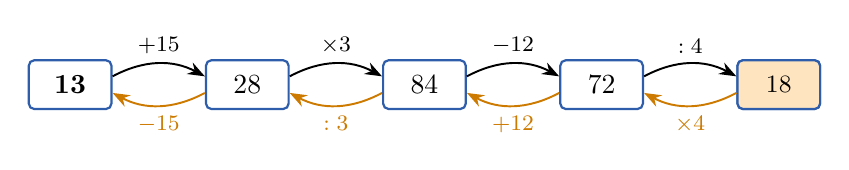
\begin{tikzpicture}[x=2.25cm,box/.style={draw=tmBlue!70!black,line width=0.8pt,rounded corners=2pt,minimum width=1.05cm,minimum height=0.62cm,font=\small}]
\foreach \v [count=\i from 0] in {?,28+15,84,72,18}{\node[box] (n\i) at (\i,0) {};}
\node at (n0) {$\mathbf{13}$}; \node at (n1) {$28$}; \node at (n2) {$84$}; \node at (n3) {$72$}; \node[box,fill=tmOrange!25] at (n4) {$18$};
\foreach \a/\b/\f/\g in {0/1/+15/-15,1/2/\times3/:3,2/3/-12/+12,3/4/:4/\times4}{
  \draw[-{Stealth},line width=0.7pt] ([yshift=3pt]n\a.east) to[bend left=28] node[above,font=\footnotesize]{$\f$} ([yshift=3pt]n\b.west);
  \draw[-{Stealth},line width=0.7pt,tmOrange!80!black] ([yshift=-3pt]n\b.west) to[bend left=28] node[below,font=\footnotesize]{$\g$} ([yshift=-3pt]n\a.east);}
\end{tikzpicture}
\end{center}
Tính ngược: $18\times4=72$;\par $72+12=84$;\par $84:3=28$;\par $28-15=13$.\par
\emph{Thử lại:} $(13+15)\times3=84$;\par $84-12=72$;\par $72:4=18$.
\dapso{$13$.}
\end{exbox}
\gap
\begin{exbox}{\ExWord\ 2}
Một bà mang trứng ra chợ bán. Lần đầu bà bán một nửa số trứng và thêm $1$ quả. Lần sau bà bán một nửa số trứng còn lại và thêm $1$ quả. Bà còn lại $10$ quả. Hỏi bà mang ra chợ bao nhiêu quả trứng?
\guide
\emph{Tính ngược lần bán thứ hai:} nếu không bán thêm quả trứng đó thì còn $10+1=11$ quả, đó là một nửa số trứng trước lần bán này.\par Vậy trước lần bán thứ hai: $11\times2=22$ quả.\par
\emph{Tính ngược lần bán thứ nhất:} $(22+1)\times2=46$ quả.
\dapso{$46$ quả trứng.}
\end{exbox}
\gap
\begin{exbox}{\ExWord\ 3}
Ngày thứ nhất dùng $\dfrac13$ lượng nước trong bể; ngày thứ hai dùng $\dfrac25$ lượng nước còn lại. Bây giờ bể còn $120$ lít. Hỏi lúc đầu bể có bao nhiêu lít nước?
\guide
Sau ngày thứ hai, còn lại $1-\dfrac25=\dfrac35$ lượng nước còn sau ngày thứ nhất.\par Lượng nước còn sau ngày thứ nhất là $120:\dfrac35=200$ lít.\par
$200$ lít là $1-\dfrac13=\dfrac23$ lượng nước ban đầu.\par Lúc đầu: $200:\dfrac23=300$ lít.
\dapso{$300$ lít.}
\end{exbox}
\gap
\begin{exbox}{\ExWord\ 4}
Ba thùng chứa $240$ lít dầu. Đầu tiên, thùng I rót sang thùng II một lượng dầu bằng lượng dầu thùng II đang có. Sau đó thùng II rót sang thùng III một lượng bằng lượng dầu thùng III đang có. Rồi thùng III rót sang thùng I một lượng bằng lượng dầu thùng I đang có. Lúc này ba thùng có lượng dầu bằng nhau. Hỏi lúc đầu mỗi thùng có bao nhiêu lít dầu?
\guide
Lúc cuối mỗi thùng có $240:3=80$ lít.\par Thùng nào ``nhận thêm bằng lượng đang có'' thì gấp đôi; khi tính ngược, ta \emph{chia đôi} thùng nhận và \emph{trả lại} lượng đó cho thùng rót.
\begin{center}
\renewcommand{\arraystretch}{1.25}
\begin{tabular}{|l|c|c|c|}
\hline
 & Thùng I & Thùng II & Thùng III\\\hline
Lúc cuối & $80$ & $80$ & $80$\\\hline
Trước bước 3 & $40$ & $80$ & $120$\\\hline
Trước bước 2 & $40$ & $140$ & $60$\\\hline
Lúc đầu & $\mathbf{110}$ & $\mathbf{70}$ & $\mathbf{60}$\\\hline
\end{tabular}
\end{center}
\dapso{Thùng I: $110$ lít; thùng II: $70$ lít; thùng III: $60$ lít.}
\end{exbox}
\dividerbar{Luyện tập}
\begin{probbox}{1}{\relax}
Tìm một số, biết rằng lấy số đó nhân với $4$, trừ đi $18$ rồi chia cho $2$ thì được $25$.
\end{probbox}
\probsol{
$25\times2=50$;\par $50+18=68$;\par $68:4=17$.
\dapso{$17$.}}
\gap
\begin{probbox}{2}{\relax}
Nam nghĩ ra một số. Bạn ấy nhân số đó với $6$, cộng thêm $8$, chia cho $2$ rồi trừ đi $14$ thì được $20$. Hỏi Nam đã nghĩ ra số nào?
\end{probbox}
\probsol{
$20+14=34$;\par $34\times2=68$;\par $68-8=60$;\par $60:6=10$.
\dapso{$10$.}}
\gap
\begin{probbox}{3}{\relax}
Tìm một số, biết rằng lấy số đó cộng với $\dfrac12$ rồi nhân với $\dfrac23$ thì được $3$.
\end{probbox}
\probsol{
$3:\dfrac23=\dfrac92$;\par $\dfrac92-\dfrac12=4$.
\dapso{$4$.}}
\gap
\begin{probbox}{4}{\relax}
Lấy tuổi của An gấp đôi, cộng thêm $5$ rồi chia cho $3$ thì được $9$. Hỏi An bao nhiêu tuổi?
\end{probbox}
\probsol{
$9\times3=27$;\par $27-5=22$;\par $22:2=11$.
\dapso{$11$ tuổi.}}
\gap
\begin{probbox}{5}{\relax}
Lan dùng $\dfrac12$ số tiền để mua sách và $\dfrac13$ số tiền còn lại để mua bút, còn lại $20\,000$ đồng. Hỏi lúc đầu Lan có bao nhiêu tiền?
\end{probbox}
\probsol{
$20\,000$ đồng là $\dfrac23$ số tiền còn lại sau khi mua sách, tức là\par $30\,000$ đồng.\par Lúc đầu: $30\,000\times2=60\,000$ đồng.
\dapso{$60\,000$ đồng.}}
\gap
\begin{probbox}{6}{\relax}
Ngày thứ nhất Hoa đọc $\dfrac14$ cuốn sách, ngày thứ hai đọc $\dfrac13$ số trang còn lại, ngày thứ ba đọc nốt $60$ trang cuối. Hỏi cuốn sách có bao nhiêu trang?
\end{probbox}
\probsol{
$60$ trang là $\dfrac23$ số trang còn lại sau ngày thứ nhất: $60:\dfrac23=90$.\par Và $90$ trang là $\dfrac34$ cuốn sách: $90:\dfrac34=120$.
\dapso{$120$ trang.}}
\gap
\begin{probbox}{7}{\relax}
Bác Ba bán một nửa số gà và thêm $2$ con, rồi bán một nửa số gà còn lại và thêm $2$ con, thì còn lại $8$ con. Hỏi lúc đầu bác Ba có bao nhiêu con gà?
\end{probbox}
\probsol{
Trước lần bán thứ hai: $(8+2)\times2=20$.\par Lúc đầu: $(20+2)\times2=44$.
\dapso{$44$ con gà.}}
\gap
\begin{probbox}{8}{\relax}
Đi chợ, lần đầu mẹ tiêu một nửa số tiền và thêm $5\,000$ đồng, lần sau tiêu một nửa số tiền còn lại và thêm $5\,000$ đồng, thì còn lại $10\,000$ đồng. Hỏi mẹ mang đi bao nhiêu tiền?
\end{probbox}
\probsol{
Trước lần mua thứ hai: $(10\,000+5\,000)\times2=30\,000$ đồng.\par Lúc đầu: $(30\,000+5\,000)\times2=70\,000$ đồng.
\dapso{$70\,000$ đồng.}}
\gap
\begin{probbox}{9}{\relax}
Rót $15$ lít từ bể A sang bể B, rồi rót $5$ lít từ bể B trở lại bể A. Lúc này mỗi bể có $40$ lít. Hỏi lúc đầu mỗi bể có bao nhiêu lít?
\end{probbox}
\probsol{
Bể A: $40-5+15=50$ lít; bể B: $40+5-15=30$ lít.
\dapso{A: $50$ lít; B: $30$ lít.}}
\gap
\begin{probbox}{10}{\relax}
Chuyển $6$ quả cam từ rổ I sang rổ II, rồi chuyển $2$ quả từ rổ II trở lại rổ I. Lúc này rổ I có $20$ quả và rổ II có $30$ quả. Hỏi lúc đầu mỗi rổ có bao nhiêu quả?
\end{probbox}
\probsol{
Rổ I: $20-2+6=24$; rổ II: $30+2-6=26$.
\dapso{$24$ quả và $26$ quả cam.}}
\gap
\begin{probbox}{11}{\relax}
Bình I rót một nửa số nước sang bình II; sau đó bình II rót $\dfrac13$ lượng nước đang có sang bình I. Lúc này bình I có $8$ lít và bình II có $12$ lít. Hỏi lúc đầu mỗi bình có bao nhiêu lít nước?
\end{probbox}
\probsol{
Trước lần rót thứ hai, bình II còn giữ $\dfrac23$, nên lúc đó có $12:\dfrac23=18$ lít và đã rót đi $6$ lít; bình I có $8-6=2$ lít.\par
Lúc đầu bình I có $2\times2=4$ lít và đã rót đi $2$ lít; bình II có $18-2=16$ lít.
\dapso{Bình I: $4$ lít; bình II: $16$ lít.}}
\gap
\begin{probbox}{12}{\relax}
Tìm một số: cộng với $7$, nhân với $5$, rồi trừ đi $10$ thì được $65$.
\end{probbox}
\probsol{
Trước khi trừ $10$: $65+10=75$.\par Trước khi nhân với $5$: $75:5=15$.\par Trước khi cộng $7$: $15-7=8$.
\dapso{$8$.}}
\gap
\begin{probbox}{13}{\relax}
Tìm một số: nhân với $3$, cộng thêm $12$, rồi chia cho $5$ thì được $9$.
\end{probbox}
\probsol{
Trước khi chia cho $5$: $9\times5=45$.\par Trước khi cộng $12$: $45-12=33$.\par Số cần tìm: $33:3=11$.
\dapso{$11$.}}
\gap
\begin{probbox}{14}{\relax}
Tìm một số: trừ đi $4$, nhân với $6$, rồi cộng thêm $3$ thì được $51$.
\end{probbox}
\probsol{
Trước khi cộng $3$: $51-3=48$.\par Trước khi nhân với $6$: $48:6=8$.\par Số cần tìm: $8+4=12$.
\dapso{$12$.}}
\gap
\begin{probbox}{15}{\relax}
Tìm một số: chia cho $2$, cộng thêm $15$, rồi nhân với $4$ thì được $100$.
\end{probbox}
\probsol{
Trước khi nhân với $4$: $100:4=25$.\par Trước khi cộng $15$: $25-15=10$.\par Số cần tìm: $10\times2=20$.
\dapso{$20$.}}
\gap
\begin{probbox}{16}{\relax}
Tìm $x$: nhân với $2{,}5$, rồi trừ đi $1{,}5$ thì được $8{,}5$.
\end{probbox}
\probsol{
Trước khi trừ $1{,}5$: $8{,}5+1{,}5=10$.\par $x=10:2{,}5=4$.
\dapso{$x=4$.}}
\gap
\begin{probbox}{17}{\relax}
Tìm một số thập phân: cộng thêm $2{,}4$, rồi nhân với $3$ thì được $12{,}6$.
\end{probbox}
\probsol{
Trước khi nhân với $3$: $12{,}6:3=4{,}2$.\par Số cần tìm: $4{,}2-2{,}4=1{,}8$.
\dapso{$1{,}8$.}}
\gap
\begin{probbox}{18}{\relax}
Mai mua một cuốn sách hết $25\,000$ đồng, được mẹ cho thêm $10\,000$ đồng, rồi mua một cái bút hết $8\,000$ đồng thì còn lại $17\,000$ đồng. Hỏi lúc đầu Mai có bao nhiêu tiền?
\end{probbox}
\probsol{
Trước khi mua bút: $17\,000+8\,000=25\,000$ đồng.\par Trước khi được mẹ cho: $25\,000-10\,000=15\,000$ đồng.\par Lúc đầu: $15\,000+25\,000=40\,000$ đồng.
\dapso{$40\,000$ đồng.}}
\gap
\begin{probbox}{19}{\relax}
Một xe buýt rời bến. Đến điểm dừng thứ nhất có $6$ người xuống và $4$ người lên; đến điểm dừng thứ hai có $10$ người xuống và $3$ người lên. Lúc này trên xe có $21$ hành khách. Hỏi lúc rời bến trên xe có bao nhiêu hành khách?
\end{probbox}
\probsol{
Trước điểm dừng thứ hai: $21-3+10=28$.\par Trước điểm dừng thứ nhất: $28-4+6=30$.
\dapso{$30$ hành khách.}}
\gap
\begin{probbox}{20}{\relax}
Lấy tuổi bố chia cho $4$ rồi cộng thêm $3$ thì được $13$. Hỏi bố bao nhiêu tuổi?
\end{probbox}
\probsol{
Trước khi cộng $3$: $13-3=10$.\par Tuổi bố: $10\times4=40$.
\dapso{$40$ tuổi.}}
\gap
\begin{probbox}{21}{\relax}
Lan tiêu $\dfrac13$ số tiền, rồi tiêu $\dfrac12$ số tiền còn lại, thì còn $25\,000$ đồng. Hỏi lúc đầu Lan có bao nhiêu tiền?
\end{probbox}
\probsol{
$25\,000$ đồng là $\dfrac12$ số tiền còn lại sau lần tiêu thứ nhất.\par Vậy sau lần tiêu thứ nhất còn $25\,000\times2=50\,000$ đồng.\par Số tiền đó là $\dfrac23$ số tiền ban đầu.\par Ban đầu: $50\,000:\dfrac23=75\,000$ đồng.
\dapso{$75\,000$ đồng.}}
\gap
\begin{probbox}{22}{\relax}
Ngày thứ nhất dùng $\dfrac14$ lượng nước trong bể; ngày thứ hai dùng $\dfrac13$ lượng nước còn lại. Bể còn $300$ lít. Hỏi lúc đầu bể có bao nhiêu lít nước?
\end{probbox}
\probsol{
$300$ lít là $\dfrac23$ lượng nước còn lại sau ngày thứ nhất.\par Sau ngày thứ nhất: $300:\dfrac23=450$ lít.\par Đó là $\dfrac34$ lượng nước ban đầu.\par Ban đầu: $450:\dfrac34=600$ lít.
\dapso{$600$ lít.}}
\gap
\begin{probbox}{23}{\relax}
Một người bán trứng, lần đầu bán một nửa số trứng và thêm $2$ quả, lần sau bán một nửa số còn lại và thêm $1$ quả, thì còn lại $9$ quả. Hỏi lúc đầu có bao nhiêu quả trứng?
\end{probbox}
\probsol{
Trước khi bán thêm $1$ quả: $9+1=10$, là một nửa số trứng còn lại sau lần bán thứ nhất.\par Sau lần bán thứ nhất: $10\times2=20$.\par Tương tự, $20+2=22$ là một nửa số trứng ban đầu.\par Ban đầu: $22\times2=44$.
\dapso{$44$ quả trứng.}}
\gap
\begin{probbox}{24}{\relax}
Chuyển $8$ quả bưởi từ rổ A sang rổ B, rồi chuyển $3$ quả từ rổ B sang rổ A. Lúc này rổ A có $25$ quả và rổ B có $35$ quả. Hỏi lúc đầu mỗi rổ có bao nhiêu quả?
\end{probbox}
\probsol{
Trước lần chuyển thứ hai: A $25-3=22$, B $35+3=38$.\par Lúc đầu: A $22+8=30$, B $38-8=30$.
\dapso{Mỗi rổ $30$ quả.}}
\gap
\begin{probbox}{25}{\relax}
Một cửa hàng ngày thứ nhất bán $\dfrac25$ số gạo, ngày thứ hai bán một nửa số gạo còn lại, thì còn $45$ kg. Hỏi lúc đầu cửa hàng có bao nhiêu ki-lô-gam gạo?
\end{probbox}
\probsol{
Sau ngày thứ nhất: $45\times2=90$ kg.\par Đó là $\dfrac35$ số gạo ban đầu.\par Ban đầu: $90:\dfrac35=150$ kg.
\dapso{$150$ kg.}}
\gap
\begin{probbox}{26}{\relax}
Tìm $x$, biết $\left(x-\dfrac13\right)\times\dfrac34=\dfrac12$.
\end{probbox}
\probsol{
$x-\dfrac13=\dfrac12:\dfrac34=\dfrac23$.\par $x=\dfrac23+\dfrac13=1$.
\dapso{$x=1$.}}
\gap
\begin{probbox}{27}{\relax}
An cho Bình $\dfrac13$ số bi của mình, rồi cho Chi $4$ viên thì còn lại $12$ viên. Hỏi lúc đầu An có bao nhiêu viên bi?
\end{probbox}
\probsol{
Trước khi cho Chi: $12+4=16$.\par Đó là $\dfrac23$ số bi ban đầu.\par Ban đầu: $16:\dfrac23=24$.
\dapso{$24$ viên bi.}}
\gap
\begin{probbox}{28}{\relax}
Tìm một số: nhân với $4$, cộng thêm $0{,}6$, rồi chia cho $2$ thì được $5{,}3$.
\end{probbox}
\probsol{
Trước khi chia cho $2$: $5{,}3\times2=10{,}6$.\par Trước khi cộng $0{,}6$: $10$.\par Số cần tìm: $10:4=2{,}5$.
\dapso{$2{,}5$.}}
\gap
\begin{probbox}{29}{\relax}
Từ một cuộn vải, lần đầu cắt đi $\dfrac14$, lần thứ hai cắt $5$ m, lần thứ ba cắt một nửa phần còn lại, thì còn $8$ m. Hỏi cuộn vải dài bao nhiêu mét?
\end{probbox}
\probsol{
Trước lần cắt thứ ba: $8\times2=16$ m.\par Trước lần cắt thứ hai: $16+5=21$ m.\par Đó là $\dfrac34$ cuộn vải.\par Cuộn vải: $21:\dfrac34=28$ m.
\dapso{$28$ m.}}
\gap
\begin{probbox}{30}{\relax}
Chú Tư bán $\dfrac13$ số vịt, rồi mua thêm $15$ con thì có $75$ con. Hỏi lúc đầu chú Tư có bao nhiêu con vịt?
\end{probbox}
\probsol{
Trước khi mua: $75-15=60$.\par Đó là $\dfrac23$ đàn vịt.\par Ban đầu: $60:\dfrac23=90$.
\dapso{$90$ con vịt.}}
\dividerbar{Thử thách -- Nâng cao}
\begin{probbox}{31}{\stars{1}}
Một cửa hàng bán $\dfrac13$ cuộn vải và thêm $2$ m, rồi bán một nửa phần còn lại và thêm $3$ m, thì còn $12$ m. Hỏi cuộn vải dài bao nhiêu mét?
\end{probbox}
\probsol{
Trước lần bán thứ hai: $(12+3)\times2=30$ m.\par Khi đó $30+2=32$ m là $\dfrac23$ cuộn vải, nên cuộn vải dài $32:\dfrac23=48$ m.
\dapso{$48$ m.}}
\gap
\begin{probbox}{32}{\stars{1}}
Một chú khỉ hái được một số quả đào. Mỗi ngày khỉ ăn một nửa số đào đang có và thêm $1$ quả. Sáng ngày thứ năm khỉ chỉ còn đúng $1$ quả. Hỏi khỉ đã hái được bao nhiêu quả đào?
\end{probbox}
\probsol{
Khỉ đã ăn trong $4$ ngày.\par Tính ngược mỗi ngày bằng (số còn lại $+1$)$\times2$.\par
$1\to4\to10\to22\to46$.
\dapso{$46$ quả đào.}}
\gap
\begin{probbox}{33}{\stars{1}}
An, Bình và Cường có $96$ viên bi. An cho Bình số bi bằng số bi Bình đang có; rồi Bình cho Cường số bi bằng số bi Cường đang có; cuối cùng Cường cho An số bi bằng số bi An đang có. Lúc này số bi của ba bạn bằng nhau. Hỏi lúc đầu mỗi bạn có bao nhiêu viên bi?
\end{probbox}
\probsol{
Lúc cuối mỗi bạn có $32$ viên.\par Tính ngược từ cuối (như Ví dụ $4$):\par
Trước bước 3: An $16$, Bình $32$, Cường $48$.\par Trước bước 2: An $16$, Bình $56$, Cường $24$.\par Lúc đầu: An $44$, Bình $28$, Cường $24$.
\dapso{An: $44$; Bình: $28$; Cường: $24$ viên bi.}}
\gap
\begin{probbox}{34}{\stars{2}}
A, B và C chơi ba ván. Sau mỗi ván, người thua phải cho mỗi người còn lại số bi bằng số bi người đó đang có. A thua ván 1, B thua ván 2 và C thua ván 3. Sau đó mỗi người có $24$ viên bi. Hỏi lúc đầu mỗi người có bao nhiêu viên bi?
\end{probbox}
\probsol{
Tổng cộng: $72$ viên bi.\par Tính ngược, ở mỗi ván hai người thắng chia đôi số bi và người thua nhận lại số bi đó.\par
Trước ván 3: A $12$, B $12$, C $48$.\par Trước ván 2: A $6$, B $42$, C $24$.\par Lúc đầu: A $39$, B $21$, C $12$.
\dapso{A: $39$; B: $21$; C: $12$ viên bi.}}
\gap
\begin{probbox}{35}{\stars{1}}
Mỗi ngày một chú khỉ ăn một nửa số đào đang có và thêm $2$ quả. Sau $3$ ngày khỉ còn $3$ quả. Hỏi lúc đầu khỉ có bao nhiêu quả đào?
\end{probbox}
\probsol{
Đầu ngày thứ ba: $(3+2)\times2=10$.\par Đầu ngày thứ hai: $(10+2)\times2=24$.\par Lúc đầu: $(24+2)\times2=52$.
\dapso{$52$ quả đào.}}
\gap
\begin{probbox}{36}{\stars{1}}
Rót từ bình A sang bình B một lượng bằng lượng nước bình B đang có; rồi rót từ bình B sang bình A một lượng bằng lượng nước bình A đang có. Lúc này mỗi bình có $24$ lít. Hỏi lúc đầu mỗi bình có bao nhiêu lít?
\end{probbox}
\probsol{
Lần rót thứ hai làm bình A gấp đôi, nên trước đó A có $24:2=12$ và B có $24+12=36$.\par Lần rót thứ nhất làm bình B gấp đôi, nên trước đó B có $36:2=18$ và A có $12+18=30$.
\dapso{A $30$ lít, B $18$ lít.}}
\gap
\begin{probbox}{37}{\stars{1}}
Một cửa hàng bán một nửa số gạo và thêm $5$ kg, rồi bán $\dfrac13$ số gạo còn lại và thêm $4$ kg, rồi bán $\dfrac14$ số gạo còn lại và thêm $3$ kg, thì còn $15$ kg. Hỏi lúc đầu có bao nhiêu ki-lô-gam gạo?
\end{probbox}
\probsol{
Trước lần bán thứ ba: $15+3=18$ kg là $\dfrac34$, nên có $18:\dfrac34=24$ kg.\par Trước lần bán thứ hai: $24+4=28$ kg là $\dfrac23$, nên có $42$ kg.\par Lúc đầu: $(42+5)\times2=94$ kg.
\dapso{$94$ kg.}}
\gap
\begin{probbox}{38}{\stars{1}}
Nam nghĩ ra một số. Ba lần liên tiếp, bạn ấy gấp đôi số đó rồi trừ đi $3$, cuối cùng được $19$. Hỏi Nam đã nghĩ ra số nào?
\end{probbox}
\probsol{
Trước lượt thứ ba: $(19+3):2=11$.\par Trước lượt thứ hai: $(11+3):2=7$.\par Số cần tìm: $(7+3):2=5$.
\dapso{$5$.}}
\gap
\begin{probbox}{39}{\stars{1}}
Một đội sửa đường: tuần thứ nhất sửa $\dfrac14$ quãng đường và thêm $3$ km; tuần thứ hai sửa $\dfrac13$ phần còn lại và thêm $1$ km; tuần thứ ba sửa nốt $9$ km cuối. Hỏi quãng đường dài bao nhiêu ki-lô-mét?
\end{probbox}
\probsol{
Sau tuần thứ nhất, $9+1=10$ km là $\dfrac23$ phần còn lại, nên phần còn lại là $15$ km.\par $15+3=18$ km là $\dfrac34$ quãng đường.\par Quãng đường: $18:\dfrac34=24$ km.
\dapso{$24$ km.}}
\gap
\begin{probbox}{40}{\stars{1}}
Cô Hạnh dùng $\dfrac25$ tiền lương cho ăn uống, $\dfrac13$ số còn lại cho việc học của con và gửi tiết kiệm một nửa số còn lại, thì còn giữ $1\,200\,000$ đồng. Hỏi tiền lương của cô là bao nhiêu?
\end{probbox}
\probsol{
Trước khi gửi tiết kiệm: $1\,200\,000\times2=2\,400\,000$ đồng.\par Trước khi chi cho việc học: $2\,400\,000:\dfrac23=3\,600\,000$ đồng.\par Tiền lương: $3\,600\,000:\dfrac35=6\,000\,000$ đồng.
\dapso{$6\,000\,000$ đồng.}}
\gap
\begin{probbox}{41}{\stars{1}}
Lấy tuổi của ông trừ đi $4$, chia cho $7$, cộng thêm $2$, rồi nhân với $5$ thì được $60$. Hỏi ông bao nhiêu tuổi?
\end{probbox}
\probsol{
Trước khi $\times5$: $12$.\par Trước khi $+2$: $10$.\par Trước khi $:7$: $70$.\par Tuổi ông: $70+4=74$.
\dapso{$74$ tuổi.}}
\gap
\begin{probbox}{42}{\stars{1}}
Bèo tấm mỗi ngày tăng diện tích gấp đôi và phủ kín cả ao vào cuối ngày thứ $10$. Hỏi vào ngày thứ mấy bèo phủ được $\dfrac14$ mặt ao?
\end{probbox}
\probsol{
Cuối ngày thứ $9$ bèo phủ $\dfrac12$ mặt ao (gấp đôi lên thì phủ kín).\par Cuối ngày thứ $8$ bèo phủ $\dfrac14$ mặt ao.
\dapso{Ngày thứ $8$.}}
\gap
\begin{probbox}{43}{\stars{1}}
Ba thùng chứa $180$ lít. Rót $10$ l từ thùng I sang thùng II, rồi $20$ l từ thùng II sang thùng III, rồi $5$ l từ thùng III sang thùng I. Lúc này ba thùng bằng nhau. Hỏi lúc đầu mỗi thùng chứa bao nhiêu lít?
\end{probbox}
\probsol{
Lúc cuối mỗi thùng có $180:3=60$ l.\par Trước lần rót thứ ba: I $55$, III $65$.\par Trước lần rót thứ hai: II $80$, III $45$.\par Lúc đầu: I $65$, II $70$, III $45$.
\dapso{I $65$ l, II $70$ l, III $45$ l.}}
\gap
\begin{probbox}{44}{\stars{1}}
Tìm $x$, biết $(x\times1{,}5-2{,}25):0{,}5=7{,}5$.
\end{probbox}
\probsol{
$x\times1{,}5-2{,}25=7{,}5\times0{,}5=3{,}75$.\par $x\times1{,}5=6$.\par $x=4$.
\dapso{$x=4$.}}
\gap
\begin{probbox}{45}{\stars{1}}
Bà tiêu một nửa số tiền và thêm $3\,000$ đồng, rồi một nửa số còn lại và thêm $2\,000$ đồng, rồi một nửa số còn lại và thêm $1\,000$ đồng thì hết tiền. Hỏi bà mang đi bao nhiêu tiền?
\end{probbox}
\probsol{
Trước lần tiêu thứ ba: $(0+1\,000)\times2=2\,000$ đồng.\par Trước lần tiêu thứ hai: $(2\,000+2\,000)\times2=8\,000$ đồng.\par Lúc đầu: $(8\,000+3\,000)\times2=22\,000$ đồng.
\dapso{$22\,000$ đồng.}}
\gap
\begin{probbox}{46}{\stars{1}}
Hai rổ có $60$ quả cam. Chuyển $\dfrac13$ số cam rổ I sang rổ II, rồi chuyển $\dfrac14$ số cam rổ II (lúc đó) sang rổ I. Lúc này số cam hai rổ bằng nhau. Hỏi lúc đầu mỗi rổ có bao nhiêu quả?
\end{probbox}
\probsol{
Lúc cuối mỗi rổ có $30$ quả.\par Trước lần chuyển thứ hai, rổ II có $30:\dfrac34=40$, nên rổ I có $20$.\par Trước lần chuyển thứ nhất, rổ I có $20:\dfrac23=30$, nên rổ II có $30$.
\dapso{Mỗi rổ $30$ quả.}}
\gap
\begin{probbox}{47}{\stars{1}}
Hà làm toán trong $45$ phút, nghỉ $15$ phút, rồi đọc sách trong $1$ giờ $20$ phút, xong lúc $21{:}05$. Hỏi Hà bắt đầu lúc mấy giờ?
\end{probbox}
\probsol{
Bắt đầu đọc sách lúc $21{:}05-1{:}20=19{:}45$.\par Bắt đầu nghỉ lúc $19{:}30$.\par Bắt đầu làm toán lúc $18{:}45$.
\dapso{$18{:}45$.}}
\gap
\begin{probbox}{48}{\stars{1}}
Nghĩ ra một số bất kì, nhân với $9$, cộng thêm $18$, chia cho $9$, rồi trừ đi số đã nghĩ. Chứng tỏ rằng kết quả luôn bằng $2$.
\end{probbox}
\probsol{
Gọi số đã nghĩ là $a$.\par $a\times9+18=(a+2)\times9$.\par Chia cho $9$: $a+2$.\par Trừ đi $a$: $2$, dù $a$ là số nào.
\dapso{Luôn bằng $2$.}}
\gap
\begin{probbox}{49}{\stars{2}}
Một con ốc sên ở đáy một cái giếng sâu $10$ m, ban ngày leo lên được $3$ m, ban đêm tụt xuống $2$ m. Hỏi đến ngày thứ mấy ốc sên lên tới miệng giếng?
\end{probbox}
\probsol{
Tính ngược từ ngày cuối: ốc sên leo $3$ m thì lên tới miệng giếng, nên đầu ngày đó nó ở độ cao $10-3=7$ m.\par Mỗi ngày đêm ốc sên lên được $3-2=1$ m.\par Để lên tới $7$ m cần $7$ ngày đêm.\par Vậy ốc sên ra khỏi giếng vào ngày thứ $8$.
\dapso{Ngày thứ $8$.}}
\gap
\begin{probbox}{50}{\stars{2}}
Bà có một số quả táo. Người con cả lấy một nửa số táo và thêm nửa quả; người con thứ hai lấy một nửa số còn lại và thêm nửa quả; người con út lấy một nửa số còn lại và thêm nửa quả thì vừa hết. Không quả táo nào bị cắt. Hỏi lúc đầu bà có bao nhiêu quả táo?
\end{probbox}
\probsol{
Trước khi người con út lấy: $\left(0+\dfrac12\right)\times2=1$.\par Trước khi người con thứ hai lấy: $\left(1+\dfrac12\right)\times2=3$.\par Lúc đầu: $\left(3+\dfrac12\right)\times2=7$.\par Thử lại: các con lấy $4$, $2$ và $1$ quả táo nguyên.
\dapso{$7$ quả táo.}}
\clearpage
\titlehead
\begingroup\setbox0=\vbox{\section*{Hình tam giác. Diện tích hình tam giác}}\endgroup
\chapterhead{11}{Hình tam giác. Diện tích hình tam giác}

\shead{Đáy, chiều cao và diện tích}
\begin{knowbox}
\begin{minipage}[t]{0.6\linewidth}
\textbf{Hình tam giác} có $3$ cạnh, $3$ đỉnh và $3$ góc. Theo góc, có hình tam giác \emph{nhọn} (ba góc nhọn), hình tam giác \emph{tù} (một góc tù) và hình tam giác \emph{vuông} (một góc vuông).\par
\smallskip
Đoạn thẳng kẻ từ một đỉnh và \textbf{vuông góc} với cạnh đối diện là \textbf{đường cao}; cạnh đó là \textbf{cạnh đáy}. Mỗi hình tam giác có $3$ đường cao.\par
\smallskip
\textbf{Diện tích hình tam giác} bằng độ dài đáy nhân với chiều cao (cùng một đơn vị đo) rồi chia cho $2$:
\[S=\frac{a\times h}{2}\qquad h=\frac{S\times2}{a}\qquad a=\frac{S\times2}{h}\]
Trong hình tam giác vuông, hai cạnh góc vuông là đáy và chiều cao của nhau.
\end{minipage}\hfill
\begin{minipage}[t]{0.36\linewidth}\vspace{2pt}
\centering
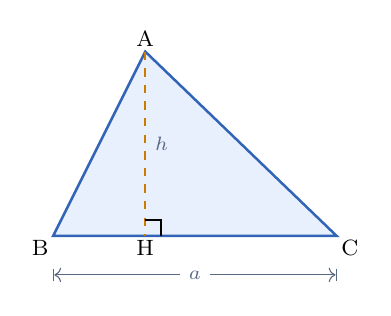
\begin{tikzpicture}[scale=0.9]
\coordinate (B) at (0,0); \coordinate (C) at (4,0); \coordinate (A) at (1.3,2.6); \coordinate (H) at (1.3,0);
\fill[tmBlue!12] (A)--(B)--(C)--cycle;
\draw[geo] (A)--(B)--(C)--cycle;
\draw[dashed,line width=0.7pt,tmOrange!80!black] (A)--(H);
\ramark{H}{C}{A}
\node[lbl,above] at (A){A}; \node[lbl,below left] at (B){B}; \node[lbl,below right] at (C){C}; \node[lbl,below] at (H){H};
\node[dim,right] at (1.3,1.3){$h$};
\draw[|<->|,Slate] (0,-0.55)--node[fill=white,dim]{$a$}(4,-0.55);
\end{tikzpicture}
\end{minipage}
\end{knowbox}
\gap
\begin{exbox}{\ExWord\ 1}
Tính diện tích hình tam giác có:
\begin{cols2}
\pa{a} độ dài đáy $8$ cm, chiều cao $5$ cm; & \pa{b} độ dài đáy $2{,}5$ dm, chiều cao $12$ cm.
\end{cols2}
\guide
\pa{a} $S=8\times5:2=20$ cm$^2$.\par
\pa{b} Trước hết đổi về cùng đơn vị đo: $2{,}5$ dm $=25$ cm.\par $S=25\times12:2=150$ cm$^2$.
\dapso{\pa{a} $20$ cm$^2$;\par \pa{b} $150$ cm$^2$.}
\end{exbox}
\gap
\begin{exbox}{\ExWord\ 2}
\begin{minipage}[t]{0.62\linewidth}
Hình tam giác ABC vuông tại A có $AB=6$ cm, $AC=8$ cm và $BC=10$ cm. Tính diện tích hình tam giác đó và độ dài đường cao AH.
\end{minipage}\hfill
\begin{minipage}[t]{0.34\linewidth}\vspace{0pt}\centering
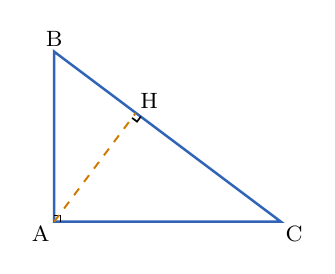
\begin{tikzpicture}[scale=0.36]
\coordinate (A) at (0,0); \coordinate (B) at (0,6); \coordinate (C) at (8,0); \coordinate (H) at (2.88,3.84);
\draw[geo] (A)--(B)--(C)--cycle; \ramark{A}{B}{C}
\draw[dashed,line width=0.7pt,tmOrange!80!black] (A)--(H); \ramark{H}{C}{A}
\node[lbl,below left] at (A){A}; \node[lbl,above] at (B){B}; \node[lbl,below right] at (C){C}; \node[lbl,above right] at (H){H};
\end{tikzpicture}
\end{minipage}
\guide
Lấy AC làm đáy thì AB là chiều cao: $S=6\times8:2=24$ cm$^2$.\par
Lấy BC làm đáy thì AH là chiều cao: $AH=24\times2:10=4{,}8$ cm.
\dapso{$24$ cm$^2$;\par $AH=4{,}8$ cm.}
\end{exbox}
\gap
\begin{exbox}{\ExWord\ 3}
Một hình tam giác có diện tích $36$ cm$^2$ và độ dài đáy $9$ cm. Tính chiều cao của hình tam giác đó.
\guide
$h=S\times2:a=36\times2:9=8$ cm.
\dapso{$8$ cm.}
\end{exbox}
\gap
\begin{exbox}{\ExWord\ 4}
\begin{minipage}[t]{0.6\linewidth}
Hình chữ nhật ABCD có $AB=12$ cm và $BC=8$ cm; M là trung điểm của BC. Tính diện tích các hình tam giác ABM, MCD và AMD.
\end{minipage}\hfill
\begin{minipage}[t]{0.36\linewidth}\vspace{0pt}\centering
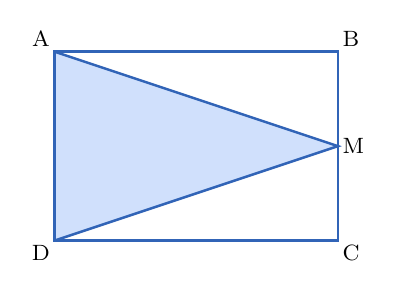
\begin{tikzpicture}[scale=0.3]
\coordinate (A) at (0,8); \coordinate (B) at (12,8); \coordinate (C) at (12,0); \coordinate (D) at (0,0); \coordinate (M) at (12,4);
\fill[shade] (A)--(M)--(D)--cycle;
\draw[geo] (A)--(B)--(C)--(D)--cycle; \draw[geo] (A)--(M)--(D);
\node[lbl,above left] at (A){A}; \node[lbl,above right] at (B){B}; \node[lbl,below right] at (C){C}; \node[lbl,below left] at (D){D}; \node[lbl,right] at (M){M};
\end{tikzpicture}
\end{minipage}
\guide
$BM=MC=8:2=4$ cm.\par $S_{ABM}=12\times4:2=24$ cm$^2$;\par $S_{MCD}=12\times4:2=24$ cm$^2$.\par
$S_{ABCD}=12\times8=96$ cm$^2$, nên $S_{AMD}=96-24-24=48$ cm$^2$.\par
\emph{Nhận xét:} hình tam giác AMD có đáy AD và chiều cao bằng AB, nên diện tích của nó bằng một nửa diện tích hình chữ nhật.
\dapso{$24$ cm$^2$; $24$ cm$^2$; $48$ cm$^2$.}
\end{exbox}
\dividerbar{Luyện tập}
\begin{probbox}{1}{\relax}
Tính diện tích hình tam giác có độ dài đáy $a$ và chiều cao $h$:
\begin{cols2}
\pa{a} $a=15$ cm, $h=8$ cm; & \pa{b} $a=4{,}5$ m, $h=2$ m;\\
\pa{c} $a=\dfrac34$ m, $h=\dfrac25$ m; & \pa{d} $a=1{,}2$ dm, $h=15$ cm.
\end{cols2}
\end{probbox}
\probsol{
\pa{a} $15\times8:2=60$ cm$^2$.\par \pa{b} $4{,}5\times2:2=4{,}5$ m$^2$.\par \pa{c} $\dfrac34\times\dfrac25:2=\dfrac3{20}$ m$^2$.\par \pa{d} $1{,}2$ dm $=12$ cm; $12\times15:2=90$ cm$^2$.
\dapso{$60$ cm$^2$; $4{,}5$ m$^2$; $\dfrac3{20}$ m$^2$; $90$ cm$^2$.}}
\gap
\begin{probbox}{2}{\relax}
Tính diện tích hình tam giác vuông có hai cạnh góc vuông dài $3{,}5$ dm và $2$ dm.
\end{probbox}
\probsol{
$S=3{,}5\times2:2=3{,}5$ dm$^2$.
\dapso{$3{,}5$ dm$^2$.}}
\gap
\begin{probbox}{3}{\relax}
Một hình tam giác có diện tích $45$ cm$^2$ và chiều cao $6$ cm. Tính độ dài đáy của hình tam giác đó.
\end{probbox}
\probsol{
$a=45\times2:6=15$ cm.
\dapso{$15$ cm.}}
\gap
\begin{probbox}{4}{\relax}
Một mảnh đất hình tam giác có độ dài đáy $40$ m, chiều cao bằng $\dfrac34$ độ dài đáy. Tính diện tích mảnh đất đó.
\end{probbox}
\probsol{
Chiều cao: $40\times\dfrac34=30$ m.\par Diện tích: $40\times30:2=600$ m$^2$.
\dapso{$600$ m$^2$.}}
\gap
\begin{probbox}{5}{\relax}
Một tấm bìa hình tam giác có độ dài đáy $2{,}4$ dm, chiều cao bằng $\dfrac23$ độ dài đáy. Tính diện tích tấm bìa đó.
\end{probbox}
\probsol{
Chiều cao: $2{,}4\times\dfrac23=1{,}6$ dm.\par Diện tích: $2{,}4\times1{,}6:2=1{,}92$ dm$^2$.
\dapso{$1{,}92$ dm$^2$.}}
\gap
\begin{probbox}{6}{\relax}
Hình tam giác ABC vuông tại A có $AB=9$ cm, $AC=12$ cm và $BC=15$ cm. Tính độ dài đường cao AH.
\end{probbox}
\probsol{
$S=9\times12:2=54$ cm$^2$.\par $AH=54\times2:15=7{,}2$ cm.
\dapso{$7{,}2$ cm.}}
\gap
\begin{probbox}{7}{\relax}
Một hình tam giác có diện tích bằng diện tích hình vuông cạnh $6$ cm. Độ dài đáy của hình tam giác là $9$ cm. Tính chiều cao của hình tam giác đó.
\end{probbox}
\probsol{
Diện tích: $6\times6=36$ cm$^2$.\par Chiều cao: $36\times2:9=8$ cm.
\dapso{$8$ cm.}}
\gap
\begin{probbox}{8}{\relax}
Một hình tam giác có độ dài đáy $18$ cm. Nếu kéo dài đáy thêm $4$ cm (giữ nguyên chiều cao) thì diện tích tăng thêm $20$ cm$^2$. Tính diện tích hình tam giác ban đầu.
\end{probbox}
\probsol{
Phần tăng thêm là hình tam giác có đáy $4$ cm và diện tích $20$ cm$^2$; chiều cao của nó là $20\times2:4=10$ cm.\par
Diện tích ban đầu: $18\times10:2=90$ cm$^2$.
\dapso{$90$ cm$^2$.}}
\gap
\begin{probbox}{9}{\relax}
Hình vuông ABCD có cạnh $10$ cm; M là trung điểm của BC. Tính diện tích hình tam giác ABM và hình tứ giác AMCD.
\end{probbox}
\probsol{
$S_{ABM}=10\times5:2=25$ cm$^2$.\par $S_{AMCD}=10\times10-25=75$ cm$^2$.
\dapso{$25$ cm$^2$; $75$ cm$^2$.}}
\gap
\begin{probbox}{10}{\relax}
Hình tam giác ABC có diện tích $60$ cm$^2$ và $BC=15$ cm. Điểm M nằm trên BC sao cho $BM=5$ cm. Tính diện tích hình tam giác ABM.
\end{probbox}
\probsol{
Chiều cao hạ từ A xuống BC là $60\times2:15=8$ cm.\par Hình tam giác ABM có cùng chiều cao đó: $S_{ABM}=5\times8:2=20$ cm$^2$.
\dapso{$20$ cm$^2$.}}
\gap
\begin{probbox}{11}{\relax}
\begin{minipage}[t]{0.62\linewidth}
Trong hình bên có bao nhiêu hình tam giác? Hãy kể tên các hình tam giác đó.
\end{minipage}\hfill
\begin{minipage}[t]{0.34\linewidth}\vspace{0pt}\centering
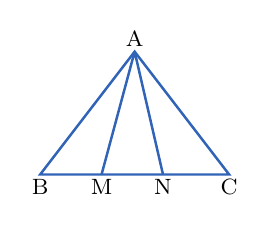
\begin{tikzpicture}[scale=0.6]
\coordinate (A) at (2,2.6); \coordinate (B) at (0,0); \coordinate (M) at (1.3,0); \coordinate (N) at (2.6,0); \coordinate (C) at (4,0);
\draw[geo] (A)--(B)--(C)--cycle; \draw[geo] (A)--(M) (A)--(N);
\node[lbl,above] at (A){A}; \node[lbl,below] at (B){B}; \node[lbl,below] at (M){M}; \node[lbl,below] at (N){N}; \node[lbl,below] at (C){C};
\end{tikzpicture}
\end{minipage}
\end{probbox}
\probsol{
Mỗi hình tam giác có đỉnh A và đáy là đoạn thẳng nối hai trong bốn điểm B, M, N, C.\par Có $3+2+1=6$ đoạn thẳng như vậy.\par
Các hình tam giác: ABM, AMN, ANC, ABN, AMC, ABC.
\dapso{$6$ hình tam giác.}}
\gap
\begin{probbox}{12}{\relax}
Tính diện tích hình tam giác có độ dài đáy $14$ cm và chiều cao $9$ cm.
\end{probbox}
\probsol{
$S=14\times9:2=63$ cm$^2$.
\dapso{$63$ cm$^2$.}}
\gap
\begin{probbox}{13}{\relax}
Tính diện tích hình tam giác có độ dài đáy $2{,}5$ m và chiều cao $1{,}6$ m.
\end{probbox}
\probsol{
$S=2{,}5\times1{,}6:2=2$ m$^2$.
\dapso{$2$ m$^2$.}}
\gap
\begin{probbox}{14}{\relax}
Tính diện tích hình tam giác có độ dài đáy $\dfrac34$ m và chiều cao $\dfrac25$ m.
\end{probbox}
\probsol{
$S=\dfrac34\times\dfrac25:2=\dfrac3{20}$ m$^2$.
\dapso{$\dfrac3{20}$ m$^2$.}}
\gap
\begin{probbox}{15}{\relax}
Tính diện tích hình tam giác có độ dài đáy $3$ dm và chiều cao $25$ cm.
\end{probbox}
\probsol{
$3$ dm $=30$ cm.\par $S=30\times25:2=375$ cm$^2$.
\dapso{$375$ cm$^2$.}}
\gap
\begin{probbox}{16}{\relax}
Tính diện tích hình tam giác vuông có hai cạnh góc vuông dài $7$ cm và $10$ cm.
\end{probbox}
\probsol{
Một cạnh góc vuông là đáy, cạnh góc vuông kia là chiều cao.\par $S=7\times10:2=35$ cm$^2$.
\dapso{$35$ cm$^2$.}}
\gap
\begin{probbox}{17}{\relax}
Một hình tam giác có diện tích $54$ cm$^2$ và độ dài đáy $12$ cm. Tính chiều cao của hình tam giác đó.
\end{probbox}
\probsol{
Chiều cao $=$ diện tích $\times2\,:$ độ dài đáy.\par $h=54\times2:12=9$ cm.
\dapso{$9$ cm.}}
\gap
\begin{probbox}{18}{\relax}
Một hình tam giác có diện tích $7{,}5$ dm$^2$ và chiều cao $2{,}5$ dm. Tính độ dài đáy của hình tam giác đó.
\end{probbox}
\probsol{
Độ dài đáy $=$ diện tích $\times2\,:$ chiều cao.\par $a=7{,}5\times2:2{,}5=6$ dm.
\dapso{$6$ dm.}}
\gap
\begin{probbox}{19}{\relax}
Một thửa ruộng hình tam giác có độ dài đáy $50$ m và chiều cao $24$ m. Cứ mỗi mét vuông thu hoạch được $0{,}8$ kg rau. Hỏi trên cả thửa ruộng đó thu hoạch được bao nhiêu ki-lô-gam rau?
\end{probbox}
\probsol{
Diện tích: $50\times24:2=600$ m$^2$.\par Số rau thu hoạch được: $0{,}8\times600=480$ kg.
\dapso{$480$ kg.}}
\gap
\begin{probbox}{20}{\relax}
Một hình tam giác có độ dài đáy $16$ cm, chiều cao bằng $\dfrac34$ độ dài đáy. Tính diện tích hình tam giác đó.
\end{probbox}
\probsol{
Chiều cao: $16\times\dfrac34=12$ cm.\par Diện tích: $16\times12:2=96$ cm$^2$.
\dapso{$96$ cm$^2$.}}
\gap
\begin{probbox}{21}{\relax}
Tổng độ dài đáy và chiều cao của một hình tam giác là $30$ cm, độ dài đáy hơn chiều cao $6$ cm. Tính diện tích hình tam giác đó.
\end{probbox}
\probsol{
Độ dài đáy: $(30+6):2=18$ cm.\par Chiều cao: $12$ cm.\par Diện tích: $18\times12:2=108$ cm$^2$.
\dapso{$108$ cm$^2$.}}
\gap
\begin{probbox}{22}{\relax}
Hình tam giác ABC vuông tại A có $AB=15$ cm, $AC=20$ cm, $BC=25$ cm. Tính diện tích hình tam giác đó và độ dài đường cao AH.
\end{probbox}
\probsol{
Diện tích: $15\times20:2=150$ cm$^2$.\par Lấy BC làm đáy thì AH là chiều cao.\par $AH=150\times2:25=12$ cm.
\dapso{$150$ cm$^2$; $AH=12$ cm.}}
\gap
\begin{probbox}{23}{\relax}
Hình tam giác thứ nhất có độ dài đáy $12$ cm và chiều cao $8$ cm. Hình tam giác thứ hai có cùng diện tích và có độ dài đáy $16$ cm. Tính chiều cao của hình tam giác thứ hai.
\end{probbox}
\probsol{
Diện tích: $12\times8:2=48$ cm$^2$.\par Chiều cao của hình tam giác thứ hai: $48\times2:16=6$ cm.
\dapso{$6$ cm.}}
\gap
\begin{probbox}{24}{\relax}
Mỗi lá cờ hình tam giác có độ dài đáy $30$ cm và chiều cao $20$ cm. Hỏi làm $20$ lá cờ như thế cần bao nhiêu đề-xi-mét vuông vải? (Không tính phần đường may.)
\end{probbox}
\probsol{
Một lá cờ: $30\times20:2=300$ cm$^2$.\par $20$ lá cờ: $6\,000$ cm$^2$ $=60$ dm$^2$.
\dapso{$60$ dm$^2$.}}
\gap
\begin{probbox}{25}{\relax}
Một hình tam giác vuông có diện tích $24$ cm$^2$ và một cạnh góc vuông dài $6$ cm. Tính độ dài cạnh góc vuông còn lại.
\end{probbox}
\probsol{
Cạnh góc vuông còn lại là chiều cao ứng với đáy $6$ cm.\par Độ dài: $24\times2:6=8$ cm.
\dapso{$8$ cm.}}
\gap
\begin{probbox}{26}{\relax}
Hình chữ nhật ABCD có chiều dài $12$ cm, chiều rộng $8$ cm. Đường chéo AC chia hình chữ nhật thành hai hình tam giác. Tính diện tích mỗi hình tam giác.
\end{probbox}
\probsol{
Hình tam giác ABC vuông tại B có hai cạnh góc vuông dài $12$ cm và $8$ cm.\par $S_{ABC}=12\times8:2=48$ cm$^2$.\par Tương tự, $S_{ACD}=48$ cm$^2$ (bằng một nửa diện tích hình chữ nhật).
\dapso{Mỗi hình $48$ cm$^2$.}}
\gap
\begin{probbox}{27}{\relax}
Một hình tam giác có diện tích $150$ cm$^2$. Nếu tăng chiều cao thêm $3$ cm (giữ nguyên đáy) thì diện tích tăng thêm $30$ cm$^2$. Tính độ dài đáy và chiều cao của hình tam giác đó.
\end{probbox}
\probsol{
Phần tăng thêm là hình tam giác có cùng đáy, chiều cao $3$ cm và diện tích $30$ cm$^2$.\par Độ dài đáy: $30\times2:3=20$ cm.\par Chiều cao: $150\times2:20=15$ cm.
\dapso{Đáy $20$ cm, chiều cao $15$ cm.}}
\gap
\begin{probbox}{28}{\relax}
Một hình tam giác có độ dài đáy $8$ cm và có diện tích bằng diện tích hình vuông cạnh $8$ cm. Tính chiều cao của hình tam giác đó.
\end{probbox}
\probsol{
Hình vuông: $8\times8=64$ cm$^2$.\par Chiều cao: $64\times2:8=16$ cm.
\dapso{$16$ cm.}}
\gap
\begin{probbox}{29}{\relax}
Một cánh đồng hình tam giác có độ dài đáy $120$ m và chiều cao $80$ m. Tính diện tích cánh đồng đó theo đơn vị héc-ta.
\end{probbox}
\probsol{
Diện tích: $120\times80:2=4\,800$ m$^2$.\par $1$ ha $=10\,000$ m$^2$, nên diện tích đó là $0{,}48$ ha.
\dapso{$0{,}48$ ha.}}
\gap
\begin{probbox}{30}{\relax}
Hình tam giác ABC có diện tích $48$ cm$^2$; M là trung điểm của BC. Tính diện tích hình tam giác ABM.
\end{probbox}
\probsol{
ABM và ABC chung chiều cao hạ từ A.\par $BM=\dfrac12BC$, nên $S_{ABM}=\dfrac12S_{ABC}$.\par $S_{ABM}=48:2=24$ cm$^2$.
\dapso{$24$ cm$^2$.}}
\dividerbar{Thử thách -- Nâng cao}
\begin{probbox}{31}{\stars{1}}
Một hình tam giác có diện tích $120$ cm$^2$. Nếu giảm độ dài đáy đi $3$ cm (giữ nguyên chiều cao) thì diện tích giảm đi $18$ cm$^2$. Tính độ dài đáy.
\end{probbox}
\probsol{
Chiều cao: $18\times2:3=12$ cm.\par Độ dài đáy: $120\times2:12=20$ cm.
\dapso{$20$ cm.}}
\gap
\begin{probbox}{32}{\stars{1}}
Tổng độ dài hai cạnh góc vuông của một hình tam giác vuông là $14$ cm, cạnh này dài hơn cạnh kia $2$ cm. Tính diện tích hình tam giác đó.
\end{probbox}
\probsol{
Hai cạnh góc vuông dài $(14+2):2=8$ cm và $6$ cm.\par Diện tích: $8\times6:2=24$ cm$^2$.
\dapso{$24$ cm$^2$.}}
\gap
\begin{probbox}{33}{\stars{1}}
Hình chữ nhật ABCD có $AB=16$ cm và $AD=10$ cm. Điểm E nằm trên AB sao cho $AE=6$ cm. Tính diện tích các hình tam giác ADE, EBC và ECD.
\end{probbox}
\probsol{
$S_{ADE}=6\times10:2=30$ cm$^2$;\par $EB=10$ cm, nên $S_{EBC}=10\times10:2=50$ cm$^2$.\par
$S_{ECD}=16\times10:2=80$ cm$^2$ (bằng một nửa diện tích hình chữ nhật).\par \emph{Thử lại:} $30+50+80=160=16\times10$.
\dapso{$30$ cm$^2$; $50$ cm$^2$; $80$ cm$^2$.}}
\gap
\begin{probbox}{34}{\stars{2}}
Hình tam giác ABC vuông tại A có $AB=6$ cm và $AC=8$ cm. M nằm trên AB sao cho $AM=2$ cm, N nằm trên AC sao cho $AN=4$ cm. Tính diện tích hình tứ giác BMNC.
\end{probbox}
\probsol{
$S_{ABC}=6\times8:2=24$ cm$^2$;\par $S_{AMN}=2\times4:2=4$ cm$^2$.\par $S_{BMNC}=24-4=20$ cm$^2$.
\dapso{$20$ cm$^2$.}}
\gap
\begin{probbox}{35}{\stars{2}}
\begin{minipage}[t]{0.62\linewidth}
Trong hình bên có bao nhiêu hình tam giác?
\end{minipage}\hfill
\begin{minipage}[t]{0.34\linewidth}\vspace{0pt}\centering
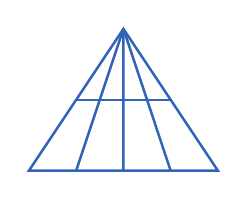
\begin{tikzpicture}[scale=0.6]
\coordinate (A) at (2,3); \coordinate (B) at (0,0); \coordinate (C) at (4,0);
\draw[geo] (A)--(B)--(C)--cycle;
\foreach \x in {1,2,3}{\draw[geo] (A)--(\x,0);}
\draw[geo] (1,1.5)--(3,1.5);
\end{tikzpicture}
\end{minipage}
\end{probbox}
\probsol{
Chưa tính đoạn ngang ở giữa: trên đáy có $5$ điểm, tạo thành $4+3+2+1=10$ hình tam giác có đỉnh A.\par
Đoạn ngang ở giữa cũng có $5$ điểm, tạo thêm $10$ hình tam giác có đỉnh A.\par Tất cả có: $20$ hình tam giác.
\dapso{$20$ hình tam giác.}}
\gap
\begin{probbox}{36}{\stars{1}}
Hình tam giác ABC có $BC=20$ cm. M nằm trên BC sao cho $BM=8$ cm, và hình tam giác ABM có diện tích $40$ cm$^2$. Tính diện tích hình tam giác ABC.
\end{probbox}
\probsol{
Chiều cao chung hạ từ A: $40\times2:8=10$ cm.\par $S_{ABC}=20\times10:2=100$ cm$^2$.
\dapso{$100$ cm$^2$.}}
\gap
\begin{probbox}{37}{\stars{1}}
Hình chữ nhật ABCD có $AB=20$ cm, $AD=12$ cm. M là trung điểm của AB, N là trung điểm của BC. Tính diện tích hình tam giác DMN.
\end{probbox}
\probsol{
Hình chữ nhật: $20\times12=240$ cm$^2$.\par $S_{AMD}=60$, $S_{MBN}=30$, $S_{NCD}=60$ cm$^2$.\par $S_{DMN}=240-60-30-60=90$ cm$^2$.
\dapso{$90$ cm$^2$.}}
\gap
\begin{probbox}{38}{\stars{1}}
Hình vuông ABCD có cạnh $12$ cm, E là một điểm bất kì trên AB. Tính diện tích hình tam giác ECD và tổng diện tích hai hình tam giác AED và EBC.
\end{probbox}
\probsol{
Hình tam giác ECD có đáy $CD=12$ cm và chiều cao $12$ cm.\par $S_{ECD}=72$ cm$^2$.\par Tổng diện tích hai hình tam giác còn lại là $144-72=72$ cm$^2$, dù E ở vị trí nào.
\dapso{Đều bằng $72$ cm$^2$.}}
\gap
\begin{probbox}{39}{\stars{1}}
Một hình tam giác có diện tích $40$ cm$^2$. Nếu gấp độ dài đáy lên ba lần và giảm chiều cao đi một nửa thì diện tích mới là bao nhiêu?
\end{probbox}
\probsol{
Gấp đáy lên ba lần thì diện tích gấp lên ba lần.\par Giảm chiều cao đi một nửa thì diện tích giảm đi một nửa.\par Diện tích mới: $40\times3:2=60$ cm$^2$.
\dapso{$60$ cm$^2$.}}
\gap
\begin{probbox}{40}{\stars{1}}
Tổng độ dài hai cạnh góc vuông của một hình tam giác vuông là $23$ cm, hiệu của chúng là $7$ cm. Tính diện tích hình tam giác đó.
\end{probbox}
\probsol{
Cạnh góc vuông dài hơn: $(23+7):2=15$ cm.\par Cạnh ngắn hơn: $8$ cm.\par Diện tích: $15\times8:2=60$ cm$^2$.
\dapso{$60$ cm$^2$.}}
\gap
\begin{probbox}{41}{\stars{1}}
Hình tam giác ABC có diện tích $90$ cm$^2$. M nằm trên BC sao cho $MC$ gấp đôi $BM$. Tính diện tích các hình tam giác ABM và AMC.
\end{probbox}
\probsol{
$BM=\dfrac13BC$ và $MC=\dfrac23BC$; hai hình tam giác chung chiều cao hạ từ A.\par $S_{ABM}=90:3=30$ cm$^2$.\par $S_{AMC}=60$ cm$^2$.
\dapso{$S_{ABM}=30$ cm$^2$, $S_{AMC}=60$ cm$^2$.}}
\gap
\begin{probbox}{42}{\stars{1}}
Hình tam giác ABC vuông tại A có $AB=12$ cm, $AC=16$ cm. M là trung điểm của AC. So sánh diện tích hai hình tam giác ABM và BMC.
\end{probbox}
\probsol{
$AM=MC=8$ cm; cả hai hình tam giác đều có chiều cao $AB=12$ cm.\par $S_{ABM}=48$ cm$^2$.\par $S_{BMC}=48$ cm$^2$.\par Vậy diện tích hai hình tam giác bằng nhau.
\dapso{Bằng nhau, mỗi hình $48$ cm$^2$.}}
\gap
\begin{probbox}{43}{\stars{1}}
Hình tam giác ABC có $BC=24$ cm và chiều cao $AH=10$ cm. Kéo dài BC về phía C một đoạn $CD=6$ cm. Tính diện tích các hình tam giác ACD và ABD.
\end{probbox}
\probsol{
Các hình tam giác ABC, ACD và ABD đều có chiều cao $AH=10$ cm.\par $S_{ACD}=6\times10:2=30$ cm$^2$.\par $S_{ABD}=30\times10:2=150$ cm$^2$.
\dapso{$30$ cm$^2$ và $150$ cm$^2$.}}
\gap
\begin{probbox}{44}{\stars{1}}
Hai hình tam giác có chiều cao bằng nhau. Đáy của hình thứ nhất bằng $\dfrac23$ đáy của hình thứ hai, và diện tích hình thứ hai lớn hơn diện tích hình thứ nhất $24$ cm$^2$. Tính diện tích mỗi hình.
\end{probbox}
\probsol{
Khi chiều cao bằng nhau, tỉ số diện tích bằng tỉ số độ dài đáy: $S_1=\dfrac23S_2$.\par Hiệu số phần bằng nhau là $3-2=1$ phần, ứng với $24$ cm$^2$.\par $S_1=48$ cm$^2$; $S_2=72$ cm$^2$.
\dapso{$48$ cm$^2$ và $72$ cm$^2$.}}
\gap
\begin{probbox}{45}{\stars{1}}
Một mảnh vườn hình chữ nhật có chiều dài $40$ m, chiều rộng $25$ m. Người ta trồng hoa trên một phần đất hình tam giác có đáy là một chiều dài của mảnh vườn và đỉnh nằm trên cạnh đối diện; phần còn lại trồng cỏ. Tính diện tích mỗi phần.
\end{probbox}
\probsol{
Hình tam giác có đáy $40$ m và chiều cao $25$ m.\par Phần trồng hoa: $500$ m$^2$.\par Mảnh vườn: $1\,000$ m$^2$.\par Phần trồng cỏ: $500$ m$^2$.
\dapso{Trồng hoa $500$ m$^2$, trồng cỏ $500$ m$^2$.}}
\gap
\begin{probbox}{46}{\stars{1}}
Hình tam giác ABC có diện tích $72$ cm$^2$. D nằm trên AB sao cho $AD=\dfrac13AB$; E là trung điểm của AC. Tính diện tích hình tam giác ADE.
\end{probbox}
\probsol{
Nối D với C.\par ADC và ABC chung chiều cao hạ từ C, và $AD=\dfrac13AB$.\par $S_{ADC}=72:3=24$ cm$^2$.\par ADE và ADC chung chiều cao hạ từ D, và $AE=\dfrac12AC$.\par $S_{ADE}=12$ cm$^2$.
\dapso{$12$ cm$^2$.}}
\gap
\begin{probbox}{47}{\stars{1}}
Hình vuông ABCD có cạnh $10$ cm. E là trung điểm của BC, F là trung điểm của CD. Tính diện tích hình tam giác AEF.
\end{probbox}
\probsol{
$S_{ABE}=25$ cm$^2$; $S_{ADF}=25$ cm$^2$.\par $S_{ECF}=5\times5:2=12{,}5$ cm$^2$.\par $S_{AEF}=100-25-25-12{,}5=37{,}5$ cm$^2$.
\dapso{$37{,}5$ cm$^2$.}}
\gap
\begin{probbox}{48}{\stars{2}}
Một hình vuông có đường chéo dài $8$ cm. Tính diện tích hình vuông đó.
\end{probbox}
\probsol{
Một đường chéo chia hình vuông thành hai hình tam giác bằng nhau có chung đáy $8$ cm.\par Hai đường chéo bằng nhau, vuông góc với nhau và cắt nhau tại trung điểm của mỗi đường, nên chiều cao của mỗi hình tam giác là $8:2=4$ cm.\par Mỗi hình tam giác: $8\times4:2=16$ cm$^2$.\par Hình vuông: $32$ cm$^2$.
\dapso{$32$ cm$^2$.}}
\gap
\begin{probbox}{49}{\stars{2}}
Hình tam giác ABC có diện tích $80$ cm$^2$. M là trung điểm của BC, N là trung điểm của AM. Tính diện tích hình tam giác BNC.
\end{probbox}
\probsol{
$S_{ABM}=S_{ACM}=40$ cm$^2$.\par BNM và BAM chung chiều cao hạ từ B và $NM=\dfrac12AM$, nên $S_{BNM}=20$ cm$^2$.\par Tương tự, $S_{CNM}=20$ cm$^2$.\par $S_{BNC}=40$ cm$^2$.
\dapso{$40$ cm$^2$.}}
\gap
\begin{probbox}{50}{\stars{2}}
Hình tam giác ABC có diện tích $120$ cm$^2$. M nằm trên BC sao cho $BM=\dfrac14BC$; N nằm trên AM sao cho $AN=\dfrac23AM$. Tính diện tích các hình tam giác ABN và NBM.
\end{probbox}
\probsol{
$S_{ABM}=120:4=30$ cm$^2$ (chung chiều cao hạ từ A).\par ABN và ABM chung chiều cao hạ từ B, với $AN=\dfrac23AM$.\par $S_{ABN}=20$ cm$^2$.\par $S_{NBM}=10$ cm$^2$.
\dapso{$S_{ABN}=20$ cm$^2$, $S_{NBM}=10$ cm$^2$.}}
\clearpage
\titlehead
\begingroup\setbox0=\vbox{\section*{(*) So sánh diện tích hình tam giác}}\endgroup
\chapterhead{12}{(*) So sánh diện tích hình tam giác}

\shead{Chung chiều cao, so sánh đáy}
\begin{knowbox}
\begin{minipage}[t]{0.6\linewidth}
\begin{itemize}[leftmargin=1.4em,itemsep=3pt]
\item Hai hình tam giác có \textbf{chung chiều cao} thì tỉ số diện tích bằng tỉ số \textbf{độ dài hai đáy}. Chẳng hạn, nếu M nằm trên BC thì
\[\frac{S_{ABM}}{S_{AMC}}=\frac{BM}{MC}.\]
\item Hai hình tam giác có \textbf{chung đáy} thì tỉ số diện tích bằng tỉ số \textbf{hai chiều cao}.
\item Đoạn thẳng nối một đỉnh với \textbf{trung điểm} của cạnh đối diện chia hình tam giác thành hai hình tam giác có diện tích bằng nhau.
\end{itemize}
Để so sánh hai hình tam giác, ta thường đi qua một hình tam giác ``trung gian'' có chung chiều cao với từng hình.
\end{minipage}\hfill
\begin{minipage}[t]{0.36\linewidth}\vspace{4pt}\centering
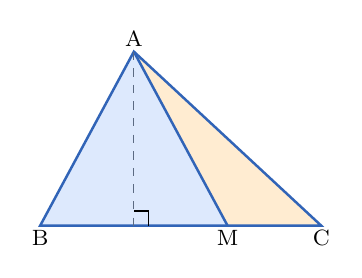
\begin{tikzpicture}[scale=0.85]
\coordinate (B) at (0,0); \coordinate (C) at (4.2,0); \coordinate (A) at (1.4,2.6); \coordinate (M) at (2.8,0); \coordinate (H) at (1.4,0);
\fill[tmBlue!18] (A)--(B)--(M)--cycle; \fill[tmOrange!18] (A)--(M)--(C)--cycle;
\draw[geo] (A)--(B)--(C)--cycle; \draw[geo] (A)--(M);
\draw[dashed,Slate] (A)--(H); \ramark{H}{C}{A}
\node[lbl,above] at (A){A}; \node[lbl,below] at (B){B}; \node[lbl,below] at (C){C}; \node[lbl,below] at (M){M};
\end{tikzpicture}
\end{minipage}
\end{knowbox}
\gap
\begin{exbox}{\ExWord\ 1}
Hình tam giác ABC có diện tích $45$ cm$^2$. Điểm M nằm trên BC sao cho $BM$ gấp đôi $MC$. Tính diện tích các hình tam giác ABM và AMC.
\guide
Hai hình tam giác ABM và AMC chung chiều cao hạ từ A, nên tỉ số diện tích của chúng là $BM:MC=2:1$.\par Nếu $S_{AMC}$ là $1$ phần thì $S_{ABM}$ là $2$ phần và $S_{ABC}$ là $3$ phần.\par
$S_{AMC}=45:3=15$ cm$^2$;\par $S_{ABM}=15\times2=30$ cm$^2$.
\dapso{$30$ cm$^2$ và $15$ cm$^2$.}
\end{exbox}
\gap
\begin{exbox}{\ExWord\ 2}
\begin{minipage}[t]{0.6\linewidth}
Hình tam giác ABC có diện tích $60$ cm$^2$; M là trung điểm của BC và N là trung điểm của AM. Tính diện tích các hình tam giác ABN và BNC.
\end{minipage}\hfill
\begin{minipage}[t]{0.36\linewidth}\vspace{0pt}\centering
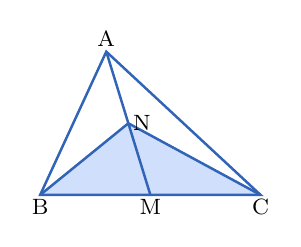
\begin{tikzpicture}[scale=0.7]
\coordinate (B) at (0,0); \coordinate (C) at (4,0); \coordinate (A) at (1.2,2.6); \coordinate (M) at (2,0); \coordinate (N) at (1.6,1.3);
\fill[shade] (B)--(N)--(C)--cycle;
\draw[geo] (A)--(B)--(C)--cycle; \draw[geo] (A)--(M) (B)--(N)--(C);
\node[lbl,above] at (A){A}; \node[lbl,below] at (B){B}; \node[lbl,below] at (C){C}; \node[lbl,below] at (M){M}; \node[lbl,right] at (N){N};
\end{tikzpicture}
\end{minipage}
\guide
M là trung điểm của BC, nên $S_{ABM}=S_{AMC}=60:2=30$ cm$^2$.\par
N là trung điểm của AM, nên $S_{ABN}=S_{NBM}=30:2=15$ cm$^2$; tương tự, $S_{NMC}=15$ cm$^2$.\par
$S_{BNC}=S_{NBM}+S_{NMC}=15+15=30$ cm$^2$.
\dapso{$S_{ABN}=15$ cm$^2$;\par $S_{BNC}=30$ cm$^2$.}
\end{exbox}
\gap
\begin{exbox}{\ExWord\ 3}
Hình tam giác ABC có diện tích $72$ cm$^2$. M nằm trên AB sao cho $AM=\dfrac13AB$, N nằm trên AC sao cho $AN=\dfrac12AC$. Tính diện tích hình tam giác AMN và hình tứ giác BMNC.
\guide
Nối M với C (hình tam giác ``trung gian'' AMC).\par
AMC và ABC chung chiều cao hạ từ C, và $AM=\dfrac13AB$, nên $S_{AMC}=\dfrac13\times72=24$ cm$^2$.\par
AMN và AMC chung chiều cao hạ từ M, và $AN=\dfrac12AC$, nên $S_{AMN}=\dfrac12\times24=12$ cm$^2$.\par
$S_{BMNC}=72-12=60$ cm$^2$.
\dapso{$12$ cm$^2$; $60$ cm$^2$.}
\end{exbox}
\gap
\begin{exbox}{\ExWord\ 4}
Hình vuông ABCD có cạnh $12$ cm; M là trung điểm của AB, N là trung điểm của BC. Tính diện tích hình tam giác DMN.
\guide
Lấy diện tích hình vuông trừ đi diện tích ba hình tam giác vuông ở các góc:\par
$S_{AMD}=6\times12:2=36$;\par $S_{MBN}=6\times6:2=18$;\par $S_{NCD}=6\times12:2=36$ cm$^2$.\par
$S_{DMN}=12\times12-36-18-36=54$ cm$^2$.
\dapso{$54$ cm$^2$.}
\end{exbox}
\dividerbar{Luyện tập}
\begin{probbox}{1}{\relax}
Hình tam giác ABC có diện tích $40$ cm$^2$. M nằm trên BC sao cho $BM=3$ cm và $MC=5$ cm. Tính diện tích các hình tam giác ABM và AMC.
\end{probbox}
\probsol{
Tỉ số diện tích là $3:5$, tổng cộng $8$ phần.\par $S_{ABM}=40:8\times3=15$ cm$^2$; $S_{AMC}=25$ cm$^2$.
\dapso{$15$ cm$^2$ và $25$ cm$^2$.}}
\gap
\begin{probbox}{2}{\relax}
Trong hình tam giác ABC, M là trung điểm của BC và $S_{ABM}=18$ cm$^2$. Tính $S_{ABC}$.
\end{probbox}
\probsol{
$S_{AMC}=S_{ABM}=18$ cm$^2$, nên $S_{ABC}=36$ cm$^2$.
\dapso{$36$ cm$^2$.}}
\gap
\begin{probbox}{3}{\relax}
Hình tam giác ABC có diện tích $90$ cm$^2$. D nằm trên AC sao cho $AD=\dfrac23AC$. Tính diện tích các hình tam giác ABD và BDC.
\end{probbox}
\probsol{
Hai hình tam giác chung chiều cao hạ từ B: $S_{ABD}=\dfrac23\times90=60$ cm$^2$ và $S_{BDC}=30$ cm$^2$.
\dapso{$60$ cm$^2$ và $30$ cm$^2$.}}
\gap
\begin{probbox}{4}{\relax}
Hai điểm M và N chia cạnh BC của hình tam giác ABC thành ba phần bằng nhau $BM=MN=NC$. Biết $S_{AMN}=15$ cm$^2$, tính $S_{ABC}$.
\end{probbox}
\probsol{
ABM, AMN và ANC chung chiều cao và có đáy bằng nhau, nên diện tích của chúng bằng nhau.\par $S_{ABC}=15\times3=45$ cm$^2$.
\dapso{$45$ cm$^2$.}}
\gap
\begin{probbox}{5}{\relax}
Hình tam giác ABC có diện tích $20$ cm$^2$. Kéo dài BC về phía C đến D sao cho $CD=BC$. Tính diện tích các hình tam giác ACD và ABD.
\end{probbox}
\probsol{
ACD và ABC chung chiều cao hạ từ A và có đáy bằng nhau: $S_{ACD}=20$ cm$^2$.\par $S_{ABD}=20+20=40$ cm$^2$.
\dapso{$20$ cm$^2$; $40$ cm$^2$.}}
\gap
\begin{probbox}{6}{\relax}
Hình tam giác ABC có diện tích $60$ cm$^2$; M là trung điểm của BC; N nằm trên AC sao cho $AN=\dfrac13AC$. Tính $S_{MNC}$.
\end{probbox}
\probsol{
$S_{AMC}=60:2=30$ cm$^2$.\par MNC và AMC chung chiều cao hạ từ M và $NC=\dfrac23AC$, nên $S_{MNC}=\dfrac23\times30=20$ cm$^2$.
\dapso{$20$ cm$^2$.}}
\gap
\begin{probbox}{7}{\relax}
Hình tam giác ABC có diện tích $54$ cm$^2$. M nằm trên BC sao cho $BM=\dfrac13BC$; N là trung điểm của AM. Tính diện tích các hình tam giác BNM và ANC.
\end{probbox}
\probsol{
$S_{ABM}=\dfrac13\times54=18$ và $S_{AMC}=36$ cm$^2$.\par N là trung điểm của AM, nên $S_{BNM}=18:2=9$ cm$^2$ và $S_{ANC}=36:2=18$ cm$^2$.
\dapso{$9$ cm$^2$; $18$ cm$^2$.}}
\gap
\begin{probbox}{8}{\relax}
Hình tam giác ABC có diện tích $48$ cm$^2$. M nằm trên AB sao cho $AM=\dfrac23AB$; N nằm trên AC sao cho $AN=\dfrac34AC$. Tính diện tích hình tam giác AMN và hình tứ giác BMNC.
\end{probbox}
\probsol{
$S_{AMC}=\dfrac23\times48=32$ cm$^2$;\par $S_{AMN}=\dfrac34\times32=24$ cm$^2$;\par $S_{BMNC}=48-24=24$ cm$^2$.
\dapso{$24$ cm$^2$; $24$ cm$^2$.}}
\gap
\begin{probbox}{9}{\relax}
Trong hình tam giác ABC, D nằm trên BC sao cho $BD=\dfrac14BC$, và $S_{ABD}=12$ cm$^2$. Tính $S_{ADC}$.
\end{probbox}
\probsol{
$DC=3\times BD$ và hai hình tam giác chung chiều cao hạ từ A, nên $S_{ADC}=12\times3=36$ cm$^2$.
\dapso{$36$ cm$^2$.}}
\gap
\begin{probbox}{10}{\relax}
Hình tam giác ABC có diện tích $60$ cm$^2$. Điểm M trên BC chia BC sao cho $BM:MC=1:2$. Tính diện tích các hình tam giác ABM và AMC.
\end{probbox}
\probsol{
ABM, AMC và ABC chung chiều cao hạ từ A.\par $BM=\dfrac{1}{3}BC$, nên $S_{ABM}=60\times\dfrac{1}{3}=20$ cm$^2$.\par $S_{AMC}=60-20=40$ cm$^2$.
\dapso{$S_{ABM}=20$ cm$^2$, $S_{AMC}=40$ cm$^2$.}}
\gap
\begin{probbox}{11}{\relax}
Hình tam giác ABC có diện tích $84$ cm$^2$. Điểm M trên BC chia BC sao cho $BM:MC=3:4$. Tính diện tích các hình tam giác ABM và AMC.
\end{probbox}
\probsol{
ABM, AMC và ABC chung chiều cao hạ từ A.\par $BM=\dfrac{3}{7}BC$, nên $S_{ABM}=84\times\dfrac{3}{7}=36$ cm$^2$.\par $S_{AMC}=84-36=48$ cm$^2$.
\dapso{$S_{ABM}=36$ cm$^2$, $S_{AMC}=48$ cm$^2$.}}
\gap
\begin{probbox}{12}{\relax}
Hình tam giác ABC có diện tích $100$ cm$^2$. Điểm M trên BC chia BC sao cho $BM:MC=2:3$. Tính diện tích các hình tam giác ABM và AMC.
\end{probbox}
\probsol{
ABM, AMC và ABC chung chiều cao hạ từ A.\par $BM=\dfrac{2}{5}BC$, nên $S_{ABM}=100\times\dfrac{2}{5}=40$ cm$^2$.\par $S_{AMC}=100-40=60$ cm$^2$.
\dapso{$S_{ABM}=40$ cm$^2$, $S_{AMC}=60$ cm$^2$.}}
\gap
\begin{probbox}{13}{\relax}
Hình tam giác ABC có diện tích $72$ cm$^2$. Điểm M trên BC chia BC sao cho $BM:MC=5:1$. Tính diện tích các hình tam giác ABM và AMC.
\end{probbox}
\probsol{
ABM, AMC và ABC chung chiều cao hạ từ A.\par $BM=\dfrac{5}{6}BC$, nên $S_{ABM}=72\times\dfrac{5}{6}=60$ cm$^2$.\par $S_{AMC}=72-60=12$ cm$^2$.
\dapso{$S_{ABM}=60$ cm$^2$, $S_{AMC}=12$ cm$^2$.}}
\gap
\begin{probbox}{14}{\relax}
Hình tam giác ABC có diện tích $45$ cm$^2$. Điểm M trên BC chia BC sao cho $BM:MC=4:5$. Tính diện tích các hình tam giác ABM và AMC.
\end{probbox}
\probsol{
ABM, AMC và ABC chung chiều cao hạ từ A.\par $BM=\dfrac{4}{9}BC$, nên $S_{ABM}=45\times\dfrac{4}{9}=20$ cm$^2$.\par $S_{AMC}=45-20=25$ cm$^2$.
\dapso{$S_{ABM}=20$ cm$^2$, $S_{AMC}=25$ cm$^2$.}}
\gap
\begin{probbox}{15}{\relax}
Trong hình tam giác ABC, điểm M trên BC có $BM=\dfrac{1}{3}BC$. Hình tam giác ABM có diện tích $15$ cm$^2$. Tính diện tích các hình tam giác ABC và AMC.
\end{probbox}
\probsol{
ABM và ABC chung chiều cao hạ từ A, nên $S_{ABM}=\dfrac{1}{3}S_{ABC}$.\par $S_{ABC}=15:\dfrac{1}{3}=45$ cm$^2$.\par $S_{AMC}=45-15=30$ cm$^2$.
\dapso{$S_{ABC}=45$ cm$^2$, $S_{AMC}=30$ cm$^2$.}}
\gap
\begin{probbox}{16}{\relax}
Trong hình tam giác ABC, điểm M trên BC có $BM=\dfrac{2}{5}BC$. Hình tam giác ABM có diện tích $24$ cm$^2$. Tính diện tích các hình tam giác ABC và AMC.
\end{probbox}
\probsol{
ABM và ABC chung chiều cao hạ từ A, nên $S_{ABM}=\dfrac{2}{5}S_{ABC}$.\par $S_{ABC}=24:\dfrac{2}{5}=60$ cm$^2$.\par $S_{AMC}=60-24=36$ cm$^2$.
\dapso{$S_{ABC}=60$ cm$^2$, $S_{AMC}=36$ cm$^2$.}}
\gap
\begin{probbox}{17}{\relax}
Trong hình tam giác ABC, điểm M trên BC có $BM=\dfrac{3}{4}BC$. Hình tam giác ABM có diện tích $21$ cm$^2$. Tính diện tích các hình tam giác ABC và AMC.
\end{probbox}
\probsol{
ABM và ABC chung chiều cao hạ từ A, nên $S_{ABM}=\dfrac{3}{4}S_{ABC}$.\par $S_{ABC}=21:\dfrac{3}{4}=28$ cm$^2$.\par $S_{AMC}=28-21=7$ cm$^2$.
\dapso{$S_{ABC}=28$ cm$^2$, $S_{AMC}=7$ cm$^2$.}}
\gap
\begin{probbox}{18}{\relax}
Trong hình tam giác ABC, điểm M trên BC có $BM=\dfrac{1}{6}BC$. Hình tam giác ABM có diện tích $12$ cm$^2$. Tính diện tích các hình tam giác ABC và AMC.
\end{probbox}
\probsol{
ABM và ABC chung chiều cao hạ từ A, nên $S_{ABM}=\dfrac{1}{6}S_{ABC}$.\par $S_{ABC}=12:\dfrac{1}{6}=72$ cm$^2$.\par $S_{AMC}=72-12=60$ cm$^2$.
\dapso{$S_{ABC}=72$ cm$^2$, $S_{AMC}=60$ cm$^2$.}}
\gap
\begin{probbox}{19}{\relax}
Hình tam giác ABC có diện tích $80$ cm$^2$ và $BC=16$ cm. Điểm M trên BC sao cho hình tam giác ABM có diện tích $30$ cm$^2$. Tính BM.
\end{probbox}
\probsol{
ABM và ABC chung chiều cao hạ từ A, nên tỉ số diện tích bằng tỉ số độ dài hai đáy.\par $\dfrac{BM}{BC}=\dfrac{30}{80}=\dfrac{3}{8}$.\par $BM=16\times\dfrac{3}{8}=6$ cm.
\dapso{$BM=6$ cm.}}
\gap
\begin{probbox}{20}{\relax}
Hình tam giác ABC có diện tích $96$ cm$^2$ và $BC=12$ cm. Điểm M trên BC sao cho hình tam giác ABM có diện tích $36$ cm$^2$. Tính BM.
\end{probbox}
\probsol{
ABM và ABC chung chiều cao hạ từ A, nên tỉ số diện tích bằng tỉ số độ dài hai đáy.\par $\dfrac{BM}{BC}=\dfrac{36}{96}=\dfrac{3}{8}$.\par $BM=12\times\dfrac{3}{8}=4{,}5$ cm.
\dapso{$BM=4{,}5$ cm.}}
\gap
\begin{probbox}{21}{\relax}
Hình tam giác ABC có diện tích $75$ cm$^2$ và $BC=10$ cm. Điểm M trên BC sao cho hình tam giác ABM có diện tích $45$ cm$^2$. Tính BM.
\end{probbox}
\probsol{
ABM và ABC chung chiều cao hạ từ A, nên tỉ số diện tích bằng tỉ số độ dài hai đáy.\par $\dfrac{BM}{BC}=\dfrac{45}{75}=\dfrac{3}{5}$.\par $BM=10\times\dfrac{3}{5}=6$ cm.
\dapso{$BM=6$ cm.}}
\gap
\begin{probbox}{22}{\relax}
Hình tam giác ABC có diện tích $36$ cm$^2$. Kéo dài BC về phía C một đoạn $CD=\dfrac12BC$. Tính diện tích các hình tam giác ACD và ABD.
\end{probbox}
\probsol{
ABC, ACD và ABD chung chiều cao hạ từ A.\par $S_{ACD}=36\times\dfrac{1}{2}=18$ cm$^2$.\par $S_{ABD}=36+18=54$ cm$^2$.
\dapso{$S_{ACD}=18$ cm$^2$, $S_{ABD}=54$ cm$^2$.}}
\gap
\begin{probbox}{23}{\relax}
Hình tam giác ABC có diện tích $50$ cm$^2$. Kéo dài BC về phía C một đoạn $CD=\dfrac25BC$. Tính diện tích các hình tam giác ACD và ABD.
\end{probbox}
\probsol{
ABC, ACD và ABD chung chiều cao hạ từ A.\par $S_{ACD}=50\times\dfrac{2}{5}=20$ cm$^2$.\par $S_{ABD}=50+20=70$ cm$^2$.
\dapso{$S_{ACD}=20$ cm$^2$, $S_{ABD}=70$ cm$^2$.}}
\gap
\begin{probbox}{24}{\relax}
Hình tam giác ABC có diện tích $28$ cm$^2$. Kéo dài BC về phía C một đoạn $CD=2\times BC$. Tính diện tích các hình tam giác ACD và ABD.
\end{probbox}
\probsol{
ABC, ACD và ABD chung chiều cao hạ từ A.\par $S_{ACD}=28\times2=56$ cm$^2$.\par $S_{ABD}=28+56=84$ cm$^2$.
\dapso{$S_{ACD}=56$ cm$^2$, $S_{ABD}=84$ cm$^2$.}}
\gap
\begin{probbox}{25}{\relax}
Hình tam giác ABC có diện tích $60$ cm$^2$. Điểm M trên AB có $AM=\dfrac{1}{2}AB$; điểm N trên AC có $AN=\dfrac{1}{3}AC$. Tính diện tích hình tam giác AMN và hình tứ giác BMNC.
\end{probbox}
\probsol{
Nối M với C.\par AMC và ABC chung chiều cao hạ từ C: $S_{AMC}=60\times\dfrac{1}{2}=30$ cm$^2$.\par AMN và AMC chung chiều cao hạ từ M: $S_{AMN}=30\times\dfrac{1}{3}=10$ cm$^2$.\par $S_{BMNC}=60-10=50$ cm$^2$.
\dapso{$S_{AMN}=10$ cm$^2$, $S_{BMNC}=50$ cm$^2$.}}
\gap
\begin{probbox}{26}{\relax}
Hình tam giác ABC có diện tích $90$ cm$^2$. Điểm M trên AB có $AM=\dfrac{2}{3}AB$; điểm N trên AC có $AN=\dfrac{1}{2}AC$. Tính diện tích hình tam giác AMN và hình tứ giác BMNC.
\end{probbox}
\probsol{
Nối M với C.\par AMC và ABC chung chiều cao hạ từ C: $S_{AMC}=90\times\dfrac{2}{3}=60$ cm$^2$.\par AMN và AMC chung chiều cao hạ từ M: $S_{AMN}=60\times\dfrac{1}{2}=30$ cm$^2$.\par $S_{BMNC}=90-30=60$ cm$^2$.
\dapso{$S_{AMN}=30$ cm$^2$, $S_{BMNC}=60$ cm$^2$.}}
\gap
\begin{probbox}{27}{\relax}
Hình tam giác ABC có diện tích $84$ cm$^2$. Điểm M trên AB có $AM=\dfrac{3}{4}AB$; điểm N trên AC có $AN=\dfrac{2}{3}AC$. Tính diện tích hình tam giác AMN và hình tứ giác BMNC.
\end{probbox}
\probsol{
Nối M với C.\par AMC và ABC chung chiều cao hạ từ C: $S_{AMC}=84\times\dfrac{3}{4}=63$ cm$^2$.\par AMN và AMC chung chiều cao hạ từ M: $S_{AMN}=63\times\dfrac{2}{3}=42$ cm$^2$.\par $S_{BMNC}=84-42=42$ cm$^2$.
\dapso{$S_{AMN}=42$ cm$^2$, $S_{BMNC}=42$ cm$^2$.}}
\gap
\begin{probbox}{28}{\relax}
Hai hình tam giác ABC và DBC có chung đáy BC. Chiều cao hạ từ A là $8$ cm, chiều cao hạ từ D là $6$ cm. Biết $S_{ABC}=40$ cm$^2$, tính $S_{DBC}$.
\end{probbox}
\probsol{
Khi chung đáy, tỉ số diện tích bằng tỉ số hai chiều cao: $\dfrac{S_{DBC}}{S_{ABC}}=\dfrac{6}{8}$.\par $S_{DBC}=40\times6:8=30$ cm$^2$.
\dapso{$30$ cm$^2$.}}
\gap
\begin{probbox}{29}{\relax}
Hai hình tam giác ABC và DBC có chung đáy BC. Chiều cao hạ từ A là $9$ cm, chiều cao hạ từ D là $12$ cm. Biết $S_{ABC}=54$ cm$^2$, tính $S_{DBC}$.
\end{probbox}
\probsol{
Khi chung đáy, tỉ số diện tích bằng tỉ số hai chiều cao: $\dfrac{S_{DBC}}{S_{ABC}}=\dfrac{12}{9}$.\par $S_{DBC}=54\times12:9=72$ cm$^2$.
\dapso{$72$ cm$^2$.}}
\gap
\begin{probbox}{30}{\relax}
Hai hình tam giác ABC và DBC có chung đáy BC. Chiều cao hạ từ A là $10$ cm, chiều cao hạ từ D là $4$ cm. Biết $S_{ABC}=35$ cm$^2$, tính $S_{DBC}$.
\end{probbox}
\probsol{
Khi chung đáy, tỉ số diện tích bằng tỉ số hai chiều cao: $\dfrac{S_{DBC}}{S_{ABC}}=\dfrac{4}{10}$.\par $S_{DBC}=35\times4:10=14$ cm$^2$.
\dapso{$14$ cm$^2$.}}
\dividerbar{Thử thách -- Nâng cao}
\begin{probbox}{31}{\stars{1}}
Hình tam giác ABC có diện tích $64$ cm$^2$; M và N lần lượt là trung điểm của AB và AC. Tính diện tích hình tam giác AMN và hình tứ giác BMNC.
\end{probbox}
\probsol{
$S_{AMC}=64:2=32$ cm$^2$; $S_{AMN}=32:2=16$ cm$^2$.\par $S_{BMNC}=64-16=48$ cm$^2$.
\note{Diện tích hình tam giác AMN bằng $\dfrac14$ diện tích hình tam giác ABC.}
\dapso{$16$ cm$^2$; $48$ cm$^2$.}}
\gap
\begin{probbox}{32}{\stars{1}}
Hình tam giác ABC có diện tích $30$ cm$^2$. Kéo dài AB về phía B đến D sao cho $BD=AB$, kéo dài AC về phía C đến E sao cho $CE=AC$. Tính $S_{ADE}$.
\end{probbox}
\probsol{
$AD=2\times AB$, nên $S_{ADC}=2\times30=60$ cm$^2$.\par $AE=2\times AC$, nên $S_{ADE}=2\times60=120$ cm$^2$.
\dapso{$120$ cm$^2$.}}
\gap
\begin{probbox}{33}{\stars{1}}
Hình tam giác ABC có diện tích $120$ cm$^2$. D nằm trên BC sao cho $BD=2\times DC$; E là trung điểm của AD. Tính $S_{BEC}$.
\end{probbox}
\probsol{
$S_{ABD}=80$ và $S_{ADC}=40$ cm$^2$.\par E là trung điểm của AD, nên $S_{BED}=40$ và $S_{EDC}=20$ cm$^2$.\par
$S_{BEC}=40+20=60$ cm$^2$.
\dapso{$60$ cm$^2$.}}
\gap
\begin{probbox}{34}{\stars{2}}
\begin{minipage}[t]{0.6\linewidth}
Cho hình tam giác ABC, M là trung điểm của BC và I là trung điểm của AM. Đường thẳng BI cắt AC tại N. Chứng tỏ rằng $AN=\dfrac13AC$.
\end{minipage}\hfill
\begin{minipage}[t]{0.36\linewidth}\vspace{0pt}\centering
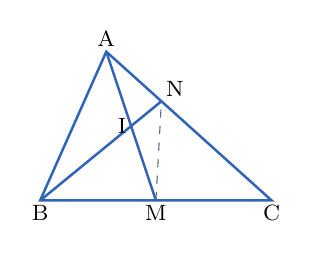
\begin{tikzpicture}[scale=0.7]
\coordinate (B) at (0,0); \coordinate (C) at (4.2,0); \coordinate (A) at (1.2,2.7); \coordinate (M) at (2.1,0); \coordinate (I) at (1.65,1.35); \coordinate (N) at (2.2,1.8);
\draw[geo] (A)--(B)--(C)--cycle; \draw[geo] (A)--(M) (B)--(N);
\draw[dashed,Slate] (M)--(N);
\node[lbl,above] at (A){A}; \node[lbl,below] at (B){B}; \node[lbl,below] at (C){C}; \node[lbl,below] at (M){M}; \node[lbl,left] at (I){I}; \node[lbl,above right] at (N){N};
\end{tikzpicture}
\end{minipage}
\end{probbox}
\probsol{
Nối M với N.\par Vì $AI=IM$ nên $S_{ABI}=S_{MBI}$ và $S_{AIN}=S_{MIN}$.\par Cộng lại: $S_{ABN}=S_{MBN}$.\par
Vì $BM=MC$ nên $S_{MBN}=S_{MNC}$.\par Do đó $S_{BNC}=2\times S_{ABN}$.\par
ABN và CBN chung chiều cao hạ từ B, nên $NC=2\times AN$, tức là\par $AN=\dfrac13AC$.
\dapso{Đã chứng tỏ được điều phải chứng minh.}}
\gap
\begin{probbox}{35}{\stars{2}}
Hình tam giác ABC có diện tích $90$ cm$^2$. M nằm trên BC sao cho $BM=\dfrac13BC$, N nằm trên CA sao cho $CN=\dfrac13CA$, và P nằm trên AB sao cho $AP=\dfrac13AB$. Tính $S_{MNP}$.
\end{probbox}
\probsol{
Hình tam giác APN: $S_{APC}=\dfrac13\times90=30$; $AN=\dfrac23AC$, nên $S_{APN}=\dfrac23\times30=20$ cm$^2$.\par
Tương tự, $S_{BMP}=20$ và $S_{CNM}=20$ cm$^2$.\par Vậy $S_{MNP}=90-3\times20=30$ cm$^2$.
\dapso{$30$ cm$^2$.}}
\gap
\begin{probbox}{36}{\stars{1}}
Hình tam giác ABC có diện tích $60$ cm$^2$. Điểm M trên BC có $BM=\dfrac{1}{3}BC$; điểm N trên AM có $AN=\dfrac{1}{2}AM$. Tính diện tích các hình tam giác ABN, NBM và ANC.
\end{probbox}
\probsol{
$S_{ABM}=60\times\dfrac{1}{3}=20$ cm$^2$; $S_{AMC}=40$ cm$^2$.\par ABN và ABM chung chiều cao hạ từ B: $S_{ABN}=20\times\dfrac{1}{2}=10$ cm$^2$.\par $S_{NBM}=20-10=10$ cm$^2$.\par ANC và AMC chung chiều cao hạ từ C: $S_{ANC}=40\times\dfrac{1}{2}=20$ cm$^2$.
\dapso{$S_{ABN}=10$, $S_{NBM}=10$, $S_{ANC}=20$ (cm$^2$).}}
\gap
\begin{probbox}{37}{\stars{1}}
Hình tam giác ABC có diện tích $96$ cm$^2$. Điểm M trên BC có $BM=\dfrac{1}{4}BC$; điểm N trên AM có $AN=\dfrac{2}{3}AM$. Tính diện tích các hình tam giác ABN, NBM và ANC.
\end{probbox}
\probsol{
$S_{ABM}=96\times\dfrac{1}{4}=24$ cm$^2$; $S_{AMC}=72$ cm$^2$.\par ABN và ABM chung chiều cao hạ từ B: $S_{ABN}=24\times\dfrac{2}{3}=16$ cm$^2$.\par $S_{NBM}=24-16=8$ cm$^2$.\par ANC và AMC chung chiều cao hạ từ C: $S_{ANC}=72\times\dfrac{2}{3}=48$ cm$^2$.
\dapso{$S_{ABN}=16$, $S_{NBM}=8$, $S_{ANC}=48$ (cm$^2$).}}
\gap
\begin{probbox}{38}{\stars{1}}
Hình tam giác ABC có diện tích $150$ cm$^2$. Điểm M trên BC có $BM=\dfrac{2}{5}BC$; điểm N trên AM có $AN=\dfrac{3}{5}AM$. Tính diện tích các hình tam giác ABN, NBM và ANC.
\end{probbox}
\probsol{
$S_{ABM}=150\times\dfrac{2}{5}=60$ cm$^2$; $S_{AMC}=90$ cm$^2$.\par ABN và ABM chung chiều cao hạ từ B: $S_{ABN}=60\times\dfrac{3}{5}=36$ cm$^2$.\par $S_{NBM}=60-36=24$ cm$^2$.\par ANC và AMC chung chiều cao hạ từ C: $S_{ANC}=90\times\dfrac{3}{5}=54$ cm$^2$.
\dapso{$S_{ABN}=36$, $S_{NBM}=24$, $S_{ANC}=54$ (cm$^2$).}}
\gap
\begin{probbox}{39}{\stars{1}}
Điểm M trên AB có $AM=\dfrac{1}{2}AB$ và điểm N trên AC có $AN=\dfrac{2}{5}AC$. Hình tam giác AMN có diện tích $10$ cm$^2$. Tính diện tích hình tam giác ABC.
\end{probbox}
\probsol{
Nối M với C.\par AMN và AMC chung chiều cao hạ từ M: $S_{AMC}=10:\dfrac{2}{5}=25$ cm$^2$.\par AMC và ABC chung chiều cao hạ từ C: $S_{ABC}=25:\dfrac{1}{2}=50$ cm$^2$.
\dapso{$50$ cm$^2$.}}
\gap
\begin{probbox}{40}{\stars{1}}
Điểm M trên AB có $AM=\dfrac{3}{4}AB$ và điểm N trên AC có $AN=\dfrac{2}{3}AC$. Hình tam giác AMN có diện tích $18$ cm$^2$. Tính diện tích hình tam giác ABC.
\end{probbox}
\probsol{
Nối M với C.\par AMN và AMC chung chiều cao hạ từ M: $S_{AMC}=18:\dfrac{2}{3}=27$ cm$^2$.\par AMC và ABC chung chiều cao hạ từ C: $S_{ABC}=27:\dfrac{3}{4}=36$ cm$^2$.
\dapso{$36$ cm$^2$.}}
\gap
\begin{probbox}{41}{\stars{1}}
Hình tam giác ABC có diện tích $12$ cm$^2$. Kéo dài AB về phía B một đoạn $BD=AB$ và kéo dài AC về phía C một đoạn $CE=2\times AC$. Tính diện tích hình tam giác ADE.
\end{probbox}
\probsol{
$AD=2\times AB$, $AE=3\times AC$.\par Nối D với C.\par ADC và ABC chung chiều cao hạ từ C: $S_{ADC}=12\times2=24$ cm$^2$.\par ADE và ADC chung chiều cao hạ từ D: $S_{ADE}=24\times3=72$ cm$^2$.
\dapso{$72$ cm$^2$.}}
\gap
\begin{probbox}{42}{\stars{1}}
Hình tam giác ABC có diện tích $15$ cm$^2$. Kéo dài AB về phía B một đoạn $BD=2\times AB$ và kéo dài AC về phía C một đoạn $CE=2\times AC$. Tính diện tích hình tam giác ADE.
\end{probbox}
\probsol{
$AD=3\times AB$, $AE=3\times AC$.\par Nối D với C.\par ADC và ABC chung chiều cao hạ từ C: $S_{ADC}=15\times3=45$ cm$^2$.\par ADE và ADC chung chiều cao hạ từ D: $S_{ADE}=45\times3=135$ cm$^2$.
\dapso{$135$ cm$^2$.}}
\gap
\begin{probbox}{43}{\stars{2}}
Hình tam giác ABC có diện tích $80$ cm$^2$. Các điểm M, N, P lần lượt nằm trên AB, BC, CA sao cho $AM=\dfrac{1}{4}AB$, $BN=\dfrac{1}{4}BC$, $CP=\dfrac{1}{4}CA$. Tính diện tích hình tam giác MNP.
\end{probbox}
\probsol{
Trong hình tam giác AMP: $AM=\dfrac{1}{4}AB$, $AP=\dfrac{3}{4}AC$.\par Làm như trên (nối M với C): $S_{AMP}=80\times\dfrac{1}{4}\times\dfrac{3}{4}=15$ cm$^2$.\par Tương tự, $S_{BNM}=S_{CPN}=15$ cm$^2$.\par $S_{MNP}=80-3\times15=35$ cm$^2$.
\dapso{$35$ cm$^2$.}}
\gap
\begin{probbox}{44}{\stars{2}}
Hình tam giác ABC có diện tích $72$ cm$^2$. Các điểm M, N, P lần lượt nằm trên AB, BC, CA sao cho $AM=\dfrac{1}{3}AB$, $BN=\dfrac{1}{3}BC$, $CP=\dfrac{1}{3}CA$. Tính diện tích hình tam giác MNP.
\end{probbox}
\probsol{
Trong hình tam giác AMP: $AM=\dfrac{1}{3}AB$, $AP=\dfrac{2}{3}AC$.\par Làm như trên (nối M với C): $S_{AMP}=72\times\dfrac{1}{3}\times\dfrac{2}{3}=16$ cm$^2$.\par Tương tự, $S_{BNM}=S_{CPN}=16$ cm$^2$.\par $S_{MNP}=72-3\times16=24$ cm$^2$.
\dapso{$24$ cm$^2$.}}
\gap
\begin{probbox}{45}{\stars{1}}
Trong hình tam giác ABC, điểm M trên BC có $BM:MC=3:1$. Diện tích hình tam giác ABM lớn hơn diện tích hình tam giác AMC là $20$ cm$^2$. Tính diện tích hình tam giác ABC.
\end{probbox}
\probsol{
ABM và AMC chung chiều cao hạ từ A, nên $S_{ABM}:S_{AMC}=3:1$.\par Hiệu $2$ phần ứng với $20$ cm$^2$; một phần là $10$ cm$^2$.\par $S_{ABC}=10\times4=40$ cm$^2$.
\dapso{$40$ cm$^2$.}}
\gap
\begin{probbox}{46}{\stars{1}}
Trong hình tam giác ABC, điểm M trên BC có $BM:MC=5:2$. Diện tích hình tam giác ABM lớn hơn diện tích hình tam giác AMC là $24$ cm$^2$. Tính diện tích hình tam giác ABC.
\end{probbox}
\probsol{
ABM và AMC chung chiều cao hạ từ A, nên $S_{ABM}:S_{AMC}=5:2$.\par Hiệu $3$ phần ứng với $24$ cm$^2$; một phần là $8$ cm$^2$.\par $S_{ABC}=8\times7=56$ cm$^2$.
\dapso{$56$ cm$^2$.}}
\gap
\begin{probbox}{47}{\stars{1}}
Hình chữ nhật ABCD có $AB=24$ cm, $BC=16$ cm. Điểm M trên AB có $AM=8$ cm; điểm N trên BC có $BN=6$ cm. Tính diện tích hình tam giác DMN.
\end{probbox}
\probsol{
$S_{ABCD}=24\times16=384$ cm$^2$.\par $S_{AMD}=64$, $S_{MBN}=48$, $S_{NCD}=120$ cm$^2$.\par $S_{DMN}=384-64-48-120=152$ cm$^2$.
\dapso{$152$ cm$^2$.}}
\gap
\begin{probbox}{48}{\stars{1}}
Hình chữ nhật ABCD có $AB=30$ cm, $BC=20$ cm. Điểm M trên AB có $AM=12$ cm; điểm N trên BC có $BN=10$ cm. Tính diện tích hình tam giác DMN.
\end{probbox}
\probsol{
$S_{ABCD}=30\times20=600$ cm$^2$.\par $S_{AMD}=120$, $S_{MBN}=90$, $S_{NCD}=150$ cm$^2$.\par $S_{DMN}=600-120-90-150=240$ cm$^2$.
\dapso{$240$ cm$^2$.}}
\gap
\begin{probbox}{49}{\stars{1}}
Hình chữ nhật ABCD có $AB=18$ cm, $BC=12$ cm. Điểm M trên AB có $AM=6$ cm; điểm N trên BC có $BN=4$ cm. Tính diện tích hình tam giác DMN.
\end{probbox}
\probsol{
$S_{ABCD}=18\times12=216$ cm$^2$.\par $S_{AMD}=36$, $S_{MBN}=24$, $S_{NCD}=72$ cm$^2$.\par $S_{DMN}=216-36-24-72=84$ cm$^2$.
\dapso{$84$ cm$^2$.}}
\gap
\begin{probbox}{50}{\stars{1}}
Hình tam giác ABC có $BC=16$ cm. Kéo dài BC về phía C thêm $5$ cm thì được một hình tam giác có diện tích lớn hơn diện tích hình tam giác ABC là $25$ cm$^2$. Tính diện tích hình tam giác ABC.
\end{probbox}
\probsol{
Phần tăng thêm là hình tam giác có đáy $5$ cm và có cùng chiều cao hạ từ A.\par Chiều cao: $25\times2:5=10$ cm.\par $S_{ABC}=16\times10:2=80$ cm$^2$.
\dapso{$80$ cm$^2$.}}
\clearpage
\titlehead
\begingroup\setbox0=\vbox{\section*{Hình thang và diện tích hình thang}}\endgroup
\chapterhead{13}{Hình thang và diện tích hình thang}

\shead{Hai đáy song song}
\begin{knowbox}
\begin{minipage}[t]{0.6\linewidth}
\textbf{Hình thang} là tứ giác có \emph{một cặp cạnh đối diện song song}: \textbf{đáy lớn} và \textbf{đáy bé}. Hai cạnh còn lại là \textbf{cạnh bên}. Hình thang có một cạnh bên vuông góc với hai đáy gọi là \textbf{hình thang vuông}.\par
\smallskip
\textbf{Chiều cao} là khoảng cách giữa hai đáy.
\[S=\frac{(a+b)\times h}{2}\qquad h=\frac{S\times2}{a+b}\qquad a+b=\frac{S\times2}{h}\]
\textbf{Hai đường chéo.} Trong hình thang ABCD (AB song song với CD), hai tam giác ACD và BCD có chung đáy CD và chiều cao bằng nhau, nên $S_{ACD}=S_{BCD}$; bớt đi phần chung ta được $S_{AOD}=S_{BOC}$.
\end{minipage}\hfill
\begin{minipage}[t]{0.36\linewidth}\vspace{4pt}\centering
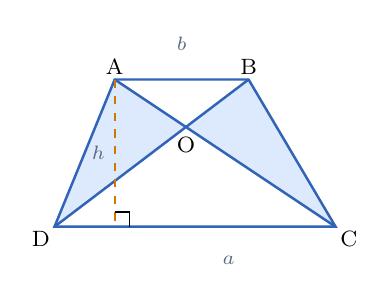
\begin{tikzpicture}[scale=0.85]
\coordinate (D) at (0,0); \coordinate (C) at (4.2,0); \coordinate (A) at (0.9,2.2); \coordinate (B) at (2.9,2.2); \coordinate (H) at (0.9,0);
\coordinate (O) at (intersection of A--C and B--D);
\fill[tmBlue!18] (A)--(O)--(D)--cycle; \fill[tmBlue!18] (B)--(O)--(C)--cycle;
\draw[geo] (A)--(B)--(C)--(D)--cycle; \draw[geo] (A)--(C) (B)--(D);
\draw[dashed,tmOrange!80!black,line width=0.7pt] (A)--(H); \ramark{H}{C}{A}
\node[lbl,above] at (A){A}; \node[lbl,above] at (B){B}; \node[lbl,below right] at (C){C}; \node[lbl,below left] at (D){D}; \node[lbl,below=2pt] at (O){O};
\node[dim,left] at (0.9,1.1){$h$}; \node[dim,above=7pt] at (1.9,2.2){$b$}; \node[dim,below=7pt] at (2.6,0){$a$};
\end{tikzpicture}
\end{minipage}
\end{knowbox}
\gap
\begin{exbox}{\ExWord\ 1}
Tính diện tích hình thang có hai đáy là $12$ cm và $8$ cm, chiều cao $5$ cm.
\guide
$S=(12+8)\times5:2=50$ cm$^2$.
\dapso{$50$ cm$^2$.}
\end{exbox}
\gap
\begin{exbox}{\ExWord\ 2}
Một thửa ruộng hình thang có đáy lớn $120$ m; đáy bé bằng $\dfrac23$ đáy lớn, chiều cao bằng trung bình cộng của hai đáy. Cứ $100$ m$^2$ thu hoạch được $64$ kg thóc. Hỏi thửa ruộng đó thu hoạch được bao nhiêu ki-lô-gam thóc?
\guide
Đáy bé: $120\times\dfrac23=80$ m.\par Chiều cao: $(120+80):2=100$ m.\par
Diện tích: $(120+80)\times100:2=10\,000$ m$^2$.\par Số thóc: $64\times(10\,000:100)=6\,400$ kg.
\dapso{$6\,400$ kg.}
\end{exbox}
\gap
\begin{exbox}{\ExWord\ 3}
Một hình thang có diện tích $60$ cm$^2$, chiều cao $6$ cm; đáy lớn hơn đáy bé $4$ cm. Tính độ dài mỗi đáy.
\guide
Tổng hai đáy: $60\times2:6=20$ cm.\par Đây là bài toán tổng -- hiệu: đáy lớn $(20+4):2=12$ cm, đáy bé $8$ cm.
\dapso{$12$ cm và $8$ cm.}
\end{exbox}
\gap
\begin{exbox}{\ExWord\ 4}
Hình thang ABCD có đáy bé $AB=6$ cm, đáy lớn $CD=9$ cm và chiều cao $4$ cm. Tính diện tích các tam giác ABD và BCD, và chứng tỏ rằng $S_{AOD}=S_{BOC}$ (O là giao điểm của hai đường chéo).
\guide
Cả hai tam giác đều có chiều cao bằng chiều cao hình thang: $S_{ABD}=6\times4:2=12$ cm$^2$ và $S_{BCD}=9\times4:2=18$ cm$^2$.\par
$S_{ACD}=S_{BCD}=18$ cm$^2$ (chung đáy CD, cùng chiều cao).\par Bớt đi phần chung của chúng là tam giác OCD, ta được $S_{AOD}=S_{BOC}$.
\dapso{$12$ cm$^2$; $18$ cm$^2$.}
\end{exbox}
\dividerbar{Luyện tập}
\begin{probbox}{1}{\relax}
Tính diện tích hình thang có hai đáy $a$, $b$ và chiều cao $h$:
\begin{cols2}
\pa{a} $a=14$ cm, $b=6$ cm, $h=7$ cm; & \pa{b} $a=2{,}8$ m, $b=1{,}6$ m, $h=0{,}5$ m;\\
\pa{c} $a=\dfrac34$ dm, $b=\dfrac12$ dm, $h=\dfrac23$ dm; & \pa{d} $a=1{,}5$ dm, $b=9$ cm, $h=8$ cm.
\end{cols2}
\end{probbox}
\probsol{
\pa{a} $(14+6)\times7:2=70$ cm$^2$.\par \pa{b} $(2{,}8+1{,}6)\times0{,}5:2=1{,}1$ m$^2$.\par \pa{c} $\left(\dfrac34+\dfrac12\right)\times\dfrac23:2=\dfrac5{12}$ dm$^2$.\par \pa{d} $1{,}5$ dm $=15$ cm; $(15+9)\times8:2=96$ cm$^2$.
\dapso{$70$ cm$^2$; $1{,}1$ m$^2$; $\dfrac5{12}$ dm$^2$; $96$ cm$^2$.}}
\gap
\begin{probbox}{2}{\relax}
Một hình thang vuông có hai đáy là $10$ cm và $7$ cm, cạnh bên vuông góc với hai đáy dài $6$ cm. Tính diện tích hình thang đó.
\end{probbox}
\probsol{
Cạnh bên vuông góc với hai đáy chính là chiều cao: $S=(10+7)\times6:2=51$ cm$^2$.
\dapso{$51$ cm$^2$.}}
\gap
\begin{probbox}{3}{\relax}
Một hình thang có diện tích $72$ cm$^2$, hai đáy là $10$ cm và $14$ cm. Tính chiều cao của hình thang.
\end{probbox}
\probsol{
$h=72\times2:(10+14)=6$ cm.
\dapso{$6$ cm.}}
\gap
\begin{probbox}{4}{\relax}
Một hình thang có diện tích $45$ m$^2$, chiều cao $5$ m và đáy bé $7$ m. Tính đáy lớn.
\end{probbox}
\probsol{
Tổng hai đáy: $45\times2:5=18$ m.\par Đáy lớn: $18-7=11$ m.
\dapso{$11$ m.}}
\gap
\begin{probbox}{5}{\relax}
Một thửa ruộng hình thang có hai đáy là $60$ m và $40$ m, chiều cao $30$ m. Cứ $100$ m$^2$ thu hoạch được $70$ kg thóc. Hỏi thửa ruộng đó thu hoạch được bao nhiêu ki-lô-gam thóc?
\end{probbox}
\probsol{
Diện tích: $(60+40)\times30:2=1\,500$ m$^2$.\par Số thóc: $70\times15=1\,050$ kg.
\dapso{$1\,050$ kg.}}
\gap
\begin{probbox}{6}{\relax}
Một hình thang có tổng hai đáy là $48$ cm; đáy bé bằng $\dfrac35$ đáy lớn, chiều cao bằng $\dfrac14$ đáy lớn. Tính diện tích hình thang.
\end{probbox}
\probsol{
Đáy lớn: $48:(3+5)\times5=30$ cm; chiều cao: $30\times\dfrac14=7{,}5$ cm.\par $S=48\times7{,}5:2=180$ cm$^2$.
\dapso{$180$ cm$^2$.}}
\gap
\begin{probbox}{7}{\relax}
Một hình thang có hai đáy là $25$ cm và $15$ cm. Nếu kéo dài đáy lớn thêm $5$ cm thì diện tích tăng thêm $20$ cm$^2$. Tính diện tích hình thang ban đầu.
\end{probbox}
\probsol{
Phần tăng thêm là một tam giác có đáy $5$ cm và chiều cao bằng chiều cao hình thang: $h=20\times2:5=8$ cm.\par $S=(25+15)\times8:2=160$ cm$^2$.
\dapso{$160$ cm$^2$.}}
\gap
\begin{probbox}{8}{\relax}
Hình chữ nhật ABCD có $AB=20$ cm và $BC=12$ cm. Điểm M nằm trên AB sao cho $AM=8$ cm. Tính diện tích hình thang MBCD.
\end{probbox}
\probsol{
Hình thang MBCD có hai đáy $MB=12$ cm và $CD=20$ cm, chiều cao $BC=12$ cm: $S=(12+20)\times12:2=192$ cm$^2$.\par
\emph{Cách khác:} $20\times12-8\times12:2=240-48=192$ cm$^2$.
\dapso{$192$ cm$^2$.}}
\gap
\begin{probbox}{9}{\relax}
Hình thang ABCD có $AB=4$ cm, $CD=10$ cm và chiều cao $6$ cm. Tính diện tích các tam giác ABC và ACD.
\end{probbox}
\probsol{
$S_{ABC}=4\times6:2=12$ cm$^2$;\par $S_{ACD}=10\times6:2=30$ cm$^2$.\par \emph{Thử lại:} $12+30=42=(4+10)\times6:2$.
\dapso{$12$ cm$^2$; $30$ cm$^2$.}}
\gap
\begin{probbox}{10}{\relax}
Tính diện tích hình thang có hai đáy là $15$ cm và $9$ cm, chiều cao $6$ cm.
\end{probbox}
\probsol{
$S=(15+9)\times6:2=72$ cm$^2$.
\dapso{$72$ cm$^2$.}}
\gap
\begin{probbox}{11}{\relax}
Tính diện tích hình thang có hai đáy là $6{,}5$ cm và $3{,}5$ cm, chiều cao $4{,}2$ cm.
\end{probbox}
\probsol{
$S=(6{,}5+3{,}5)\times4{,}2:2=21$ cm$^2$.
\dapso{$21$ cm$^2$.}}
\gap
\begin{probbox}{12}{\relax}
Tính diện tích hình thang có hai đáy là $\dfrac34$ m và $\dfrac12$ m, chiều cao $\dfrac23$ m.
\end{probbox}
\probsol{
$S=\left(\dfrac34+\dfrac12\right)\times\dfrac23:2=\dfrac54\times\dfrac23:2=\dfrac5{12}$ m$^2$.
\dapso{$\dfrac5{12}$ m$^2$.}}
\gap
\begin{probbox}{13}{\relax}
Tính diện tích hình thang có hai đáy là $14$ dm và $10$ dm, chiều cao $7{,}5$ dm.
\end{probbox}
\probsol{
$S=(14+10)\times7{,}5:2=90$ dm$^2$.
\dapso{$90$ dm$^2$.}}
\gap
\begin{probbox}{14}{\relax}
Tính diện tích hình thang có hai đáy là $1{,}2$ m và $80$ cm, chiều cao $5$ dm.
\end{probbox}
\probsol{
Đổi ra đề-xi-mét: $1{,}2$ m $=12$ dm; $80$ cm $=8$ dm.\par $S=(12+8)\times5:2=50$ dm$^2$.
\dapso{$50$ dm$^2$.}}
\gap
\begin{probbox}{15}{\relax}
Một hình thang có diện tích $84$ cm$^2$, hai đáy là $16$ cm và $12$ cm. Tính chiều cao của hình thang.
\end{probbox}
\probsol{
Chiều cao $=$ diện tích $\times2\,:$ tổng hai đáy.\par $h=84\times2:(16+12)=6$ cm.
\dapso{$6$ cm.}}
\gap
\begin{probbox}{16}{\relax}
Một hình thang có diện tích $45$ cm$^2$, hai đáy là $8{,}5$ cm và $6{,}5$ cm. Tính chiều cao của hình thang.
\end{probbox}
\probsol{
Chiều cao $=$ diện tích $\times2\,:$ tổng hai đáy.\par $h=45\times2:(8{,}5+6{,}5)=6$ cm.
\dapso{$6$ cm.}}
\gap
\begin{probbox}{17}{\relax}
Một hình thang có diện tích $150$ cm$^2$, hai đáy là $23$ cm và $17$ cm. Tính chiều cao của hình thang.
\end{probbox}
\probsol{
Chiều cao $=$ diện tích $\times2\,:$ tổng hai đáy.\par $h=150\times2:(23+17)=7{,}5$ cm.
\dapso{$7{,}5$ cm.}}
\gap
\begin{probbox}{18}{\relax}
Một hình thang có diện tích $96$ cm$^2$, chiều cao $8$ cm và đáy bé $10$ cm. Tính đáy lớn.
\end{probbox}
\probsol{
Tổng hai đáy: $96\times2:8=24$ cm.\par Đáy lớn: $24-10=14$ cm.
\dapso{$14$ cm.}}
\gap
\begin{probbox}{19}{\relax}
Một hình thang có diện tích $63$ cm$^2$, chiều cao $7$ cm và đáy bé $7{,}5$ cm. Tính đáy lớn.
\end{probbox}
\probsol{
Tổng hai đáy: $63\times2:7=18$ cm.\par Đáy lớn: $18-7{,}5=10{,}5$ cm.
\dapso{$10{,}5$ cm.}}
\gap
\begin{probbox}{20}{\relax}
Một hình thang có diện tích $110$ cm$^2$, chiều cao $10$ cm và đáy bé $9$ cm. Tính đáy lớn.
\end{probbox}
\probsol{
Tổng hai đáy: $110\times2:10=22$ cm.\par Đáy lớn: $22-9=13$ cm.
\dapso{$13$ cm.}}
\gap
\begin{probbox}{21}{\relax}
Một thửa ruộng hình thang có hai đáy là $80$ m và $50$ m, chiều cao $40$ m. Cứ $100$ m$^2$ thu hoạch được $65$ kg thóc. Hỏi cả thửa ruộng thu hoạch được bao nhiêu ki-lô-gam thóc?
\end{probbox}
\probsol{
Diện tích: $(80+50)\times40:2=2\,600$ m$^2$.\par Số thóc: $2\,600:100\times65=1\,690$ kg.
\dapso{$1\,690$ kg.}}
\gap
\begin{probbox}{22}{\relax}
Một thửa ruộng hình thang có hai đáy là $150$ m và $90$ m, chiều cao $60$ m. Cứ $100$ m$^2$ thu hoạch được $60$ kg thóc. Hỏi cả thửa ruộng thu hoạch được bao nhiêu ki-lô-gam thóc?
\end{probbox}
\probsol{
Diện tích: $(150+90)\times60:2=7\,200$ m$^2$.\par Số thóc: $7\,200:100\times60=4\,320$ kg.
\dapso{$4\,320$ kg.}}
\gap
\begin{probbox}{23}{\relax}
Một hình thang có tổng hai đáy là $36$ cm, hiệu hai đáy là $8$ cm; chiều cao $10$ cm. Tính mỗi đáy và diện tích hình thang.
\end{probbox}
\probsol{
Đáy lớn: $(36+8):2=22$ cm; đáy bé: $14$ cm.\par Diện tích: $36\times10:2=180$ cm$^2$.
\dapso{Hai đáy $22$ cm và $14$ cm; $180$ cm$^2$.}}
\gap
\begin{probbox}{24}{\relax}
Một hình thang có tổng hai đáy là $50$ cm, hiệu hai đáy là $14$ cm; chiều cao $12$ cm. Tính mỗi đáy và diện tích hình thang.
\end{probbox}
\probsol{
Đáy lớn: $(50+14):2=32$ cm; đáy bé: $18$ cm.\par Diện tích: $50\times12:2=300$ cm$^2$.
\dapso{Hai đáy $32$ cm và $18$ cm; $300$ cm$^2$.}}
\gap
\begin{probbox}{25}{\relax}
Một mảnh đất hình thang có đáy lớn $60$ m; đáy bé bằng $\dfrac{2}{3}$ đáy lớn và chiều cao bằng $\dfrac{1}{2}$ đáy lớn. Tính diện tích mảnh đất.
\end{probbox}
\probsol{
Đáy bé: $60\times\dfrac{2}{3}=40$ m.\par Chiều cao: $60\times\dfrac{1}{2}=30$ m.\par Diện tích: $(60+40)\times30:2=1\,500$ m$^2$.
\dapso{$1\,500$ m$^2$.}}
\gap
\begin{probbox}{26}{\relax}
Một mảnh đất hình thang có đáy lớn $48$ m; đáy bé bằng $\dfrac{3}{4}$ đáy lớn và chiều cao bằng $\dfrac{5}{8}$ đáy lớn. Tính diện tích mảnh đất.
\end{probbox}
\probsol{
Đáy bé: $48\times\dfrac{3}{4}=36$ m.\par Chiều cao: $48\times\dfrac{5}{8}=30$ m.\par Diện tích: $(48+36)\times30:2=1\,260$ m$^2$.
\dapso{$1\,260$ m$^2$.}}
\gap
\begin{probbox}{27}{\relax}
Hình thang ABCD có góc A và góc D vuông, $AB=9$ cm, $CD=15$ cm và $AD=8$ cm. Tính diện tích hình thang.
\end{probbox}
\probsol{
AD vuông góc với cả hai đáy nên AD là chiều cao.\par $S=(9+15)\times8:2=96$ cm$^2$.
\dapso{$96$ cm$^2$.}}
\gap
\begin{probbox}{28}{\relax}
Hình thang ABCD có góc A và góc D vuông, $AB=4{,}5$ cm, $CD=7{,}5$ cm và $AD=6$ cm. Tính diện tích hình thang.
\end{probbox}
\probsol{
AD vuông góc với cả hai đáy nên AD là chiều cao.\par $S=(4{,}5+7{,}5)\times6:2=36$ cm$^2$.
\dapso{$36$ cm$^2$.}}
\gap
\begin{probbox}{29}{\relax}
Hình chữ nhật ABCD có $AB=25$ cm và $BC=14$ cm. Điểm M trên AB có $AM=9$ cm. Tính diện tích hình thang MBCD và tam giác AMD.
\end{probbox}
\probsol{
Hình thang MBCD có hai đáy $MB=16$ cm và $CD=25$ cm, chiều cao $BC=14$ cm.\par $S_{MBCD}=(16+25)\times14:2=287$ cm$^2$.\par $S_{AMD}=9\times14:2=63$ cm$^2$.
\dapso{$S_{MBCD}=287$ cm$^2$, $S_{AMD}=63$ cm$^2$.}}
\gap
\begin{probbox}{30}{\relax}
Hình chữ nhật ABCD có $AB=30$ cm và $BC=16$ cm. Điểm M trên AB có $AM=12$ cm. Tính diện tích hình thang MBCD và tam giác AMD.
\end{probbox}
\probsol{
Hình thang MBCD có hai đáy $MB=18$ cm và $CD=30$ cm, chiều cao $BC=16$ cm.\par $S_{MBCD}=(18+30)\times16:2=384$ cm$^2$.\par $S_{AMD}=12\times16:2=96$ cm$^2$.
\dapso{$S_{MBCD}=384$ cm$^2$, $S_{AMD}=96$ cm$^2$.}}
\dividerbar{Thử thách -- Nâng cao}
\begin{probbox}{31}{\stars{1}}
Một hình thang có hai đáy là $12$ cm và $18$ cm. Nếu kéo dài đáy bé thêm $6$ cm thì được một hình chữ nhật và diện tích tăng thêm $27$ cm$^2$. Tính diện tích hình thang.
\end{probbox}
\probsol{
Phần tăng thêm là một tam giác có một cạnh $6$ cm và chiều cao bằng chiều cao hình thang: $h=27\times2:6=9$ cm.\par $S=(12+18)\times9:2=135$ cm$^2$.
\dapso{$135$ cm$^2$.}}
\gap
\begin{probbox}{32}{\stars{1}}
Một thửa ruộng hình thang có tổng hai đáy là $140$ m, đáy lớn hơn đáy bé $20$ m. Nếu kéo dài mỗi đáy thêm $10$ m thì diện tích tăng thêm $500$ m$^2$. Tính diện tích ban đầu và độ dài mỗi đáy.
\end{probbox}
\probsol{
Hai đáy tăng tổng cộng $20$ m, nên $h=500\times2:20=50$ m.\par $S=140\times50:2=3\,500$ m$^2$.\par
Đáy lớn: $(140+20):2=80$ m; đáy bé: $60$ m.
\dapso{$3\,500$ m$^2$; $80$ m và $60$ m.}}
\gap
\begin{probbox}{33}{\stars{1}}
Trong hình thang ABCD, đáy bé AB bằng $\dfrac13$ đáy lớn CD, và $S_{ABD}=15$ cm$^2$. Tính diện tích hình thang.
\end{probbox}
\probsol{
Hai tam giác ABD và BCD đều có chiều cao bằng chiều cao hình thang, mà $CD=3\times AB$, nên $S_{BCD}=15\times3=45$ cm$^2$.\par $S_{ABCD}=15+45=60$ cm$^2$.
\dapso{$60$ cm$^2$.}}
\gap
\begin{probbox}{34}{\stars{2}}
Hình thang vuông ABCD có góc A và góc D vuông, $AB=6$ cm, $CD=12$ cm và $AD=8$ cm. M là trung điểm của AD. Tính $S_{MBC}$.
\end{probbox}
\probsol{
$S_{ABCD}=(6+12)\times8:2=72$;\par $S_{ABM}=6\times4:2=12$;\par $S_{MDC}=12\times4:2=24$ cm$^2$.\par
$S_{MBC}=72-12-24=36$ cm$^2$, đúng bằng một nửa diện tích hình thang.
\dapso{$36$ cm$^2$.}}
\gap
\begin{probbox}{35}{\stars{2}}
Trong hình thang ABCD (AB song song với CD), hai đường chéo cắt nhau tại O. $S_{AOB}=4$ cm$^2$ và $S_{BOC}=8$ cm$^2$. Tính diện tích hình thang.
\end{probbox}
\probsol{
Hai tam giác AOB và BOC có chung chiều cao hạ từ B, nên $OC=2\times OA$.\par
Theo tính chất của hình thang, $S_{AOD}=S_{BOC}=8$ cm$^2$.\par Hai tam giác COD và AOD có chung chiều cao hạ từ D và $OC=2\times OA$, nên $S_{COD}=16$ cm$^2$.\par
$S_{ABCD}=4+8+8+16=36$ cm$^2$.
\dapso{$36$ cm$^2$.}}
\gap
\begin{probbox}{36}{\stars{1}}
Một hình thang có hai đáy là $30$ cm và $18$ cm. Nếu kéo dài đáy lớn thêm $6$ cm (chiều cao không đổi) thì diện tích tăng thêm $27$ cm$^2$. Tính diện tích hình thang ban đầu.
\end{probbox}
\probsol{
Phần tăng thêm là một tam giác có đáy $6$ cm và chiều cao bằng chiều cao hình thang.\par Chiều cao: $27\times2:6=9$ cm.\par Diện tích: $(30+18)\times9:2=216$ cm$^2$.
\dapso{$216$ cm$^2$.}}
\gap
\begin{probbox}{37}{\stars{1}}
Một hình thang có hai đáy là $22$ cm và $14$ cm. Nếu kéo dài đáy lớn thêm $4$ cm (chiều cao không đổi) thì diện tích tăng thêm $18$ cm$^2$. Tính diện tích hình thang ban đầu.
\end{probbox}
\probsol{
Phần tăng thêm là một tam giác có đáy $4$ cm và chiều cao bằng chiều cao hình thang.\par Chiều cao: $18\times2:4=9$ cm.\par Diện tích: $(22+14)\times9:2=162$ cm$^2$.
\dapso{$162$ cm$^2$.}}
\gap
\begin{probbox}{38}{\stars{1}}
Một mảnh vườn hình thang có tổng hai đáy là $90$ m, hiệu hai đáy là $30$ m. Nếu tăng mỗi đáy thêm $5$ m (chiều cao không đổi) thì diện tích tăng thêm $200$ m$^2$. Tính diện tích ban đầu.
\end{probbox}
\probsol{
Phần tăng thêm là một hình thang có hai đáy $5$ m và $5$ m, cùng chiều cao.\par Chiều cao: $200\times2:(5+5)=40$ m.\par Diện tích ban đầu: $90\times40:2=1\,800$ m$^2$.
\dapso{$1\,800$ m$^2$.}}
\gap
\begin{probbox}{39}{\stars{1}}
Một mảnh vườn hình thang có tổng hai đáy là $120$ m, hiệu hai đáy là $40$ m. Nếu tăng mỗi đáy thêm $8$ m (chiều cao không đổi) thì diện tích tăng thêm $320$ m$^2$. Tính diện tích ban đầu.
\end{probbox}
\probsol{
Phần tăng thêm là một hình thang có hai đáy $8$ m và $8$ m, cùng chiều cao.\par Chiều cao: $320\times2:(8+8)=40$ m.\par Diện tích ban đầu: $120\times40:2=2\,400$ m$^2$.
\dapso{$2\,400$ m$^2$.}}
\gap
\begin{probbox}{40}{\stars{1}}
Trong hình thang ABCD, đáy bé AB bằng $\dfrac{1}{2}$ đáy lớn CD. Tam giác ABD có diện tích $12$ cm$^2$. Tính diện tích hình thang.
\end{probbox}
\probsol{
Hai tam giác ABD và BCD có cùng chiều cao (bằng chiều cao hình thang).\par Do đó $S_{ABD}=\dfrac{1}{2}S_{BCD}$.\par $S_{BCD}=12:\dfrac{1}{2}=24$ cm$^2$.\par $S_{ABCD}=36$ cm$^2$.
\dapso{$36$ cm$^2$.}}
\gap
\begin{probbox}{41}{\stars{1}}
Trong hình thang ABCD, đáy bé AB bằng $\dfrac{2}{3}$ đáy lớn CD. Tam giác ABD có diện tích $18$ cm$^2$. Tính diện tích hình thang.
\end{probbox}
\probsol{
Hai tam giác ABD và BCD có cùng chiều cao (bằng chiều cao hình thang).\par Do đó $S_{ABD}=\dfrac{2}{3}S_{BCD}$.\par $S_{BCD}=18:\dfrac{2}{3}=27$ cm$^2$.\par $S_{ABCD}=45$ cm$^2$.
\dapso{$45$ cm$^2$.}}
\gap
\begin{probbox}{42}{\stars{2}}
Hình thang ABCD (AB song song với CD) có hai đường chéo cắt nhau tại O. $S_{AOB}=4$ cm$^2$ và $S_{BOC}=6$ cm$^2$. Tính diện tích hình thang.
\end{probbox}
\probsol{
$S_{ABD}=S_{ABC}$ (chung đáy AB, cùng chiều cao); bớt đi tam giác AOB ta được $S_{AOD}=S_{BOC}=6$ cm$^2$.\par Hai tam giác AOB và BOC có chung chiều cao hạ từ B, nên $\dfrac{OA}{OC}=\dfrac{4}{6}$.\par Hai tam giác AOD và COD có chung chiều cao hạ từ D, nên $S_{COD}=6\times\dfrac{6}{4}=9$ cm$^2$.\par $S_{ABCD}=4+6+6+9=25$ cm$^2$.
\dapso{$25$ cm$^2$.}}
\gap
\begin{probbox}{43}{\stars{2}}
Hình thang ABCD (AB song song với CD) có hai đường chéo cắt nhau tại O. $S_{AOB}=9$ cm$^2$ và $S_{BOC}=12$ cm$^2$. Tính diện tích hình thang.
\end{probbox}
\probsol{
$S_{ABD}=S_{ABC}$ (chung đáy AB, cùng chiều cao); bớt đi tam giác AOB ta được $S_{AOD}=S_{BOC}=12$ cm$^2$.\par Hai tam giác AOB và BOC có chung chiều cao hạ từ B, nên $\dfrac{OA}{OC}=\dfrac{9}{12}$.\par Hai tam giác AOD và COD có chung chiều cao hạ từ D, nên $S_{COD}=12\times\dfrac{12}{9}=16$ cm$^2$.\par $S_{ABCD}=9+12+12+16=49$ cm$^2$.
\dapso{$49$ cm$^2$.}}
\gap
\begin{probbox}{44}{\stars{2}}
Hình thang ABCD (AB song song với CD) có hai đường chéo cắt nhau tại O. $S_{AOB}=2$ cm$^2$ và $S_{BOC}=6$ cm$^2$. Tính diện tích hình thang.
\end{probbox}
\probsol{
$S_{ABD}=S_{ABC}$ (chung đáy AB, cùng chiều cao); bớt đi tam giác AOB ta được $S_{AOD}=S_{BOC}=6$ cm$^2$.\par Hai tam giác AOB và BOC có chung chiều cao hạ từ B, nên $\dfrac{OA}{OC}=\dfrac{2}{6}$.\par Hai tam giác AOD và COD có chung chiều cao hạ từ D, nên $S_{COD}=6\times\dfrac{6}{2}=18$ cm$^2$.\par $S_{ABCD}=2+6+6+18=32$ cm$^2$.
\dapso{$32$ cm$^2$.}}
\gap
\begin{probbox}{45}{\stars{1}}
Hình thang ABCD có góc A và góc D vuông, $AB=8$ cm, $CD=14$ cm, $AD=10$ cm. M là trung điểm của AD. Tính diện tích tam giác MBC.
\end{probbox}
\probsol{
$S_{ABCD}=(8+14)\times10:2=110$ cm$^2$.\par $AM=MD=5$ cm.\par $S_{MAB}=20$, $S_{MDC}=35$ cm$^2$.\par $S_{MBC}=110-20-35=55$ cm$^2$.
\dapso{$55$ cm$^2$.}}
\gap
\begin{probbox}{46}{\stars{1}}
Hình thang ABCD có góc A và góc D vuông, $AB=5$ cm, $CD=11$ cm, $AD=12$ cm. M là trung điểm của AD. Tính diện tích tam giác MBC.
\end{probbox}
\probsol{
$S_{ABCD}=(5+11)\times12:2=96$ cm$^2$.\par $AM=MD=6$ cm.\par $S_{MAB}=15$, $S_{MDC}=33$ cm$^2$.\par $S_{MBC}=96-15-33=48$ cm$^2$.
\dapso{$48$ cm$^2$.}}
\gap
\begin{probbox}{47}{\stars{1}}
Một hình thang vuông có hai đáy là $10$ cm và $16$ cm. Nếu kéo dài đáy bé thêm $6$ cm thì được một hình chữ nhật có diện tích lớn hơn diện tích hình thang $24$ cm$^2$. Tính diện tích hình thang.
\end{probbox}
\probsol{
Phần thêm vào là một tam giác vuông có hai cạnh góc vuông là $6$ cm và chiều cao.\par Chiều cao: $24\times2:6=4$ cm.\par Diện tích: $(10+16)\times4:2=52$ cm$^2$.
\dapso{$52$ cm$^2$.}}
\gap
\begin{probbox}{48}{\stars{1}}
Một hình thang vuông có hai đáy là $14$ cm và $20$ cm. Nếu kéo dài đáy bé thêm $6$ cm thì được một hình chữ nhật có diện tích lớn hơn diện tích hình thang $27$ cm$^2$. Tính diện tích hình thang.
\end{probbox}
\probsol{
Phần thêm vào là một tam giác vuông có hai cạnh góc vuông là $6$ cm và chiều cao.\par Chiều cao: $27\times2:6=4{,}5$ cm.\par Diện tích: $(14+20)\times4{,}5:2=76{,}5$ cm$^2$.
\dapso{$76{,}5$ cm$^2$.}}
\gap
\begin{probbox}{49}{\stars{1}}
Một hình thang có hai đáy là $20$ cm và $16$ cm, có diện tích bằng diện tích hình vuông cạnh $12$ cm. Tính chiều cao của hình thang.
\end{probbox}
\probsol{
Hình vuông: $12\times12=144$ cm$^2$.\par Chiều cao: $144\times2:(20+16)=8$ cm.
\dapso{$8$ cm.}}
\gap
\begin{probbox}{50}{\stars{1}}
Đường chéo AC chia hình thang ABCD (AB song song với CD) thành hai tam giác có $S_{ABC}=24$ cm$^2$ và $S_{ACD}=40$ cm$^2$. Chiều cao hình thang là $8$ cm. Tính độ dài hai đáy.
\end{probbox}
\probsol{
Cả hai tam giác đều có chiều cao bằng chiều cao hình thang, là $8$ cm.\par $AB=24\times2:8=6$ cm.\par $CD=40\times2:8=10$ cm.
\dapso{$AB=6$ cm, $CD=10$ cm.}}
\clearpage
\titlehead
\begingroup\setbox0=\vbox{\section*{Hình tròn: Chu vi và diện tích}}\endgroup
\chapterhead{14}{Hình tròn: Chu vi và diện tích}

\shead{Tâm, bán kính, đường kính}
\begin{knowbox}
\begin{minipage}[t]{0.64\linewidth}
Mọi điểm trên \textbf{đường tròn} đều cách đều \textbf{tâm} O. Đoạn thẳng nối tâm với một điểm trên đường tròn là \textbf{bán kính} $r$; đoạn thẳng đi qua tâm và nối hai điểm của đường tròn là \textbf{đường kính} $d$, và $d=r\times2$.\par
\smallskip
Ta dùng số $3{,}14$ (gọi là số ``pi'') để tính:
\[C=d\times3{,}14=r\times2\times3{,}14\qquad\qquad S=r\times r\times3{,}14\]
\begin{itemize}[leftmargin=1.4em,itemsep=2pt]
\item Biết chu vi: $d=C:3{,}14$.
\item Biết diện tích: tìm $r\times r=S:3{,}14$, rồi tìm số $r$.
\item Nếu bán kính gấp lên $k$ lần thì chu vi gấp lên $k$ lần và diện tích gấp lên $k\times k$ lần.
\end{itemize}
\end{minipage}\hfill
\begin{minipage}[t]{0.32\linewidth}\vspace{6pt}\centering
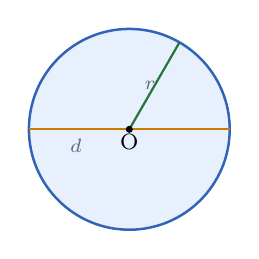
\begin{tikzpicture}[scale=0.85]
\fill[tmBlue!12] (0,0) circle (1.5); \draw[geo] (0,0) circle (1.5);
\draw[line width=0.8pt,tmOrange!80!black] (-1.5,0)--(1.5,0);
\draw[line width=0.8pt,tmGreen!70!black] (0,0)--(60:1.5);
\fill (0,0) circle (1.5pt); \node[lbl,below] at (0,0){O};
\node[dim,above left] at (40:0.7){$r$}; \node[dim,below] at (-0.8,0){$d$};
\end{tikzpicture}
\end{minipage}
\end{knowbox}
\gap
\begin{exbox}{\ExWord\ 1}
Tính chu vi và diện tích hình tròn có bán kính $5$ cm.
\guide
$C=5\times2\times3{,}14=31{,}4$ cm.\par $S=5\times5\times3{,}14=78{,}5$ cm$^2$.
\dapso{$31{,}4$ cm; $78{,}5$ cm$^2$.}
\end{exbox}
\gap
\begin{exbox}{\ExWord\ 2}
Một hình tròn có chu vi $18{,}84$ dm. Tính diện tích hình tròn đó.
\guide
Đường kính: $18{,}84:3{,}14=6$ dm; bán kính: $3$ dm.\par $S=3\times3\times3{,}14=28{,}26$ dm$^2$.
\dapso{$28{,}26$ dm$^2$.}
\end{exbox}
\gap
\begin{exbox}{\ExWord\ 3}
\begin{minipage}[t]{0.66\linewidth}
Một hình vuông có cạnh $10$ cm. Một hình tròn nằm trong hình vuông và tiếp xúc với cả bốn cạnh. Tính diện tích phần tô màu (phần hình vuông nằm ngoài hình tròn).
\end{minipage}\hfill
\begin{minipage}[t]{0.3\linewidth}\vspace{0pt}\centering
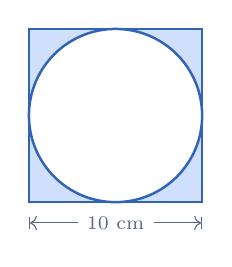
\begin{tikzpicture}[scale=0.22]
\fill[shade] (0,0) rectangle (10,10); \fill[white] (5,5) circle (5);
\draw[geo] (0,0) rectangle (10,10); \draw[geo] (5,5) circle (5);
\draw[|<->|,Slate] (0,-1.2)--node[fill=white,dim]{$10$ cm}(10,-1.2);
\end{tikzpicture}
\end{minipage}
\guide
Đường kính hình tròn bằng cạnh hình vuông: $d=10$ cm, $r=5$ cm.\par
$S_\text{hình vuông}=10\times10=100$ cm$^2$;\par $S_\text{hình tròn}=5\times5\times3{,}14=78{,}5$ cm$^2$.\par
Phần tô màu: $100-78{,}5=21{,}5$ cm$^2$.
\dapso{$21{,}5$ cm$^2$.}
\end{exbox}
\gap
\begin{exbox}{\ExWord\ 4}
Bánh xe của một chiếc xe kéo có đường kính $0{,}6$ m. Hỏi xe đi được bao nhiêu mét khi bánh xe lăn được $100$ vòng?
\guide
Mỗi vòng lăn, xe đi được quãng đường bằng chu vi bánh xe: $0{,}6\times3{,}14=1{,}884$ m.\par
$100$ vòng: $1{,}884\times100=188{,}4$ m.
\dapso{$188{,}4$ m.}
\end{exbox}
\dividerbar{Luyện tập}
\begin{probbox}{1}{\relax}
Tính chu vi và diện tích hình tròn có:
\begin{cols3}
\pa{a} $r=3$ cm; & \pa{b} $r=0{,}5$ dm; & \pa{c} $d=8$ m.
\end{cols3}
\end{probbox}
\probsol{
\pa{a} $C=18{,}84$ cm; $S=28{,}26$ cm$^2$.\par \pa{b} $C=3{,}14$ dm; $S=0{,}785$ dm$^2$.\par \pa{c} $C=25{,}12$ m; $r=4$ m, $S=50{,}24$ m$^2$.
\dapso{Xem ở trên.}}
\gap
\begin{probbox}{2}{\relax}
Một hình tròn có chu vi $12{,}56$ cm. Tính bán kính và diện tích hình tròn đó.
\end{probbox}
\probsol{
$d=12{,}56:3{,}14=4$ cm; $r=2$ cm.\par $S=2\times2\times3{,}14=12{,}56$ cm$^2$.
\dapso{$r=2$ cm; $S=12{,}56$ cm$^2$.}}
\gap
\begin{probbox}{3}{\relax}
Bánh xe đạp có đường kính $65$ cm. Hỏi xe đạp đi được bao nhiêu ki-lô-mét khi bánh xe lăn $1\,000$ vòng?
\end{probbox}
\probsol{
Mỗi vòng: $65\times3{,}14=204{,}1$ cm.\par $1\,000$ vòng: $204\,100$ cm $=2{,}041$ km.
\dapso{$2{,}041$ km.}}
\gap
\begin{probbox}{4}{\relax}
Bánh xe ô tô đi được $1\,099$ m khi lăn $500$ vòng. Tính đường kính bánh xe.
\end{probbox}
\probsol{
Chu vi: $1\,099:500=2{,}198$ m.\par Đường kính: $2{,}198:3{,}14=0{,}7$ m.
\dapso{$0{,}7$ m.}}
\gap
\begin{probbox}{5}{\relax}
Kim phút của một chiếc đồng hồ dài $10$ cm. Hỏi đầu kim phút đi được quãng đường bao nhiêu trong $1$ giờ? Trong $15$ phút?
\end{probbox}
\probsol{
Trong $1$ giờ, đầu kim đi hết một vòng: $10\times2\times3{,}14=62{,}8$ cm.\par Trong $15$ phút, đi một phần tư vòng: $62{,}8:4=15{,}7$ cm.
\dapso{$62{,}8$ cm; $15{,}7$ cm.}}
\gap
\begin{probbox}{6}{\relax}
Tính diện tích và chu vi của nửa hình tròn có đường kính $8$ cm.
\end{probbox}
\probsol{
$S=4\times4\times3{,}14:2=25{,}12$ cm$^2$.\par Chu vi bằng nửa chu vi hình tròn cộng với đường kính: $8\times3{,}14:2+8=20{,}56$ cm.
\dapso{$25{,}12$ cm$^2$; $20{,}56$ cm.}}
\gap
\begin{probbox}{7}{\relax}
Một bồn hoa hình tròn có bán kính $10$ m. Người ta làm một lối đi rộng $1$ m bao quanh bồn hoa. Tính diện tích lối đi.
\end{probbox}
\probsol{
Hình tròn bên ngoài có bán kính $11$ m.\par Lối đi: $11\times11\times3{,}14-10\times10\times3{,}14=(121-100)\times3{,}14=65{,}94$ m$^2$.
\dapso{$65{,}94$ m$^2$.}}
\gap
\begin{probbox}{8}{\relax}
Một hình vuông nằm trong hình tròn bán kính $5$ cm, bốn đỉnh của hình vuông nằm trên đường tròn. Tính diện tích phần hình tròn nằm ngoài hình vuông.
\end{probbox}
\probsol{
Hai đường chéo của hình vuông là đường kính, dài $10$ cm, và chia hình vuông thành $4$ tam giác vuông có cạnh góc vuông $5$ cm: $S_\text{hình vuông}=4\times5\times5:2=50$ cm$^2$.\par
$S_\text{hình tròn}=78{,}5$ cm$^2$.\par Phần cần tìm: $78{,}5-50=28{,}5$ cm$^2$.
\dapso{$28{,}5$ cm$^2$.}}
\gap
\begin{probbox}{9}{\relax}
Nếu bán kính hình tròn gấp lên $3$ lần thì chu vi và diện tích của nó gấp lên bao nhiêu lần? Thử lại với $r=1$ cm.
\end{probbox}
\probsol{
Chu vi gấp lên $3$ lần và diện tích gấp lên $3\times3=9$ lần.\par Ví dụ: $r=1$: $C=6{,}28$, $S=3{,}14$; $r=3$: $C=18{,}84=6{,}28\times3$, $S=28{,}26=3{,}14\times9$.
\dapso{$3$ lần; $9$ lần.}}
\gap
\begin{probbox}{10}{\relax}
Tính chu vi và diện tích hình tròn có bán kính $3$ cm.
\end{probbox}
\probsol{
$C=3\times2\times3{,}14=18{,}84$ cm.\par $S=3\times3\times3{,}14=28{,}26$ cm$^2$.
\dapso{$C=18{,}84$ cm; $S=28{,}26$ cm$^2$.}}
\gap
\begin{probbox}{11}{\relax}
Tính chu vi và diện tích hình tròn có bán kính $2{,}5$ cm.
\end{probbox}
\probsol{
$C=2{,}5\times2\times3{,}14=15{,}7$ cm.\par $S=2{,}5\times2{,}5\times3{,}14=19{,}625$ cm$^2$.
\dapso{$C=15{,}7$ cm; $S=19{,}625$ cm$^2$.}}
\gap
\begin{probbox}{12}{\relax}
Tính chu vi và diện tích hình tròn có bán kính $0{,}8$ m.
\end{probbox}
\probsol{
$C=0{,}8\times2\times3{,}14=5{,}024$ m.\par $S=0{,}8\times0{,}8\times3{,}14=2{,}0096$ m$^2$.
\dapso{$C=5{,}024$ m; $S=2{,}0096$ m$^2$.}}
\gap
\begin{probbox}{13}{\relax}
Tính chu vi và diện tích hình tròn có bán kính $12$ dm.
\end{probbox}
\probsol{
$C=12\times2\times3{,}14=75{,}36$ dm.\par $S=12\times12\times3{,}14=452{,}16$ dm$^2$.
\dapso{$C=75{,}36$ dm; $S=452{,}16$ dm$^2$.}}
\gap
\begin{probbox}{14}{\relax}
Tính chu vi và diện tích hình tròn có đường kính $10$ cm.
\end{probbox}
\probsol{
$C=10\times3{,}14=31{,}4$ cm.\par Bán kính: $10:2=5$ cm.\par $S=5\times5\times3{,}14=78{,}5$ cm$^2$.
\dapso{$C=31{,}4$ cm; $S=78{,}5$ cm$^2$.}}
\gap
\begin{probbox}{15}{\relax}
Tính chu vi và diện tích hình tròn có đường kính $4{,}2$ cm.
\end{probbox}
\probsol{
$C=4{,}2\times3{,}14=13{,}188$ cm.\par Bán kính: $4{,}2:2=2{,}1$ cm.\par $S=2{,}1\times2{,}1\times3{,}14=13{,}8474$ cm$^2$.
\dapso{$C=13{,}188$ cm; $S=13{,}8474$ cm$^2$.}}
\gap
\begin{probbox}{16}{\relax}
Tính chu vi và diện tích hình tròn có đường kính $2{,}4$ m.
\end{probbox}
\probsol{
$C=2{,}4\times3{,}14=7{,}536$ m.\par Bán kính: $2{,}4:2=1{,}2$ m.\par $S=1{,}2\times1{,}2\times3{,}14=4{,}5216$ m$^2$.
\dapso{$C=7{,}536$ m; $S=4{,}5216$ m$^2$.}}
\gap
\begin{probbox}{17}{\relax}
Một hình tròn có chu vi $43{,}96$ cm. Tính bán kính và diện tích hình tròn đó.
\end{probbox}
\probsol{
Đường kính: $43{,}96:3{,}14=14$ cm.\par Bán kính: $14:2=7$ cm.\par $S=7\times7\times3{,}14=153{,}86$ cm$^2$.
\dapso{$r=7$ cm; $S=153{,}86$ cm$^2$.}}
\gap
\begin{probbox}{18}{\relax}
Một hình tròn có chu vi $21{,}98$ cm. Tính bán kính và diện tích hình tròn đó.
\end{probbox}
\probsol{
Đường kính: $21{,}98:3{,}14=7$ cm.\par Bán kính: $7:2=3{,}5$ cm.\par $S=3{,}5\times3{,}5\times3{,}14=38{,}465$ cm$^2$.
\dapso{$r=3{,}5$ cm; $S=38{,}465$ cm$^2$.}}
\gap
\begin{probbox}{19}{\relax}
Một hình tròn có chu vi $6{,}28$ m. Tính bán kính và diện tích hình tròn đó.
\end{probbox}
\probsol{
Đường kính: $6{,}28:3{,}14=2$ m.\par Bán kính: $2:2=1$ m.\par $S=1\times1\times3{,}14=3{,}14$ m$^2$.
\dapso{$r=1$ m; $S=3{,}14$ m$^2$.}}
\gap
\begin{probbox}{20}{\relax}
Một hình tròn có diện tích $113{,}04$ cm$^2$. Tính bán kính và chu vi hình tròn đó.
\end{probbox}
\probsol{
$r\times r=113{,}04:3{,}14=36$.\par Vì $6\times6=36$ nên $r=6$ cm.\par $C=6\times2\times3{,}14=37{,}68$ cm.
\dapso{$r=6$ cm; $C=37{,}68$ cm.}}
\gap
\begin{probbox}{21}{\relax}
Một hình tròn có diện tích $12{,}56$ m$^2$. Tính bán kính và chu vi hình tròn đó.
\end{probbox}
\probsol{
$r\times r=12{,}56:3{,}14=4$.\par Vì $2\times2=4$ nên $r=2$ m.\par $C=2\times2\times3{,}14=12{,}56$ m.
\dapso{$r=2$ m; $C=12{,}56$ m.}}
\gap
\begin{probbox}{22}{\relax}
Một bánh xe có đường kính $0{,}5$ m. Hỏi bánh xe lăn $200$ vòng thì đi được bao nhiêu mét?
\end{probbox}
\probsol{
Một vòng: $0{,}5\times3{,}14=1{,}57$ m.\par $200$ vòng: $1{,}57\times200=314$ m.
\dapso{$314$ m.}}
\gap
\begin{probbox}{23}{\relax}
Một bánh xe có đường kính $0{,}7$ m. Hỏi bánh xe lăn $1\,000$ vòng thì đi được bao nhiêu mét?
\end{probbox}
\probsol{
Một vòng: $0{,}7\times3{,}14=2{,}198$ m.\par $1\,000$ vòng: $2{,}198\times1\,000=2\,198$ m.
\dapso{$2\,198$ m.}}
\gap
\begin{probbox}{24}{\relax}
Bánh xe đạp đi được $816{,}4$ m khi lăn $400$ vòng. Tính đường kính bánh xe.
\end{probbox}
\probsol{
Một vòng: $816{,}4:400=2{,}041$ m.\par Đường kính: $2{,}041:3{,}14=0{,}65$ m.
\dapso{$0{,}65$ m.}}
\gap
\begin{probbox}{25}{\relax}
Tính diện tích và chu vi của nửa hình tròn có đường kính $10$ cm.
\end{probbox}
\probsol{
Diện tích: $5\times5\times3{,}14:2=39{,}25$ cm$^2$.\par Nửa đường tròn: $10\times3{,}14:2=15{,}7$ cm.\par Chu vi (tính cả đường kính): $15{,}7+10=25{,}7$ cm.
\dapso{$S=39{,}25$ cm$^2$; chu vi $25{,}7$ cm.}}
\gap
\begin{probbox}{26}{\relax}
Tính diện tích và chu vi của nửa hình tròn có đường kính $6$ cm.
\end{probbox}
\probsol{
Diện tích: $3\times3\times3{,}14:2=14{,}13$ cm$^2$.\par Nửa đường tròn: $6\times3{,}14:2=9{,}42$ cm.\par Chu vi (tính cả đường kính): $9{,}42+6=15{,}42$ cm.
\dapso{$S=14{,}13$ cm$^2$; chu vi $15{,}42$ cm.}}
\gap
\begin{probbox}{27}{\relax}
Cánh quạt trần dài $0{,}6$ m tính từ tâm. Tính diện tích hình tròn mà đầu cánh quạt quét được.
\end{probbox}
\probsol{
Bán kính $r=0{,}6$ m.\par $S=0{,}6\times0{,}6\times3{,}14=1{,}1304$ m$^2$.
\dapso{$1{,}1304$ m$^2$.}}
\gap
\begin{probbox}{28}{\relax}
Một cái ao hình tròn có đường kính $20$ m. Tiền làm hàng rào là $50\,000$ đồng mỗi mét. Hỏi làm hàng rào quanh ao hết bao nhiêu tiền?
\end{probbox}
\probsol{
Chu vi: $20\times3{,}14=62{,}8$ m.\par Số tiền: $50\,000\times62{,}8=3\,140\,000$ đồng.
\dapso{$3\,140\,000$ đồng.}}
\gap
\begin{probbox}{29}{\relax}
Tính diện tích một phần tư hình tròn có bán kính $4$ cm.
\end{probbox}
\probsol{
Cả hình tròn: $4\times4\times3{,}14=50{,}24$ cm$^2$.\par Một phần tư: $50{,}24:4=12{,}56$ cm$^2$.
\dapso{$12{,}56$ cm$^2$.}}
\gap
\begin{probbox}{30}{\relax}
Tính diện tích một phần tư hình tròn có bán kính $10$ cm.
\end{probbox}
\probsol{
Cả hình tròn: $10\times10\times3{,}14=314$ cm$^2$.\par Một phần tư: $314:4=78{,}5$ cm$^2$.
\dapso{$78{,}5$ cm$^2$.}}
\dividerbar{Thử thách -- Nâng cao}
\begin{probbox}{31}{\stars{1}}
Một hình tròn có diện tích $50{,}24$ cm$^2$. Tính chu vi hình tròn đó.
\end{probbox}
\probsol{
$r\times r=50{,}24:3{,}14=16$, nên $r=4$ cm.\par $C=4\times2\times3{,}14=25{,}12$ cm.
\dapso{$25{,}12$ cm.}}
\gap
\begin{probbox}{32}{\stars{1}}
Nếu bán kính hình tròn tăng thêm $2$ cm thì chu vi tăng thêm bao nhiêu? Kết quả có phụ thuộc vào bán kính ban đầu không?
\end{probbox}
\probsol{
Phần tăng thêm là $(r+2)\times2\times3{,}14-r\times2\times3{,}14=2\times2\times3{,}14=12{,}56$ cm, dù bán kính ban đầu là bao nhiêu.
\dapso{$12{,}56$ cm; không phụ thuộc.}}
\gap
\begin{probbox}{33}{\stars{1}}
Một nửa hình tròn lớn có đường kính $AB=12$ cm. M là trung điểm của AB; vẽ hai nửa hình tròn nhỏ có đường kính AM và MB. So sánh độ dài nửa đường tròn lớn với tổng độ dài hai nửa đường tròn nhỏ.
\end{probbox}
\probsol{
Nửa đường tròn lớn: $12\times3{,}14:2=18{,}84$ cm.\par Mỗi nửa đường tròn nhỏ: $6\times3{,}14:2=9{,}42$ cm; cả hai: $18{,}84$ cm.\par Hai độ dài bằng nhau.
\dapso{Bằng nhau ($18{,}84$ cm).}}
\gap
\begin{probbox}{34}{\stars{1}}
Hai hình tròn có cùng tâm O, bán kính $3$ cm và $5$ cm. Tính diện tích phần nằm giữa hai đường tròn (hình vành khăn).
\end{probbox}
\probsol{
$S=5\times5\times3{,}14-3\times3\times3{,}14=(25-9)\times3{,}14=50{,}24$ cm$^2$.
\dapso{$50{,}24$ cm$^2$.}}
\gap
\begin{probbox}{35}{\stars{2}}
\begin{minipage}[t]{0.66\linewidth}
Hình vuông ABCD có cạnh $8$ cm. Vẽ bốn phần tư hình tròn bán kính $4$ cm có tâm là bốn đỉnh của hình vuông. Tính diện tích phần tô màu.
\end{minipage}\hfill
\begin{minipage}[t]{0.3\linewidth}\vspace{0pt}\centering
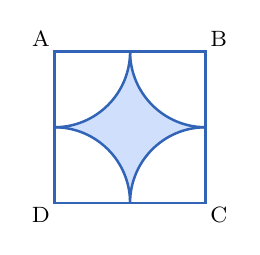
\begin{tikzpicture}[scale=0.24]
\fill[shade] (0,0) rectangle (8,8);
\foreach \x/\y/\a in {0/0/0,8/0/90,8/8/180,0/8/270}{\fill[white] (\x,\y) -- ++(\a:4) arc (\a:\a+90:4) -- cycle; \draw[geo] (\x,\y) ++(\a:4) arc (\a:\a+90:4);}
\draw[geo] (0,0) rectangle (8,8);
\node[lbl,below left] at (0,0){D}; \node[lbl,below right] at (8,0){C}; \node[lbl,above right] at (8,8){B}; \node[lbl,above left] at (0,8){A};
\end{tikzpicture}
\end{minipage}
\end{probbox}
\probsol{
Bốn phần tư hình tròn bán kính $4$ cm ghép lại thành một hình tròn: $4\times4\times3{,}14=50{,}24$ cm$^2$.\par
Phần tô màu: $8\times8-50{,}24=13{,}76$ cm$^2$.
\dapso{$13{,}76$ cm$^2$.}}
\gap
\begin{probbox}{36}{\stars{2}}
\begin{minipage}[t]{0.66\linewidth}
Hình vuông ABCD có cạnh $10$ cm. Vẽ hai phần tư hình tròn bán kính $10$ cm có tâm B và D; phần chung của chúng là ``chiếc lá'' được tô màu. Tính diện tích chiếc lá.
\end{minipage}\hfill
\begin{minipage}[t]{0.3\linewidth}\vspace{0pt}\centering
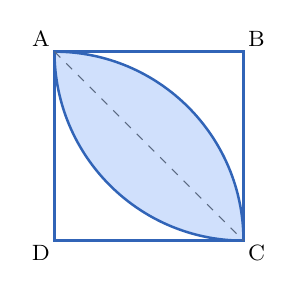
\begin{tikzpicture}[scale=0.24]
\fill[shade] (10,0) arc (0:90:10) arc (180:270:10);
\draw[geo] (0,0) rectangle (10,10);
\draw[geo] (10,0) arc (0:90:10); \draw[geo] (0,10) arc (180:270:10);
\draw[dashed,Slate] (0,10)--(10,0);
\node[lbl,below left] at (0,0){D}; \node[lbl,below right] at (10,0){C}; \node[lbl,above right] at (10,10){B}; \node[lbl,above left] at (0,10){A};
\end{tikzpicture}
\end{minipage}
\end{probbox}
\probsol{
Đường chéo AC chia chiếc lá thành hai nửa bằng nhau.\par Mỗi nửa bằng một phần tư hình tròn trừ đi một tam giác vuông:\par
$10\times10\times3{,}14:4-10\times10:2=78{,}5-50=28{,}5$ cm$^2$.\par
Chiếc lá: $28{,}5\times2=57$ cm$^2$.
\dapso{$57$ cm$^2$.}}
\gap
\begin{probbox}{37}{\stars{1}}
Hai hình tròn cùng tâm có bán kính $4$ m và $6$ m. Tính diện tích hình vành khăn nằm giữa hai đường tròn.
\end{probbox}
\probsol{
Hình tròn lớn: $6\times6\times3{,}14=113{,}04$ m$^2$.\par Hình tròn nhỏ: $4\times4\times3{,}14=50{,}24$ m$^2$.\par Diện tích cần tìm: $113{,}04-50{,}24=62{,}8$ m$^2$.
\dapso{$62{,}8$ m$^2$.}}
\gap
\begin{probbox}{38}{\stars{1}}
Một bồn hoa hình tròn có bán kính $8$ m, xung quanh có lối đi rộng $2$ m. Tính diện tích lối đi.
\end{probbox}
\probsol{
Hình tròn lớn: $10\times10\times3{,}14=314$ m$^2$.\par Hình tròn nhỏ: $8\times8\times3{,}14=200{,}96$ m$^2$.\par Diện tích cần tìm: $314-200{,}96=113{,}04$ m$^2$.
\dapso{$113{,}04$ m$^2$.}}
\gap
\begin{probbox}{39}{\stars{1}}
Một hình vuông có bốn đỉnh nằm trên đường tròn bán kính $6$ cm. Tính diện tích phần hình tròn nằm ngoài hình vuông.
\end{probbox}
\probsol{
Hai đường chéo của hình vuông là đường kính, dài $12$ cm và vuông góc với nhau.\par Hình vuông gồm $4$ tam giác vuông có cạnh góc vuông $6$ cm: $6\times6:2\times4=72$ cm$^2$.\par Hình tròn: $6\times6\times3{,}14=113{,}04$ cm$^2$.\par Phần cần tìm: $113{,}04-72=41{,}04$ cm$^2$.
\dapso{$41{,}04$ cm$^2$.}}
\gap
\begin{probbox}{40}{\stars{1}}
Một bánh xe nhỏ bán kính $0{,}3$ m lăn $150$ vòng. Một bánh xe lớn đi hết cùng quãng đường đó trong $90$ vòng. Tính bán kính bánh xe lớn.
\end{probbox}
\probsol{
Quãng đường: $0{,}3\times2\times3{,}14\times150=282{,}6$ m.\par Một vòng bánh lớn: $282{,}6:90=3{,}14$ m.\par Bán kính: $3{,}14:3{,}14:2=0{,}5$ m.
\dapso{$0{,}5$ m.}}
\gap
\begin{probbox}{41}{\stars{1}}
Một hình tròn có chu vi bằng chu vi hình vuông cạnh $15{,}7$ cm. Hình nào có diện tích lớn hơn và lớn hơn bao nhiêu?
\end{probbox}
\probsol{
Chu vi hình vuông: $62{,}8$ cm.\par Bán kính hình tròn: $62{,}8:3{,}14:2=10$ cm; diện tích $314$ cm$^2$.\par Diện tích hình vuông: $15{,}7\times15{,}7=246{,}49$ cm$^2$.\par Hình tròn lớn hơn $67{,}51$ cm$^2$.
\dapso{Hình tròn, lớn hơn $67{,}51$ cm$^2$.}}
\gap
\begin{probbox}{42}{\stars{1}}
Một hình tròn có diện tích $12{,}56$ cm$^2$. Nếu bán kính gấp đôi thì diện tích mới là bao nhiêu?
\end{probbox}
\probsol{
Gấp đôi $r$ thì $r\times r$ gấp lên $2\times2=4$ lần.\par Diện tích mới: $12{,}56\times4=50{,}24$ cm$^2$.
\dapso{$50{,}24$ cm$^2$.}}
\gap
\begin{probbox}{43}{\stars{1}}
Bán kính một hình tròn tăng thêm $1{,}5$ cm. Hỏi chu vi tăng thêm bao nhiêu?
\end{probbox}
\probsol{
$C=r\times2\times3{,}14$, nên $C$ tăng thêm $1{,}5\times2\times3{,}14=9{,}42$ cm.\par Kết quả này không phụ thuộc vào bán kính ban đầu.
\dapso{$9{,}42$ cm.}}
\gap
\begin{probbox}{44}{\stars{1}}
Một chiếc xe đạp cổ có bánh trước đường kính $0{,}5$ m và bánh sau đường kính $1$ m. Khi bánh sau lăn $100$ vòng thì bánh trước lăn bao nhiêu vòng?
\end{probbox}
\probsol{
Quãng đường: $1\times3{,}14\times100=314$ m.\par Một vòng bánh trước: $0{,}5\times3{,}14=1{,}57$ m.\par Số vòng bánh trước: $314:1{,}57=200$.
\dapso{$200$ vòng.}}
\gap
\begin{probbox}{45}{\stars{1}}
Một đường chạy gồm hai đoạn thẳng dài $100$ m và hai đầu là nửa hình tròn đường kính $60$ m. Tính độ dài một vòng chạy và diện tích phần bên trong.
\end{probbox}
\probsol{
Hai nửa hình tròn ghép thành một hình tròn: $60\times3{,}14=188{,}4$ m.\par Một vòng chạy: $100\times2+188{,}4=388{,}4$ m.\par Hình chữ nhật: $6\,000$ m$^2$; hình tròn: $30\times30\times3{,}14=2\,826$ m$^2$.\par Diện tích bên trong: $8\,826$ m$^2$.
\dapso{$388{,}4$ m; $8\,826$ m$^2$.}}
\gap
\begin{probbox}{46}{\stars{2}}
Từ một tấm bìa hình tròn bán kính $10$ cm, người ta cắt đi một phần tư hình tròn (giới hạn bởi hai bán kính vuông góc). Tính diện tích và chu vi phần còn lại.
\end{probbox}
\probsol{
Hình tròn: $314$ cm$^2$; ba phần tư: $235{,}5$ cm$^2$.\par Chu vi hình tròn $62{,}8$ cm; phần cung còn lại: $47{,}1$ cm.\par Chu vi: cung cộng hai bán kính, $47{,}1+20=67{,}1$ cm.
\dapso{$235{,}5$ cm$^2$; $67{,}1$ cm.}}
\gap
\begin{probbox}{47}{\stars{2}}
Một con dê được buộc vào một góc bên ngoài của chuồng hình vuông cạnh $6$ m bằng sợi dây dài $4$ m. Dê không vào được trong chuồng. Tính diện tích phần cỏ mà dê có thể ăn được.
\end{probbox}
\probsol{
Sợi dây ngắn hơn cạnh chuồng nên dê chỉ đi vòng quanh góc đó.\par Chuồng che mất $\dfrac14$ hình tròn, còn lại $\dfrac34$ hình tròn bán kính $4$ m.\par Diện tích: $4\times4\times3{,}14\times\dfrac34=37{,}68$ m$^2$.
\dapso{$37{,}68$ m$^2$.}}
\gap
\begin{probbox}{48}{\stars{1}}
Chu vi của hai hình tròn hơn kém nhau $12{,}56$ cm, bán kính hình lớn gấp $3$ lần bán kính hình bé. Tính diện tích hình tròn lớn.
\end{probbox}
\probsol{
Hiệu hai bán kính: $12{,}56:2:3{,}14=2$ cm.\par $3-1=2$ phần ứng với $2$ cm, nên hai bán kính là $1$ cm và $3$ cm.\par Diện tích hình tròn lớn: $3\times3\times3{,}14=28{,}26$ cm$^2$.
\dapso{$28{,}26$ cm$^2$.}}
\gap
\begin{probbox}{49}{\stars{1}}
Kim phút dài $12$ cm. Hỏi trong $20$ phút kim phút quét được diện tích bao nhiêu?
\end{probbox}
\probsol{
$20$ phút là $\dfrac13$ vòng.\par Hình tròn: $12\times12\times3{,}14=452{,}16$ cm$^2$.\par Diện tích quét được: $452{,}16:3=150{,}72$ cm$^2$.
\dapso{$150{,}72$ cm$^2$.}}
\gap
\begin{probbox}{50}{\stars{1}}
Bánh xe máy cày có đường kính $0{,}7$ m, mỗi phút lăn được $120$ vòng. Hỏi trong $10$ phút máy cày đi được bao nhiêu mét?
\end{probbox}
\probsol{
Một vòng: $0{,}7\times3{,}14=2{,}198$ m.\par Số vòng trong $10$ phút: $1\,200$.\par Quãng đường: $2{,}198\times1\,200=2\,637{,}6$ m.
\dapso{$2\,637{,}6$ m.}}
\clearpage
\titlehead
\begingroup\setbox0=\vbox{\section*{Luyện tập tính diện tích}}\endgroup
\chapterhead{15}{Luyện tập tính diện tích}

\shead{Chia nhỏ, ghép thêm, cắt bớt}
\begin{knowbox}
Để tính diện tích một hình ghép, ta đưa về các hình đã biết công thức tính diện tích:
\begin{center}\renewcommand{\arraystretch}{1.5}
\begin{tabular}{|l|c||l|c|}\hline
Hình chữ nhật & $a\times b$ & Hình tam giác & $a\times h:2$\\\hline
Hình vuông & $a\times a$ & Hình thang & $(a+b)\times h:2$\\\hline
Hình tròn & $r\times r\times3{,}14$ & Nửa hình tròn & $r\times r\times3{,}14:2$\\\hline
\end{tabular}\end{center}
\begin{itemize}[leftmargin=1.4em,itemsep=3pt]
\item \textbf{Chia nhỏ:} chia hình thành các phần quen thuộc rồi \emph{cộng} diện tích các phần.
\item \textbf{Ghép thêm rồi trừ đi:} bổ sung thành một hình lớn quen thuộc rồi \emph{trừ} đi phần đã ghép thêm.
\item Luôn đổi các số đo về \textbf{cùng một đơn vị} trước; $1$ m$^2=100$ dm$^2=10\,000$ cm$^2$.
\end{itemize}
\end{knowbox}
\gap
\begin{exbox}{\ExWord\ 1}
\begin{minipage}[t]{0.62\linewidth}
Một mảnh đất có hình dạng như hình vẽ: một hình chữ nhật có chiều dài $20$ m, chiều rộng $12$ m, phía trên là một hình tam giác có đáy bằng chiều dài hình chữ nhật và chiều cao $8$ m. Tính diện tích mảnh đất.
\end{minipage}\hfill
\begin{minipage}[t]{0.34\linewidth}\vspace{0pt}\centering
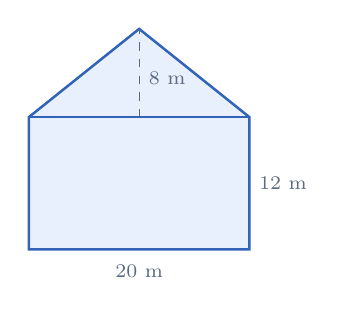
\begin{tikzpicture}[scale=0.14]
\fill[tmBlue!12] (0,0)--(20,0)--(20,12)--(10,20)--(0,12)--cycle;
\draw[geo] (0,0)--(20,0)--(20,12)--(10,20)--(0,12)--cycle; \draw[geo] (0,12)--(20,12);
\draw[dashed,Slate] (10,12)--(10,20);
\node[dim] at (10,-2){$20$ m}; \node[dim,right] at (20,6){$12$ m}; \node[dim,right] at (10,15.5){$8$ m};
\end{tikzpicture}
\end{minipage}
\guide
\textbf{Chia} mảnh đất thành một hình chữ nhật và một hình tam giác:\par
$S_\text{hình chữ nhật}=20\times12=240$ m$^2$;\par $S_\text{hình tam giác}=20\times8:2=80$ m$^2$.\par Mảnh đất: $240+80=320$ m$^2$.
\dapso{$320$ m$^2$.}
\end{exbox}
\gap
\begin{exbox}{\ExWord\ 2}
\begin{minipage}[t]{0.62\linewidth}
Từ một tấm gỗ hình chữ nhật có chiều dài $16$ cm, chiều rộng $10$ cm, người ta cắt đi một nửa hình tròn có đường kính bằng chiều rộng tấm gỗ (xem hình vẽ). Tính diện tích phần gỗ còn lại.
\end{minipage}\hfill
\begin{minipage}[t]{0.34\linewidth}\vspace{0pt}\centering
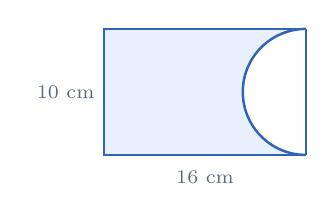
\begin{tikzpicture}[scale=0.16]
\fill[tmBlue!12] (0,0)--(16,0)--(16,10)--(0,10)--cycle; \fill[white] (16,0) arc (-90:-270:5);
\draw[geo] (16,0)--(0,0)--(0,10)--(16,10); \draw[geo] (16,10)--(16,0); \draw[geo] (16,0) arc (-90:-270:5);
\node[dim] at (8,-1.8){$16$ cm}; \node[dim,left] at (0,5){$10$ cm};
\end{tikzpicture}
\end{minipage}
\guide
$S_\text{tấm gỗ}=16\times10=160$ cm$^2$.\par Nửa hình tròn có $r=5$ cm: $5\times5\times3{,}14:2=39{,}25$ cm$^2$.\par
Phần gỗ còn lại: $160-39{,}25=120{,}75$ cm$^2$.
\dapso{$120{,}75$ cm$^2$.}
\end{exbox}
\gap
\begin{exbox}{\ExWord\ 3}
Trên bản đồ tỉ lệ $1:1\,000$, một khu vườn hình thang có hai đáy $5$ cm và $3$ cm, chiều cao $4$ cm. Tính diện tích thật của khu vườn.
\guide
Độ dài thật: $5$ cm $\to5\,000$ cm $=50$ m;\par $3$ cm $\to30$ m;\par $4$ cm $\to40$ m.\par
Diện tích thật: $(50+30)\times40:2=1\,600$ m$^2$.\par
\emph{Lưu ý:} đổi ra độ dài thật \emph{trước}, rồi mới tính diện tích.
\dapso{$1\,600$ m$^2$.}
\end{exbox}
\gap
\begin{exbox}{\ExWord\ 4}
Một nền nhà hình chữ nhật có chiều dài $8$ m, chiều rộng $6$ m. Người ta lát nền bằng loại gạch hình vuông cạnh $40$ cm, giá $25\,000$ đồng một viên. Cần bao nhiêu viên gạch và hết bao nhiêu tiền? (Không tính phần mạch vữa.)
\guide
Nền nhà: $8\times6=48$ m$^2$ $=480\,000$ cm$^2$.\par Một viên gạch: $40\times40=1\,600$ cm$^2$.\par
Số viên gạch: $480\,000:1\,600=300$.\par Số tiền: $25\,000\times300=7\,500\,000$ đồng.
\dapso{$300$ viên gạch; $7\,500\,000$ đồng.}
\end{exbox}
\dividerbar{Luyện tập}
\begin{probbox}{1}{\relax}
\begin{minipage}[t]{0.66\linewidth}
Tính diện tích hình chữ L (số đo tính bằng xăng-ti-mét).
\end{minipage}\hfill
\begin{minipage}[t]{0.3\linewidth}\vspace{0pt}\centering
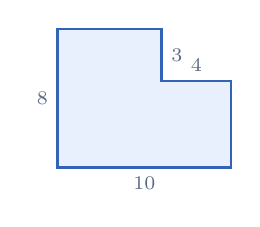
\begin{tikzpicture}[scale=0.22]
\fill[tmBlue!12] (0,0)--(10,0)--(10,5)--(6,5)--(6,8)--(0,8)--cycle;
\draw[geo] (0,0)--(10,0)--(10,5)--(6,5)--(6,8)--(0,8)--cycle;
\node[dim,below] at (5,0){$10$}; \node[dim,left] at (0,4){$8$}; \node[dim,above] at (8,5){$4$}; \node[dim,right] at (6,6.5){$3$};
\end{tikzpicture}
\end{minipage}
\end{probbox}
\probsol{
\emph{Ghép thêm rồi trừ đi:} $10\times8-4\times3=80-12=68$ cm$^2$.
\dapso{$68$ cm$^2$.}}
\gap
\begin{probbox}{2}{\relax}
Một mảnh đất hình chữ nhật có chiều dài $25$ m, chiều rộng bằng $\dfrac35$ chiều dài. Trên mảnh đất người ta xây một ngôi nhà có nền hình vuông cạnh $10$ m. Tính diện tích đất còn lại.
\end{probbox}
\probsol{
Chiều rộng: $25\times\dfrac35=15$ m.\par Còn lại: $25\times15-10\times10=375-100=275$ m$^2$.
\dapso{$275$ m$^2$.}}
\gap
\begin{probbox}{3}{\relax}
Một sân trường hình chữ nhật có chiều dài $50$ m, chiều rộng $30$ m. Ở giữa sân có một bồn hoa hình tròn bán kính $3$ m. Tính diện tích phần sân còn lại.
\end{probbox}
\probsol{
$50\times30-3\times3\times3{,}14=1\,500-28{,}26=1\,471{,}74$ m$^2$.
\dapso{$1\,471{,}74$ m$^2$.}}
\gap
\begin{probbox}{4}{\relax}
Một mảnh vườn hình thang có hai đáy $30$ m và $20$ m, chiều cao $16$ m. Người ta đào một phần tư diện tích để làm ao, phần còn lại để trồng cây. Tính diện tích trồng cây.
\end{probbox}
\probsol{
$S=(30+20)\times16:2=400$ m$^2$.\par Diện tích trồng cây: $400\times\dfrac34=300$ m$^2$.
\dapso{$300$ m$^2$.}}
\gap
\begin{probbox}{5}{\relax}
Trên bản đồ tỉ lệ $1:500$, một sân bóng hình chữ nhật có kích thước $6$ cm và $4$ cm. Tính diện tích thật của sân.
\end{probbox}
\probsol{
Kích thước thật: $6\times500=3\,000$ cm $=30$ m;\par $4\times500=2\,000$ cm $=20$ m.\par Diện tích: $30\times20=600$ m$^2$.
\dapso{$600$ m$^2$.}}
\gap
\begin{probbox}{6}{\relax}
Một phòng học có chiều dài $6$ m, chiều rộng $4$ m được lát bằng gạch hình vuông cạnh $50$ cm. Cần bao nhiêu viên gạch?
\end{probbox}
\probsol{
Phòng học: $24$ m$^2$ $=240\,000$ cm$^2$; một viên gạch: $2\,500$ cm$^2$.\par Số viên gạch: $240\,000:2\,500=96$.
\dapso{$96$ viên gạch.}}
\gap
\begin{probbox}{7}{\relax}
Người ta cắt bốn hình vuông bằng nhau cạnh $0{,}2$ m ở bốn góc của một tấm tôn hình chữ nhật có chiều dài $2$ m, chiều rộng $1{,}5$ m. Tính diện tích phần tôn còn lại.
\end{probbox}
\probsol{
$2\times1{,}5-4\times0{,}2\times0{,}2=3-0{,}16=2{,}84$ m$^2$.
\dapso{$2{,}84$ m$^2$.}}
\gap
\begin{probbox}{8}{\relax}
Một hình gồm một hình vuông cạnh $6$ cm và một nửa hình tròn vẽ ra phía ngoài trên một cạnh của hình vuông. Tính diện tích và chu vi của hình đó.
\end{probbox}
\probsol{
Diện tích: $6\times6+3\times3\times3{,}14:2=36+14{,}13=50{,}13$ cm$^2$.\par
Chu vi gồm ba cạnh hình vuông và nửa đường tròn: $6\times3+6\times3{,}14:2=18+9{,}42=27{,}42$ cm.
\dapso{$50{,}13$ cm$^2$; $27{,}42$ cm.}}
\gap
\begin{probbox}{9}{\relax}
Hai đường chéo của hình chữ nhật ABCD ($AB=12$ cm, $BC=8$ cm) cắt nhau tại O. Chứng tỏ rằng các hình tam giác OAB, OBC, OCD và ODA có diện tích bằng nhau, rồi tính diện tích mỗi hình.
\end{probbox}
\probsol{
O là trung điểm của mỗi đường chéo.\par Trong hình tam giác ABC, BO nối B với trung điểm của AC nên $S_{OAB}=S_{OBC}$; tương tự $S_{OBC}=S_{OCD}$ và $S_{OCD}=S_{ODA}$.\par
Mỗi hình tam giác: $12\times8:4=24$ cm$^2$.
\dapso{$24$ cm$^2$.}}
\gap
\begin{probbox}{10}{\relax}
Trên bản đồ tỉ lệ $1:1\,000$, một mảnh đất hình chữ nhật có kích thước $6$ cm và $4$ cm. Tính diện tích thật của mảnh đất.
\end{probbox}
\probsol{
Chiều dài thật: $6\times1\,000=6\,000$ cm $=60$ m.\par Chiều rộng thật: $4\times1\,000=4\,000$ cm $=40$ m.\par Diện tích: $60\times40=2\,400$ m$^2$.
\dapso{$2\,400$ m$^2$.}}
\gap
\begin{probbox}{11}{\relax}
Trên bản đồ tỉ lệ $1:2\,000$, một mảnh đất hình chữ nhật có kích thước $5$ cm và $3$ cm. Tính diện tích thật của mảnh đất.
\end{probbox}
\probsol{
Chiều dài thật: $5\times2\,000=10\,000$ cm $=100$ m.\par Chiều rộng thật: $3\times2\,000=6\,000$ cm $=60$ m.\par Diện tích: $100\times60=6\,000$ m$^2$.
\dapso{$6\,000$ m$^2$.}}
\gap
\begin{probbox}{12}{\relax}
Trên bản đồ tỉ lệ $1:500$, một mảnh đất hình chữ nhật có kích thước $8$ cm và $5$ cm. Tính diện tích thật của mảnh đất.
\end{probbox}
\probsol{
Chiều dài thật: $8\times500=4\,000$ cm $=40$ m.\par Chiều rộng thật: $5\times500=2\,500$ cm $=25$ m.\par Diện tích: $40\times25=1\,000$ m$^2$.
\dapso{$1\,000$ m$^2$.}}
\gap
\begin{probbox}{13}{\relax}
Nền một căn phòng có chiều dài $6$ m, chiều rộng $4$ m, được lát bằng gạch hình vuông cạnh $40$ cm, giá $20\,000$ đồng một viên. Tính số viên gạch và số tiền mua gạch (không tính mạch vữa).
\end{probbox}
\probsol{
Nền phòng: $6\times4=24$ m$^2$.\par Một viên gạch: $40\times40=1600$ cm$^2$ $=0{,}16$ m$^2$.\par Số viên gạch: $24:0{,}16=150$.\par Số tiền: $20\,000\times150=3\,000\,000$ đồng.
\dapso{$150$ viên gạch; $3\,000\,000$ đồng.}}
\gap
\begin{probbox}{14}{\relax}
Nền một căn phòng có chiều dài $8$ m, chiều rộng $5$ m, được lát bằng gạch hình vuông cạnh $50$ cm, giá $35\,000$ đồng một viên. Tính số viên gạch và số tiền mua gạch (không tính mạch vữa).
\end{probbox}
\probsol{
Nền phòng: $8\times5=40$ m$^2$.\par Một viên gạch: $50\times50=2500$ cm$^2$ $=0{,}25$ m$^2$.\par Số viên gạch: $40:0{,}25=160$.\par Số tiền: $35\,000\times160=5\,600\,000$ đồng.
\dapso{$160$ viên gạch; $5\,600\,000$ đồng.}}
\gap
\begin{probbox}{15}{\relax}
Nền một căn phòng có chiều dài $4{,}8$ m, chiều rộng $3{,}6$ m, được lát bằng gạch hình vuông cạnh $60$ cm, giá $45\,000$ đồng một viên. Tính số viên gạch và số tiền mua gạch (không tính mạch vữa).
\end{probbox}
\probsol{
Nền phòng: $4{,}8\times3{,}6=17{,}28$ m$^2$.\par Một viên gạch: $60\times60=3600$ cm$^2$ $=0{,}36$ m$^2$.\par Số viên gạch: $17{,}28:0{,}36=48$.\par Số tiền: $45\,000\times48=2\,160\,000$ đồng.
\dapso{$48$ viên gạch; $2\,160\,000$ đồng.}}
\gap
\begin{probbox}{16}{\relax}
Một mảnh đất hình chữ nhật có chiều dài $30$ m, chiều rộng bằng $\dfrac{2}{3}$ chiều dài. Trên đó người ta xây một ngôi nhà $12$ m $\times$ $8$ m. Tính diện tích đất còn lại.
\end{probbox}
\probsol{
Chiều rộng: $30\times\dfrac{2}{3}=20$ m.\par Mảnh đất: $600$ m$^2$.\par Ngôi nhà: $96$ m$^2$.\par Còn lại: $504$ m$^2$.
\dapso{$504$ m$^2$.}}
\gap
\begin{probbox}{17}{\relax}
Một mảnh đất hình chữ nhật có chiều dài $40$ m, chiều rộng bằng $\dfrac{3}{4}$ chiều dài. Trên đó người ta xây một ngôi nhà $15$ m $\times$ $10$ m. Tính diện tích đất còn lại.
\end{probbox}
\probsol{
Chiều rộng: $40\times\dfrac{3}{4}=30$ m.\par Mảnh đất: $1\,200$ m$^2$.\par Ngôi nhà: $150$ m$^2$.\par Còn lại: $1\,050$ m$^2$.
\dapso{$1\,050$ m$^2$.}}
\gap
\begin{probbox}{18}{\relax}
Một sân chơi hình chữ nhật có chiều dài $40$ m, chiều rộng $25$ m; ở giữa có một hố cát hình tròn bán kính $3$ m. Tính diện tích phần còn lại.
\end{probbox}
\probsol{
Sân chơi: $1000$ m$^2$.\par Hố cát: $3\times3\times3{,}14=28{,}26$ m$^2$.\par Phần còn lại: $971{,}74$ m$^2$.
\dapso{$971{,}74$ m$^2$.}}
\gap
\begin{probbox}{19}{\relax}
Một sân chơi hình chữ nhật có chiều dài $30$ m, chiều rộng $20$ m; ở giữa có một hố cát hình tròn bán kính $5$ m. Tính diện tích phần còn lại.
\end{probbox}
\probsol{
Sân chơi: $600$ m$^2$.\par Hố cát: $5\times5\times3{,}14=78{,}5$ m$^2$.\par Phần còn lại: $521{,}5$ m$^2$.
\dapso{$521{,}5$ m$^2$.}}
\gap
\begin{probbox}{20}{\relax}
Một hình gồm hình vuông cạnh $8$ cm và một nửa hình tròn vẽ ra phía ngoài trên một cạnh (đường kính $=$ cạnh đó). Tính diện tích của hình.
\end{probbox}
\probsol{
Hình vuông: $64$ cm$^2$.\par Nửa hình tròn bán kính $4$ cm: $25{,}12$ cm$^2$.\par Tổng: $89{,}12$ cm$^2$.
\dapso{$89{,}12$ cm$^2$.}}
\gap
\begin{probbox}{21}{\relax}
Một hình gồm hình vuông cạnh $10$ cm và một nửa hình tròn vẽ ra phía ngoài trên một cạnh (đường kính $=$ cạnh đó). Tính diện tích của hình.
\end{probbox}
\probsol{
Hình vuông: $100$ cm$^2$.\par Nửa hình tròn bán kính $5$ cm: $39{,}25$ cm$^2$.\par Tổng: $139{,}25$ cm$^2$.
\dapso{$139{,}25$ cm$^2$.}}
\gap
\begin{probbox}{22}{\relax}
Từ một tấm bìa $3$ dm $\times$ $2$ dm, người ta cắt ở mỗi góc một hình vuông cạnh $0{,}4$ dm. Tính diện tích phần bìa còn lại.
\end{probbox}
\probsol{
Tấm bìa: $6$ dm$^2$.\par Bốn hình vuông: $0{,}64$ dm$^2$.\par Còn lại: $5{,}36$ dm$^2$.
\dapso{$5{,}36$ dm$^2$.}}
\gap
\begin{probbox}{23}{\relax}
Từ một tấm bìa $5$ dm $\times$ $4$ dm, người ta cắt ở mỗi góc một hình vuông cạnh $0{,}5$ dm. Tính diện tích phần bìa còn lại.
\end{probbox}
\probsol{
Tấm bìa: $20$ dm$^2$.\par Bốn hình vuông: $1$ dm$^2$.\par Còn lại: $19$ dm$^2$.
\dapso{$19$ dm$^2$.}}
\gap
\begin{probbox}{24}{\relax}
Một mảnh vườn hình thang có hai đáy $40$ m và $30$ m, chiều cao $20$ m. $\dfrac{1}{5}$ diện tích vườn là ao; phần còn lại trồng rau, cứ $3$ kg trên mỗi m$^2$. Tính số rau thu hoạch được.
\end{probbox}
\probsol{
Mảnh vườn: $700$ m$^2$.\par Ao: $140$ m$^2$.\par Trồng rau: $560$ m$^2$.\par Thu hoạch: $560\times3=1\,680$ kg.
\dapso{$1\,680$ kg.}}
\gap
\begin{probbox}{25}{\relax}
Một mảnh vườn hình thang có hai đáy $60$ m và $40$ m, chiều cao $30$ m. $\dfrac{1}{3}$ diện tích vườn là ao; phần còn lại trồng rau, cứ $2$ kg trên mỗi m$^2$. Tính số rau thu hoạch được.
\end{probbox}
\probsol{
Mảnh vườn: $1\,500$ m$^2$.\par Ao: $500$ m$^2$.\par Trồng rau: $1\,000$ m$^2$.\par Thu hoạch: $1\,000\times2=2\,000$ kg.
\dapso{$2\,000$ kg.}}
\gap
\begin{probbox}{26}{\relax}
Một mảnh đất hình chữ L là hình chữ nhật $20$ m $\times$ $15$ m bị cắt bớt một góc hình chữ nhật $8$ m $\times$ $6$ m. Tính diện tích mảnh đất.
\end{probbox}
\probsol{
Hình chữ nhật lớn: $300$ m$^2$.\par Phần cắt bớt: $48$ m$^2$.\par Diện tích: $252$ m$^2$.
\dapso{$252$ m$^2$.}}
\gap
\begin{probbox}{27}{\relax}
Một mảnh đất hình chữ L là hình chữ nhật $30$ m $\times$ $24$ m bị cắt bớt một góc hình chữ nhật $12$ m $\times$ $10$ m. Tính diện tích mảnh đất.
\end{probbox}
\probsol{
Hình chữ nhật lớn: $720$ m$^2$.\par Phần cắt bớt: $120$ m$^2$.\par Diện tích: $600$ m$^2$.
\dapso{$600$ m$^2$.}}
\gap
\begin{probbox}{28}{\relax}
Một mảnh vườn hình chữ nhật có chu vi $60$ m, chiều rộng bằng $\dfrac{2}{3}$ chiều dài. Tính diện tích mảnh vườn.
\end{probbox}
\probsol{
Nửa chu vi: $30$ m.\par Tổng số phần: $5$; một phần: $6$ m.\par Chiều dài $18$ m, chiều rộng $12$ m.\par Diện tích: $216$ m$^2$.
\dapso{$216$ m$^2$.}}
\gap
\begin{probbox}{29}{\relax}
Một mảnh vườn hình chữ nhật có chu vi $84$ m, chiều rộng bằng $\dfrac{3}{4}$ chiều dài. Tính diện tích mảnh vườn.
\end{probbox}
\probsol{
Nửa chu vi: $42$ m.\par Tổng số phần: $7$; một phần: $6$ m.\par Chiều dài $24$ m, chiều rộng $18$ m.\par Diện tích: $432$ m$^2$.
\dapso{$432$ m$^2$.}}
\gap
\begin{probbox}{30}{\relax}
Một mảnh vườn hình chữ nhật có chu vi $100$ m, chiều rộng bằng $\dfrac{1}{4}$ chiều dài. Tính diện tích mảnh vườn.
\end{probbox}
\probsol{
Nửa chu vi: $50$ m.\par Tổng số phần: $5$; một phần: $10$ m.\par Chiều dài $40$ m, chiều rộng $10$ m.\par Diện tích: $400$ m$^2$.
\dapso{$400$ m$^2$.}}
\dividerbar{Thử thách -- Nâng cao}
\begin{probbox}{31}{\stars{1}}
Một mảnh vườn hình chữ nhật có chu vi $56$ m. Nếu tăng chiều rộng thêm $4$ m và giảm chiều dài đi $4$ m thì mảnh vườn trở thành hình vuông. Tính diện tích mảnh vườn.
\end{probbox}
\probsol{
Chiều dài hơn chiều rộng $4+4=8$ m; nửa chu vi là $28$ m.\par Chiều dài: $(28+8):2=18$ m; chiều rộng: $10$ m.\par Diện tích: $180$ m$^2$.
\dapso{$180$ m$^2$.}}
\gap
\begin{probbox}{32}{\stars{1}}
Nếu tăng chiều dài của một mảnh vườn hình chữ nhật thêm $5$ m thì diện tích tăng thêm $60$ m$^2$; nếu giảm chiều rộng đi $3$ m thì diện tích giảm đi $75$ m$^2$. Tính diện tích mảnh vườn.
\end{probbox}
\probsol{
Phần tăng thêm là hình chữ nhật có một cạnh $5$ m, cạnh kia bằng chiều rộng, nên chiều rộng là $60:5=12$ m.\par Phần giảm đi là hình chữ nhật có một cạnh $3$ m, cạnh kia bằng chiều dài, nên chiều dài là $75:3=25$ m.\par
Diện tích: $25\times12=300$ m$^2$.
\dapso{$300$ m$^2$.}}
\gap
\begin{probbox}{33}{\stars{1}}
\begin{minipage}[t]{0.62\linewidth}
Một vườn rau hình chữ nhật có chiều dài $40$ m, chiều rộng $25$ m, có hai lối đi rộng $2$ m vuông góc với nhau, chạy suốt chiều dài và chiều rộng của vườn (xem hình vẽ). Tính diện tích trồng rau.
\end{minipage}\hfill
\begin{minipage}[t]{0.34\linewidth}\vspace{0pt}\centering
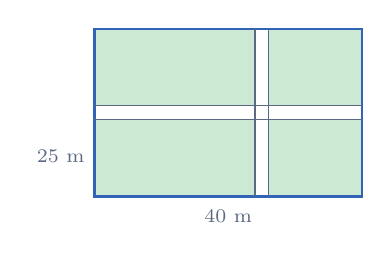
\begin{tikzpicture}[scale=0.085]
\fill[tmGreen!25] (0,0) rectangle (40,25);
\fill[white] (0,11.5) rectangle (40,13.5); \fill[white] (24,0) rectangle (26,25);
\draw[geo] (0,0) rectangle (40,25);
\draw[Slate] (0,11.5)--(40,11.5) (0,13.5)--(40,13.5) (24,0)--(24,25) (26,0)--(26,25);
\node[dim] at (20,-3){$40$ m}; \node[dim,left] at (0,6){$25$ m};
\end{tikzpicture}
\end{minipage}
\end{probbox}
\probsol{
Ghép các phần trồng rau lại với nhau, ta được hình chữ nhật có chiều dài $40-2=38$ m và chiều rộng $25-2=23$ m.\par
Diện tích trồng rau: $38\times23=874$ m$^2$.
\dapso{$874$ m$^2$.}}
\gap
\begin{probbox}{34}{\stars{1}}
Từ một tấm bìa hình chữ nhật có chiều dài $20$ cm, chiều rộng $10$ cm, người ta cắt ra hai hình tròn lớn nhất có thể, không chồng lên nhau. Tính diện tích phần bìa còn thừa.
\end{probbox}
\probsol{
Mỗi hình tròn có đường kính $10$ cm ($r=5$ cm), và hai hình tròn đặt cạnh nhau vừa đúng theo chiều dài $20$ cm.\par
Phần còn thừa: $20\times10-2\times5\times5\times3{,}14=200-157=43$ cm$^2$.
\dapso{$43$ cm$^2$.}}
\gap
\begin{probbox}{35}{\stars{2}}
Hình tam giác ABC vuông tại A có $AB=12$ cm, $AC=16$ cm và $BC=20$ cm. Vẽ ra phía ngoài các nửa hình tròn trên các cạnh AB, AC và BC. Chứng tỏ rằng nửa hình tròn trên BC có diện tích bằng tổng diện tích hai nửa hình tròn kia.
\end{probbox}
\probsol{
Nửa hình tròn trên AB ($r=6$): $6\times6\times3{,}14:2=56{,}52$ cm$^2$.\par
Nửa hình tròn trên AC ($r=8$): $8\times8\times3{,}14:2=100{,}48$ cm$^2$.\par
Nửa hình tròn trên BC ($r=10$): $10\times10\times3{,}14:2=157$ cm$^2$ $=56{,}52+100{,}48$.
\dapso{$157=56{,}52+100{,}48$ (cm$^2$).}}
\gap
\begin{probbox}{36}{\stars{1}}
Một mảnh vườn hình chữ nhật có chu vi $64$ m. Nếu tăng chiều rộng thêm $5$ m và giảm chiều dài đi $5$ m thì mảnh vườn trở thành hình vuông. Tính diện tích mảnh vườn.
\end{probbox}
\probsol{
Khi đó chiều dài bằng chiều rộng, nên chiều dài hơn chiều rộng $5+5=10$ m.\par Nửa chu vi: $32$ m.\par Chiều dài: $(32+10):2=21$ m; chiều rộng: $11$ m.\par Diện tích: $231$ m$^2$.
\dapso{$231$ m$^2$.}}
\gap
\begin{probbox}{37}{\stars{1}}
Một mảnh vườn hình chữ nhật có chu vi $80$ m. Nếu tăng chiều rộng thêm $3$ m và giảm chiều dài đi $3$ m thì mảnh vườn trở thành hình vuông. Tính diện tích mảnh vườn.
\end{probbox}
\probsol{
Khi đó chiều dài bằng chiều rộng, nên chiều dài hơn chiều rộng $3+3=6$ m.\par Nửa chu vi: $40$ m.\par Chiều dài: $(40+6):2=23$ m; chiều rộng: $17$ m.\par Diện tích: $391$ m$^2$.
\dapso{$391$ m$^2$.}}
\gap
\begin{probbox}{38}{\stars{1}}
Một mảnh vườn hình chữ nhật, nếu tăng chiều dài thêm $6$ m thì diện tích tăng thêm $84$ m$^2$; nếu giảm chiều rộng đi $4$ m thì diện tích giảm đi $72$ m$^2$. Tính diện tích mảnh vườn.
\end{probbox}
\probsol{
Phần tăng thêm có một cạnh $6$ m, cạnh kia bằng chiều rộng, nên chiều rộng $=84:6=14$ m.\par Phần giảm đi có một cạnh $4$ m, cạnh kia bằng chiều dài, nên chiều dài $=72:4=18$ m.\par Diện tích: $18\times14=252$ m$^2$.
\dapso{$252$ m$^2$.}}
\gap
\begin{probbox}{39}{\stars{1}}
Một mảnh vườn hình chữ nhật, nếu tăng chiều dài thêm $4$ m thì diện tích tăng thêm $40$ m$^2$; nếu giảm chiều rộng đi $2$ m thì diện tích giảm đi $48$ m$^2$. Tính diện tích mảnh vườn.
\end{probbox}
\probsol{
Phần tăng thêm có một cạnh $4$ m, cạnh kia bằng chiều rộng, nên chiều rộng $=40:4=10$ m.\par Phần giảm đi có một cạnh $2$ m, cạnh kia bằng chiều dài, nên chiều dài $=48:2=24$ m.\par Diện tích: $24\times10=240$ m$^2$.
\dapso{$240$ m$^2$.}}
\gap
\begin{probbox}{40}{\stars{1}}
Một mảnh vườn hình chữ nhật có chiều dài $30$ m, chiều rộng $20$ m. Có hai lối đi rộng $2$ m cắt nhau, mỗi lối đi song song với một cạnh của vườn. Tính diện tích còn lại để trồng cây.
\end{probbox}
\probsol{
Lối đi dài: $60$ m$^2$; lối đi ngắn: $40$ m$^2$.\par Phần giao nhau $2\times2=4$ m$^2$ bị tính hai lần.\par Lối đi: $60+40-4=96$ m$^2$.\par Còn lại: $600-96=504$ m$^2$.
\dapso{$504$ m$^2$.}}
\gap
\begin{probbox}{41}{\stars{1}}
Một mảnh vườn hình chữ nhật có chiều dài $45$ m, chiều rộng $32$ m. Có hai lối đi rộng $3$ m cắt nhau, mỗi lối đi song song với một cạnh của vườn. Tính diện tích còn lại để trồng cây.
\end{probbox}
\probsol{
Lối đi dài: $135$ m$^2$; lối đi ngắn: $96$ m$^2$.\par Phần giao nhau $3\times3=9$ m$^2$ bị tính hai lần.\par Lối đi: $135+96-9=222$ m$^2$.\par Còn lại: $1440-222=1\,218$ m$^2$.
\dapso{$1\,218$ m$^2$.}}
\gap
\begin{probbox}{42}{\stars{1}}
Một bể bơi hình chữ nhật có chiều dài $25$ m, chiều rộng $10$ m, có một dải lát gạch rộng $2$ m bao quanh. Tính diện tích dải lát gạch đó.
\end{probbox}
\probsol{
Kích thước bên ngoài: $29$ m và $14$ m.\par Diện tích hình bên ngoài: $406$ m$^2$.\par Bể bơi: $250$ m$^2$.\par Dải lát gạch: $156$ m$^2$.
\dapso{$156$ m$^2$.}}
\gap
\begin{probbox}{43}{\stars{2}}
Hình chữ nhật ABCD có $AB=12$ cm, $BC=8$ cm. Vẽ nửa hình tròn đường kính AB nằm trong hình chữ nhật. Tính diện tích phần hình chữ nhật nằm ngoài nửa hình tròn.
\end{probbox}
\probsol{
Bán kính $6$ cm $<8$ cm nên nửa hình tròn nằm trọn trong hình chữ nhật.\par Nửa hình tròn: $6\times6\times3{,}14:2=56{,}52$ cm$^2$.\par Hình chữ nhật: $96$ cm$^2$.\par Diện tích cần tìm: $96-56{,}52=39{,}48$ cm$^2$.
\dapso{$39{,}48$ cm$^2$.}}
\gap
\begin{probbox}{44}{\stars{1}}
Hình vuông ABCD có cạnh $10$ cm. Nối trung điểm các cạnh của nó ta được hình vuông MNPQ. Tính diện tích hình vuông MNPQ.
\end{probbox}
\probsol{
Mỗi góc là một hình tam giác vuông có hai cạnh góc vuông $5$ cm: $12{,}5$ cm$^2$.\par Bốn hình tam giác: $50$ cm$^2$.\par $S_{MNPQ}=100-50=50$ cm$^2$, bằng một nửa hình vuông ban đầu.
\dapso{$50$ cm$^2$.}}
\gap
\begin{probbox}{45}{\stars{1}}
Một hình chữ nhật được chia thành bốn hình chữ nhật nhỏ bởi hai đường thẳng, mỗi đường song song với một cạnh. Ba hình có diện tích $12$, $18$ và $20$ cm$^2$ (hình $12$ và hình $18$ nằm cạnh nhau ở trên, hình $20$ nằm dưới hình $12$). Tính diện tích hình thứ tư.
\end{probbox}
\probsol{
Hai hình phía trên có cùng chiều cao nên tỉ số chiều rộng của chúng là $12:18=\dfrac23$.\par Hai hình phía dưới có cùng chiều cao và có chiều rộng như hai hình trên.\par Vậy hình thứ tư có diện tích $20:\dfrac23=30$ cm$^2$.
\dapso{$30$ cm$^2$.}}
\gap
\begin{probbox}{46}{\stars{1}}
Một bức tranh hình chữ nhật có chiều dài $40$ cm, chiều rộng $30$ cm, có khung rộng $5$ cm bao quanh. Tính diện tích khung tranh.
\end{probbox}
\probsol{
Kích thước bên ngoài: $50$ cm và $40$ cm.\par Diện tích hình bên ngoài: $2\,000$ cm$^2$.\par Bức tranh: $1\,200$ cm$^2$.\par Khung: $800$ cm$^2$.
\dapso{$800$ cm$^2$.}}
\gap
\begin{probbox}{47}{\stars{1}}
Một hình \emph{bông hoa} gồm hình vuông cạnh $4$ cm và bốn nửa hình tròn vẽ ra phía ngoài trên các cạnh của hình vuông. Tính diện tích hình bông hoa.
\end{probbox}
\probsol{
Hình vuông: $16$ cm$^2$.\par Mỗi nửa hình tròn (bán kính $2$ cm): $6{,}28$ cm$^2$.\par Bốn nửa hình tròn: $25{,}12$ cm$^2$.\par Bông hoa: $41{,}12$ cm$^2$.
\dapso{$41{,}12$ cm$^2$.}}
\gap
\begin{probbox}{48}{\stars{1}}
Một mảnh đất có diện tích thật là $4\,800$ m$^2$. Hỏi diện tích mảnh đất đó là bao nhiêu cm$^2$ trên bản đồ tỉ lệ $1:2\,000$?
\end{probbox}
\probsol{
Độ dài thu nhỏ $2\,000$ lần nên diện tích thu nhỏ $2\,000\times2\,000=4\,000\,000$ lần.\par $4\,800$ m$^2$ $=48\,000\,000$ cm$^2$.\par Trên bản đồ: $12$ cm$^2$.
\dapso{$12$ cm$^2$.}}
\gap
\begin{probbox}{49}{\stars{1}}
Một mảnh vườn hình chữ nhật có chu vi $120$ m, chiều dài gấp đôi chiều rộng. Người ta trồng rau trên $\dfrac34$ diện tích vườn, cứ $2$ kg trên mỗi m$^2$. Hỏi thu hoạch được bao nhiêu ki-lô-gam rau?
\end{probbox}
\probsol{
Nửa chu vi $60$ m; chiều rộng $60:3=20$ m; chiều dài $40$ m.\par Diện tích: $800$ m$^2$.\par Trồng rau: $800\times\dfrac34=600$ m$^2$.\par Thu hoạch: $1\,200$ kg.
\dapso{$1\,200$ kg.}}
\gap
\begin{probbox}{50}{\stars{2}}
Một thửa ruộng hình thang vuông có hai đáy $50$ m và $30$ m. Kéo dài đáy bé thêm $20$ m thì được một hình chữ nhật và diện tích tăng thêm $400$ m$^2$. Tính diện tích thửa ruộng ban đầu.
\end{probbox}
\probsol{
Phần tăng thêm là hình tam giác vuông có hai cạnh góc vuông là $20$ m và chiều cao hình thang.\par Chiều cao: $400\times2:20=40$ m.\par Diện tích ban đầu: $(50+30)\times40:2=1\,600$ m$^2$.
\dapso{$1\,600$ m$^2$.}}
\clearpage
\begingroup\setbox0=\vbox{\section*{Ôn tập tổng hợp -- Đề 1}}\endgroup\renewcommand{\CurTopic}{Ôn tập tổng hợp -- Đề 1}\setcounter{seccnt}{0}\phantomsection\pdfbookmark[0]{Ôn tập tổng hợp -- Đề 1}{rev1}\label{toc:rev1}\par\vspace{0.1cm}\noindent\begin{tikzpicture}[baseline=-0.5ex]\node[circle,fill=tmOrange,text=white,font=\large\bfseries,minimum size=0.95cm,inner sep=0pt](cn){\faPen};\node[anchor=west,font=\LARGE\bfseries,text=tmOrange] at ([xshift=12pt]cn.east){Ôn tập tổng hợp -- Đề 1};\end{tikzpicture}\par\vspace{4pt}\noindent\textcolor{tmOrange}{\rule{\linewidth}{2pt}}\par\vspace{0.5cm}

\begin{knowbox}
\textbf{Nội dung:} Chương 1 -- 8 (số tự nhiên, phân số, số thập phân, các bài toán điển hình, tỉ lệ, toán năng suất). \quad \textbf{Thời gian gợi ý:} $60$ phút.
\end{knowbox}
\gap
\begin{probbox}{1}{\relax}
Cho dãy số $4;\ 7;\ 10;\ \ldots;\ 301$. \ \pa{a} Dãy có bao nhiêu số hạng? \ \pa{b} Tính tổng các số hạng.
\end{probbox}
\probsol{
\pa{a} $(301-4):3+1=100$ số hạng.\par \pa{b} $(4+301)\times100:2=15\,250$.
\dapso{$100$; $15\,250$.}}
\gap
\begin{probbox}{2}{\relax}
Tính bằng cách thuận tiện: $25\times37\times4+63\times100$.
\end{probbox}
\probsol{
$=37\times100+63\times100=(37+63)\times100=10\,000$.
\dapso{$10\,000$.}}
\gap
\begin{probbox}{3}{\relax}
So sánh $\dfrac79$ và $\dfrac9{11}$ mà không quy đồng mẫu số.
\end{probbox}
\probsol{
$1-\dfrac79=\dfrac29$ và $1-\dfrac9{11}=\dfrac2{11}$.\par Vì $\dfrac29>\dfrac2{11}$ nên $\dfrac79<\dfrac9{11}$.
\dapso{$\dfrac79<\dfrac9{11}$.}}
\gap
\begin{probbox}{4}{\relax}
Tính: $\dfrac12+\dfrac16+\dfrac1{12}+\dfrac1{20}+\dfrac1{30}$.
\end{probbox}
\probsol{
$=\left(1-\dfrac12\right)+\left(\dfrac12-\dfrac13\right)+\cdots+\left(\dfrac15-\dfrac16\right)=1-\dfrac16=\dfrac56$.
\dapso{$\dfrac56$.}}
\gap
\begin{probbox}{5}{\relax}
Tính: $2\dfrac34+1\dfrac56$.
\end{probbox}
\probsol{
$=\dfrac{11}4+\dfrac{11}6=\dfrac{33}{12}+\dfrac{22}{12}=\dfrac{55}{12}=4\dfrac7{12}$.
\dapso{$4\dfrac7{12}$.}}
\gap
\begin{probbox}{6}{\relax}
Viết dưới dạng số thập phân: \ \pa{a} $3$ m $5$ cm $=\ldots$ m; \ \pa{b} $2$ kg $75$ g $=\ldots$ kg; \ \pa{c} $4$ tấn $300$ kg $=\ldots$ tấn.
\end{probbox}
\probsol{
\pa{a} $3{,}05$ m;\par \pa{b} $2{,}075$ kg;\par \pa{c} $4{,}3$ tấn.
\dapso{$3{,}05$; $2{,}075$; $4{,}3$.}}
\gap
\begin{probbox}{7}{\relax}
Dời dấu phẩy của số A sang bên phải một chữ số thì được số B. Biết $A+B=69{,}3$, tìm A.
\end{probbox}
\probsol{
$B=10\times A$, nên $11\times A=69{,}3$ và $A=69{,}3:11=6{,}3$.
\dapso{$A=6{,}3$.}}
\gap
\begin{probbox}{8}{\relax}
Lớp 5A có $35$ học sinh, trong đó $\dfrac25$ số học sinh là nữ. Hỏi lớp đó có bao nhiêu học sinh nam?
\end{probbox}
\probsol{
Số học sinh nữ: $35\times\dfrac25=14$.\par Số học sinh nam: $35-14=21$.
\dapso{$21$ học sinh nam.}}
\gap
\begin{probbox}{9}{\relax}
$\dfrac34$ số vở của Hà là $36$ quyển. Hỏi Hà có bao nhiêu quyển vở?
\end{probbox}
\probsol{
$36:\dfrac34=48$.
\dapso{$48$ quyển vở.}}
\gap
\begin{probbox}{10}{\relax}
Tổng của hai số là $96$, số bé bằng $\dfrac35$ số lớn. Tìm hai số đó.
\end{probbox}
\probsol{
Tổng số phần bằng nhau: $8$ phần.\par Số bé: $96:8\times3=36$; số lớn: $60$.
\dapso{$36$ và $60$.}}
\gap
\begin{probbox}{11}{\relax}
Mẹ hơn con $28$ tuổi, tuổi con bằng $\dfrac15$ tuổi mẹ. Tính tuổi của mỗi người.
\end{probbox}
\probsol{
Hiệu số phần bằng nhau là $5-1=4$ phần.\par Tuổi con: $28:4=7$; tuổi mẹ: $35$.
\dapso{Con $7$ tuổi, mẹ $35$ tuổi.}}
\gap
\begin{probbox}{12}{\relax}
Một lớp học có số học sinh nữ bằng $\dfrac34$ số học sinh nam. Nếu có thêm $2$ học sinh nữ vào lớp thì số học sinh nữ bằng $\dfrac56$ số học sinh nam. Hỏi lúc đầu lớp có bao nhiêu học sinh nam, bao nhiêu học sinh nữ?
\end{probbox}
\probsol{
Số học sinh nam không đổi.\par $2$ học sinh nữ ứng với $\dfrac56-\dfrac34=\dfrac1{12}$ số học sinh nam, nên có $24$ học sinh nam và $24\times\dfrac34=18$ học sinh nữ.
\dapso{$24$ học sinh nam, $18$ học sinh nữ.}}
\gap
\begin{probbox}{13}{\relax}
$8$ người đắp xong một đoạn đê trong $15$ ngày. Hỏi $12$ người đắp xong đoạn đê đó trong bao nhiêu ngày? (Năng suất mỗi người như nhau.)
\end{probbox}
\probsol{
$8\times15=120$ ngày công;\par $120:12=10$ ngày.
\dapso{$10$ ngày.}}
\gap
\begin{probbox}{14}{\relax}
Vòi I chảy đầy bể trong $3$ giờ, vòi II chảy đầy bể trong $6$ giờ. Bể đang cạn, nếu mở cả hai vòi cùng lúc thì sau bao lâu bể đầy?
\end{probbox}
\probsol{
Mỗi giờ cả hai vòi chảy được: $\dfrac13+\dfrac16=\dfrac12$ bể.\par Bể đầy sau $2$ giờ.
\dapso{$2$ giờ.}}
\gap
\begin{probbox}{15}{\stars{1}}
Tìm một số tự nhiên, biết rằng số đó tăng thêm $230$ đơn vị khi viết thêm chữ số $5$ vào bên phải.
\end{probbox}
\probsol{
Số mới bằng $10$ lần số cũ cộng $5$, nên $9$ lần số cũ là $230-5=225$.\par Số cần tìm là $225:9=25$.
\dapso{$25$.}}
\gap
\begin{probbox}{16}{\stars{1}}
Tâm làm một mình xong một công việc trong $12$ ngày. Tâm và Hùng cùng làm trong $4$ ngày; sau đó Tâm nghỉ, Hùng phải làm thêm $6$ ngày nữa mới xong. Hỏi nếu làm một mình thì Hùng làm xong công việc trong bao lâu?
\end{probbox}
\probsol{
Trong $4$ ngày Tâm làm được $\dfrac4{12}=\dfrac13$ công việc.\par Hùng làm $4+6=10$ ngày được $\dfrac23$ còn lại, tức là\par mỗi ngày làm được $\dfrac1{15}$ công việc.\par Làm một mình: $15$ ngày.
\dapso{$15$ ngày.}}
\clearpage
\begingroup\setbox0=\vbox{\section*{Ôn tập tổng hợp -- Đề 2}}\endgroup\renewcommand{\CurTopic}{Ôn tập tổng hợp -- Đề 2}\setcounter{seccnt}{0}\phantomsection\pdfbookmark[0]{Ôn tập tổng hợp -- Đề 2}{rev2}\label{toc:rev2}\par\vspace{0.1cm}\noindent\begin{tikzpicture}[baseline=-0.5ex]\node[circle,fill=tmOrange,text=white,font=\large\bfseries,minimum size=0.95cm,inner sep=0pt](cn){\faPen};\node[anchor=west,font=\LARGE\bfseries,text=tmOrange] at ([xshift=12pt]cn.east){Ôn tập tổng hợp -- Đề 2};\end{tikzpicture}\par\vspace{4pt}\noindent\textcolor{tmOrange}{\rule{\linewidth}{2pt}}\par\vspace{0.5cm}

\begin{knowbox}
\textbf{Nội dung:} Chương 9 -- 15 (bài toán hai hiệu số, tính ngược, hình tam giác, hình thang, hình tròn, diện tích hình ghép). \quad \textbf{Thời gian gợi ý:} $60$ phút.
\end{knowbox}
\gap
\begin{probbox}{1}{\relax}
Chia bi: nếu mỗi bạn $3$ viên thì thừa $5$ viên; nếu mỗi bạn $5$ viên thì thiếu $7$ viên. Tìm số bạn và số bi.
\end{probbox}
\probsol{
Số bạn: $(5+7):(5-3)=6$.\par Số bi: $3\times6+5=23$.
\dapso{$6$ bạn, $23$ viên bi.}}
\gap
\begin{probbox}{2}{\relax}
Vừa gà vừa chó: có $30$ con và $84$ chân. Hỏi có bao nhiêu con gà, bao nhiêu con chó?
\end{probbox}
\probsol{
Nếu tất cả đều là gà thì có $60$ chân, thiếu $24$ chân.\par Số chó: $24:2=12$ con; số gà: $18$ con.
\dapso{$18$ con gà, $12$ con chó.}}
\gap
\begin{probbox}{3}{\relax}
Tìm một số, biết rằng lấy số đó trừ đi $7$, nhân với $3$ rồi cộng thêm $12$ thì được $60$.
\end{probbox}
\probsol{
$60-12=48$;\par $48:3=16$;\par $16+7=23$.
\dapso{$23$.}}
\gap
\begin{probbox}{4}{\relax}
Lan cho em một nửa số kẹo của mình và thêm $2$ cái nữa thì Lan còn lại $8$ cái. Hỏi lúc đầu Lan có bao nhiêu cái kẹo?
\end{probbox}
\probsol{
$(8+2)\times2=20$.
\dapso{$20$ cái kẹo.}}
\gap
\begin{probbox}{5}{\relax}
Tính diện tích hình tam giác có đáy $2{,}4$ dm và chiều cao $1{,}5$ dm.
\end{probbox}
\probsol{
$2{,}4\times1{,}5:2=1{,}8$ dm$^2$.
\dapso{$1{,}8$ dm$^2$.}}
\gap
\begin{probbox}{6}{\relax}
Một hình tam giác có diện tích $27$ cm$^2$ và đáy $9$ cm. Tính chiều cao của hình tam giác đó.
\end{probbox}
\probsol{
$27\times2:9=6$ cm.
\dapso{$6$ cm.}}
\gap
\begin{probbox}{7}{\relax}
Hình tam giác ABC có diện tích $48$ cm$^2$; M nằm trên BC sao cho $BM=\dfrac14BC$. Tính diện tích hình tam giác ABM và AMC.
\end{probbox}
\probsol{
$S_{ABM}=48:4=12$ cm$^2$;\par $S_{AMC}=48-12=36$ cm$^2$.
\dapso{$12$ cm$^2$; $36$ cm$^2$.}}
\gap
\begin{probbox}{8}{\relax}
Tính diện tích hình thang có hai đáy $3{,}2$ m và $2{,}4$ m, chiều cao $1{,}5$ m.
\end{probbox}
\probsol{
$(3{,}2+2{,}4)\times1{,}5:2=4{,}2$ m$^2$.
\dapso{$4{,}2$ m$^2$.}}
\gap
\begin{probbox}{9}{\relax}
Một hình thang có diện tích $98$ cm$^2$, chiều cao $7$ cm; đáy bé bằng $\dfrac34$ đáy lớn. Tính độ dài mỗi đáy.
\end{probbox}
\probsol{
Tổng hai đáy: $98\times2:7=28$ cm.\par Đáy bé: $28:7\times3=12$ cm; đáy lớn: $16$ cm.
\dapso{$12$ cm và $16$ cm.}}
\gap
\begin{probbox}{10}{\relax}
Tính chu vi và diện tích hình tròn có bán kính $2{,}5$ cm.
\end{probbox}
\probsol{
$C=2{,}5\times2\times3{,}14=15{,}7$ cm;\par $S=2{,}5\times2{,}5\times3{,}14=19{,}625$ cm$^2$.
\dapso{$15{,}7$ cm; $19{,}625$ cm$^2$.}}
\gap
\begin{probbox}{11}{\relax}
Một hình tròn có chu vi $31{,}4$ m. Tính diện tích hình tròn đó.
\end{probbox}
\probsol{
$d=31{,}4:3{,}14=10$ m, $r=5$ m;\par $S=5\times5\times3{,}14=78{,}5$ m$^2$.
\dapso{$78{,}5$ m$^2$.}}
\gap
\begin{probbox}{12}{\relax}
Một tấm bìa hình chữ nhật có chiều dài $12$ cm, chiều rộng $8$ cm, bị khoét một lỗ hình tròn bán kính $3$ cm. Tính diện tích phần bìa còn lại.
\end{probbox}
\probsol{
$12\times8-3\times3\times3{,}14=96-28{,}26=67{,}74$ cm$^2$.
\dapso{$67{,}74$ cm$^2$.}}
\gap
\begin{probbox}{13}{\relax}
Trên bản đồ tỉ lệ $1:2\,000$, một mảnh đất hình vuông có cạnh $3$ cm. Tính diện tích thật của mảnh đất.
\end{probbox}
\probsol{
Cạnh thật: $3\times2\,000=6\,000$ cm $=60$ m.\par Diện tích: $60\times60=3\,600$ m$^2$.
\dapso{$3\,600$ m$^2$.}}
\gap
\begin{probbox}{14}{\stars{1}}
Một hình chữ nhật có chu vi $48$ cm, chiều dài gấp $3$ lần chiều rộng. Tính diện tích hình chữ nhật đó.
\end{probbox}
\probsol{
Nửa chu vi: $24$ cm.\par Chiều rộng: $24:4=6$ cm; chiều dài: $18$ cm.\par Diện tích: $108$ cm$^2$.
\dapso{$108$ cm$^2$.}}
\gap
\begin{probbox}{15}{\stars{1}}
Một hình tròn nằm trong một hình vuông và tiếp xúc với cả bốn cạnh. Diện tích hình vuông là $64$ cm$^2$. Tính diện tích hình tròn.
\end{probbox}
\probsol{
Cạnh hình vuông là $8$ cm (vì $8\times8=64$), nên $d=8$ cm và $r=4$ cm.\par $S=4\times4\times3{,}14=50{,}24$ cm$^2$.
\dapso{$50{,}24$ cm$^2$.}}
\gap
\begin{probbox}{16}{\stars{2}}
Xếp chỗ ngồi cho học sinh: nếu mỗi ghế ngồi $4$ em thì $3$ em không có chỗ; nếu mỗi ghế ngồi $5$ em thì thừa $1$ ghế và ghế cuối cùng có người ngồi chỉ có $3$ em. Tìm số ghế và số học sinh.
\end{probbox}
\probsol{
Cách xếp thứ hai còn thiếu $5+2=7$ em mới đủ.\par Tổng chênh lệch $3+7=10$; mỗi ghế chênh $1$.\par Số ghế: $10$; số học sinh: $4\times10+3=43$.
\dapso{$10$ ghế, $43$ học sinh.}}
\clearpage
\begingroup\setbox0=\vbox{\section*{Kiểm tra cuối Quyển 1}}\endgroup\renewcommand{\CurTopic}{Kiểm tra cuối Quyển 1}\setcounter{seccnt}{0}\phantomsection\pdfbookmark[0]{Kiểm tra cuối Quyển 1}{test1}\label{toc:test1}\par\vspace{0.1cm}\noindent\begin{tikzpicture}[baseline=-0.5ex]\node[circle,fill=tmOrange,text=white,font=\large\bfseries,minimum size=0.95cm,inner sep=0pt](cn){\faClipboardCheck};\node[anchor=west,font=\LARGE\bfseries,text=tmOrange] at ([xshift=12pt]cn.east){Kiểm tra cuối Quyển 1};\end{tikzpicture}\par\vspace{4pt}\noindent\textcolor{tmOrange}{\rule{\linewidth}{2pt}}\par\vspace{0.5cm}

\begin{knowbox}
\textbf{Thời gian:} $60$ phút. \quad \textbf{Tổng điểm:} $10$ điểm. \quad \textbf{Số câu:} $19$.\\[2pt]\emph{Phần A -- mỗi câu $0{,}4$ điểm. \quad Phần B -- mỗi câu $0{,}5$ điểm. \quad Phần C -- mỗi câu $1$ điểm.}
\end{knowbox}
\gap
\dividerbar{Phần A -- Trả lời nhanh (4 điểm)}
\begin{probbox}{1}{\relax}
Rút gọn phân số $\dfrac{36}{48}$ thành phân số tối giản.
\end{probbox}
\probsol{
Chia cả tử số và mẫu số cho $12$: $\dfrac34$.
\dapso{$\dfrac34$.}}
\gap
\begin{probbox}{2}{\relax}
Tính nhẩm: $3{,}75\times10=\ldots$ \quad và \quad $42{,}5:100=\ldots$
\end{probbox}
\probsol{
Dời dấu phẩy: $37{,}5$ \ và \ $0{,}425$.
\dapso{$37{,}5$; $0{,}425$.}}
\gap
\begin{probbox}{3}{\relax}
Viết hỗn số $4\dfrac78$ thành phân số.
\end{probbox}
\probsol{
$\dfrac{4\times8+7}8=\dfrac{39}8$.
\dapso{$\dfrac{39}8$.}}
\gap
\begin{probbox}{4}{\relax}
Số nào lớn nhất trong các số $4{,}503;\ 4{,}53;\ 4{,}5;\ 4{,}35$?
\end{probbox}
\probsol{
So sánh hàng phần mười, rồi đến hàng phần trăm: $4{,}53$.
\dapso{$4{,}53$.}}
\gap
\begin{probbox}{5}{\relax}
$5$ m$^2$ $8$ dm$^2=\ldots$ m$^2$.
\end{probbox}
\probsol{
$8$ dm$^2=0{,}08$ m$^2$, nên kết quả là $5{,}08$ m$^2$.
\dapso{$5{,}08$ m$^2$.}}
\gap
\begin{probbox}{6}{\relax}
$\dfrac23$ của $45$ là bao nhiêu?
\end{probbox}
\probsol{
$45\times\dfrac23=30$.
\dapso{$30$.}}
\gap
\begin{probbox}{7}{\relax}
Tìm một số, biết $\dfrac25$ của số đó là $16$.
\end{probbox}
\probsol{
$16:\dfrac25=40$.
\dapso{$40$.}}
\gap
\begin{probbox}{8}{\relax}
Chu vi hình tròn có đường kính $4$ cm là bao nhiêu?
\end{probbox}
\probsol{
$4\times3{,}14=12{,}56$ cm.
\dapso{$12{,}56$ cm.}}
\gap
\begin{probbox}{9}{\relax}
Diện tích hình tam giác có đáy $6$ cm và chiều cao $5$ cm là bao nhiêu?
\end{probbox}
\probsol{
$6\times5:2=15$ cm$^2$.
\dapso{$15$ cm$^2$.}}
\gap
\begin{probbox}{10}{\relax}
Diện tích hình thang có hai đáy $7$ cm và $5$ cm, chiều cao $4$ cm là bao nhiêu?
\end{probbox}
\probsol{
$(7+5)\times4:2=24$ cm$^2$.
\dapso{$24$ cm$^2$.}}
\dividerbar{Phần B -- Tính toán (3 điểm)}
\begin{probbox}{11}{\relax}
Tính: $\dfrac34\times\dfrac89:\dfrac23$.
\end{probbox}
\probsol{
$=\dfrac23:\dfrac23=1$.
\dapso{$1$.}}
\gap
\begin{probbox}{12}{\relax}
Tìm $x$: \ $x-2\dfrac13=1\dfrac34$.
\end{probbox}
\probsol{
$x=\dfrac73+\dfrac74=\dfrac{28}{12}+\dfrac{21}{12}=\dfrac{49}{12}=4\dfrac1{12}$.
\dapso{$x=4\dfrac1{12}$.}}
\gap
\begin{probbox}{13}{\relax}
Tổng của hai số là $120$ và tỉ số của hai số là $\dfrac35$. Tìm hai số đó.
\end{probbox}
\probsol{
$120:8=15$; hai số là $15\times3=45$ và $15\times5=75$.
\dapso{$45$ và $75$.}}
\gap
\begin{probbox}{14}{\relax}
$6$ người làm xong một công việc trong $10$ ngày. Hỏi $15$ người làm xong công việc đó trong bao nhiêu ngày? (Năng suất như nhau.)
\end{probbox}
\probsol{
$6\times10=60$ ngày công;\par $60:15=4$ ngày.
\dapso{$4$ ngày.}}
\gap
\begin{probbox}{15}{\relax}
Vòi I chảy đầy bể trong $6$ giờ, vòi II chảy đầy bể trong $12$ giờ. Bể đang cạn, nếu cả hai vòi cùng chảy thì sau bao lâu bể đầy?
\end{probbox}
\probsol{
Mỗi giờ cả hai vòi chảy được $\dfrac16+\dfrac1{12}=\dfrac14$ bể, nên sau $4$ giờ bể đầy.
\dapso{$4$ giờ.}}
\gap
\begin{probbox}{16}{\relax}
Tính diện tích hình tròn có bán kính $6$ cm.
\end{probbox}
\probsol{
$6\times6\times3{,}14=113{,}04$ cm$^2$.
\dapso{$113{,}04$ cm$^2$.}}
\dividerbar{Phần C -- Giải toán (3 điểm)}
\begin{probbox}{17}{\stars{1}}
An và Bình có tất cả $54$ viên bi. Nếu An cho Bình $6$ viên thì số bi của Bình gấp đôi số bi của An. Hỏi hiện nay mỗi bạn có bao nhiêu viên bi?
\end{probbox}
\probsol{
Tổng số bi không đổi.\par Sau khi cho, An có $54:3=18$ viên và Bình có $36$ viên.\par
Lúc đầu: An có $18+6=24$ viên; Bình có $36-6=30$ viên.
\dapso{An $24$ viên, Bình $30$ viên bi.}}
\gap
\begin{probbox}{18}{\stars{1}}
Một cửa hàng bán một nửa tấm vải và thêm $3$ m, sau đó bán $\dfrac13$ số vải còn lại thì còn $20$ m. Hỏi tấm vải lúc đầu dài bao nhiêu mét?
\end{probbox}
\probsol{
$20$ m là $\dfrac23$ số vải còn lại sau lần bán thứ nhất, nên sau lần bán thứ nhất còn $20:\dfrac23=30$ m.\par
Tấm vải dài $(30+3)\times2=66$ m.
\dapso{$66$ m.}}
\gap
\begin{probbox}{19}{\stars{2}}
Hình chữ nhật ABCD có $AB=24$ cm và $AD=10$ cm; M là trung điểm của CD. \ \pa{a} Tính diện tích hình tam giác ABM. \ \pa{b} Tính diện tích hình thang ABMD.
\end{probbox}
\probsol{
\pa{a} Hình tam giác ABM có đáy AB và chiều cao AD: $24\times10:2=120$ cm$^2$.\par
\pa{b} $DM=12$ cm;\par $S_{ABMD}=(24+12)\times10:2=180$ cm$^2$.
\dapso{\pa{a} $120$ cm$^2$;\par \pa{b} $180$ cm$^2$.}}
\end{document}

